\documentclass{report}

\usepackage[utf8]{inputenc}

\usepackage{newtxtext}
\usepackage{newtxmath}

\setlength{\parindent}{0pt}
\setlength{\parskip}{\smallskipamount}

\usepackage{tikz}
\usepackage{pgfplots}
\pgfplotsset{compat=1.5}
\usetikzlibrary{calc}

%\usepackage{fullpage}

\usepackage[colorlinks=true,destlabel=true]{hyperref}
\hypersetup{extension = }

\newcommand{\safety}[1]{%
\smallskip
\resizebox{\columnwidth}{!}{\fbox{\fbox{\begin{minipage}{0.96\linewidth}\emph{#1}\end{minipage}}}}%
\smallskip
}

\newcommand{\unit}[1]{\ensuremath{\mathrm{#1}}}
\newcommand{\micron}{\mbox{$\mu$m}}
\newcommand{\var}[1]{\ensuremath{\left<\mathrm{#1}\right>}}

\newenvironment{labeled}[1]{%
  \begin{tikzpicture}[
    label/.style={
      minimum height=0.8cm,
      red,
      thick,
      <-,
      rectangle,
      draw=red
    }
  ]
  \node at (0,0) {#1};
}{
  \end{tikzpicture}
}
\newcommand{\arrowandlabel}[4]{
  \draw[label] #1 -- #2 node [label,anchor=#3] {#4};
}
\newcommand{\arrowonly}[2]{
  \draw[label] #1 -- #2;
}
\newcommand{\dummylabel}[2]{
  \draw[label,white] #1 node [label,anchor=#2,draw=white] {};
}

% https://tex.stackexchange.com/questions/52317/pdftex-warning-version-allowed
\pdfminorversion=7

\newif\ifcoatli
\coatlifalse
\newif\ifddoti
\ddotifalse



\coatlitrue

\newcommand{\projectname}{COATLI}
\newcommand{\projectexternalipname}{coatli.astrossp.unam.mx}
\newcommand{\projectexternalipaddress}{132.248.4.23}
\newcommand{\projectinterfaceurl}{http://\projectexternalipname/}
\newcommand{\projectaccount}{coatli}
\newcommand{\windlimit}{20}

\newcommand{\diego}[1]{{\color{blue}{Diego: \textbf\small{#1}}}}
\newcommand{\magui}[1]{{\color{red}{Magui: \textbf\small{#1}}}}
\newcommand{\rosa}[1]{{\color{green}{Rosa: \textbf\small{#1}}}}

\newcommand{\Is}{\mbox{$I_\mathrm{s}$}}

\begin{document}

%!TEX root = technical-manual.tex

\pagestyle{empty}

\begin{centering}

\ifcoatlioan
\bigskip
\bigskip

\includegraphics[width=\linewidth]{figures/logo-gn.png}
\bigskip
\bigskip
{
 \Large
 \bfseries 
 COATLI/OAN Technical Manual
 \par
}
\bigskip
{
\baselineskip=10pt
 \large
 Fernando~Ángeles,
 Rosa~L.~Becerra,
 Oscar~Chapa,\\
 Salvador~Cuevas~Cardona,
 Alejandro~S.~Farah,
 Jorge~Fuentes-Fernández\\
 Rosalía~Langarica~Lebre,
 Fernando~Quirós,
 Carlos~G.~Román-Zúñiga\\
 Carlos~G.~Tejada
 and
 Alan~M.~Watson
 \par
}
\bigskip
{
 \large
 \itshape 
 Instituto de Astronomía\\
 Universidad Nacional Autónoma de México
 \par
}
\bigskip
{
 \large
 29 November 2018
}
\fi

\ifddotioan
\bigskip
\bigskip

{
 \Large
 \bfseries 
 DDOTI/OAN Technical Manual
 \par
}
\bigskip
\bigskip
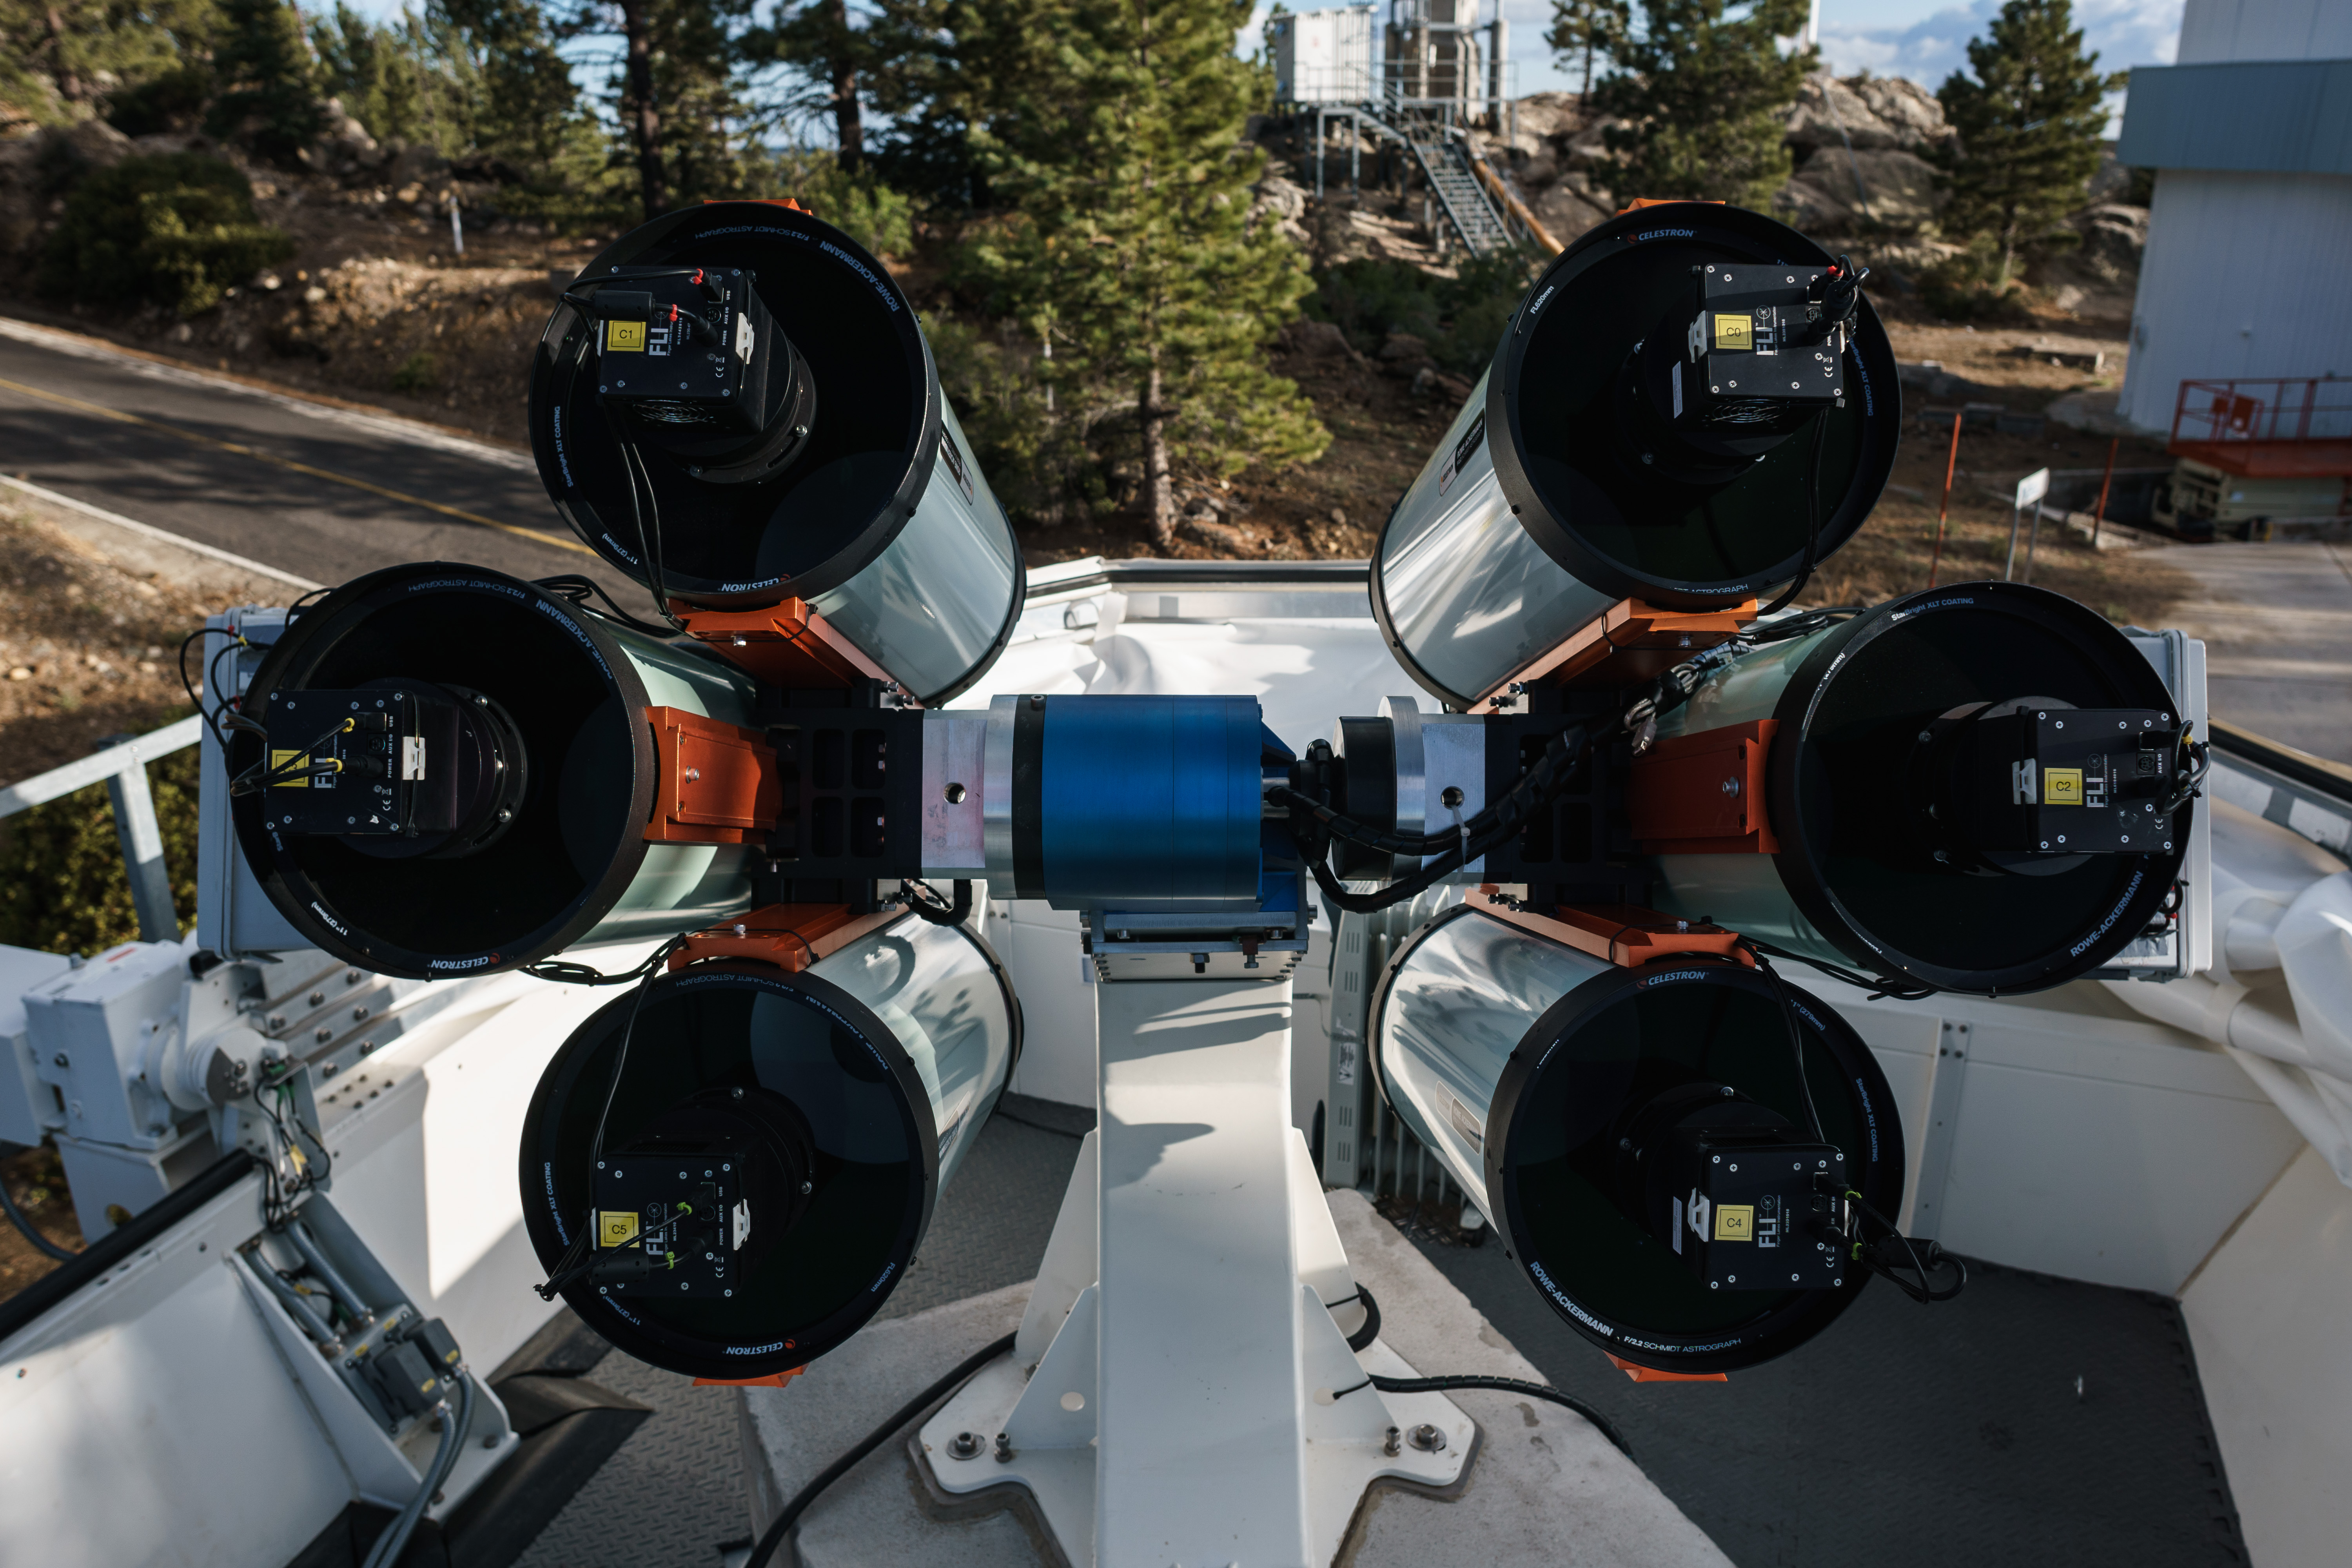
\includegraphics[width=\linewidth]{figures/frontmatter-ddotioan.jpg}

\bigskip
\bigskip
{
\baselineskip=10pt
 \large
 Fernando~Ángeles,
 Rosa~L.~Becerra-Godínez,
 Alejandro~S.~Farah,
 William~H.~Lee,
 Fernando~Quirós,
 Carlos~G.~Román-Zúñiga,
 Carlos~G.~Tejada,
 and
 Alan~M.~Watson
 \par
}
\bigskip
{
 \large
 \itshape 
 Instituto de Astronomía\\
 Universidad Nacional Autónoma de México
 \par
}
\bigskip
{
 \large
 4 December 2020
}
\fi

\end{centering}

\newpage

\pagestyle{plain}

%\twocolumn

\tableofcontents


\chapter{Introduction}
\label{chapter:introduction}

This is the technical manual for the {\projectname}\footnote{http://coatli.astroscu.unam.mx} installation, telescope, and instrument. It has two aims. The first is to provide clear instructions to the OAN/SPM technical staff supporting routine operations. The second is to aid {\projectname} and OAN/SPM technical staff perform preventative and corrective maintenance of the equipment.

For an overview of the {\projectname} project, we recommend our 2016 SPIE paper:

\ifcoatli
\begin{itemize}
\item “\href{bibliography/spie-coatli-2016.pdf}{COATLI: an all-sky robotic optical imager with 0.3 arcsec image quality}”,   Watson et al.\ 2016, Proc.\ SPIE, 9908, 99085O-2
\end{itemize}
\fi

\ifddoti
\begin{itemize}
\item “\href{bibliography/spie-ddoti-2016.pdf}{DDOTI: the deca-degree optical transient imager}”, Watson et al.\ 2016, Proc.\ SPIE, 9910, 99100G
\end{itemize}
\fi

\ifcoatli
{\projectname} has been funded by CONACyT (LN 232649, 260369, and 271117)
and the Universidad Nacional Aut\'onoma de M\'exico (CIC and
DGAPA/PAPIIT IT102715, IG100414, IN109408, and IN109418) and is operated and
maintained by the Observatorio Astron\'omico Nacional and the Instituto
de Astronom{\'\i}a of the Universidad Nacional Aut\'onoma de M\'exico.
\fi

\ifddoti
DDOTI is funded by CONACyT (LN 232649, LN 260369, LN 271117, and 277901), the Universidad Nacional Autónoma de México (CIC and DGAPA/PAPIIT IG100414, IT102715, AG100317, IN109418, IG100820, and IN105921), the NASA Goddard Space Flight Center, and the University of Maryland (NNX17AK54G). DDOTI is operated and maintained by the Observatorio Astronómico Nacional and the Instituto de Astronomía of the Universidad Nacional Autónoma de México. We acknowledge the contribution of Neil Gehrels to the development of DDOTI.
\fi

\part{Operations}

\chapter{Safety}
\label{chapter:safety}


In this manual, safety instructions and observations are highlighted by boxes.
\section{Feedback}

If you encounter a dangerous situation that is specific to {\projectname} and is not covered by the rules below or if you have comments or suggestions on the existing rules, please inform the PIs of {\projectname} (Alan Watson and William Lee) and the Secretario Técnico of the OAN.

\section{Priorities}

\safety{
The safety priorities at the {\projectname} installation, from highest to lowest, are:
\begin{enumerate}
\item Personnel safety: avoiding injury and death to personnel.
\item Equipment safety: avoiding damage or loss of equipment.
\item Observing and data preservation.
\end{enumerate}
}

\section{Personnel Safety}

The {\projectname} installation is potentially one of the most dangerous installations at the OAN/SPM. Personnel safety is more important than equipment safety or observations. The following  rules are designed to maintain personnel safety and must be followed at all times.

\safety{You must not work alone on the open platform or on the balconies.} 

At least one other person must be present either on the platform or at ground level.

\safety{You may work alone on the closed platform. However, someone else must be present when you ascend or descend.}

You should have someone to close the enclosure manually after you have entered and open it manually for you to leave. Remember that you must have a radio on hand.

\safety{You must use a safety harness, line, and helmet whenever you are on the  platform or balconies or to ascend the tower. When you are working on the balcony or another position from which you might fall, attach your line to one of the fasteners, to the balcony rail, or to something equivalently strong. In cold weather, we strongly recommend using gloves.} 

The main platform is about 5 meters above the walkways. A fall from this height can easily kill.

Safety harnesses, lines, and helmets are stored in the shed.

The line can be attached to various points: the eyes in the platform floor installed specifically for this purpose, the balcony safety rails, and other parts of the platform or tower structure.

The helmet will protect you from collisions with the telescopes, if you fall, and from falling objects.

\safety{You must use a safety helmet if you are working under the platform or balconies.}

The main platform is about 5 meters above the walkways. An impact from an object falling from this height can easily kill.

Safety helmets are stored on the shed.

\safety{Transport equipment and tools to and from the platform using the appropriate equipment provided: ropes, locking carabiners, locking hooks, straps, a tool carrier, and an equipment bag.}

Using this equipment in an appropriate manner will significantly reduce the risk of something falling. This equipment is stored in the project cabinet in the ground-floor of the 84-cm telescope. When you use the rope, you can fasten the upper end to one of the eyes in the platform using a locking carabiner. See Figure~\ref{figure:safety-transport}. When lifting heavy equipment to the platform, consider using the locking hook. 

\textcolor{red}{MAGUI: This equipment, shown in Figure~\ref{figure:safety-transport}, is stored in the project cabinet in the ground-floor of the 84-cm telescope. Using this equipment in an appropriate manner will significantly reduce the risk of something falling. When you use the rope, you can fasten the upper end to one of the eyes in the platform using a locking carabiners. When lifting heavy equipment to the platform, consider using the locking hook.}

\begin{figure}
\begin{center}
\resizebox{\linewidth}{!}{
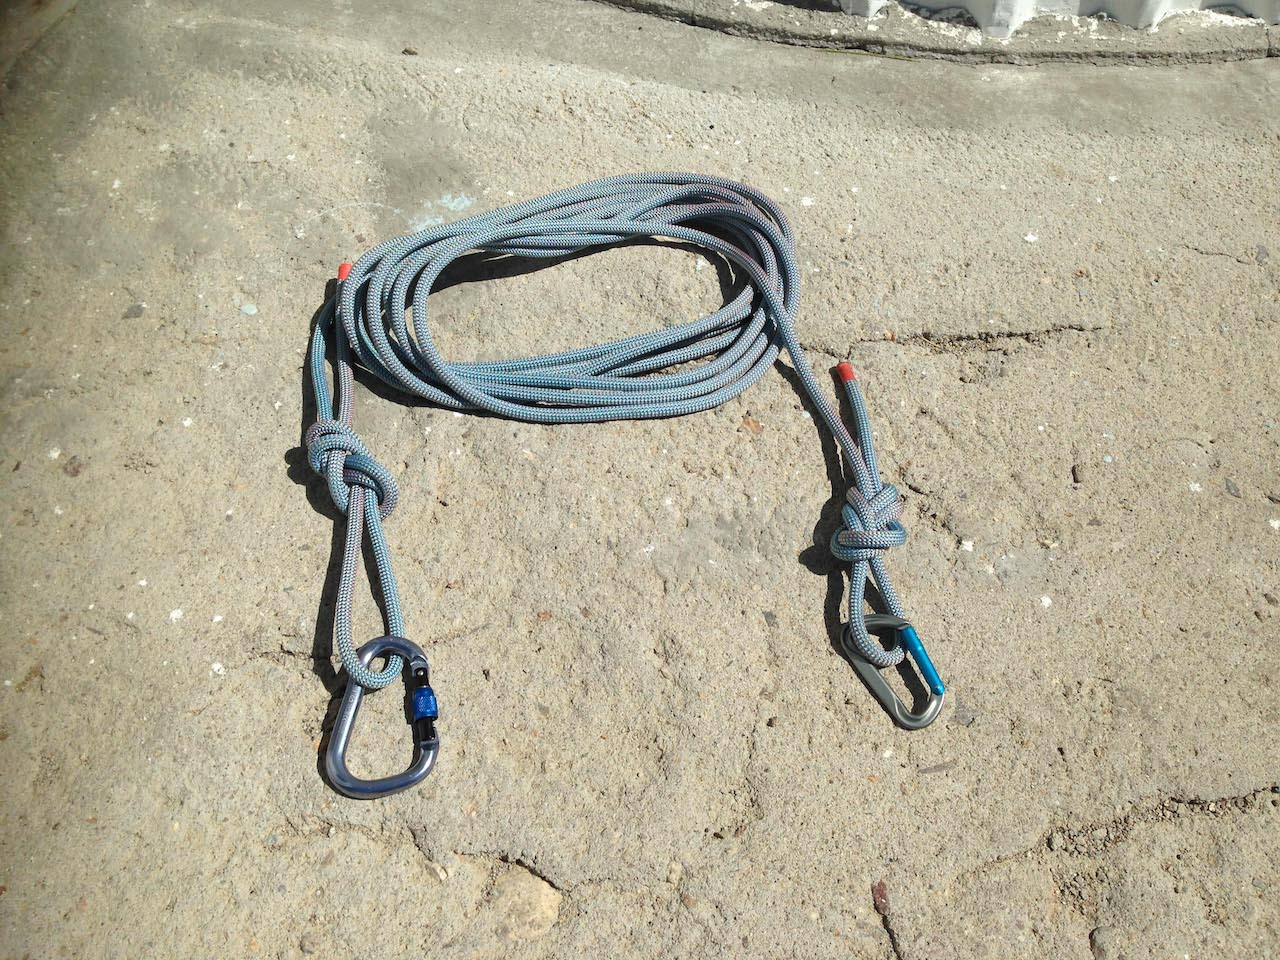
\includegraphics[width=0.50\linewidth]{figures/safety-rope}
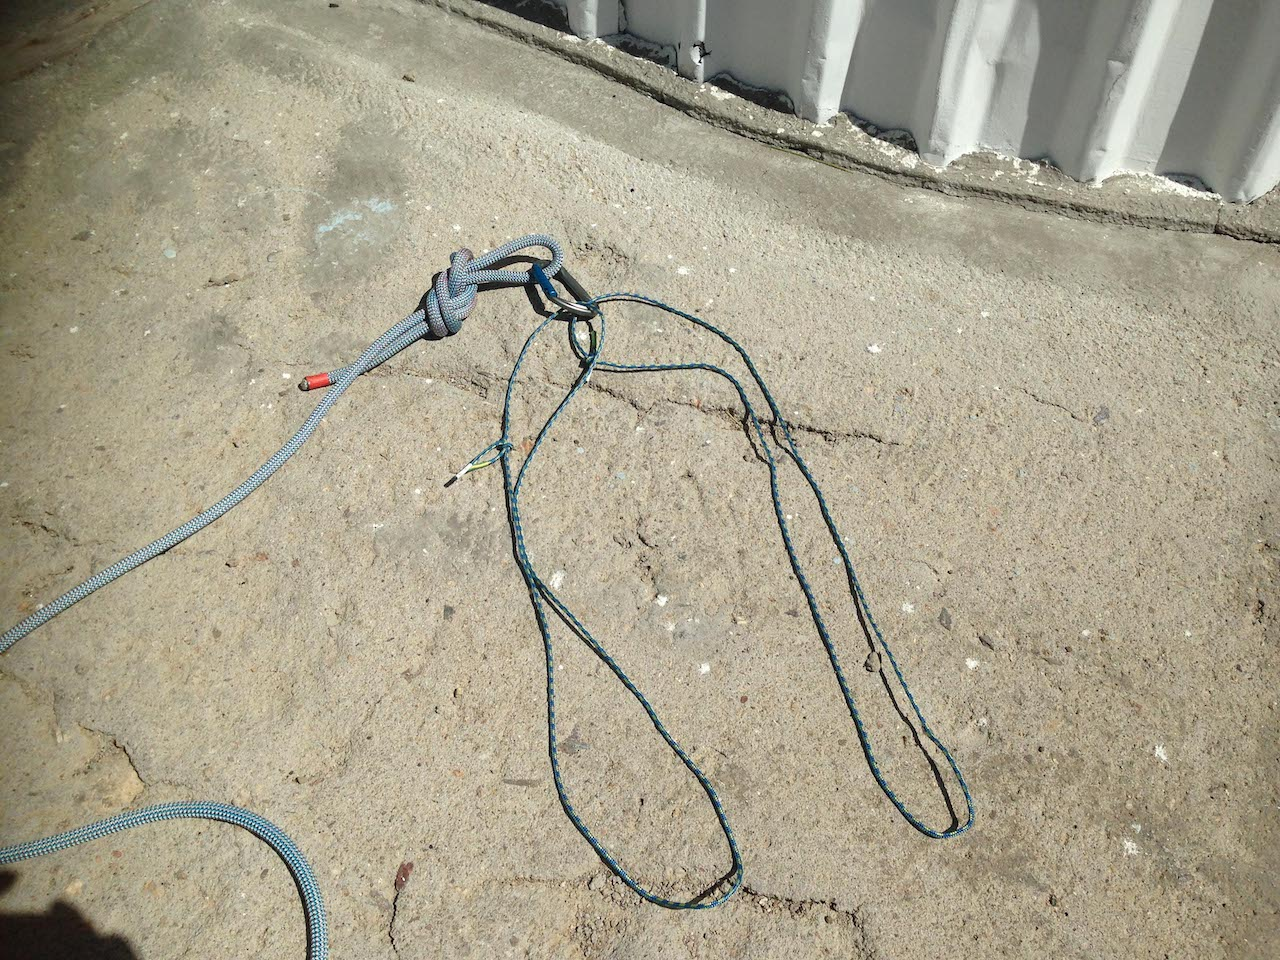
\includegraphics[width=0.50\linewidth]{figures/safety-straps.jpg}
}
\resizebox{\linewidth}{!}{
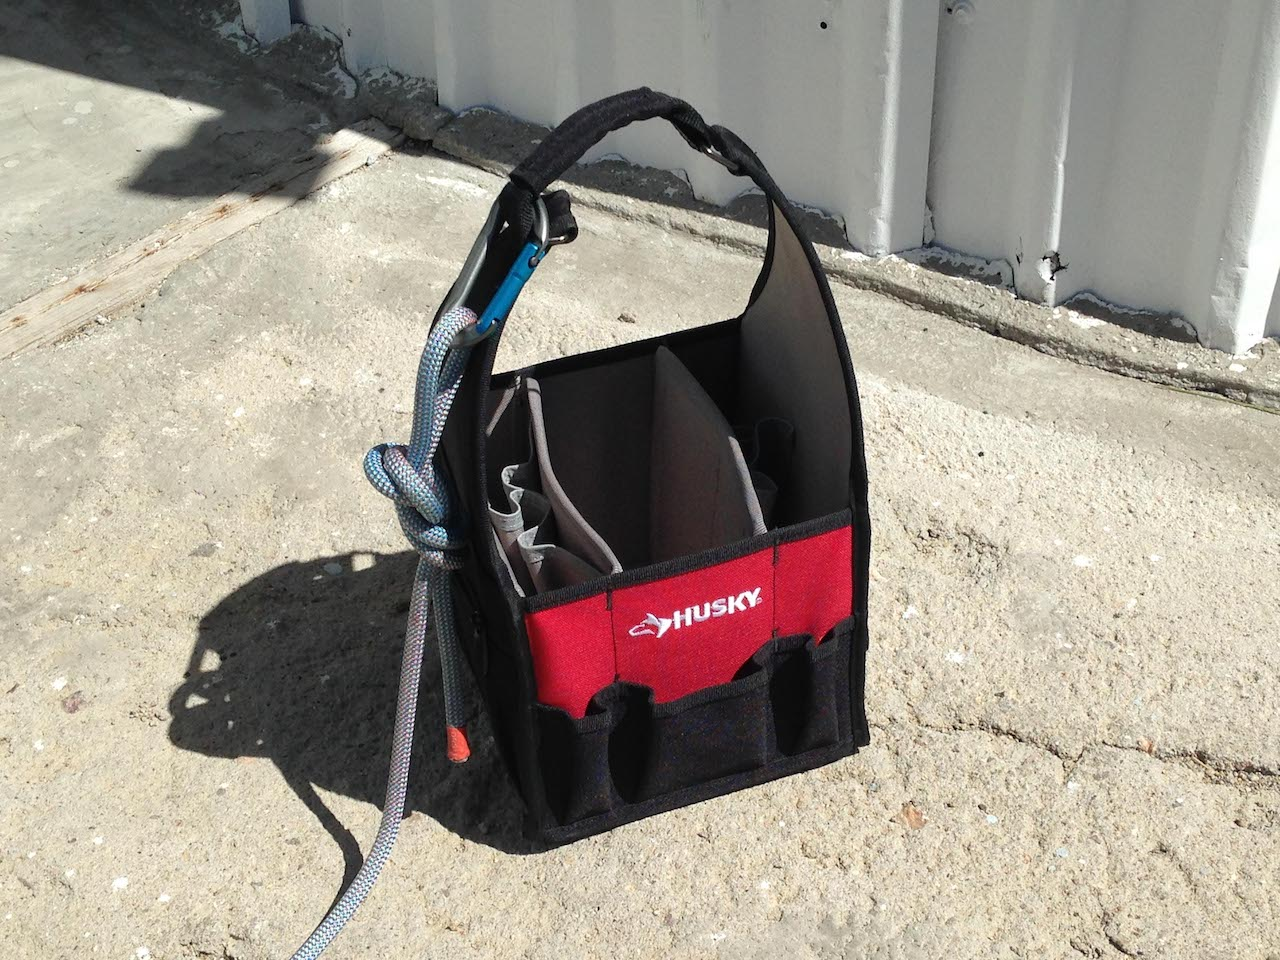
\includegraphics[width=0.50\linewidth]{figures/safety-tools.jpg}
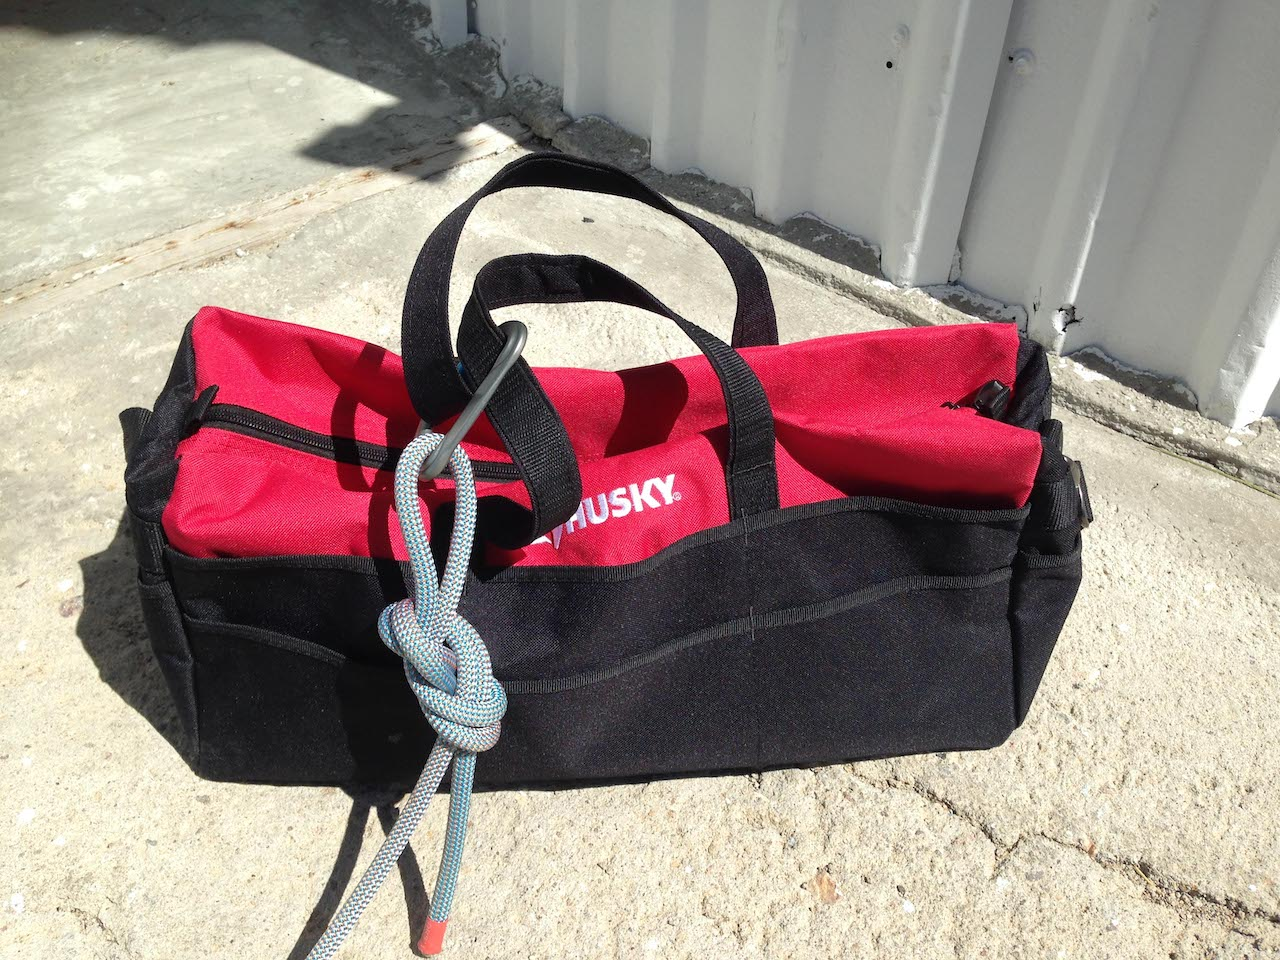
\includegraphics[width=0.50\linewidth]{figures/safety-bag.jpg}
}
\end{center}
\caption{Equipment to safely transport equipment to and from the platform: ropes, locking carabiners, straps, a tool carrier, and an equipment bag.}
\label{figure:safety-transport}
\end{figure}

\safety{Return equipment and tools to their usual storage location when you have finished using them.}

This ensures that equipment can be found when it is next needed. This is especially important for safety equipment.

\safety{If you wish to ascend to the platform or balconies, you must put the enclosure in local mode.}

In remote mode the enclosure can close without warning.

\safety{You may only be on the platform or balconies if it is strictly necessary.}

The platform and balconies are not a vantage points. You must only be on them to work on equipment.

\safety{You may only be on the platform or balconies at night if you need to close the enclosure manually or are testing or commissioning equipment on the sky.}

You must not perform maintenance at night.

If there is a failure at night, you must not ascend to the platform to fix it. Instead, you must abandon the night’s observations and attempt to close the enclosure from the shed. 

You may only ascend to the platform at night if you need to close the enclosure manually.

\safety{You may only be on the platform or balconies in poor conditions if you need to close the enclosure manually.}

Poor conditions include high wind, snow, and rain. 

You must not perform maintenance in poor conditions.

You may only climb the platform in poor conditions if you need to close the enclosure manually.

\safety{Do not walk on the elevated areas at the ends of the platform.}

These areas are not load-bearing. If you walk on them, it is likely that they will collapse and you will fall.

\safety{If you need to summon help and do not have a portable radio, you can use the static emergency radio located between the 84-cm building and DDOTI.} 

\safety{You must physically disconnect mains power before working on an electronics boxes C--F.}

Note that box C has two mains connectors, one for regulated power and one for unregulated power. Boxes D--F have only one mains connector, for regulated power.

Using the switch is not enough; it is present to allow the equipment to be rebooted. Besides, the unregulated power to box C is not switched.

\safety{Be extremely careful when working inside the enclosure, covers, and secondary cabinets as they use 220 VAC.}


\section{Equipment Safety}

\safety{Only open the enclosure explicitly when conditions are benign.
Conditions are not benign if:
\begin{enumerate}
\item It is raining or snowing.
\item The humidity is 85\% or higher and rising or previously reached 90\% and has not yet fallen below 80\%.
\item The wind average speed has been {\windlimit} km/h or greater at any moment in the previous 30 minutes.  
\item There are other circumstance which, in the judgement of observatory technical staff, dictate that it is not safe to open.
\end{enumerate}
}

These rules are implemented in the {\projectname} weather server. If you check the {\projectname} web page, there is a summary line for the weather that says “may be open”, conditions are benign and you may open. If it does not, conditions are not benign and you must not open.

Note that the rules for opening the other telescopes specify a wind limit of 45 km/h. The limit for {\projectname} is currently lower until we have greater confidence in its reliability and performance in high winds.

\safety{Before opening the enclosure, check on the webcams that the telescope is not pointed to towards the sun.}

\ifcoatlioan
In the home position, the telescope is pointed to the northern horizon and on the western side of the mount. This is to protect the telescope mirrors from falling debris or water drops.
\fi
\ifddotioan
In the home position, the telescopes are pointed 30 degrees below the northern horizon. This is to protect the telescope corrector lenses from falling debris or water drops.
\fi


\safety{The enclosure controller should normally be switched on at all times in order to keep the electromagnetic lock activated.}

If the lock is not activated, the wind can open the roof a few centimeters and allow the ingress of rain or snow.

\safety{In case of fire, there is an extinguisher in the shed.}

If you do fight a fire, remember that personnel safety is more important than equipment safety.


\chapter{Interface}
\label{chapter:interface}

This chapter describes the interface used by the observatory staff to interact with the {\projectname} control system.

\section{Access}

The address of the {\projectname} web site is:
\begin{quotation}
\url{\projectinterfaceurl}
\end{quotation}

The web site contains the interface and documentation. The interface is only directly available to computers on the mountain-top network, although ssh port-forwarding can make it indirectly available elsewhere.

The interface is protected by passwords. The \verb|operator15| and \verb|operator21| accounts are configured with the same passwords as the RATIR interface. If in doubt, ask on the Skype chat.



\section{Main Page}

\begin{figure}
\begin{center}
\resizebox{\linewidth}{!}{\begin{labeled}{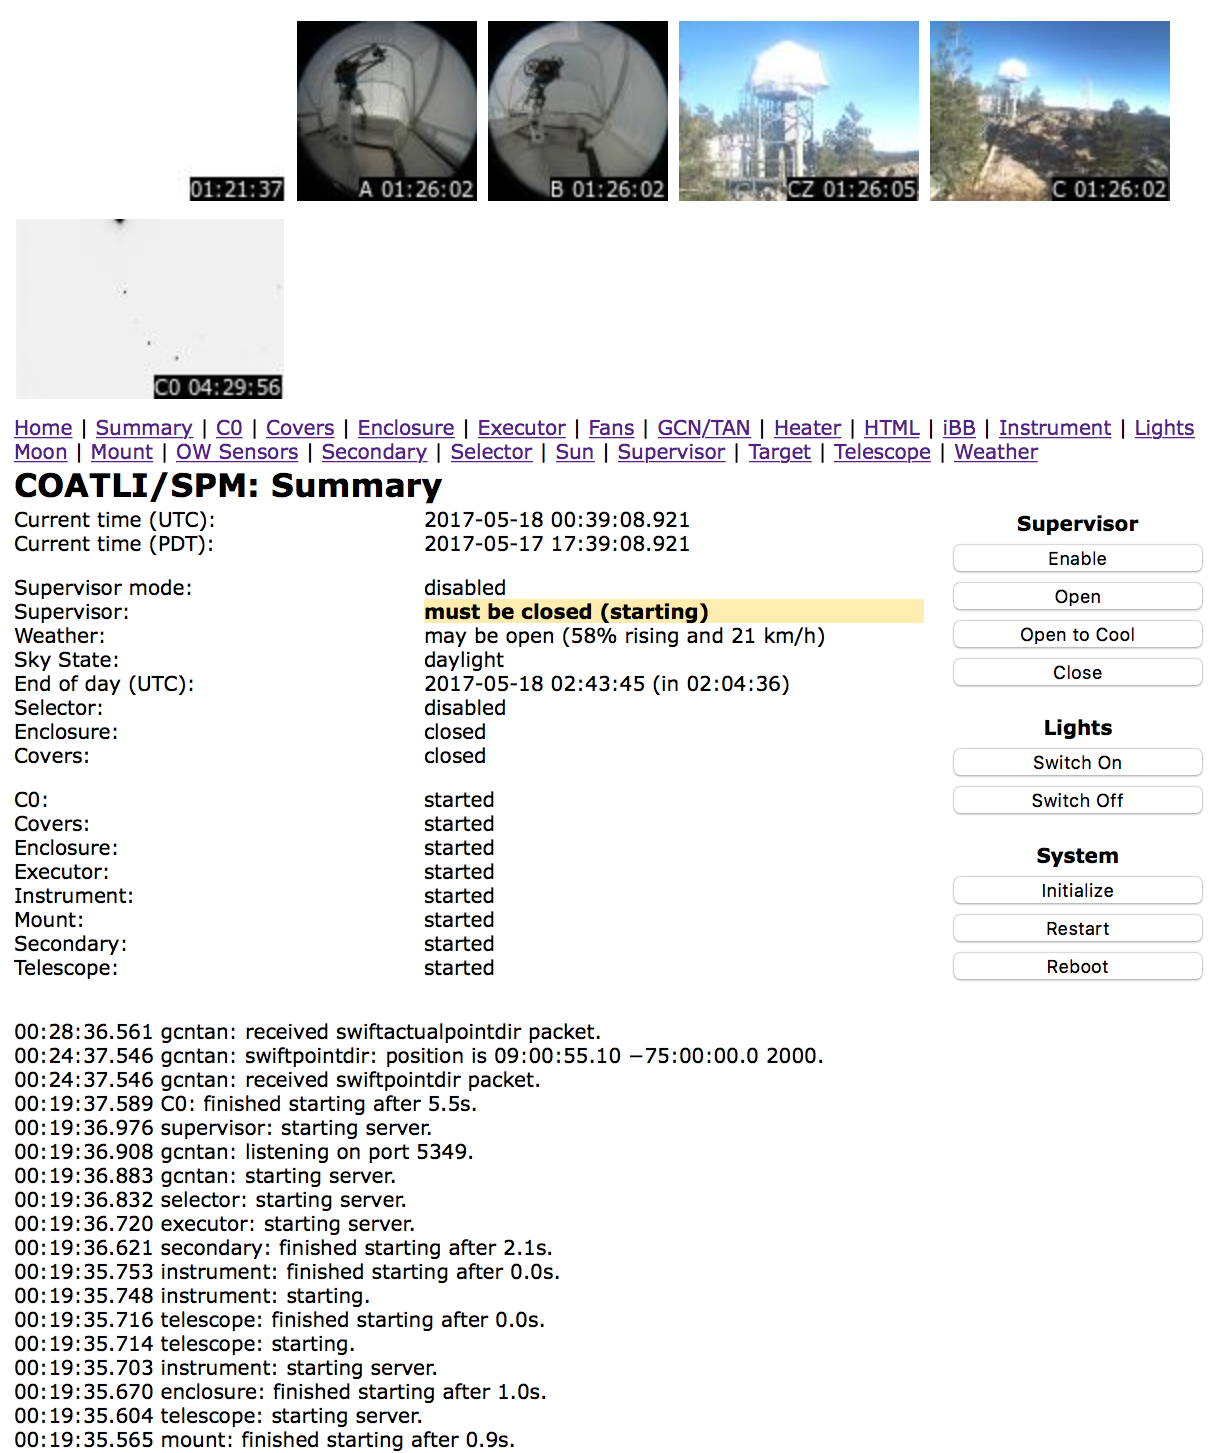
\includegraphics[width=0.8\linewidth]{figures/interface-main-page}}
\arrowandlabel{(-3.6,5.7)}{(-3.6,7)}{south}{All-Sky}
\arrowandlabel{(-1.8,5.7)}{(1,7)}{south}{Webcams}
\arrowonly{(-0.4,5.7)}{(1,7)}
\arrowonly{(+1.0,5.7)}{(1,7)}
\arrowonly{(+3.2,5.7)}{(1,7)}
\arrowandlabel{(-4.8,3.2)}{(-6,3.2)}{east}{C0}
\arrowandlabel{(-4.8,2.2)}{(-6,2.2)}{east}{Navigation}
\arrowandlabel{(-4.8,0.5)}{(-6,0.5)}{east}{Status}
\arrowandlabel{(-4.8,-1.2)}{(-6,-1.2)}{east}{Activity}
\arrowandlabel{(-4.8,-4)}{(-6,-4)}{east}{Log}
\arrowandlabel{(4.8,0.5)}{(6,0.5)}{west}{Buttons}
\end{labeled}}
\end{center}
\caption{An example of the main page of the interface. The major elements are labelled and described in the text.}
\label{figure:interface-main-page}
\end{figure}

\ifcoatlioan

\begin{figure}
\begin{center}
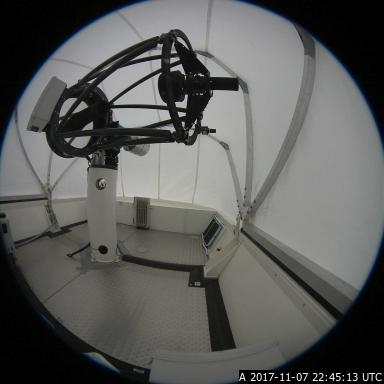
\includegraphics[width=0.8\linewidth]{figures/interface-coatlioan-webcam-a.jpg}
\end{center}
\caption{An example view from webcam A (in N corner of the enclosure looking to the SW).}
\label{figure:interface-webcam-a}
\end{figure}

\begin{figure}
\begin{center}
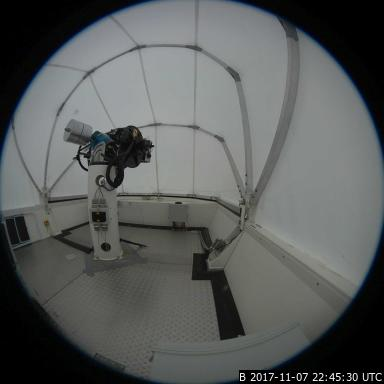
\includegraphics[width=0.8\linewidth]{figures/interface-coatlioan-webcam-b.jpg}
\end{center}
\caption{An example view from webcam B (in S corner of the enclosure looking to the NE).}
\label{figure:interface-webcam-b}
\end{figure}

\begin{figure}
\begin{center}
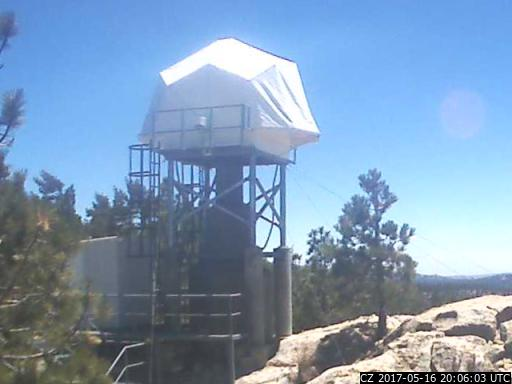
\includegraphics[width=0.8\linewidth]{figures/interface-coatlioan-webcam-cz.jpg}
\end{center}
\caption{An example view from webcam CZ (on the 84-cm telescope building looking towards {\projectname}). Webcam CZ is actually just a fixed zoom of webcam C.}
\label{figure:interface-webcam-cz}
\end{figure}

\begin{figure}
\begin{center}
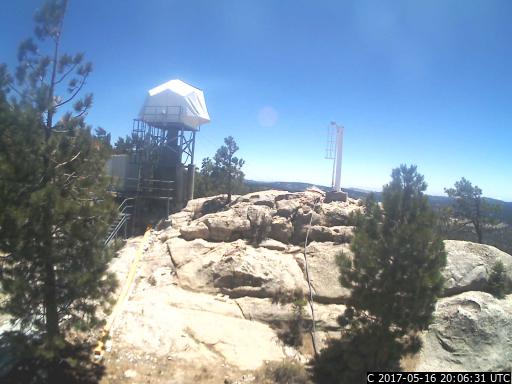
\includegraphics[width=0.8\linewidth]{figures/interface-coatlioan-webcam-c.jpg}
\end{center}
\caption{An example view from webcam C (on the 84-cm telescope building looking towards {\projectname}).}
\label{figure:interface-webcam-c}
\end{figure}

\fi

\ifddotioan

\begin{figure}
\begin{center}
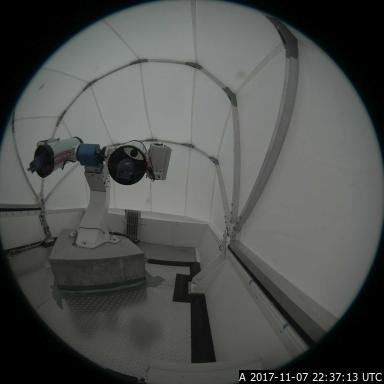
\includegraphics[width=0.8\linewidth]{figures/interface-ddotioan-webcam-a.jpg}
\end{center}
\caption{An example view from webcam A (in N corner of the enclosure looking to the SSW).}
\label{figure:interface-webcam-a}
\end{figure}

\begin{figure}
\begin{center}
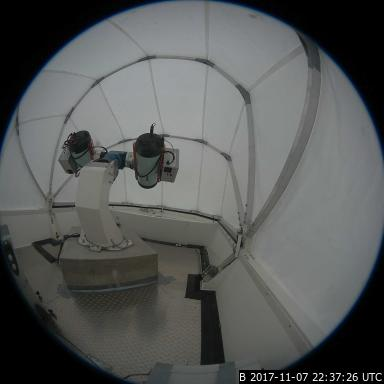
\includegraphics[width=0.8\linewidth]{figures/interface-ddotioan-webcam-b.jpg}
\end{center}
\caption{An example view from webcam B (in S corner of the enclosure looking to the NNE).}
\label{figure:interface-webcam-b}
\end{figure}

\begin{figure}
\begin{center}
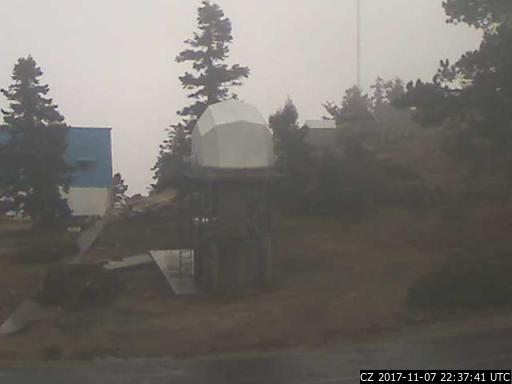
\includegraphics[width=0.8\linewidth]{figures/interface-ddotioan-webcam-cz.jpg}
\end{center}
\caption{An example view from webcam CZ (on the 84-cm telescope building looking towards {\projectname}). Webcam CZ is actually just a fixed zoom of webcam C.}
\label{figure:interface-webcam-cz}
\end{figure}

\begin{figure}
\begin{center}
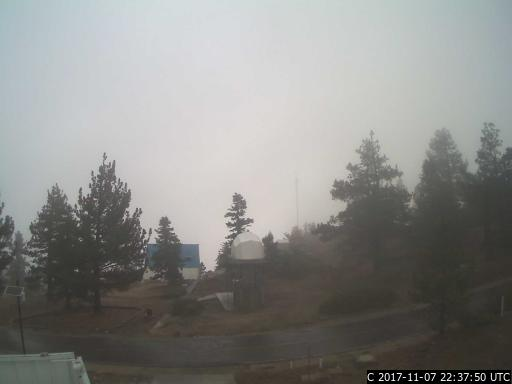
\includegraphics[width=0.8\linewidth]{figures/interface-ddotioan-webcam-c.jpg}
\end{center}
\caption{An example view from webcam C (on the 84-cm telescope building looking towards {\projectname}).}
\label{figure:interface-webcam-c}
\end{figure}

\fi

Figure~\ref{figure:interface-main-page} shows an example of the main page of the interface. The major elements of the interface are:

\begin{itemize}
\item
Thumbnail images from the webcams. Clicking on the thumbnail images brings up larger images, examples of which are shown in Figures~\ref{figure:interface-webcam-a}, \ref{figure:interface-webcam-b}, \ref{figure:interface-webcam-cz}, and \ref{figure:interface-webcam-c}. These images are useful for checking the status of the enclosure and telescope. At night, one needs to switch on the enclosure lights (see \S\ref{interface-switch-on-button}) to see anything in the webcams.  
\item
A thumbnail image from the all-sky camera. Clicking on the thumbnail image brings up a larger image. This is useful for checking for clouds.
\item
A thumbnail image of the latest image taken by the C0 detector. Clicking on the thumbnail image brings up a larger image. This is useful for checking focus.
\item
A navigation section. Clicking on these links will bring up the detailed page for the corresponding control system server. These pages are typically used by the team members to diagnose problems.
\item
A status section. In the main page this gives:
\begin{itemize}
\item
The UTC time.
\item
The civil time at the observatory (PST or PDT).
\item
The supervisor mode (“enabled”, “disabled”, “open”, “opentocool”, or “closed”).
\item
A description of whether the supervisor mode permits the enclosure to be open and why.
\item
A description of whether the current weather conditions permit the enclosure to be open and why (wind, rain, and humidity).
\item
A description of the current sky state (daylight, twilight, and night).
\item
The local end of day time, in UTC (with a count-down clock).

\item
The enclosure state (open or closed).
%\item

\end{itemize}
\item
The activity section. If a control system server activity is not “idle” (for example, if it is “started”, “initializing”, “moving”, “tracking”, “opening”, or “closing”), this is shown here. If a server activity is “idle”, it is not shown here. Thus, if all of the servers are “idle”, this section is empty.

Errors and warnings are shown here in red and yellow respectively.
\item
The log section. This section shows the latest log messages from the control system in reverse order.
\item
The buttons. These are used to interact with the control system.
\begin{itemize}
\item
Enable. Enabled the supervisor. This permits the supervisor to open and close according to the weather and sky state. Note that the supervisor only takes decisions to open, open to cool, or close if it is enabled. 
\item
Open. Force the supervisor to open and to stay open until explicitly instructed otherwise.
\item
Open to Cool. Force the supervisor to open to cool and to stay open to cool until explicitly instructed otherwise. Opening to cool opens the enclosure partially,  and starts to cool the CCD. It is typically used at the end of the day to cool the enclosure, telescope, and CCD ready for observations after sunset.
\item
Close. Force the supervisor  to close and to stay closed until explicitly instructed otherwise.
\label{interface-close-button}
\item
Switch On. Switch on the enclosure lights. This is useful when you want to use the webcams to check the status of the telescope or enclosure. Of course, one does not want to turn the lights on if the telescope is observing.
\label{interface-switch-on-button}
\item
Switch Off. Switch off the enclosure lights. 
\label{interface-switch-off-button}

\item
Restart. Schedule a restart of the control system servers for the top of the next minute. This can be used to recover from software problems.
\label{interface-restart-button}

\end{itemize}
\end{itemize}

\section{Running the Interface on the Access Mac in the Shed}
\label{section:interface-access-mac}

The interface can be run locally on the Access Mac in the Shed.

If you need to log into the Mac, use the “{\projectaccount}” account with password “{\projectaccount}”.

If the interface and Skype are not running, you can select “Open Interface” or “Open Skype” from the script menu in the upper right, as shown in Figure~\ref{figure:interface-scripts-menu}.

\begin{figure}
\begin{center}
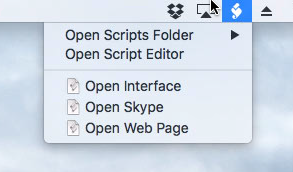
\includegraphics[width=0.4\linewidth]{figures/interface-scripts-menu.png}
\end{center}
\caption{The script menu, in the upper right, can open the interface and Skype on the Access Mac.}
\label{figure:interface-scripts-menu}
\end{figure}

\chapter{Operations}
\label{chapter:operations}

{\projectname} is in regular robotic operation under the responsibility of the observatory staff. Weather permitting, {\projectname} will operate from 30 minutes before sunset to the end of morning astronomical twilight.

\section{Participants}

By “observatory staff” we refer to the telescope operators, resident astronomers, and maintenance technicians. The actually division of responsibilities will be decided by the Secretario Técnico of the observatory.

By “team members” we refer to members of the {\projectname} technical teams.

\section{Communications}

Communication between the observatory staff and the team will take place primarily through the RATIR/COATLI/DDOTI operations Skype chat.

\section{Daily Operations}

The daily operating procedure is:

\begin{enumerate}

\item At the latest one hour before sunset, the observatory staff will carry out a review of the {\projectname} installation. 

This revision has three elements. The observatory staff will:

\begin{enumerate}
\item
Check that all of the control system servers are not showing errors in the web interface. 
\item
Check that the webcams in the web interface are not showing an unusual situation.
\item
If necessary, carry out an on-site inspection of {\projectname}. For example, after a snowfall, it might not be obvious from the webcams whether snow remains on the roof of the enclosure.
\end{enumerate}

If the observatory staff consider that decisions to open and close the installation can be safely taken by the control system, they will enable the supervisor by pressing the “Enable” button in the “Supervisor” section of the web interface.

If the observatory staff consides that decisions to open and close the installation cannot be safely taken by the control system, they should explicitly force the supervisor to maintain the telescope closed by pressing the “Close” button in the “Supervisor” section of the web interface. 

The observatory staff will report the result of their inspection in the Skype chat and will indicate whether they are enabling the supervisor or forcing it to close.

\item
If the supervisor is enabled and weather conditions are benign, the control system will:
\begin{enumerate}
\item
Open partially to cool about half an hour before sunset;
\item
Open completely to observe at sunset; and
\item
Close at the end of morning astronomical twilight.
\end{enumerate}

If the supervisor is enabled and weather conditions are not benign, the control system will not open (if closed) or will close (if open).

If the supervisor is enabled and weather conditions change from not benign to benign, the control system will open partially to cool (between half and hour before sunset and sunset) or open completely to observe (between sunset and the end of morning astronomical twilight).

\item
The supervisor considers weather conditions to be \emph{not benign} if:
\begin{enumerate}
\item It is raining or snowing.
\item The humidity is 85\% or higher and rising or previously reached 90\% and has not yet fallen below 80\%.
\item The wind average speed has been 30 km/h or greater at any moment in the previous 30 minutes.  
\end{enumerate}
Note that the rules for opening the other telescopes specify a wind limit of 45 km/h. The limit for {\projectname} is currently lower until we have greater confidence in its reliability and performance in high winds.

\item
The observatory staff will monitor {\projectname} during the night. Their primary responsibilities are:
\begin{enumerate}
\item If the observatory staff consider that decisions to open and close the installation can be safely taken by the control system, they should enable the supervisor by pressing the “Enable” button in the “Supervisor” section of the web interface and report this in the Skype chat.
\item If the observatory staff consider that decisions to open and close the installation cannot be safely taken by the control system, they must explicitly force the supervisor to maintain the telescope closed by pressing the “Close” button in the “Supervisor” section of the web interface and report this in the Skype chat. 
\item
The observatory staff should verify that the the control system opens and closes as expected according to the weather conditions and the state of the supervisor. If it does not close, they should intervene as described in \S\ref{section:operations:interventions}.

\item
When the control system closes (at the end of the night, in response to weather conditions, or if the supervisor is forced to close), it switches the lights on for safety. At the end of the process, if the control system can determine that the enclosure closed correctly, it will switch the lights off. If it cannot, it will leave the lights switched on. Thus, if the lights are left on, this indicates that there was a problem during closing and the observatory staff should intervene as described in \S\ref{section:operations:interventions}.

\item
The observatory staff should report explicit changes to the supervisor state (e.g., use of the “Enable” and “Close” buttons) and any other relevant information in the Skype chat.
\end{enumerate}

As their other duties permit, the observatory staff are encouraged to report other conditions or occurrences that might degrade the ability of the telescope to observe (e.g., failures of the control system or failures to focus) in the Skype chat.

\item
During the evening and night, interventions by the observatory staff are limited to whatever is necessary to close {\projectname} and return it to a safe state. Once the observatory staff have intervened, {\projectname} must be closed and may not open again until the next day.

\item
Requests by team members for interventions beyond those needed to close {\projectname} correctly will be directed to the Secretario Técnico of the observatory.
\end{enumerate}

\section{Interventions to Close}
\label{section:operations:interventions}

The control system should normally operate without problems and with minimal action on the part of the observatory staff beyond setting the supervisor mode. However, in the event of a failure, the observatory staff may need to intervene to close.

If the control system does not close when expected or does not close correctly, the observatory staff should:

\begin{enumerate}
\item
First attempt to close normally:
\begin{enumerate}
\item
Press the “Close” button in the supervisor section of the interface (see \S\ref{interface-close-button}). This should turn on the enclosure lights and close.
\item
Check the interface and webcams for success or failure.
\end{enumerate}
\item
If that fails, attempt an emergency close:
\begin{enumerate}
\item
Press the “Emergency Close” button in the supervisor section of the interface (see \S\ref{interface-close-button}). This should turn on the enclosure lights and close.
\item
Check the interface and webcams for success or failure.
\end{enumerate}
\item
If that fails, close the enclosure locally according to the procedure in \S\ref{section:enclosure-opening-or-closing-in-local-mode}.
\item
If that fails, close the enclosure manually according to the procedures in %\S\ref{section:enclosure-manual-opening-or-closing-with-power} or
\S\ref{section:enclosure-manual-opening-or-closing-without-power}.
\end{enumerate}

\section{Weekly Inspection}

The observatory staff should carry out a physical inspection of the installations during daytime at least once per week (if weather conditions permit). The Secretario Técnico will determine the schedule for this inspection.

\subsubsection{Safety Considerations}

\safety{You must use a safety harness, line, and helmet whenever you are on the  platform or balconies or ascend the tower. Attach your line to one of the fasteners, to the balcony rail, or to something equivalently strong.} 

\safety{You must use a safety helmet if you are working under the platform or balconies.}

\subsubsection{Requirements}

You will need:
\begin{itemize}
\item At least two persons.
\item The key to the shed (see \S\ref{section:shed}).
\item Weather conditions adequate for opening the enclosure and ascending to the platform.
\end{itemize}

\subsubsection{Procedure}

\begin{enumerate}
\item
Verify that there is a fire extinguisher in the shed.
\item 
Verify that the web interface and the Skype chat are open on the control Mac in the shed. If they are not, open them by following the procedures in \S\ref{section:interface-access-mac}.
\item 
Inspect the inside of the shed. 
\item 
Inspect the columns and underside of the platform.
\item
Open the enclosure locally using the procedure in \S\ref{section:enclosure-opening-or-closing-in-local-mode}.
\item
One person should ascend to the platform to inspect: the electronics boxes, the instrument, the telescope, the mount, and the platform.
\item
Close the enclosure locally using the procedure in \S\ref{section:enclosure-opening-or-closing-in-local-mode}, but leave the enclosure controller in local mode.
\item
The person on the platform should inspect the enclosure roof from the inside.
\item
Open the enclosure locally using the procedure in \S\ref{section:enclosure-opening-or-closing-in-local-mode}.
\item
The person on the platform should descend.
\item
Leave the enclosure controller in remote mode.
\item
Report that the revision has been carried out in the Skype chat. Additionally, report any anomalies in the Skype chat.
\end{enumerate}

\section{Soft Shut-Down and Start-Up}

A “soft” shut-down is appropriate for circumstances in which electrical power will continue to be supplied to {\projectname}. This is the normal situation over the winter break. In this case, we can leave the computers on and rely on the electromagnet to maintain the enclosure closed.

\subsection{Soft Shut-Down}
\label{section:soft-shut-down}

\subsubsection{Safety Considerations}

\safety{You must use a safety harness, line, and helmet whenever you are on the  platform or balconies or ascend the tower. Attach your line to one of the fasteners, to the balcony rail, or to something equivalently strong.} 

\safety{You must use a safety helmet if you are working under the platform or balconies.}

\safety{The enclosure controller cabinet uses 220 VAC. Switch off the power using the switch on the door before working inside the cabinet.}

\subsubsection{Requirements}

You will need:
\begin{itemize}
\item At least two persons.
\item The key to the shed (see \S\ref{section:shed}).
\item Weather conditions adequate for opening the enclosure and ascending to the platform.
\ifddotioan
\item A clean tarpaulin, one long rope,  and one short red cord
\fi
\ifcoatlioan
\item A clean tarpaulin and one short red cord.
\fi
You can find clean tarpaulins in the shelves next to the cabinet in the 84-cm and rope in the tool-drawer of the cabinet.
\end{itemize}

\subsubsection{Procedure}

\begin{enumerate}

\item
Place the enclosure in local mode.

Move the enclosure controller mode selector switch to “LOCAL”.
\item
If the weather permits, open the enclosure to 60 deg.

Set the angle selector switch to 60 deg and then press and hold the open button until the green light goes out.

\item
Both persons should ascend to the platform.

\item
\ifcoatlioan
Verify that the telescope is in the parked position, pointed at the northern horizon with the telescope on the west side of the pillar. If not, release the break on the mount by pressing the “BREAK” button and move it to this position.
\fi
\ifddotioan
Move the telescope so that it is pointed vertically with the CCDs on the bottom and the focusers on the top. To move the telescope, release the brake on the mount by pressing the “BRAKE” button.
\fi

\item
Press the mount emergency stop button.

\begin{figure*}
\ifcoatlioan
\begin{center}
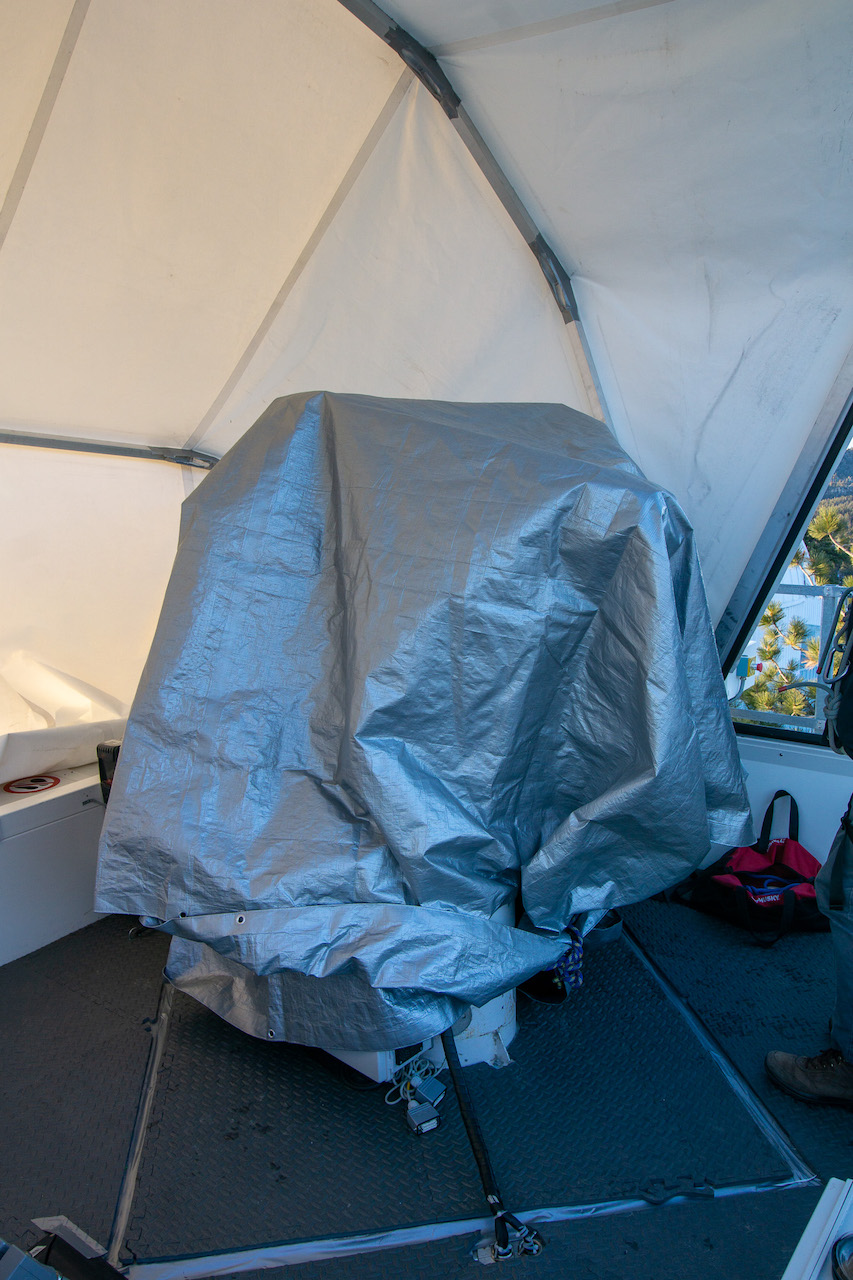
\includegraphics[width=0.65\linewidth]{figures/tarpaulin-coatlioan.jpg}
\end{center}
\caption{The telescope covered by a tarpaulin.}
\fi
\ifddotioan
\begin{center}
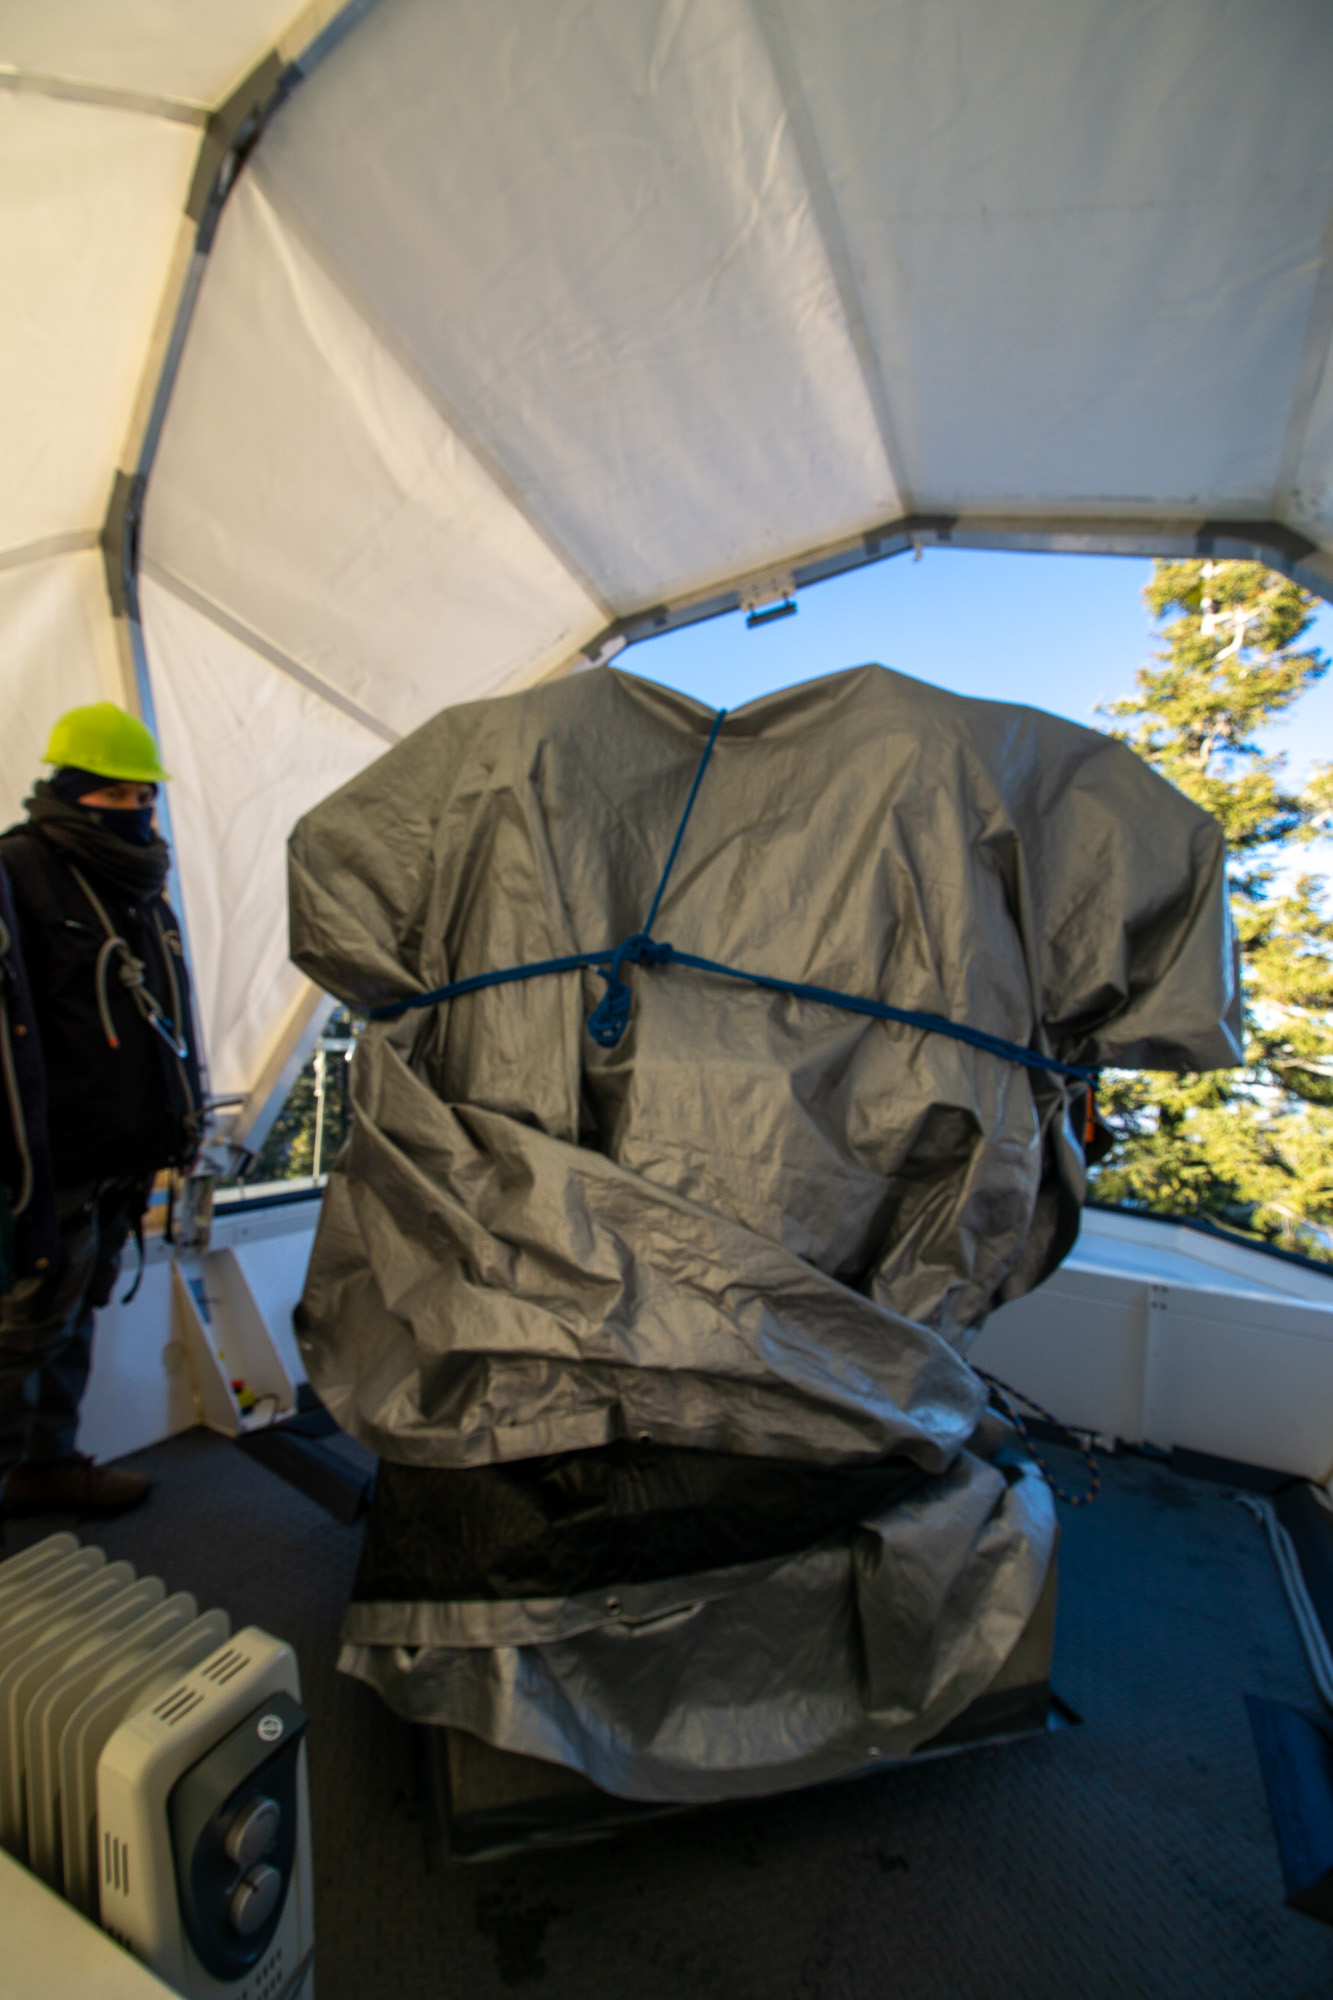
\includegraphics[width=0.45\linewidth]{figures/tarpaulin-ddotioan.jpg}
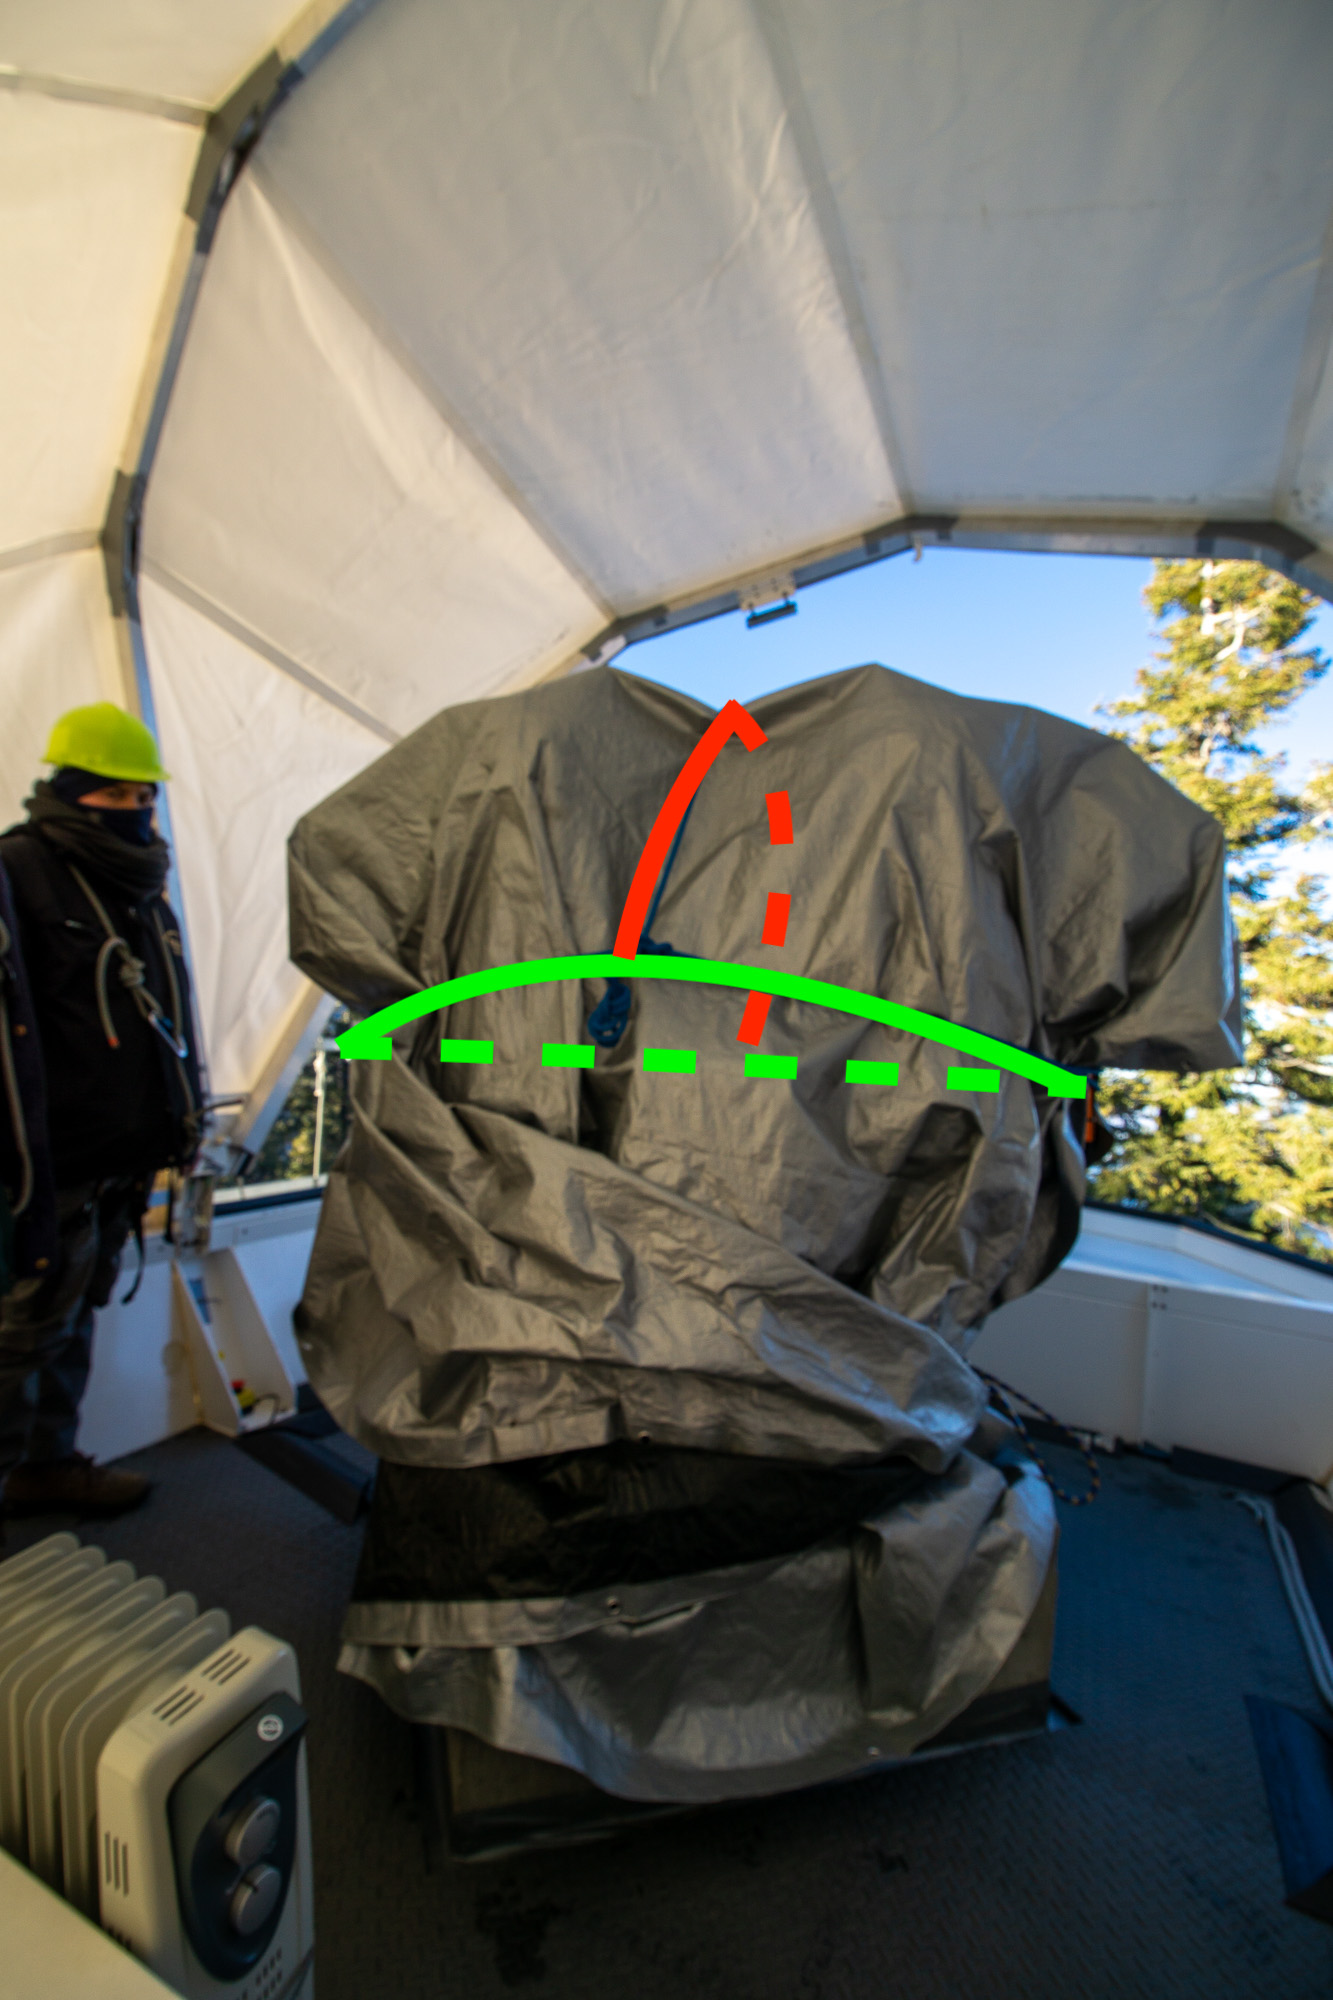
\includegraphics[width=0.45\linewidth]{figures/tarpaulin-ddotioan-annotated.jpg}
\end{center}
\caption{The telescope covered by a tarpaulin. The rope should go around the telescopes (green lines on the right, solid in front and dashed behind), below the two electronics boxes but above the lower end of the telescopes and the CCDs, and then over the the telescopes (red lines on the right), between the east and west sets, and fasten on itself to prevent it slipping down. The loose ends of the tarpaulin should be gathered and tied with a short red rope.  The tarpaulin and the ropes must not come into contact with the CCDs and must not place any stress on them.}
\fi
\label{figure:tarpaulin}
\end{figure*}

\item
Cover the telescope with a tarpaulin.
\ifcoatlioan
Gather the loose ends of the tarpaulin below and fasten them with a short red cord. See Figure~\ref{figure:tarpaulin}.
\fi
\ifddotioan
Be very careful not to place stress on the CCDs.

Wrap the long rope around the telescopes and tarpaulin, below the two electronics boxes but above the lower end of the telescopes and the CCDs, and then pass a loop over the the telescopes, between the east and west sets, and fasten the rope on itself to prevent it slipping down. Gather the loose ends of the tarpaulin below and fasten them with a short red cord. See Figure~\ref{figure:tarpaulin}.

\emph{We repeat. The tarpaulin and the ropes must not come into contact with the CCDs and must not place any stress on them. The tarpaulin and ropes can only come into contact with the telescope tubes, focusers, and electronics boxes.}

\fi

\item
Descend from the platform.

\item 
Close the enclosure.

Press and hold the close button until the green light goes out.

\item
Switch off the enclosure controller.

Move the main power switch on the controller door from ON to OFF.
\item
Open the enclosure controller.

\item
Engage the manual lock. This switches on the enclosure electromagnet and actuates the enclosure emergency stop buttons. This ensures that the electromagnet stays energized even if the PLC fails and that the PLC cannot attempt to open the enclosure.

Move the manual lock switch inside the enclosure controller from OFF to ON. See Figure~\ref{figure:enclosure-controller-manual-lock-switch}.

\item
Close the enclosure controller.

\item
Switch on the enclosure controller.

Move the main power switch on the controller door from OFF to ON.

\item
Place the enclosure in remote mode.

Move the enclosure controller mode selector switch to “REMOTE”.

\item
\ifcoatlioan
Make sure the “PROHIBIDO EL PASO” sign is left in position at the bottom of the access stairs.
\fi
\ifddotioan
Make sure the “PROHIBIDO EL PASO” signs are left in position at the bottom of the access ladders.
\fi

\item
Leave the shed locked. Return the shed keys to the tool box (see \S\ref{section:shed}).

\end{enumerate}

\subsection{Soft Start-Up}
\label{section:soft-start-up}

\subsubsection{Safety Considerations}

\safety{You must use a safety harness, line, and helmet whenever you are on the  platform or balconies or ascend the tower. Attach your line to one of the fasteners, to the balcony rail, or to something equivalently strong.} 

\safety{You must use a safety helmet if you are working under the platform or balconies.}

\safety{The enclosure controller cabinet uses 220 VAC. Switch off the power using the switch on the door before working inside the cabinet.}

\subsubsection{Requirements}

You will need:
\begin{itemize}
\item At least two persons.
\item The key to the shed (see \S\ref{section:shed}).
\item Weather conditions adequate for opening the enclosure and ascending to the platform.
\end{itemize}

\subsubsection{Procedure}

\begin{enumerate}

\item
In the shed, switch off the enclosure controller.

Move the main power switch on the controller door from ON to OFF.

\item
Open the enclosure controller.

\item
Disengage the manual lock.

Move the manual lock switch inside the enclosure controller from ON to OFF. See Figure~\ref{figure:enclosure-controller-manual-lock-switch}.

\item
Close the enclosure controller.

\item
Switch on the enclosure controller.

Move the main power switch on the controller door from OFF to ON.

\item
Place the enclosure in local mode.

Move the enclosure controller mode selector switch to “LOCAL”.

\item
If the weather permits, open the enclosure to 60 deg.

Set the angle selector switch to 60 deg and then press and hold the open button until the green light goes out.

\item
Both persons should ascend to the platform.

\item
Remove the tarpaulin from the telescope.

\item Disengage the mount emergency stop button.

\item
\ifcoatlioan
Verify that the telescope is in the parked position, pointed at the northern horizon with the telescope on the west side of the pillar. If not, release the break on the mount by pressing the “BREAK” button and move it to this position.
\fi
\ifddotioan
Move the telescope to the parked position, pointed just below the northern horizon. To move the telescope, release the brake on the mount by pressing the “BRAKE” button.
\fi

\item Descent from the platform.

\item Close the enclosure. 

Press and hold the close button until the green light goes out.

\item
Place the enclosure in remote mode.

Move the enclosure controller mode selector switch to “REMOTE”.

\item
\ifcoatlioan
Make sure the “PROHIBIDO EL PASO” sign is left in position at the bottom of the access stairs.
\fi
\ifddotioan
Make sure the “PROHIBIDO EL PASO” signs are left in position at the bottom of the access ladders.
\fi

\item
Leave the shed locked. Return the shed keys to the tool box (see \S\ref{section:shed}).

\item
Store the tarpaulin in the shelves next to the cabinet in the 84-cm and the rope in the tool-drawer of the cabinet.

\end{enumerate}

\section{Hard Shut-Down and Start-Up}

A “hard” shut-down is appropriate for circumstances in which electrical power will not continue to be supplied to {\projectname}. This occured, for example, in the evacuations for COVID-19. In this case, we can must shut down the computers and cannot rely on the electromagnet to maintain the enclosure closed.

\subsection{Hard Shut-Down}

\subsubsection{Requirements}

You will need:

\begin{itemize}
    \item Two people plus the participation of a remote team member.
    \item The key to the shed (see \S\ref{section:shed-key}).
    \item Weather conditions adequate for opening the enclosure and ascending to the platform.
    \item The tarpaulin and ropes required for the soft shut-down (see \S\ref{section:soft-shut-down}).
    \item The two riveted plates, a riveter, and rivets.
\end{itemize}

\subsubsection{Procedure}

\begin{enumerate}
\item Perform a soft shut-down (see \S\ref{section:soft-shut-down}).
\item Communicate with the remote team member. They will:
\begin{enumerate}

   \item Log into a computer on the CU, Ensenada, or OAN networks of the Instituto de Astronomía (in order to gain ssh access to the firewall):
   
\begin{quote}\footnotesize
\begin{verbatim}
$ ssh user@somewhere.astrosxx.unam.mx -p 2222 -A -L 8080:localhost:8080
\end{verbatim}
\end{quote}

    \item Log into the firewall:
\begin{quote}\footnotesize
\begin{verbatim}
somewhere$ ssh user@ddoti.astrossp.unam.mx -p 2222 -A -L 8080:localhost:80
\end{verbatim}
\end{quote}

    \item Halt the computer \verb|access|:

\begin{quote}\footnotesize
\begin{verbatim}
firewall$ ssh user@10.0.1.2
access$ sudo shutdown -h -u now
\end{verbatim}
\end{quote}
    
    \item Switch off \verb|access| from \verb|ibb-127|.
\begin{quote}\footnotesize
\begin{verbatim}
firewall$ telnet 10.0.1.5
> get device #1
> set device #1 outlet <n> off
...
\end{verbatim}
\end{quote}
To log out of the iBootBar, use CTRL-] and then \verb|quit|.

    \item Halt the computers \verb|services|, \verb|control|, \verb|c0|, \verb|d0|, \verb|d1|, \verb|d2|, \verb|d3|, \verb|e0|, \verb|e1|, \verb|e2|, \verb|e3|:

\begin{quote}\footnotesize
\begin{verbatim}
firewall$ ssh ddoti@10.0.1.3
services$ sudo haltsoon
\end{verbatim}
\end{quote}

    \item Switch off \verb|instrument|, \verb|platform|, \verb|services|, \verb|control|, and \verb|mount| from \verb|ibb-127|.

\begin{quote}\footnotesize
\begin{verbatim}
$ ssh user@ddoti.astrossp.unam.mx -p 2222
firewall$ telnet 10.0.1.5
> get device #1
> set device #1 outlet <n> off
...
\end{verbatim}
\end{quote}
To log out of the iBootBar, use CTRL-] and then \verb|quit|.
    \item Halt the computer \verb|firewall|.

\begin{quote}\footnotesize
\begin{verbatim}
$ ssh user@ddoti.astrossp.unam.mx -p 2222 -L8080:localhost:80
\end{verbatim}

Open a browser to \verb|http://localhost:8080/| and halt the firewall from the web interface (selevct “Halt System” on the “Diagnostics” menu).
\end{quote}

\end{enumerate}

\item Switch off the two UPSes, the 127 V UPS and the 220 V UPS.

On both UPSes, press the power button on the front panel for three seconds. The UPS will start to beep and will then switch off.

\item Switch off the power supply to the two UPSes.

Open the breaker panel on the wall next to the door. Switch off circuits A and B.

\item
Install the two riveted two plates, one on each side of the enclosure, that hold it closed. See Figure~\ref{figure:riveted-plates}.

\begin{figure*}
\begin{center}
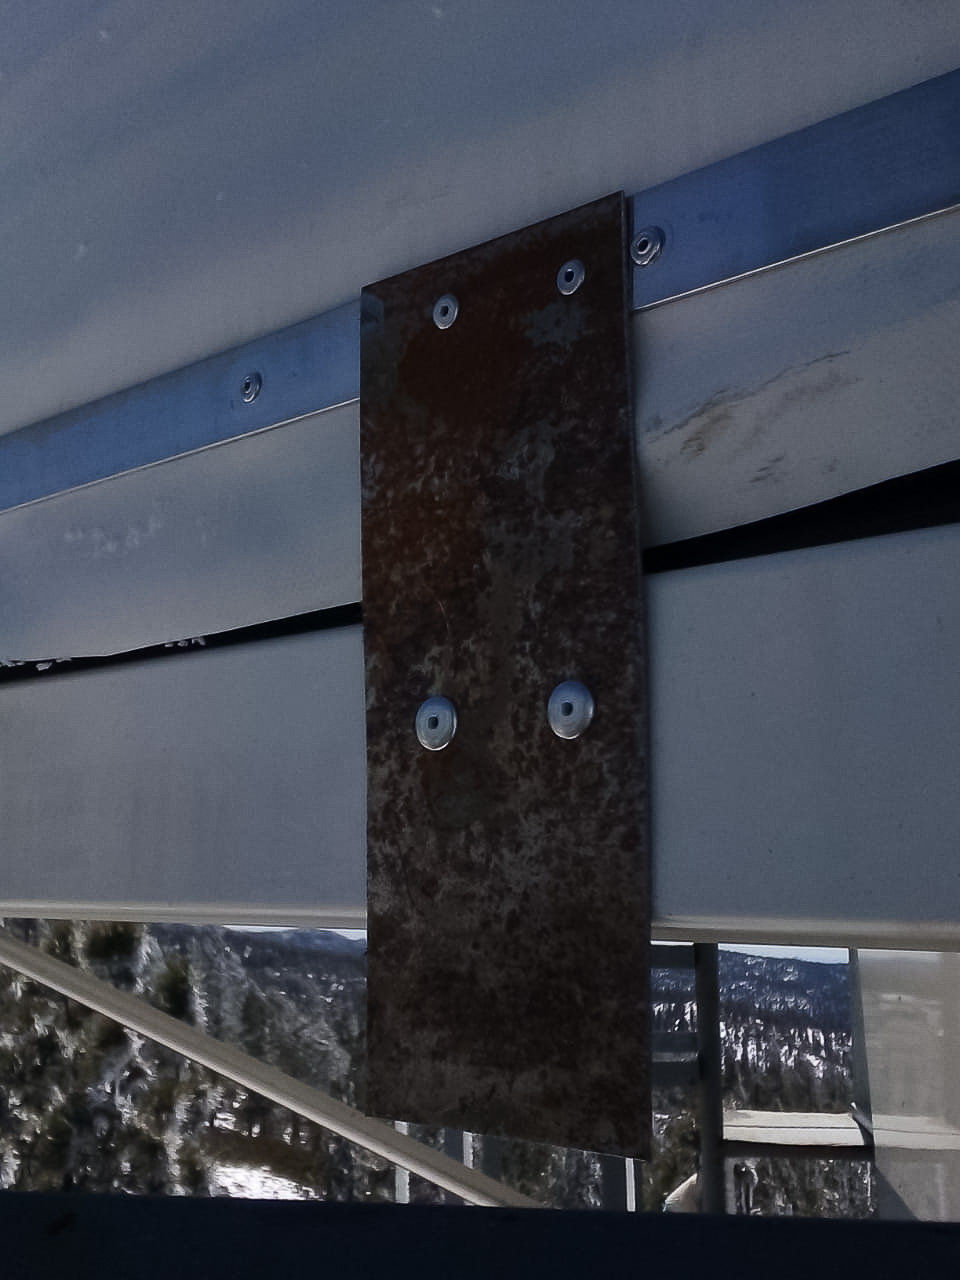
\includegraphics[width=0.45\linewidth]{figures/operations-riveted-plate.jpg}
\end{center}
\caption{One of the riveted plates that hold the enclosure closed when power is switched off.}
\label{figure:riveted-plates}
\end{figure*}

\end{enumerate}

\subsection{Hard Start-Up}

\subsubsection{Requirements}

You will need:
\begin{itemize}
\item At least two persons.
\item The key to the shed (see \S\ref{section:shed}).
\item Weather conditions adequate for opening the enclosure and ascending to the platform.
\item A drill (to remove the riveted plates).
\end{itemize}

\subsubsection{Procedure}

\begin{enumerate}
\item
Remove the two riveted two plates, one on each side of the enclosure, that hold it closed. See Figure~\ref{figure:riveted-plates}.

\item Switch on the power supply to the two UPSes.

Open the breaker panel on the wall next to the door. Switch on circuits A and B.

\item Switch on the two UPSes, the 127 V UPS and the 220 V UPS.

On both UPSes, press the power button on the front panel for at least one second.

\item Switch on the computer \verb|access|.

Press the button on the rear right of the computer.

\item Communicate with the remote team member. They will:

\begin{enumerate}
    \item Switch on the computers \verb|instrument|, \verb|platform|, \verb|services|, \verb|control|, and \verb|access| from \verb|ibb-127|.
    \item Verify that all of the computers boot.
\end{enumerate}

\item Perform a soft start-up (see \S\ref{section:soft-start-up}).

\end{enumerate}

\part{Installations}

\chapter{Buildings and Structures}
\label{chapter:buildings}

\ifcoatli

The {\projectname} installation is spread through four buildings or structures: the ground-floor of the 84-cm telescope building; the shed; the access staircase and walkways; and the tower, platform, and enclosure. See Figure~\ref{figure:buildings-general}.

\fi

\ifddoti

The {\projectname} installation is spread through four buildings or structures: the ground-floor of the 84-cm telescope building; the shed; the access walkways; and the tower, platform, and enclosure.

\fi

\begin{figure*}
\begin{center}
\includegraphics[height=0.7\linewidth]{figures/buildings-general.jpg}
\end{center}
\caption{The COATLI/OAN and DDOTI/OAN installations seen looking west. On the left is the COATLI/OAN shed, access staircase and walkways, tower, platform, and enclosure. In the middle is is 84-cm telescope building. On the right is the DDOTI/OAN tower, platform, enclosure, and shed. Photographer: Fernando Angeles.}
\label{figure:buildings-general}
\end{figure*}


\section{Civil Works}

\ifcoatli

The shed, access, and tower are constructed on a rock outcrop to the south-east of the 84-cm building. The outcrop rises to about 5 meters above the ground level at the 84-cm telescope. The buildings and structures were constructed in 2015--2016, the enclosure was installed in 2016, the enclosure was replaced in 2017, and the telescope column was significantly modified in 2018.

Figures~\ref{figure:buildings-drawing-2015-1} to \ref{figure:buildings-drawing-2015-5} show the 2015 design drawings for the shed, access staircase and walkways, and the concrete columns that support the platform and telescope. Figure  \ref{figure:buildings-drawing-astelco} shows the ASTELCO ARTS platform and the ASTELCO steel pillar mounted on the concrete columns. The center of rotation of the mount axes is 6.5 meters above the rock outcrop and about 11.5 meters above the ground at the 84-cm telescope. The long axis of the enclosure is oriented roughly ENE-WSW to match the shape of the rock outcrop.

The telescope concrete column originally had three parts, each square in cross section and tapering from 1.8, 1.2, and 0.6 meters to a side (see Figure~\ref{figure:buildings-drawing-2015-1}). In 2018, in response to concerns about stiffness, the column was modified and the upper two parts were reinforced to 1.4 meters to a side (see Figure \ref{figure:buildings-drawing-2018-1}). The steel pillar was also filled with concrete to the bottom of the upper holes. The platform floor was modified to accommodate the enlarged column and new support beams for the floor were designed, manufactured, and installed (see Figures \ref{figure:buildings-drawing-2018-2} and \ref{figure:buildings-drawing-2018-3}).

\begin{figure*}
\begin{center}
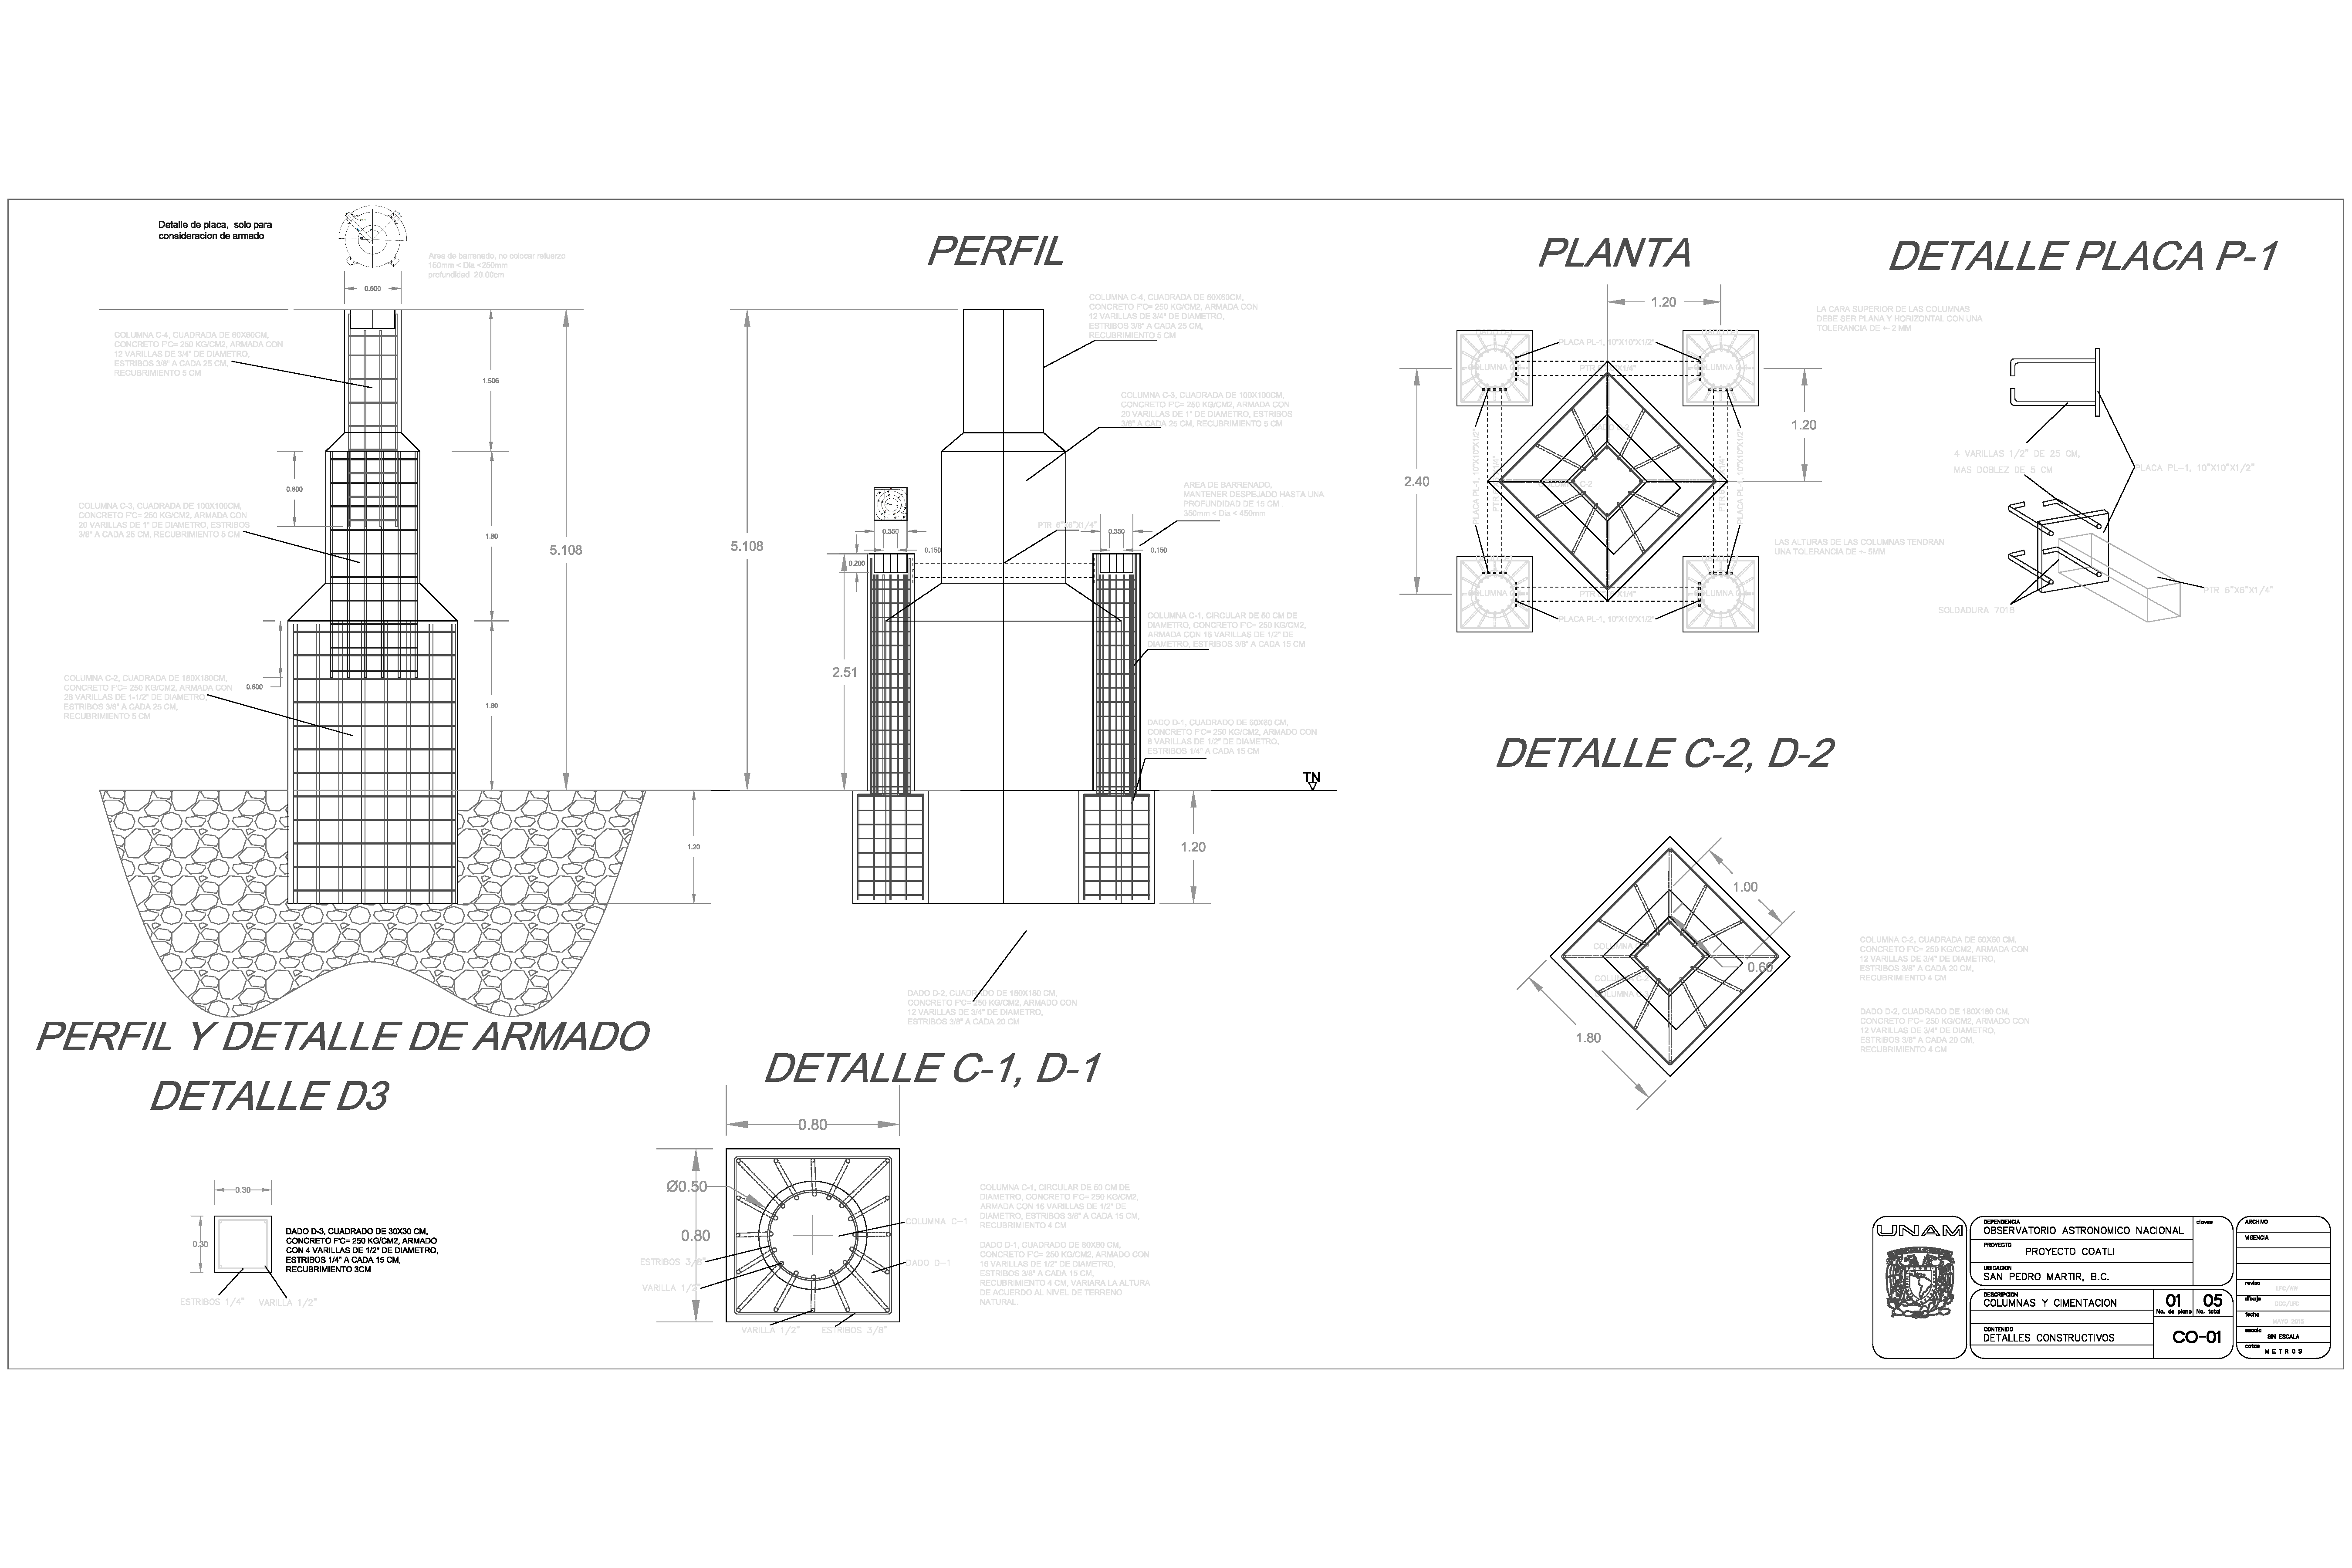
\includegraphics[height=0.95\linewidth,angle=90]{figures/buildings-coatli-drawing-2015-1.pdf}
\end{center}
\caption{{\projectname} original 2015 design drawing (1 of 5).}
\label{figure:buildings-drawing-2015-1}
\end{figure*}

\begin{figure*}
\begin{center}
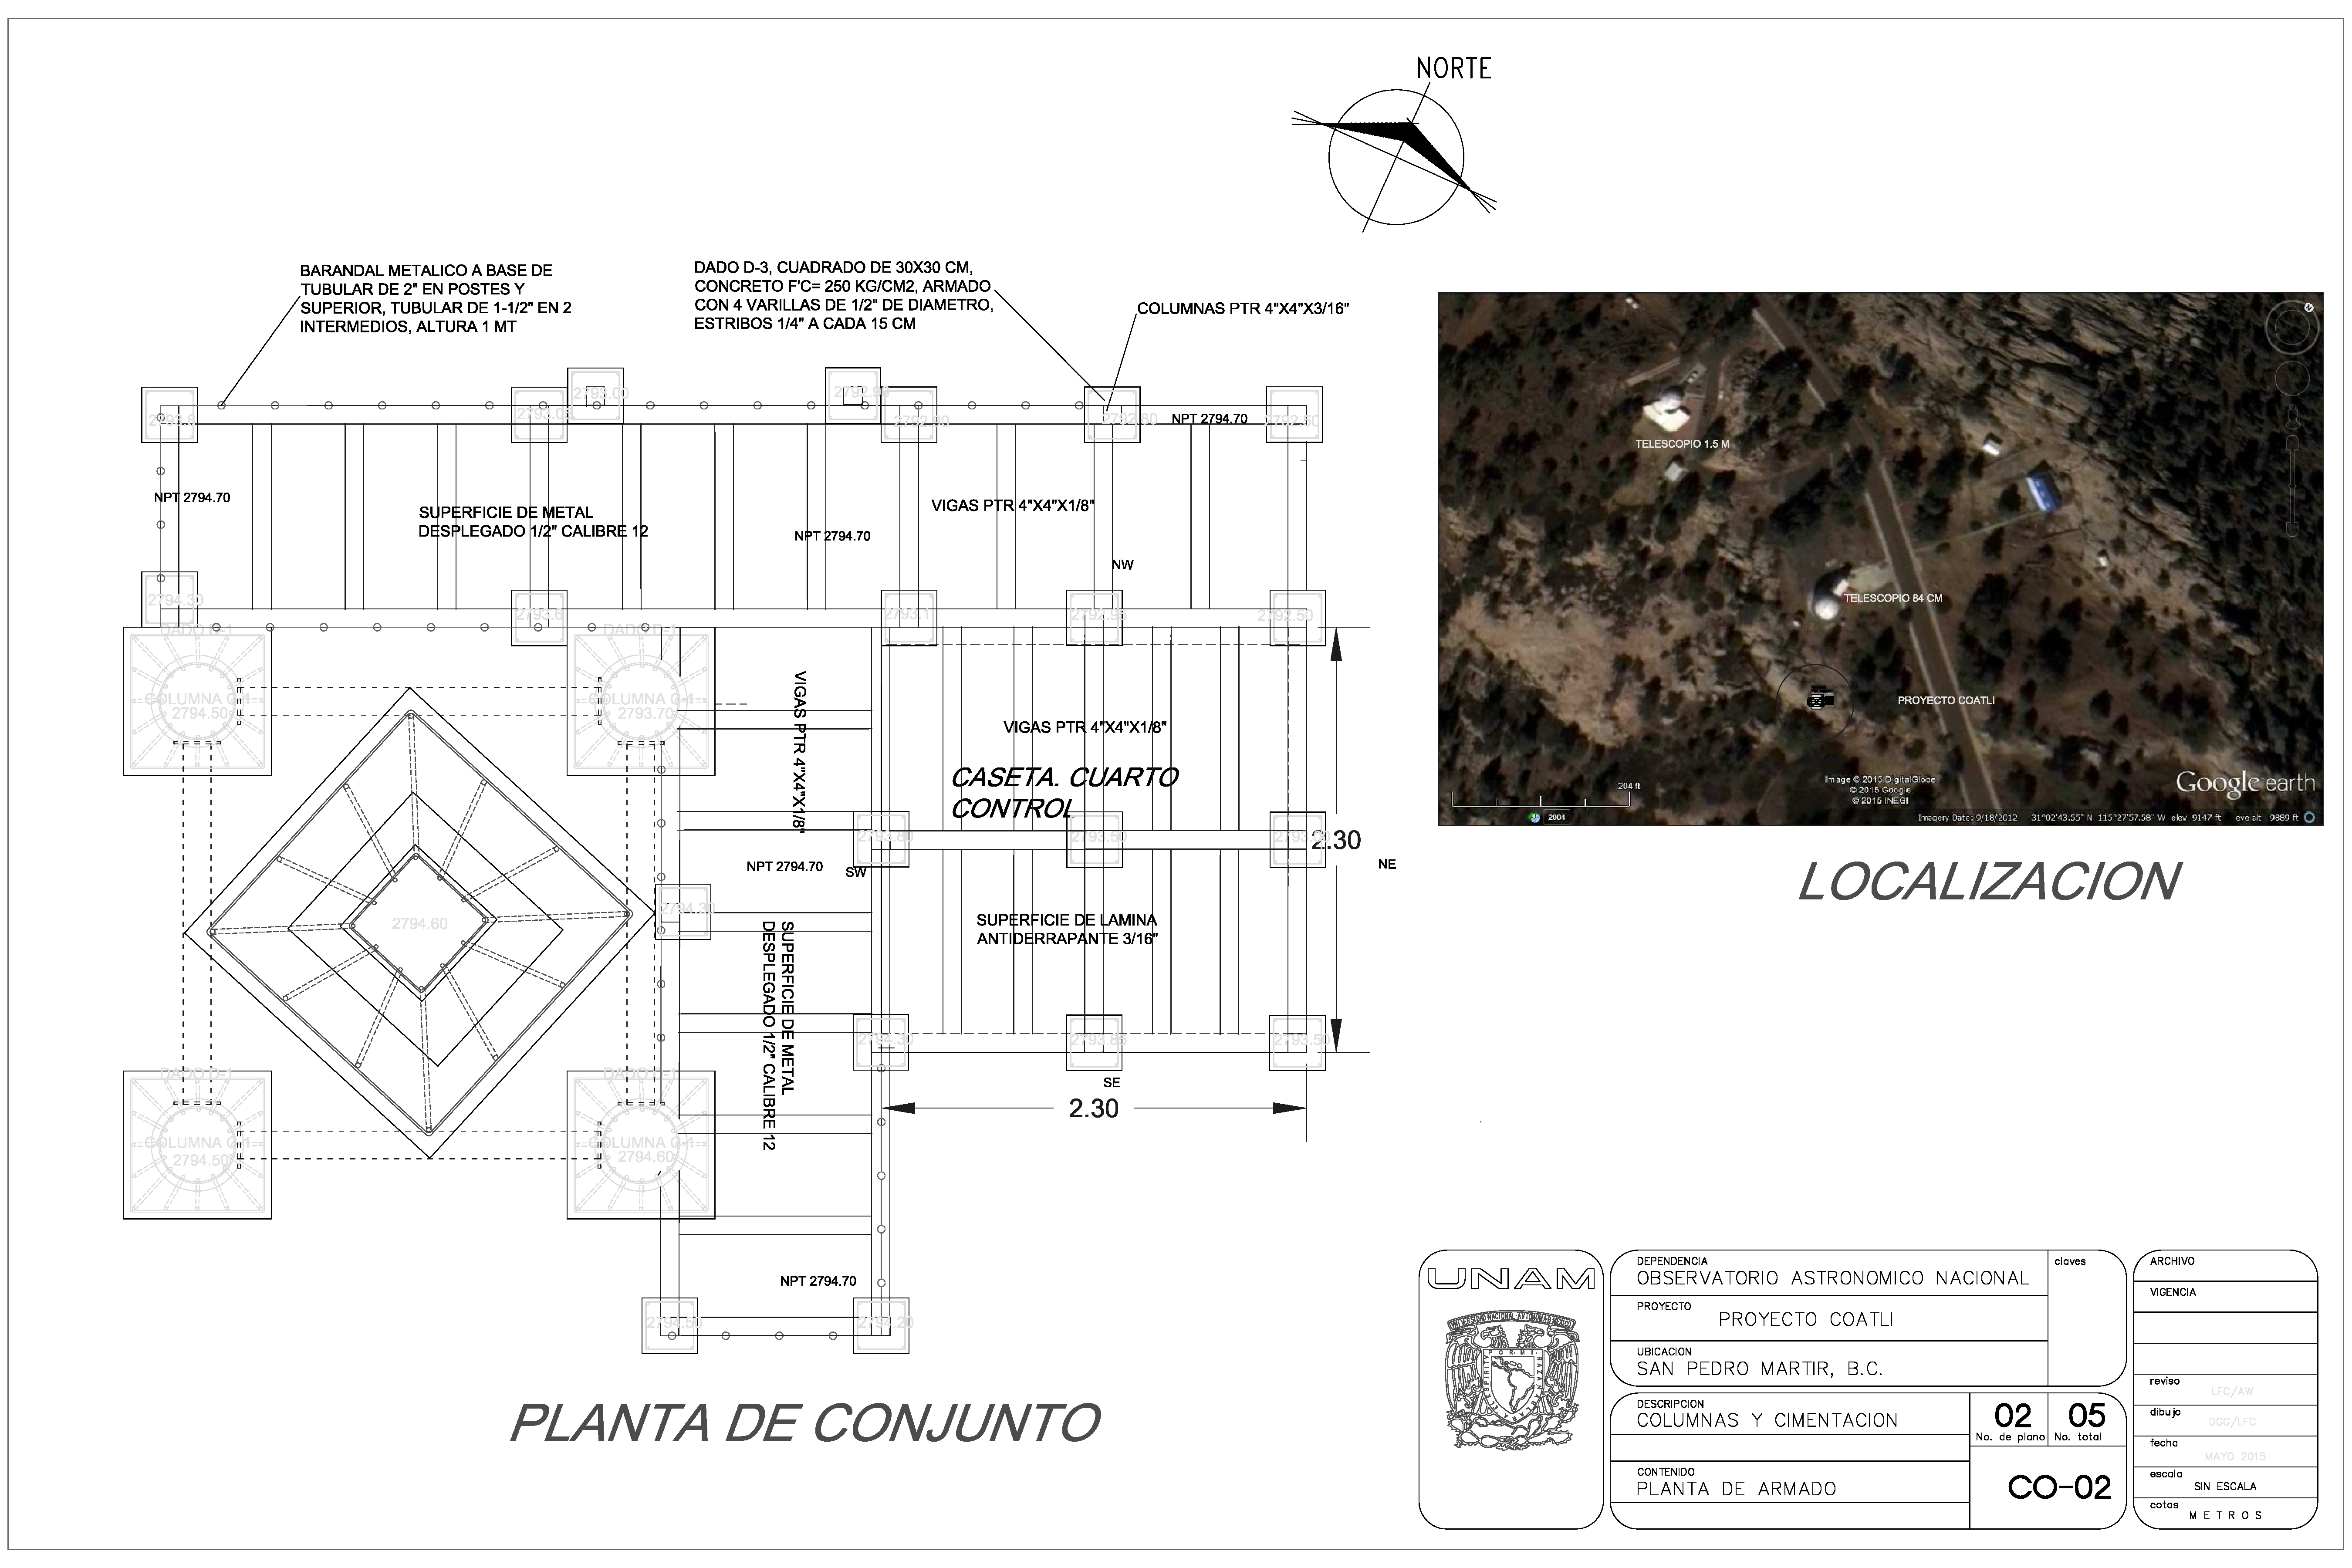
\includegraphics[height=0.95\linewidth,angle=90]{figures/buildings-coatli-drawing-2015-2.pdf}
\end{center}
\caption{{\projectname} original 2015 design drawing (2 of 5). The actual stairs turn by 90 degrees to descend towards the 84-cm building. See Figure~\ref{figure:buildings-drawing-2015-3}.}
\label{figure:buildings-drawing-2015-2}
\end{figure*}

\begin{figure*}
\begin{center}
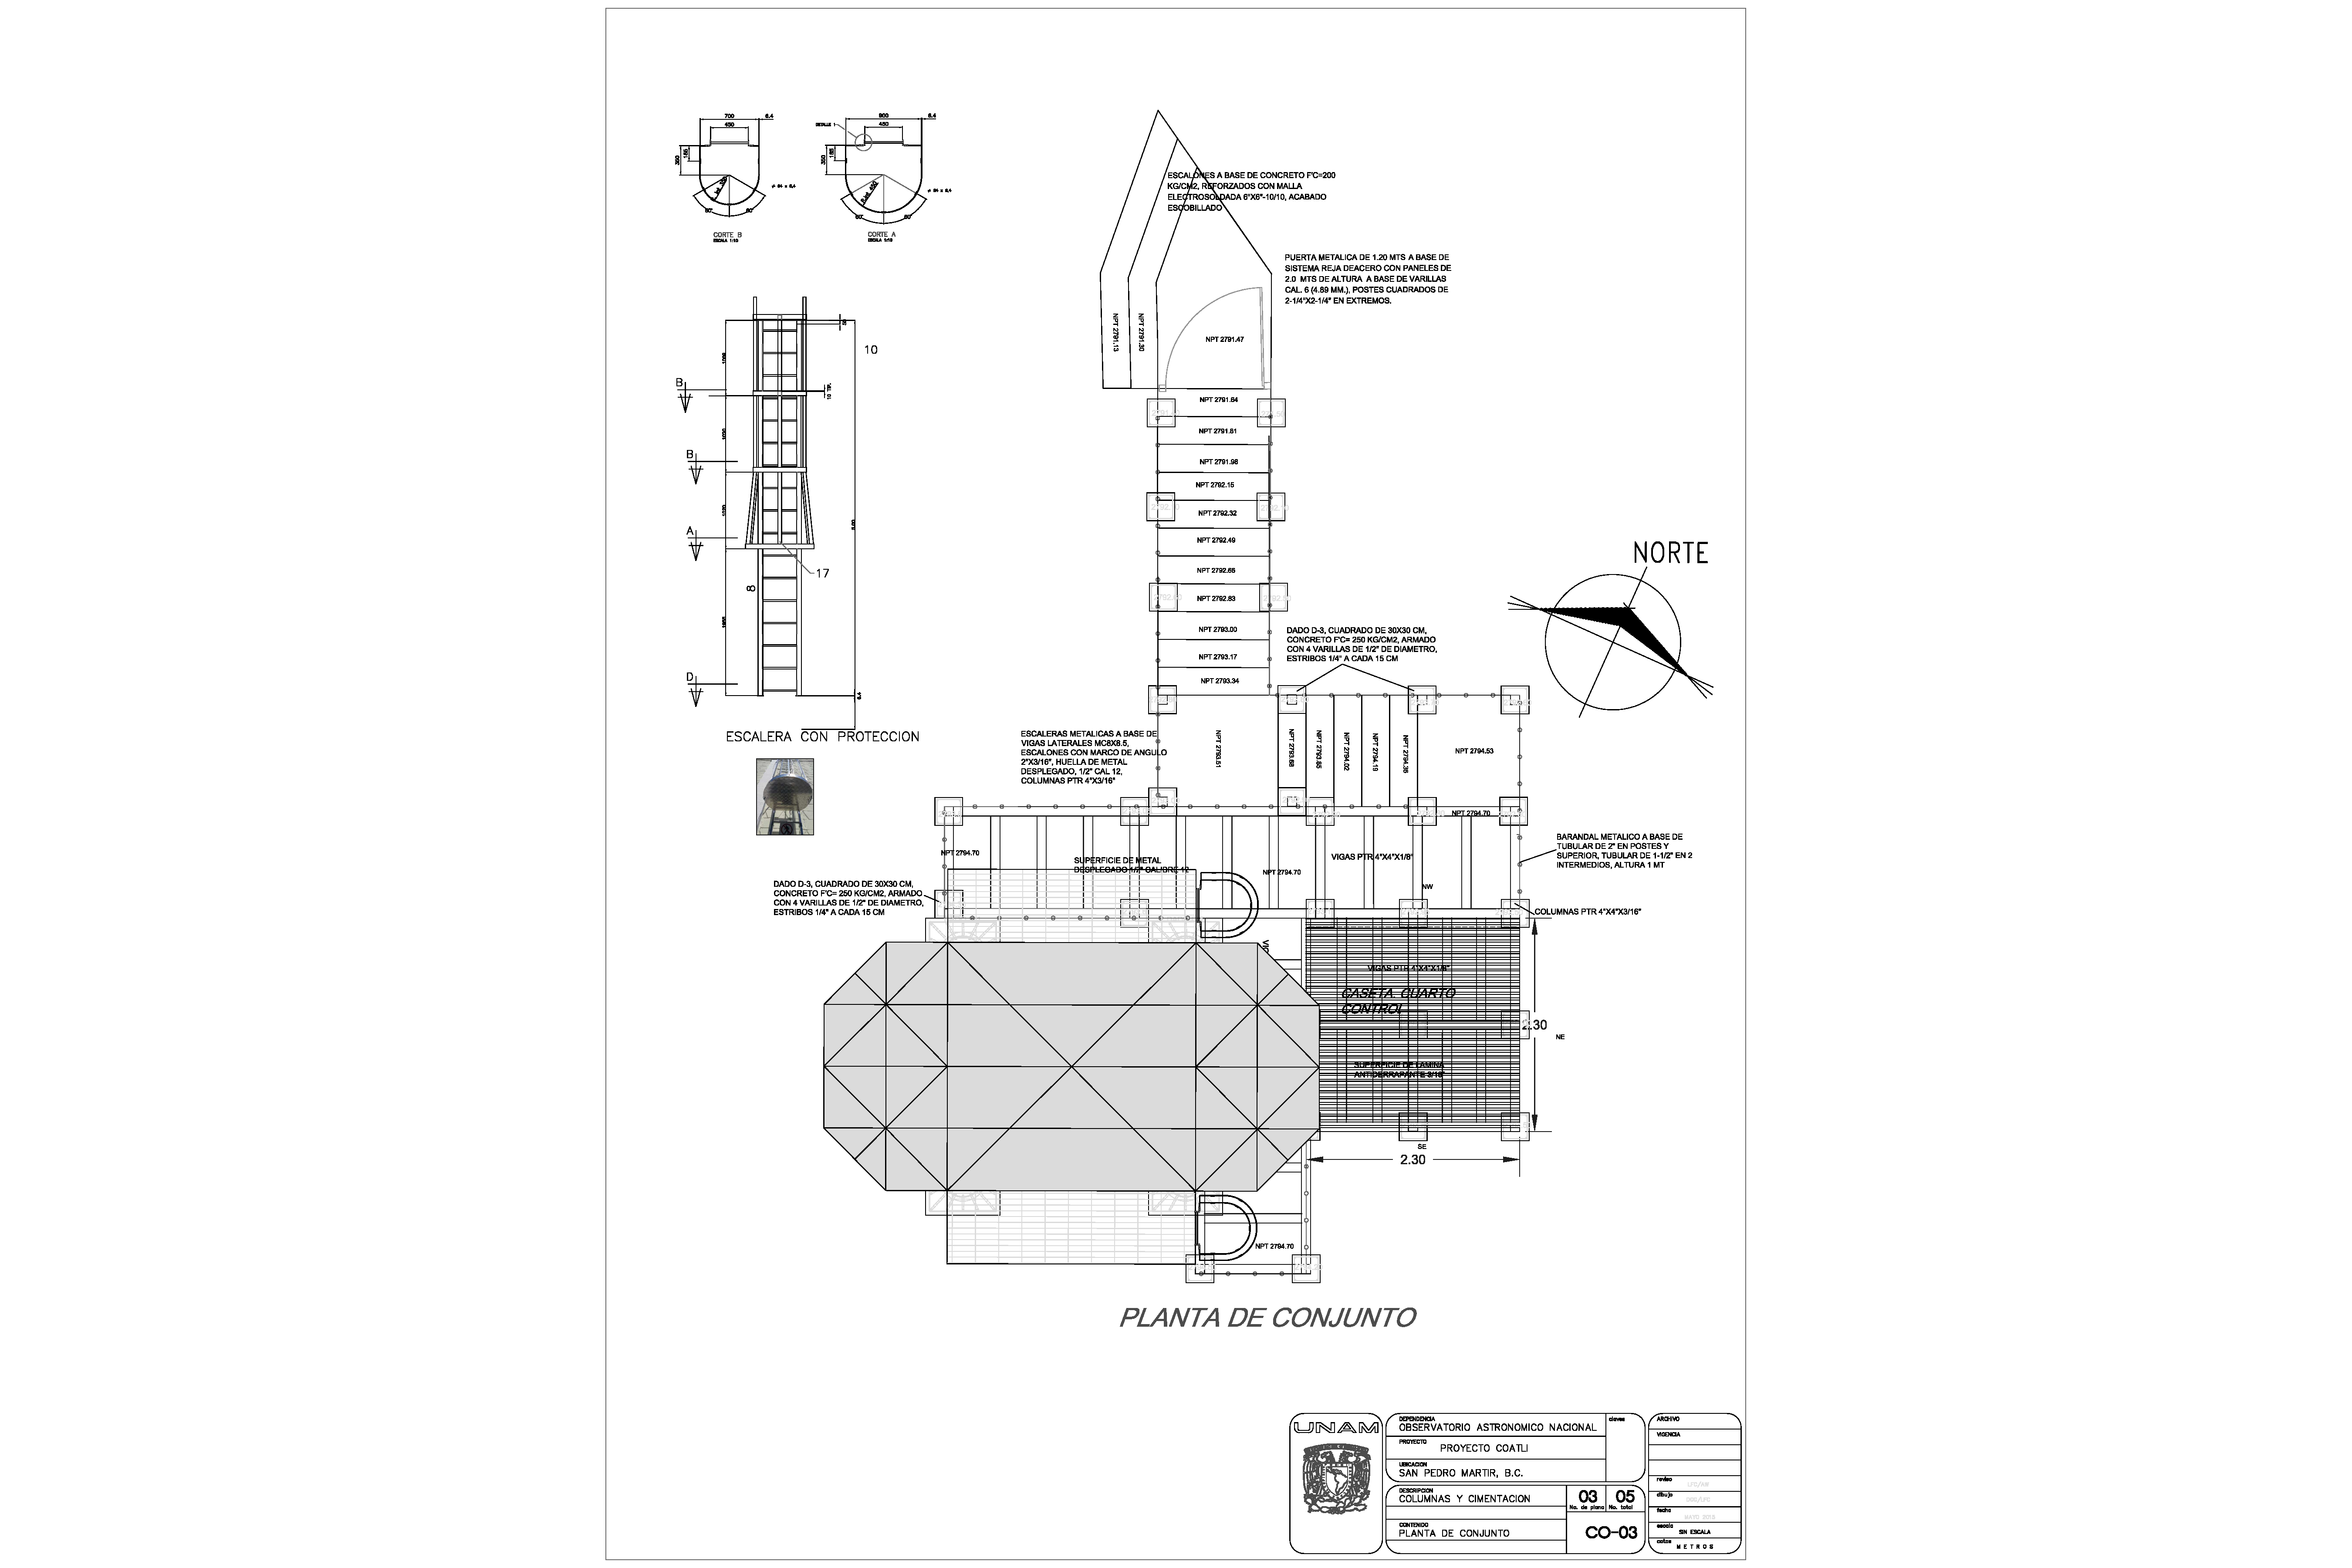
\includegraphics[width=0.95\linewidth]{figures/buildings-coatli-drawing-2015-3.pdf}
\end{center}
\caption{{\projectname} original 2015 design drawing (3 of 5).}
\label{figure:buildings-drawing-2015-3}
\end{figure*}

\begin{figure*}
\begin{center}
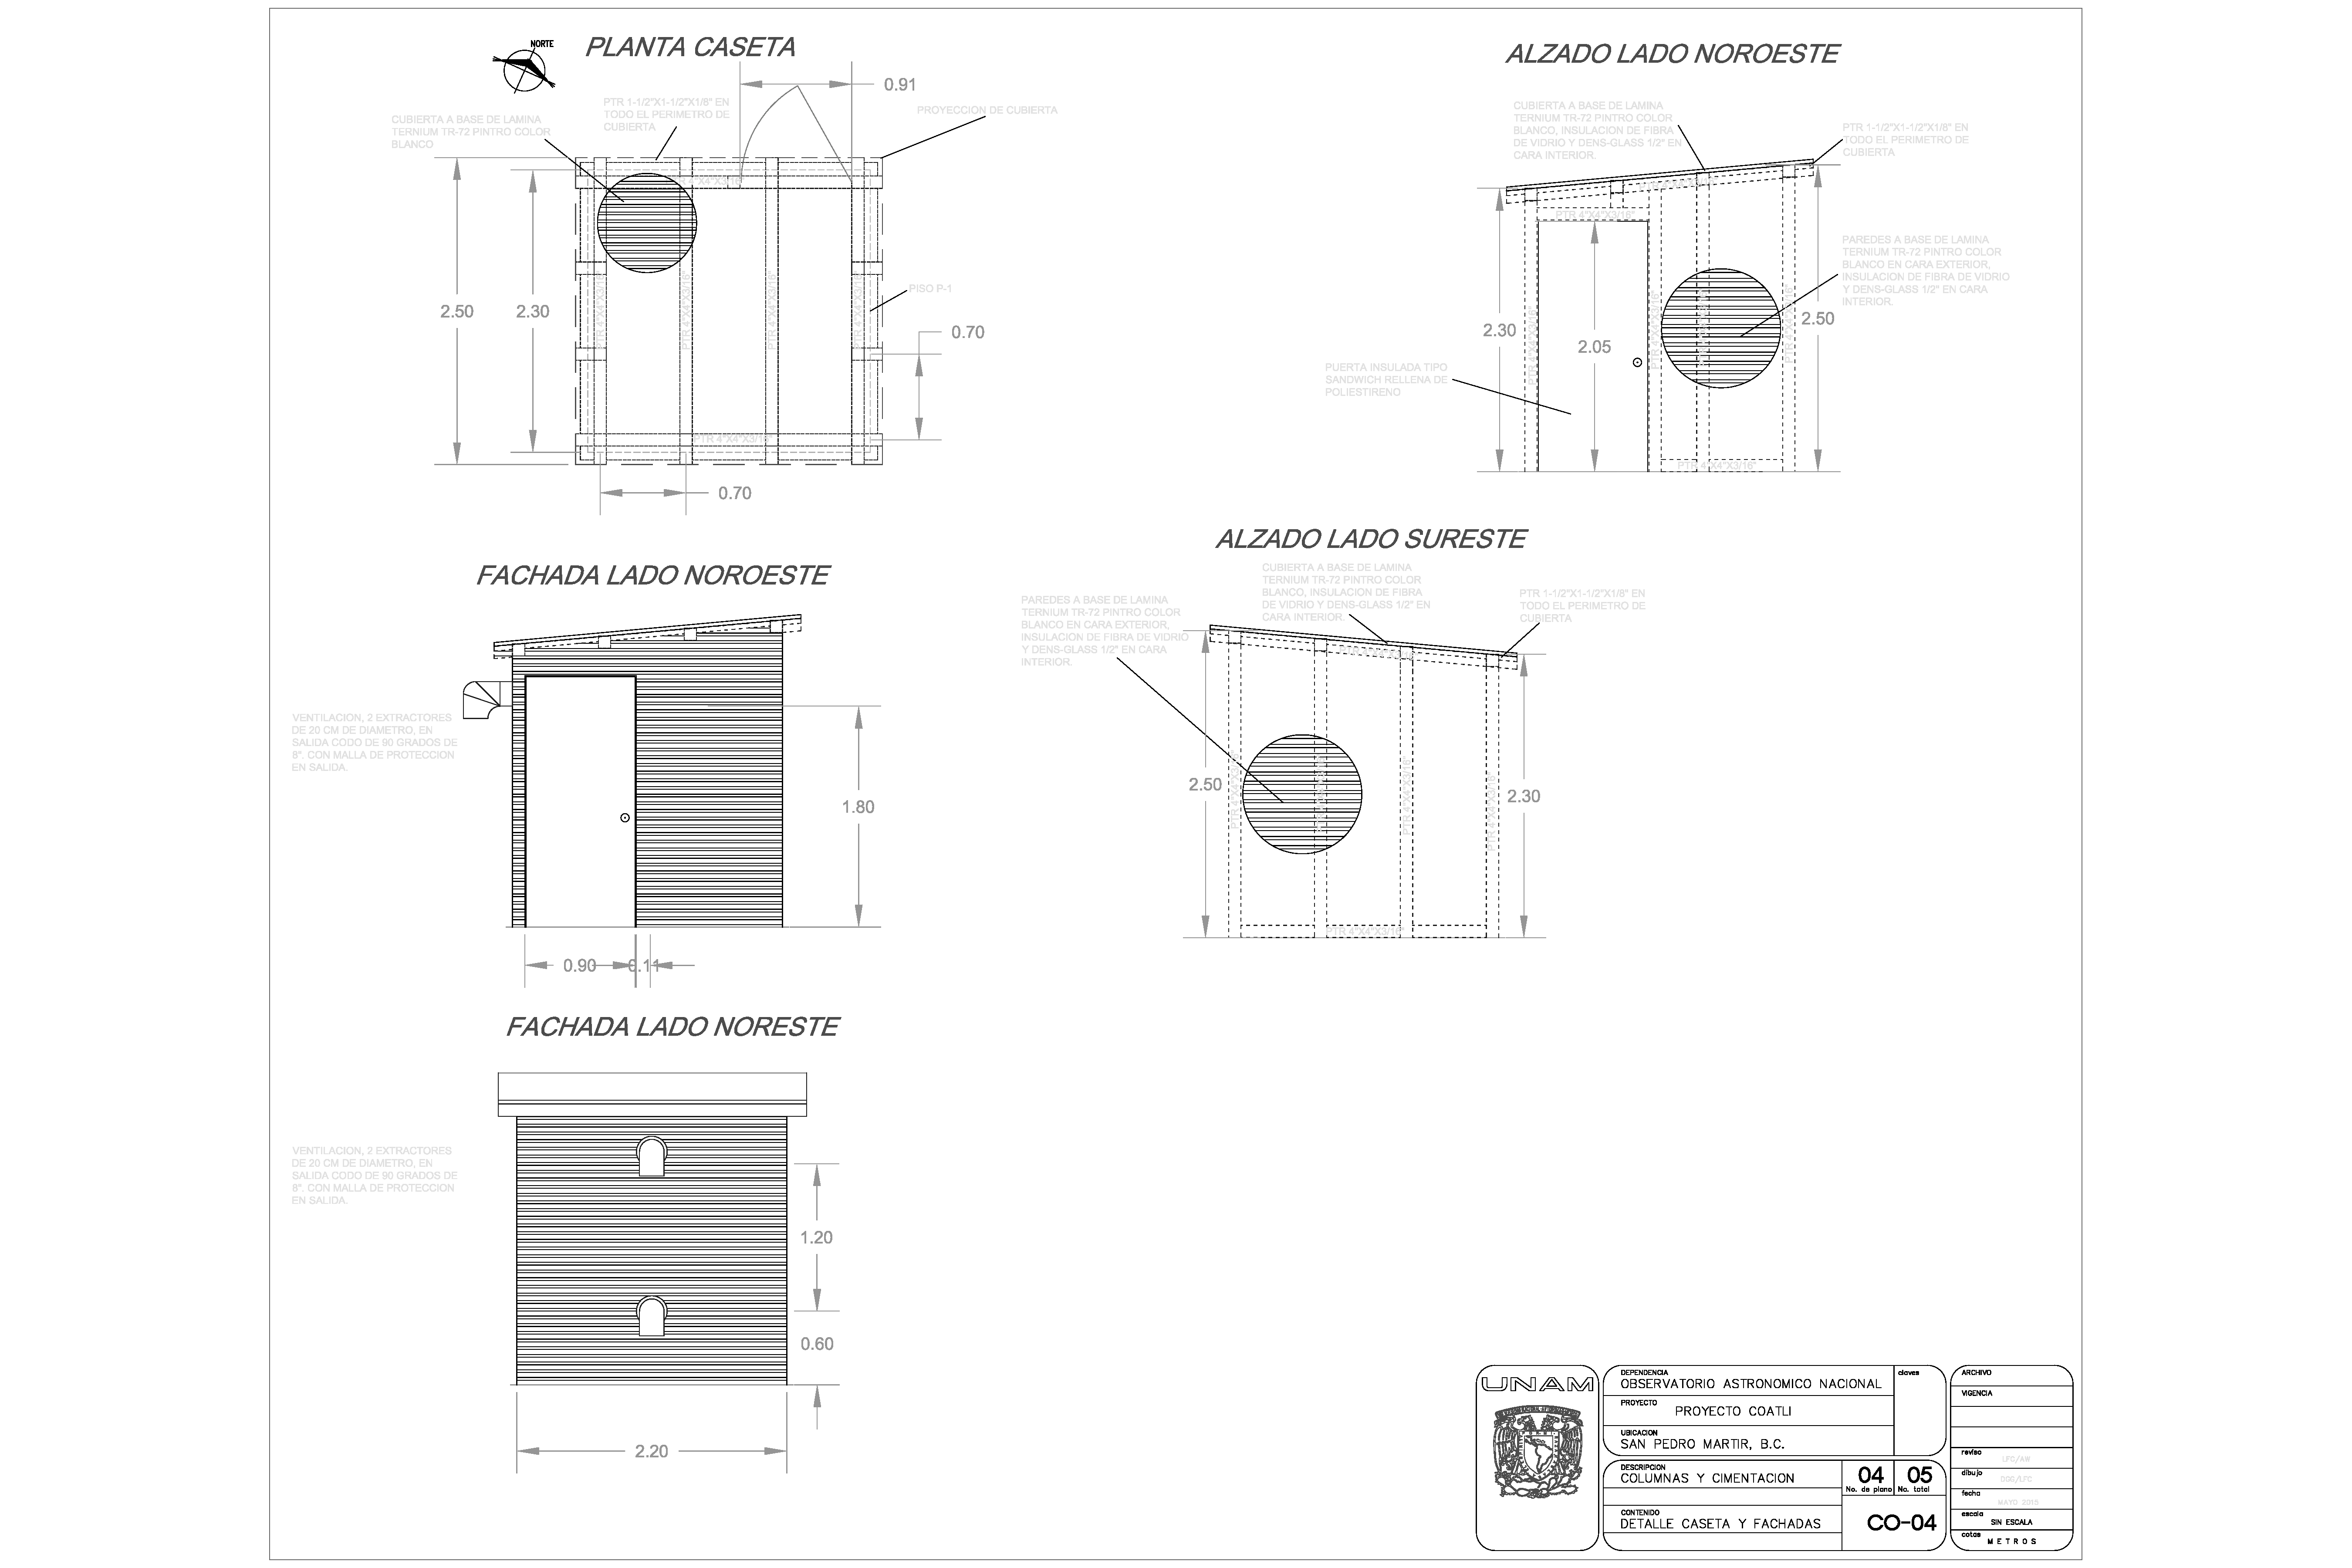
\includegraphics[height=0.95\linewidth,angle=90]{figures/buildings-coatli-drawing-2015-4.pdf}
\end{center}
\caption{{\projectname} original 2015 design drawing (4 of 5).}
\label{figure:buildings-drawing-2015-4}
\end{figure*}

\begin{figure*}
\begin{center}
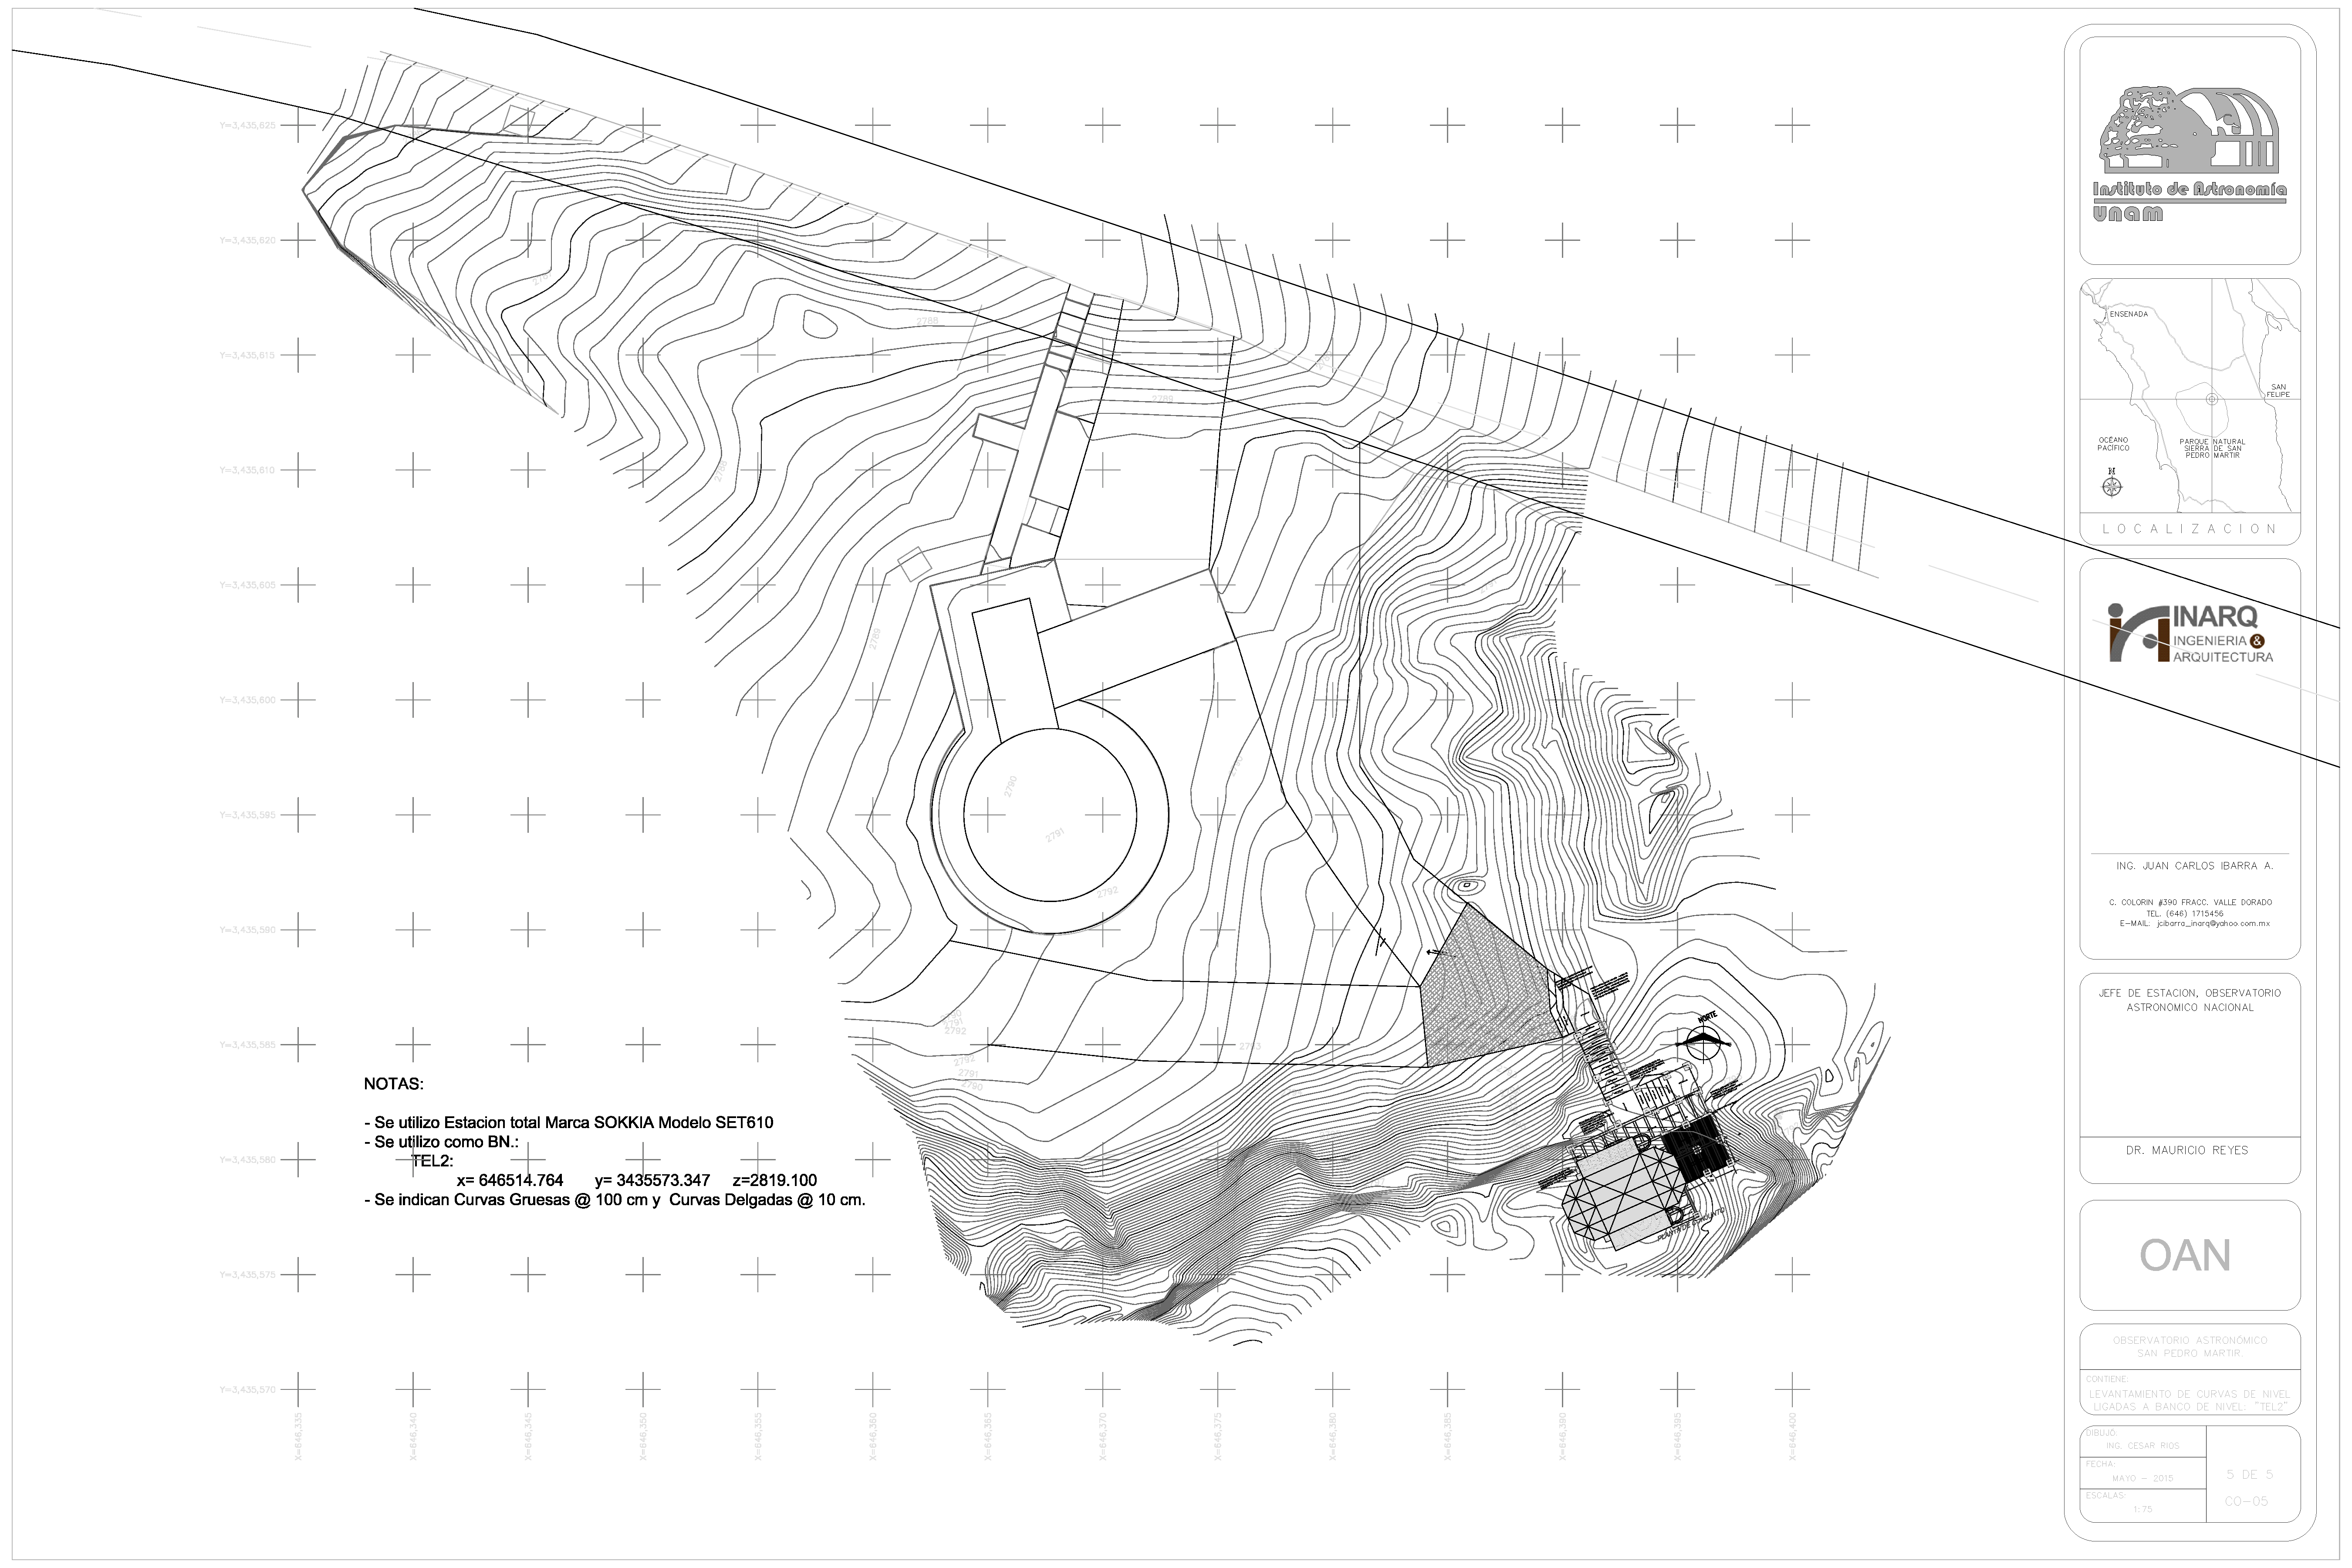
\includegraphics[height=0.95\linewidth,angle=90]{figures/buildings-coatli-drawing-2015-5.pdf}
\end{center}
\caption{{\projectname} original 2018 design drawing (5 of 5).}
\label{figure:buildings-drawing-2015-5}
\end{figure*}

\begin{figure*}
\begin{center}
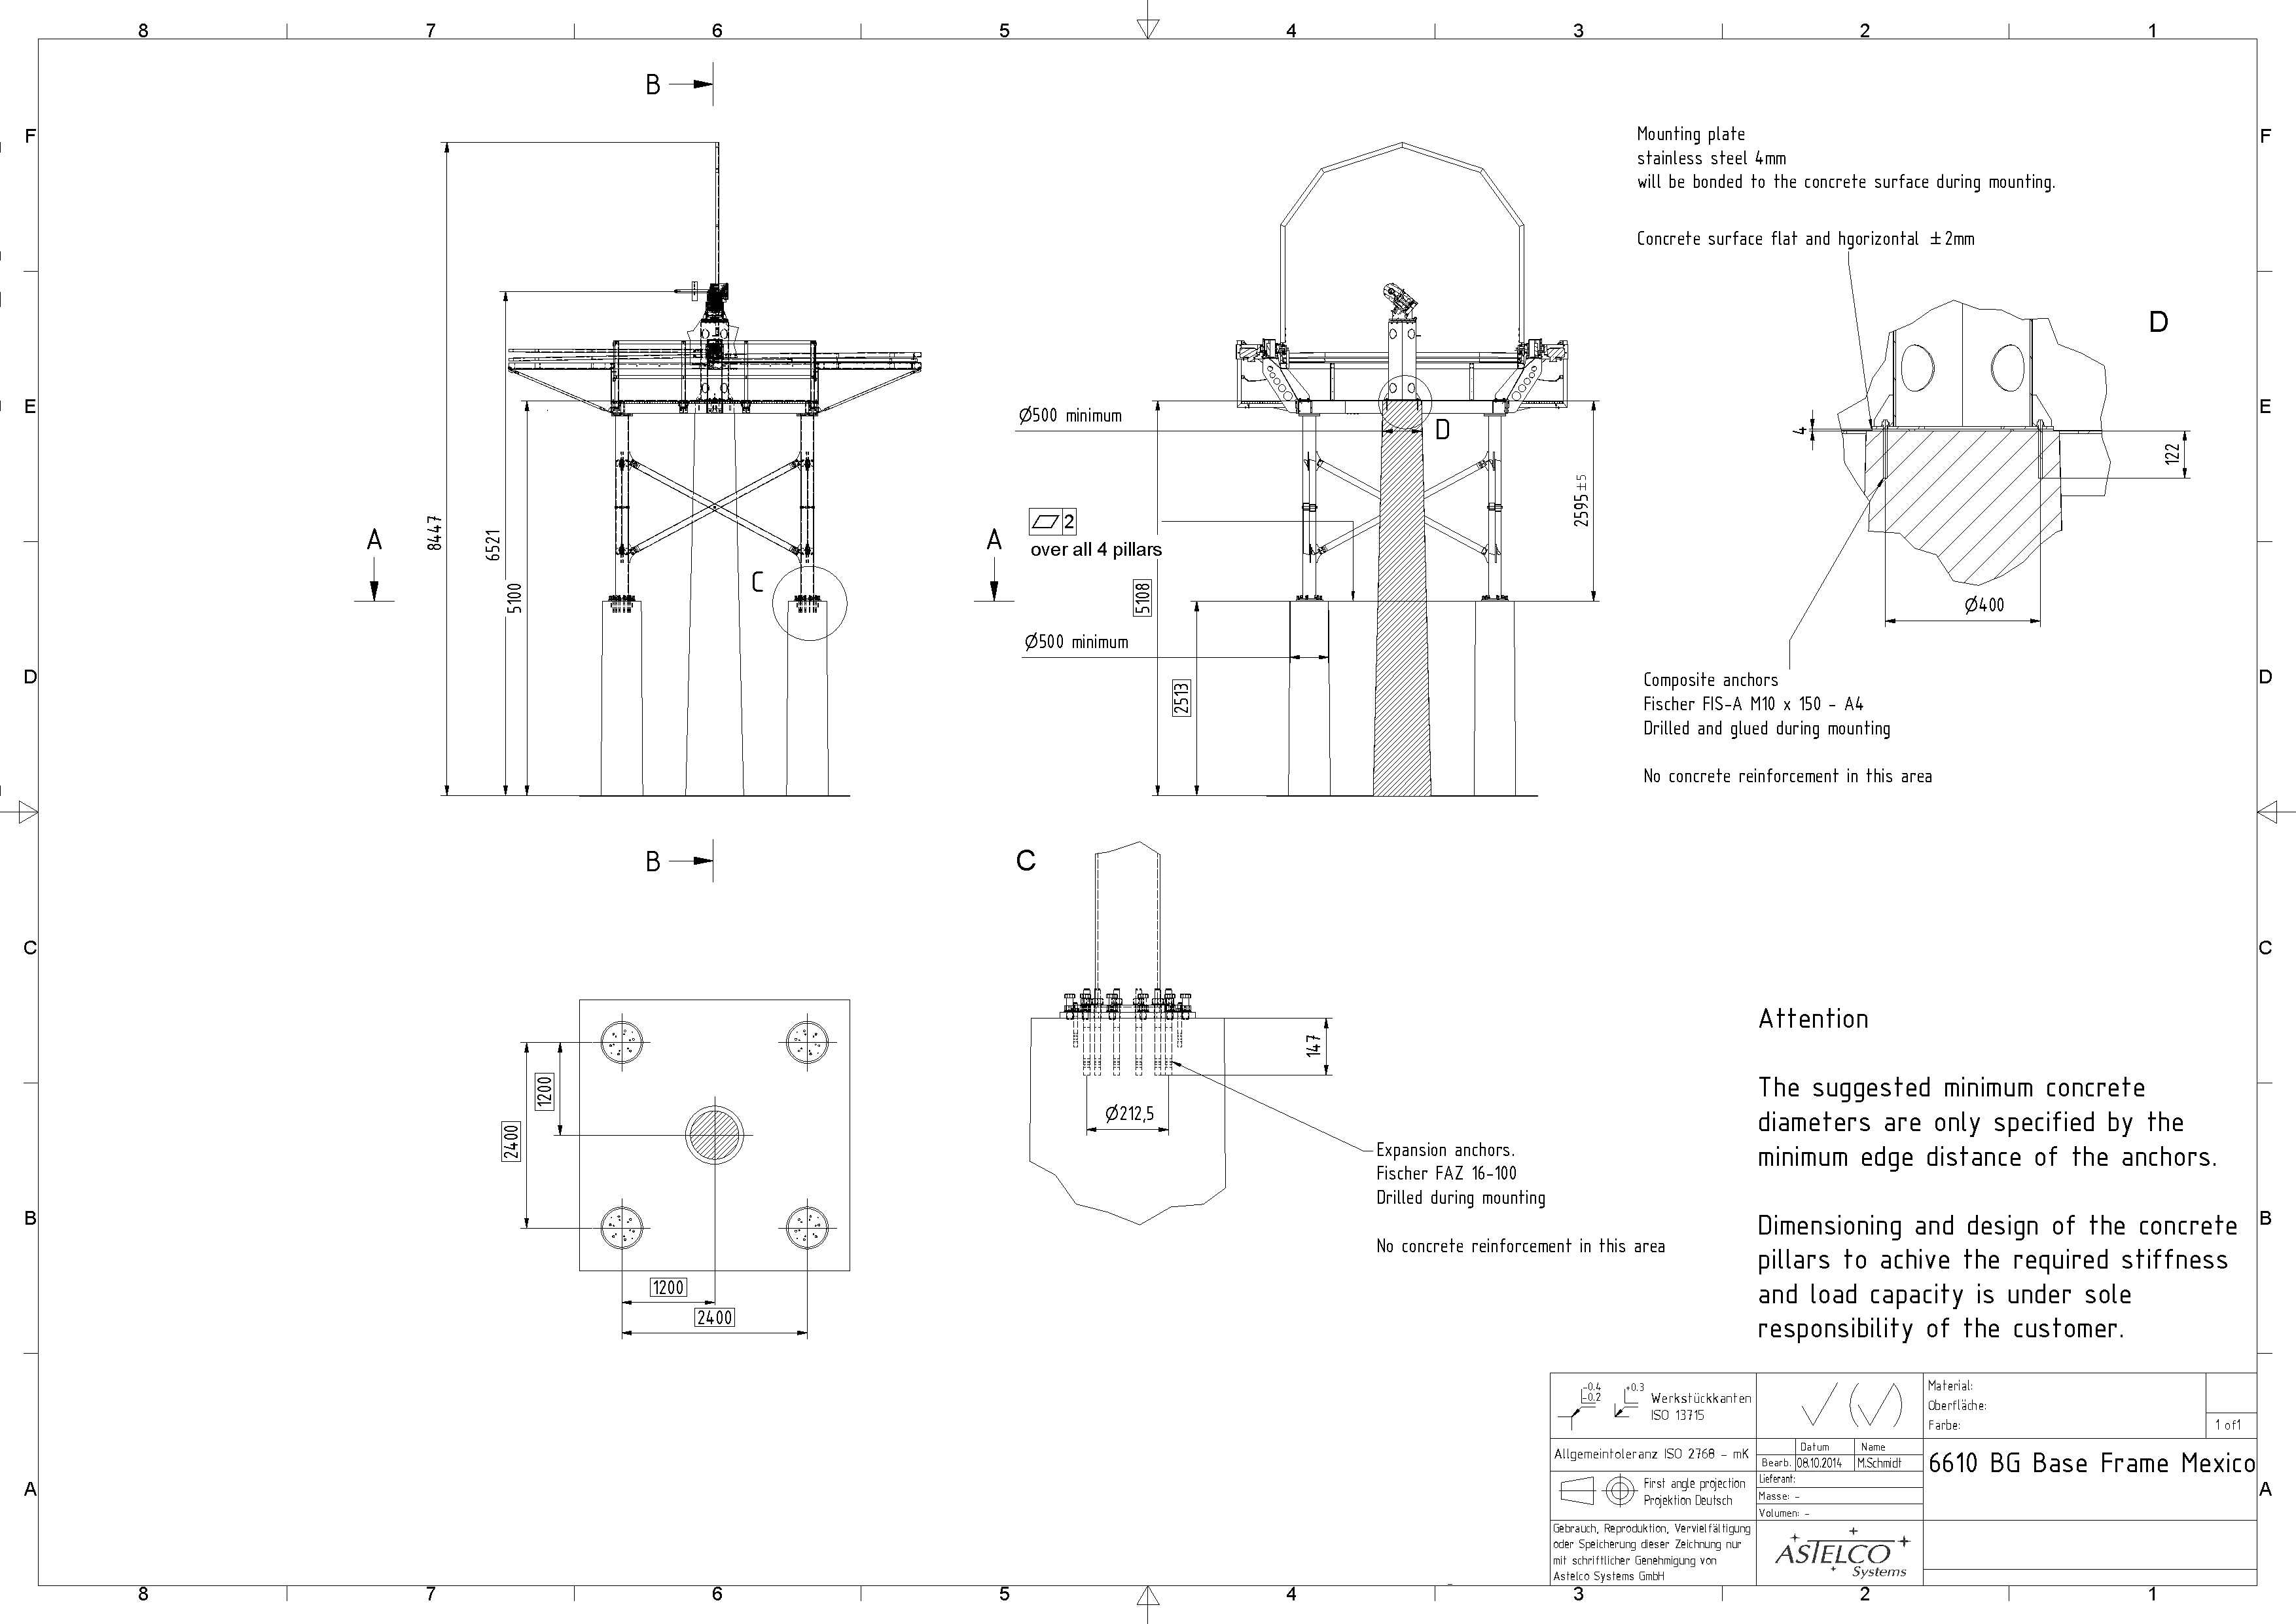
\includegraphics[height=0.95\linewidth,angle=90]{figures/buildings-coatli-astelco-enclosure-drawing-6610}
\end{center}
\caption{{\projectname} ASTELCO Platform and Telescope Pillar.}
\label{figure:buildings-drawing-astelco}
\end{figure*}

\begin{figure*}
\begin{center}
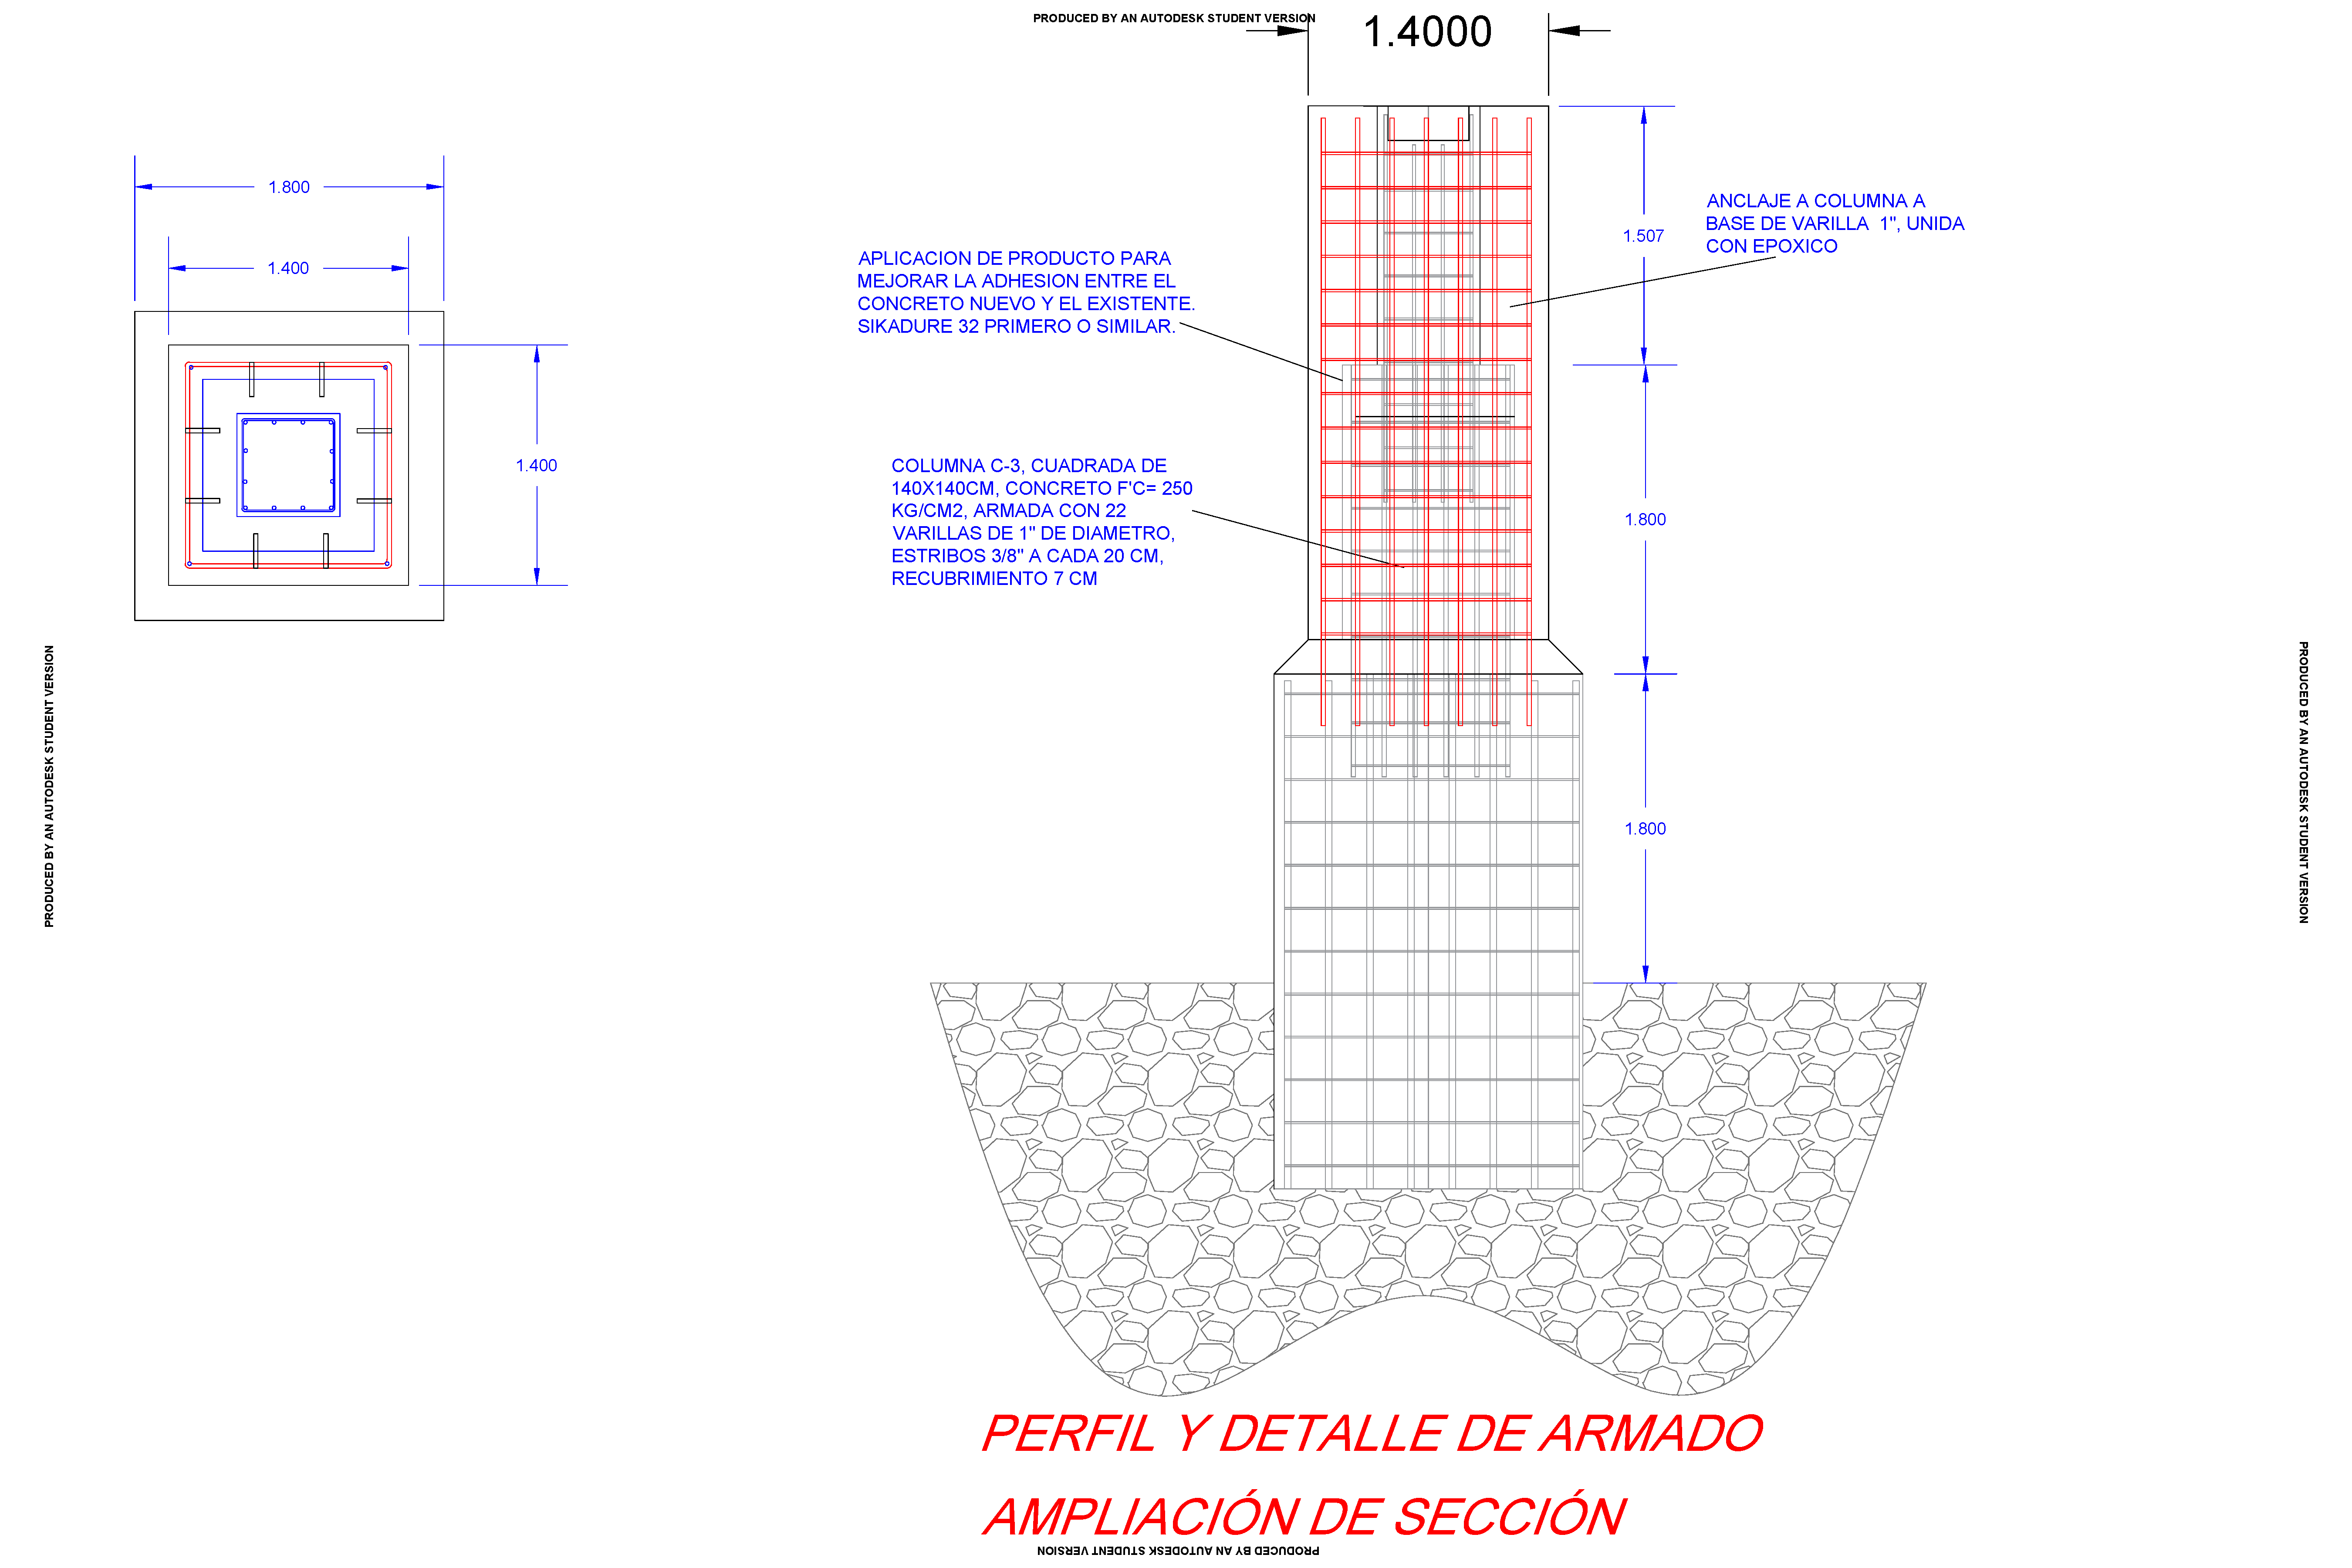
\includegraphics[height=0.95\linewidth,angle=90]{figures/buildings-coatli-drawing-2018-1.pdf}
\end{center}
\caption{{\projectname} Modified 2018 design drawing (1 of 3).}
\label{figure:buildings-drawing-2018-1}
\end{figure*}

\begin{figure*}
\begin{center}
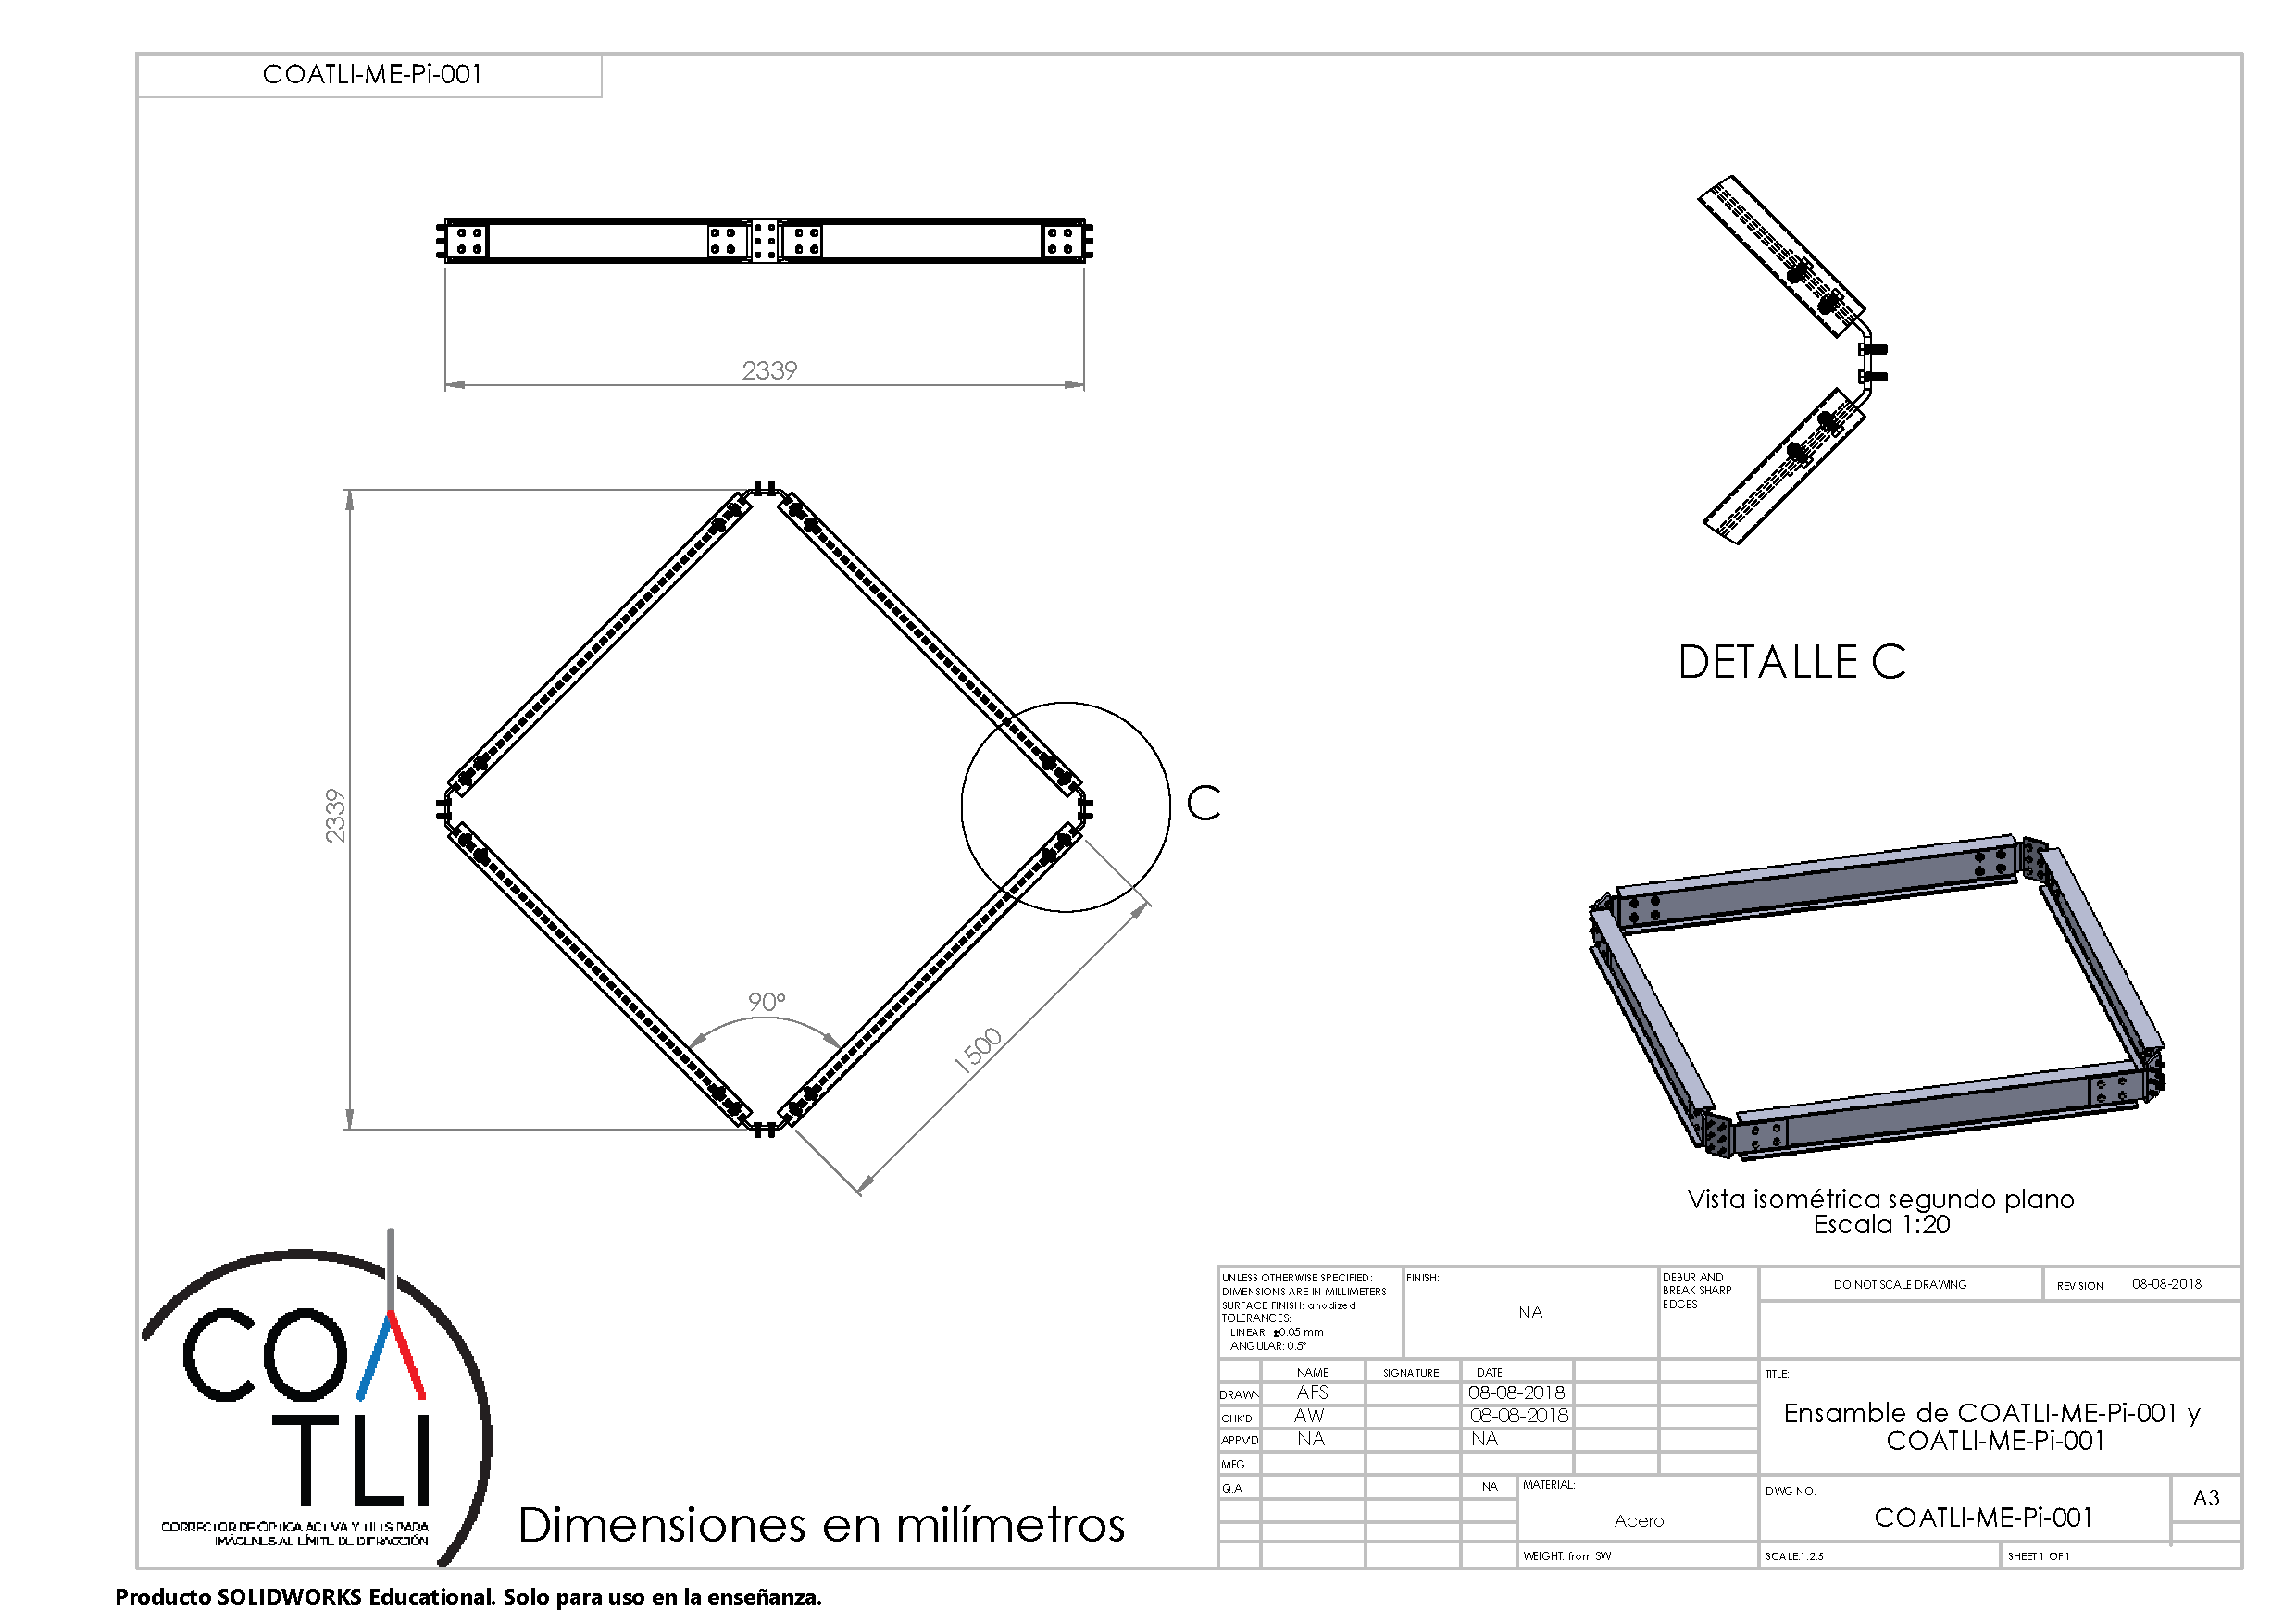
\includegraphics[height=0.95\linewidth,angle=90]{figures/buildings-coatli-drawing-2018-2.pdf}
\end{center}
\caption{{\projectname} Modified 2018 design drawing (2 of 3).}
\label{figure:buildings-drawing-2018-2}
\end{figure*}

\begin{figure*}
\begin{center}
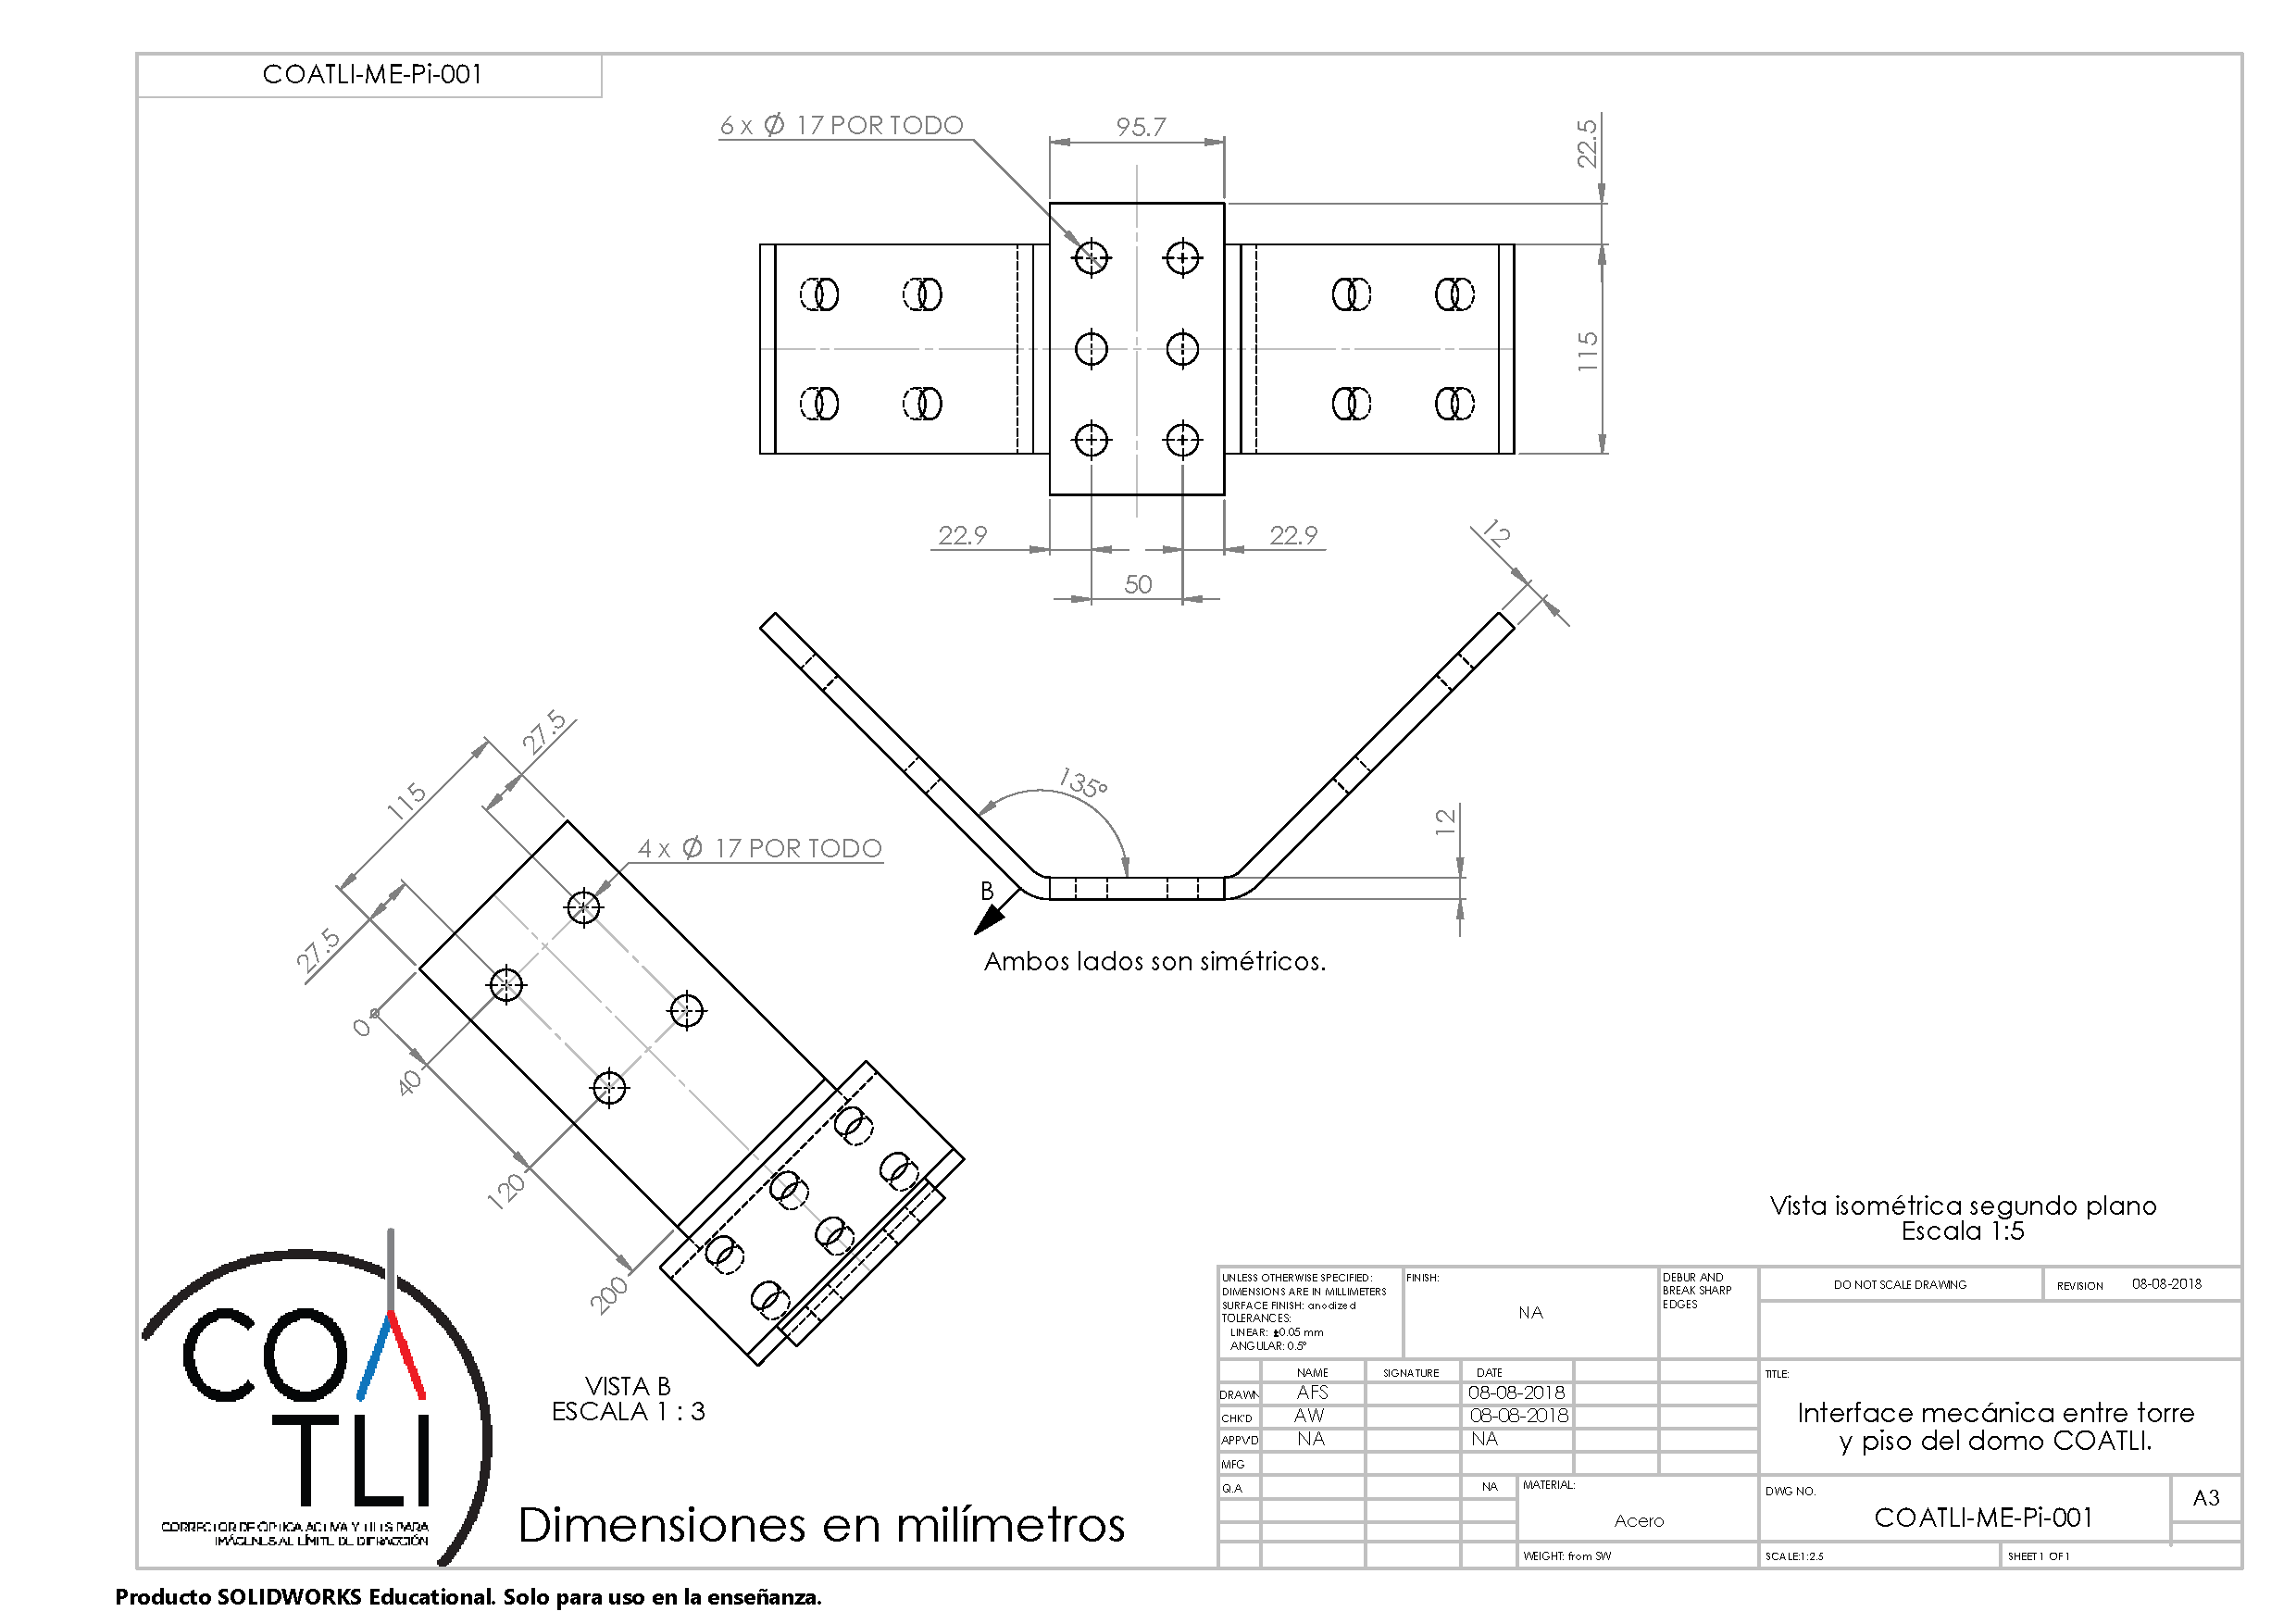
\includegraphics[height=0.95\linewidth,angle=90]{figures/buildings-coatli-drawing-2018-3.pdf}
\end{center}
\caption{{\projectname} Modified 2018 design drawing (3 of 3).}
\label{figure:buildings-drawing-2018-3}
\end{figure*}
\fi

\ifddoti

The shed, access, and tower are constructed on open space to the north of the 84-cm building. The buildings and structures were constructed in 2016 and the enclosure installed in 2017.

Figures~\ref{figure:buildings-drawing-2016-1} to \ref{figure:buildings-drawing-2016-3} show the 2016 design drawings for the shed, access staircase and walkways, and the concrete columns that support the platform and telescope. The original design was largely based on that of COATLI, but with simplifications for the easier site and a slightly different telescope column. The DDOTI telescope column extended 40 cm above the platform floor (the COATLI column is flush with the platform floor) to reduce the height of the steel pier and increase its stability. Figure  \ref{figure:buildings-drawing-astelco} shows the ASTELCO ARTS platform and the ASTELCO steel pillar mounted on the concrete columns (although this drawing is for COATLI, the DDOTI enclosure is identical except for the perforation in the platform floor). Figure  \ref{figure:buildings-drawing-astelco-pier} shows the ASTELCO pier. The center of rotation of the mount axes is about 6.5 meters above the ground level.

During the summer of 2016, the design of the telescope column was changed without this change being adequately communicated to the project. The telescope concrete column  originally was designed with three parts, each square in cross section and tapering from 1.8, 1.2, and 0.6 meters to a side, like the COATLI column. The design was changed so that the middle and upper sections were uniformly 1.0 meters to a side (although some erroneous vestiges of the original column remain in Figures~\ref{figure:buildings-drawing-2016-1}). Fortunately, this change was caught in time to allow the platform to be modified.

The original design was intended to be oriented with the long-axis of the enclosure aligned with geographic N-S (see Figure~\ref{figure:buildings-drawing-2016-2}). However, when the site was laid out, the surveyor made a sign error in the magnetic deviation. Instead of being aligned with geographic north (11 degrees west of magnetic north) the structures were aligned 22 degrees east of geographic north (11 degrees east of magnetic north). This error was not detected until the lower part of the telescope column had been poured. Fortunately, the column and enclosure could still accommodate the pier, mount, and telescopes.

\begin{figure*}
\begin{center}
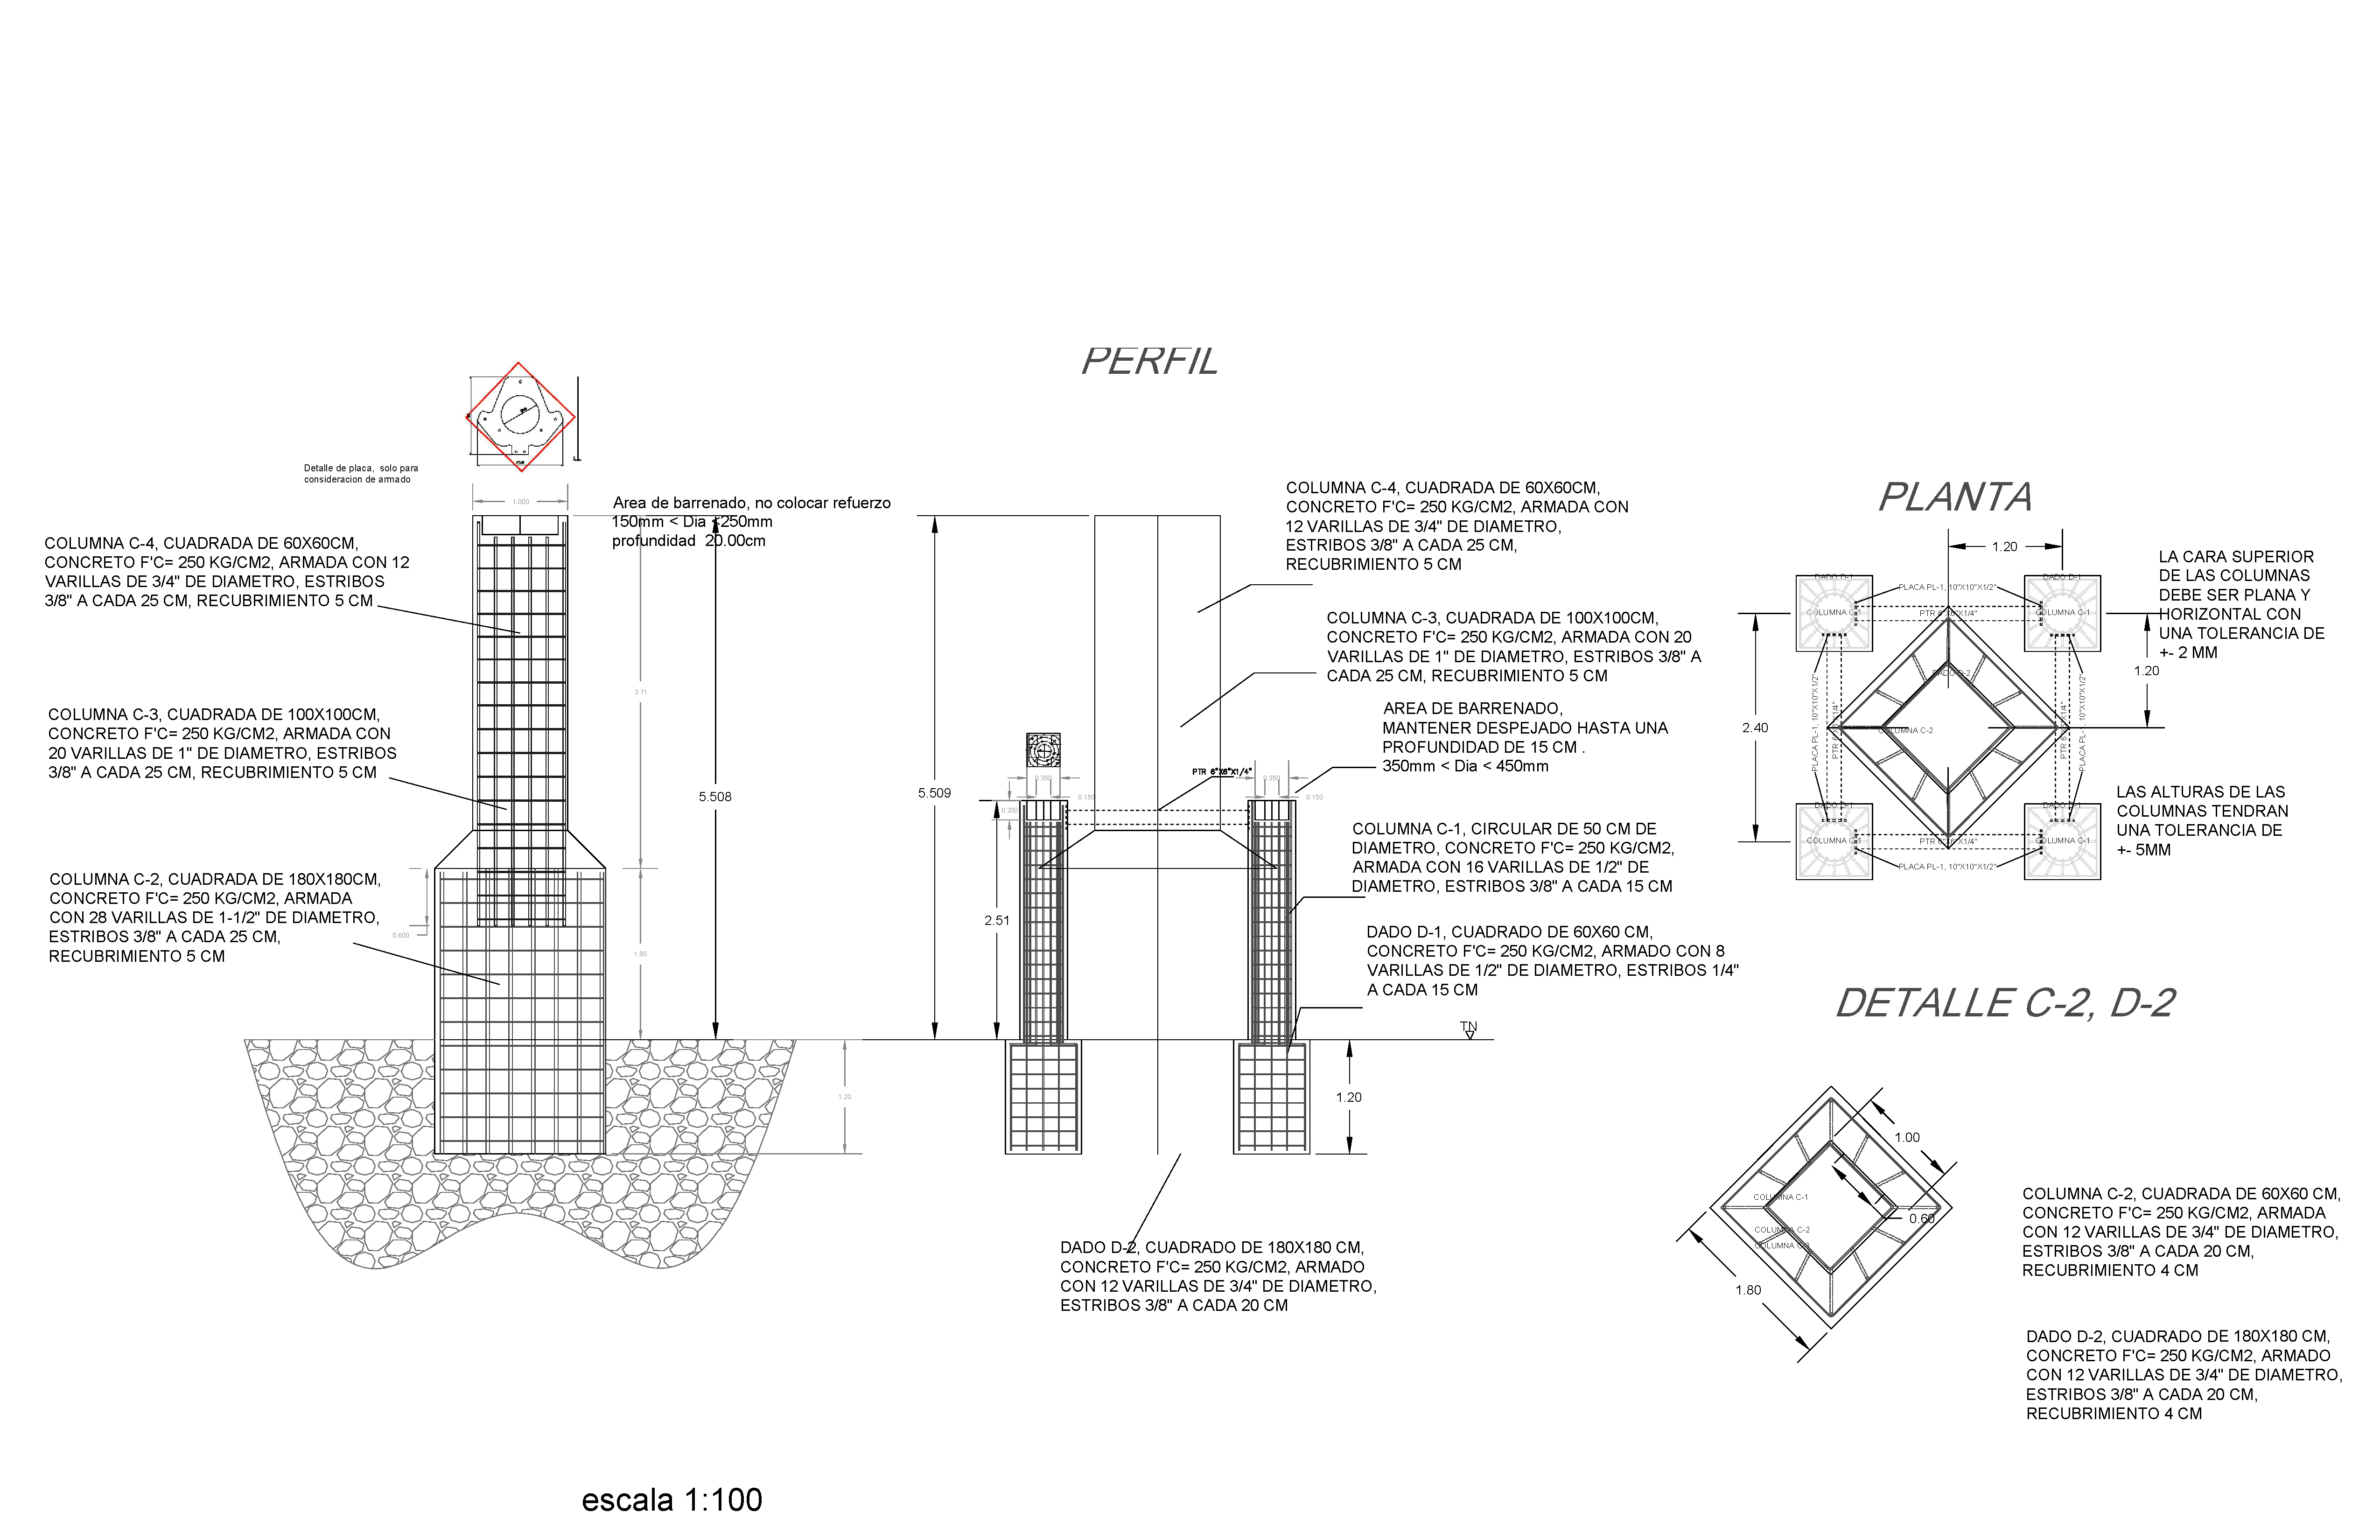
\includegraphics[height=0.95\linewidth,angle=90]{figures/buildings-ddoti-drawing-2016-1.pdf}
\end{center}
\caption{{\projectname} original 2016 design drawing (1 of 3).}
\label{figure:buildings-drawing-2016-1}
\end{figure*}

\begin{figure*}
\begin{center}
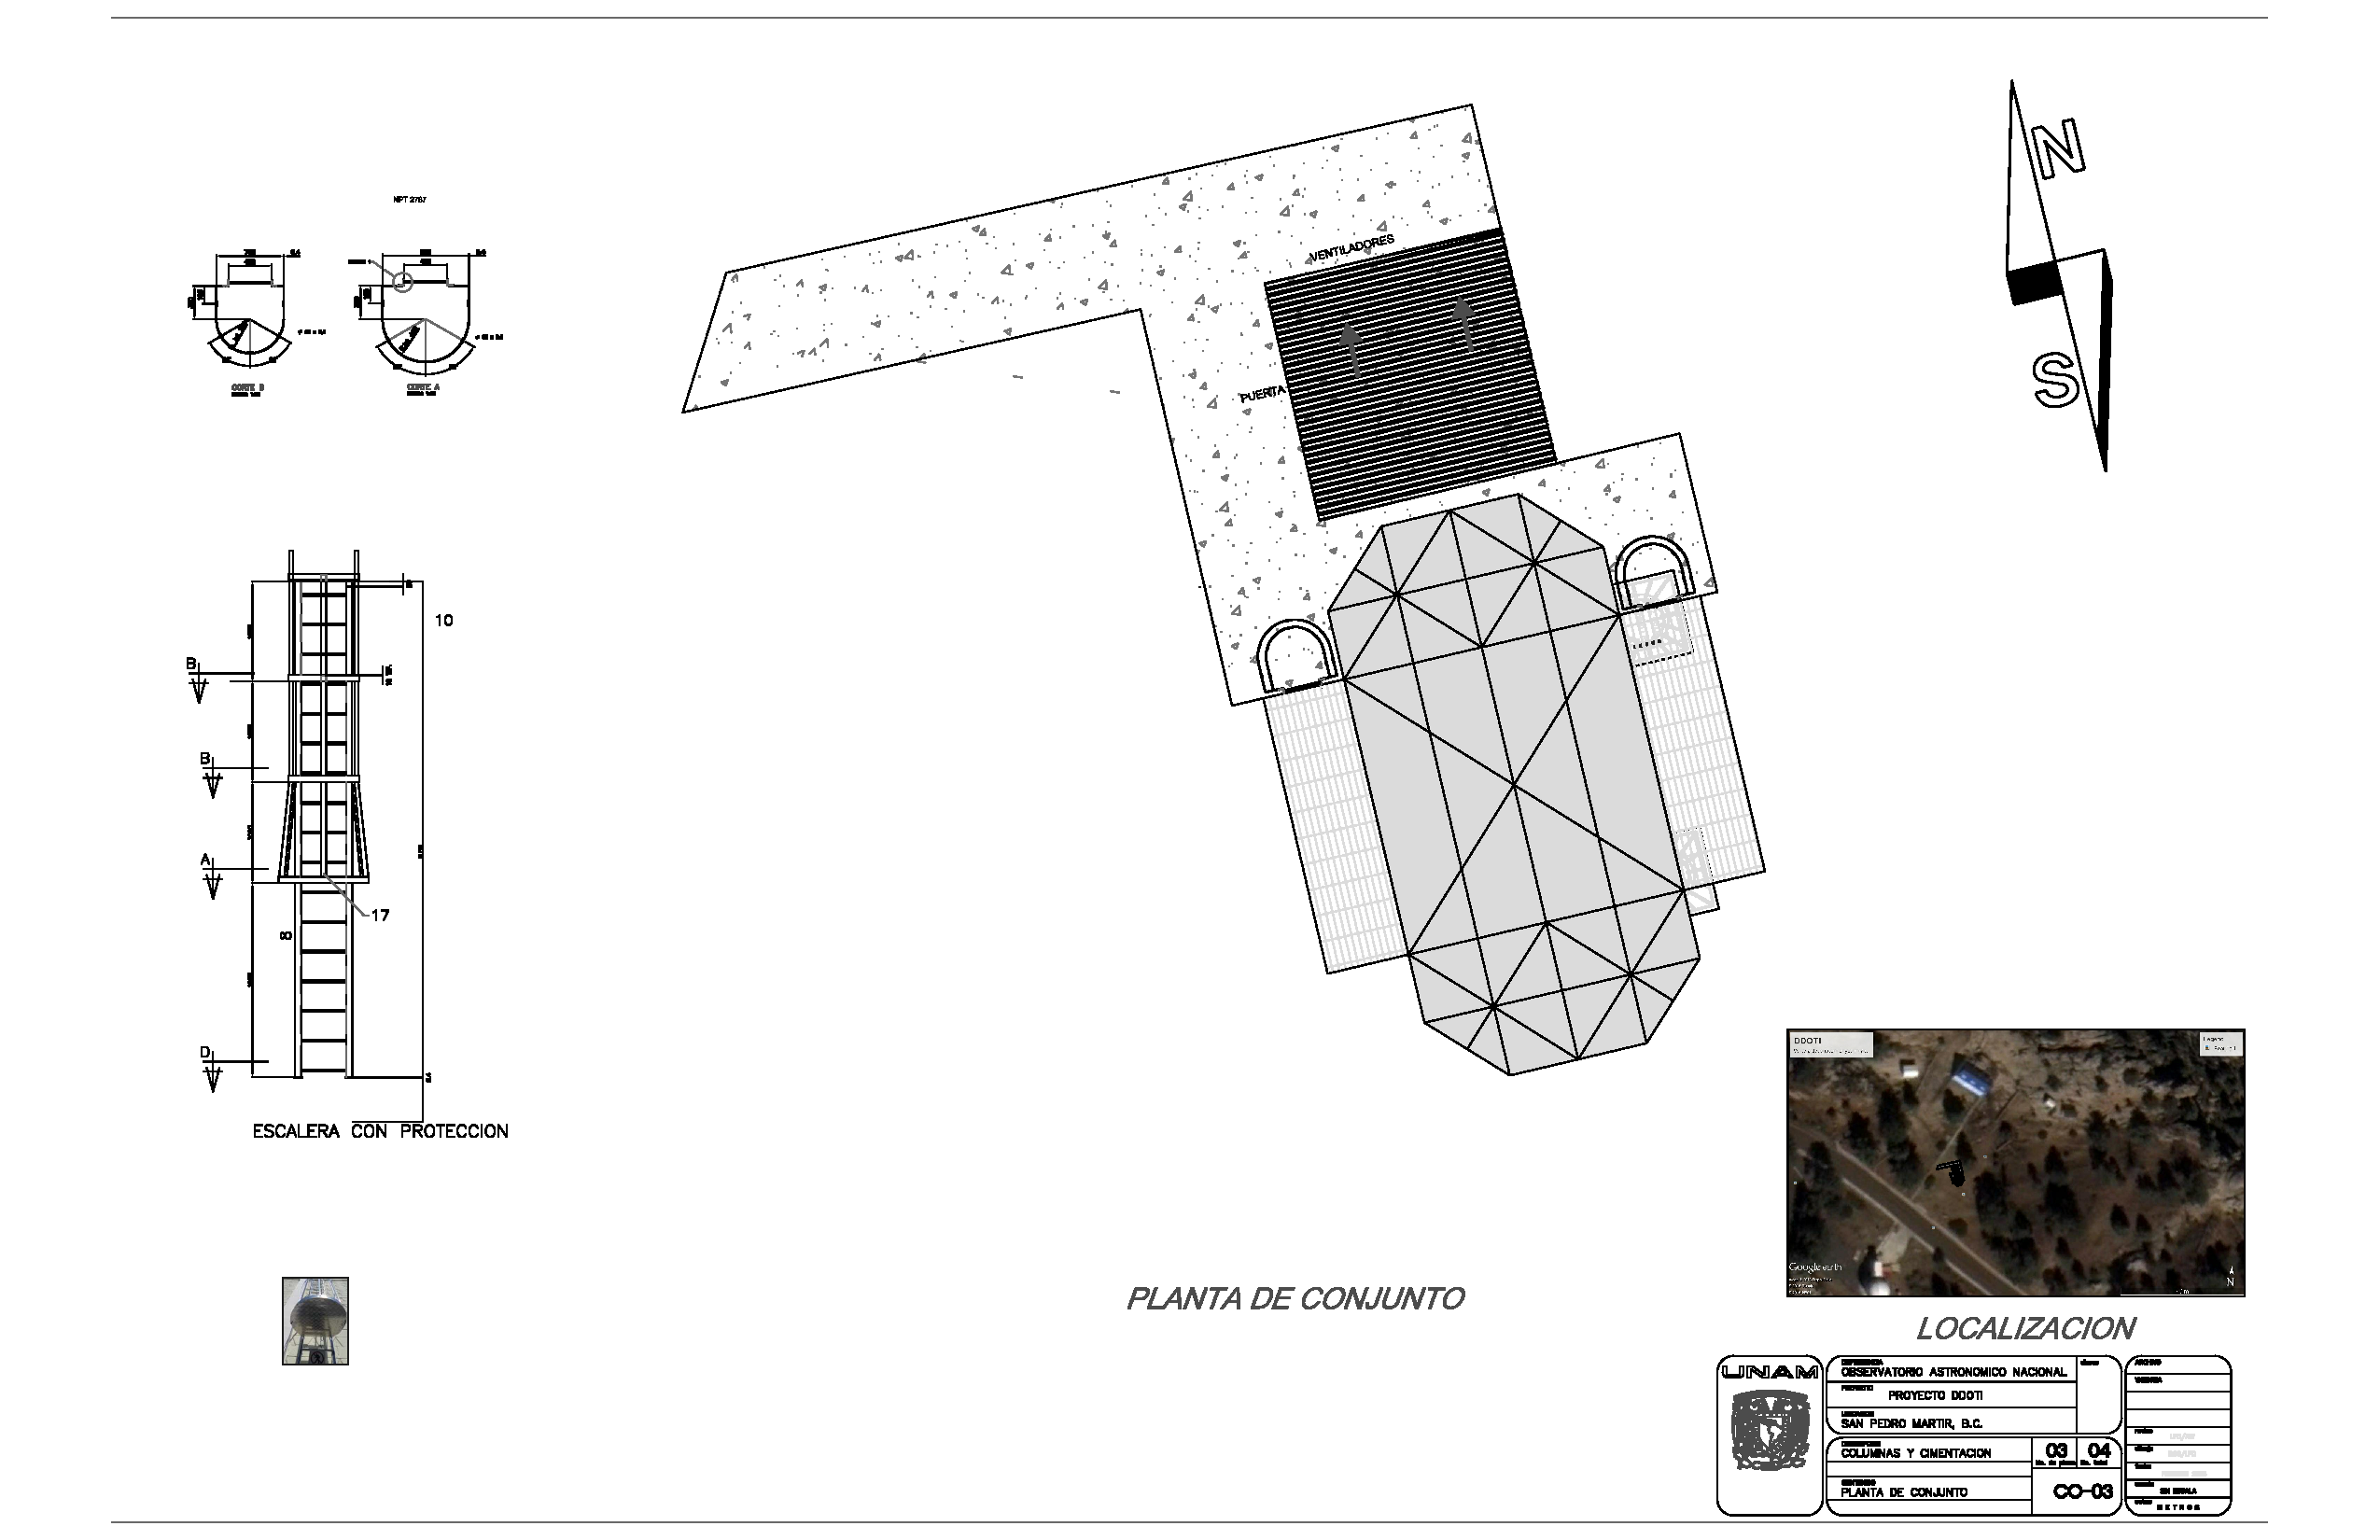
\includegraphics[height=0.8\linewidth,angle=90]{figures/buildings-ddoti-drawing-2016-2.pdf}
\end{center}
\caption{{\projectname} original 2016 design drawing (2 of 3). Note that the actual installation is rotated approximately 22 degrees east of the orientation shown here.}
\label{figure:buildings-drawing-2016-2}
\end{figure*}

\begin{figure*}
\begin{center}
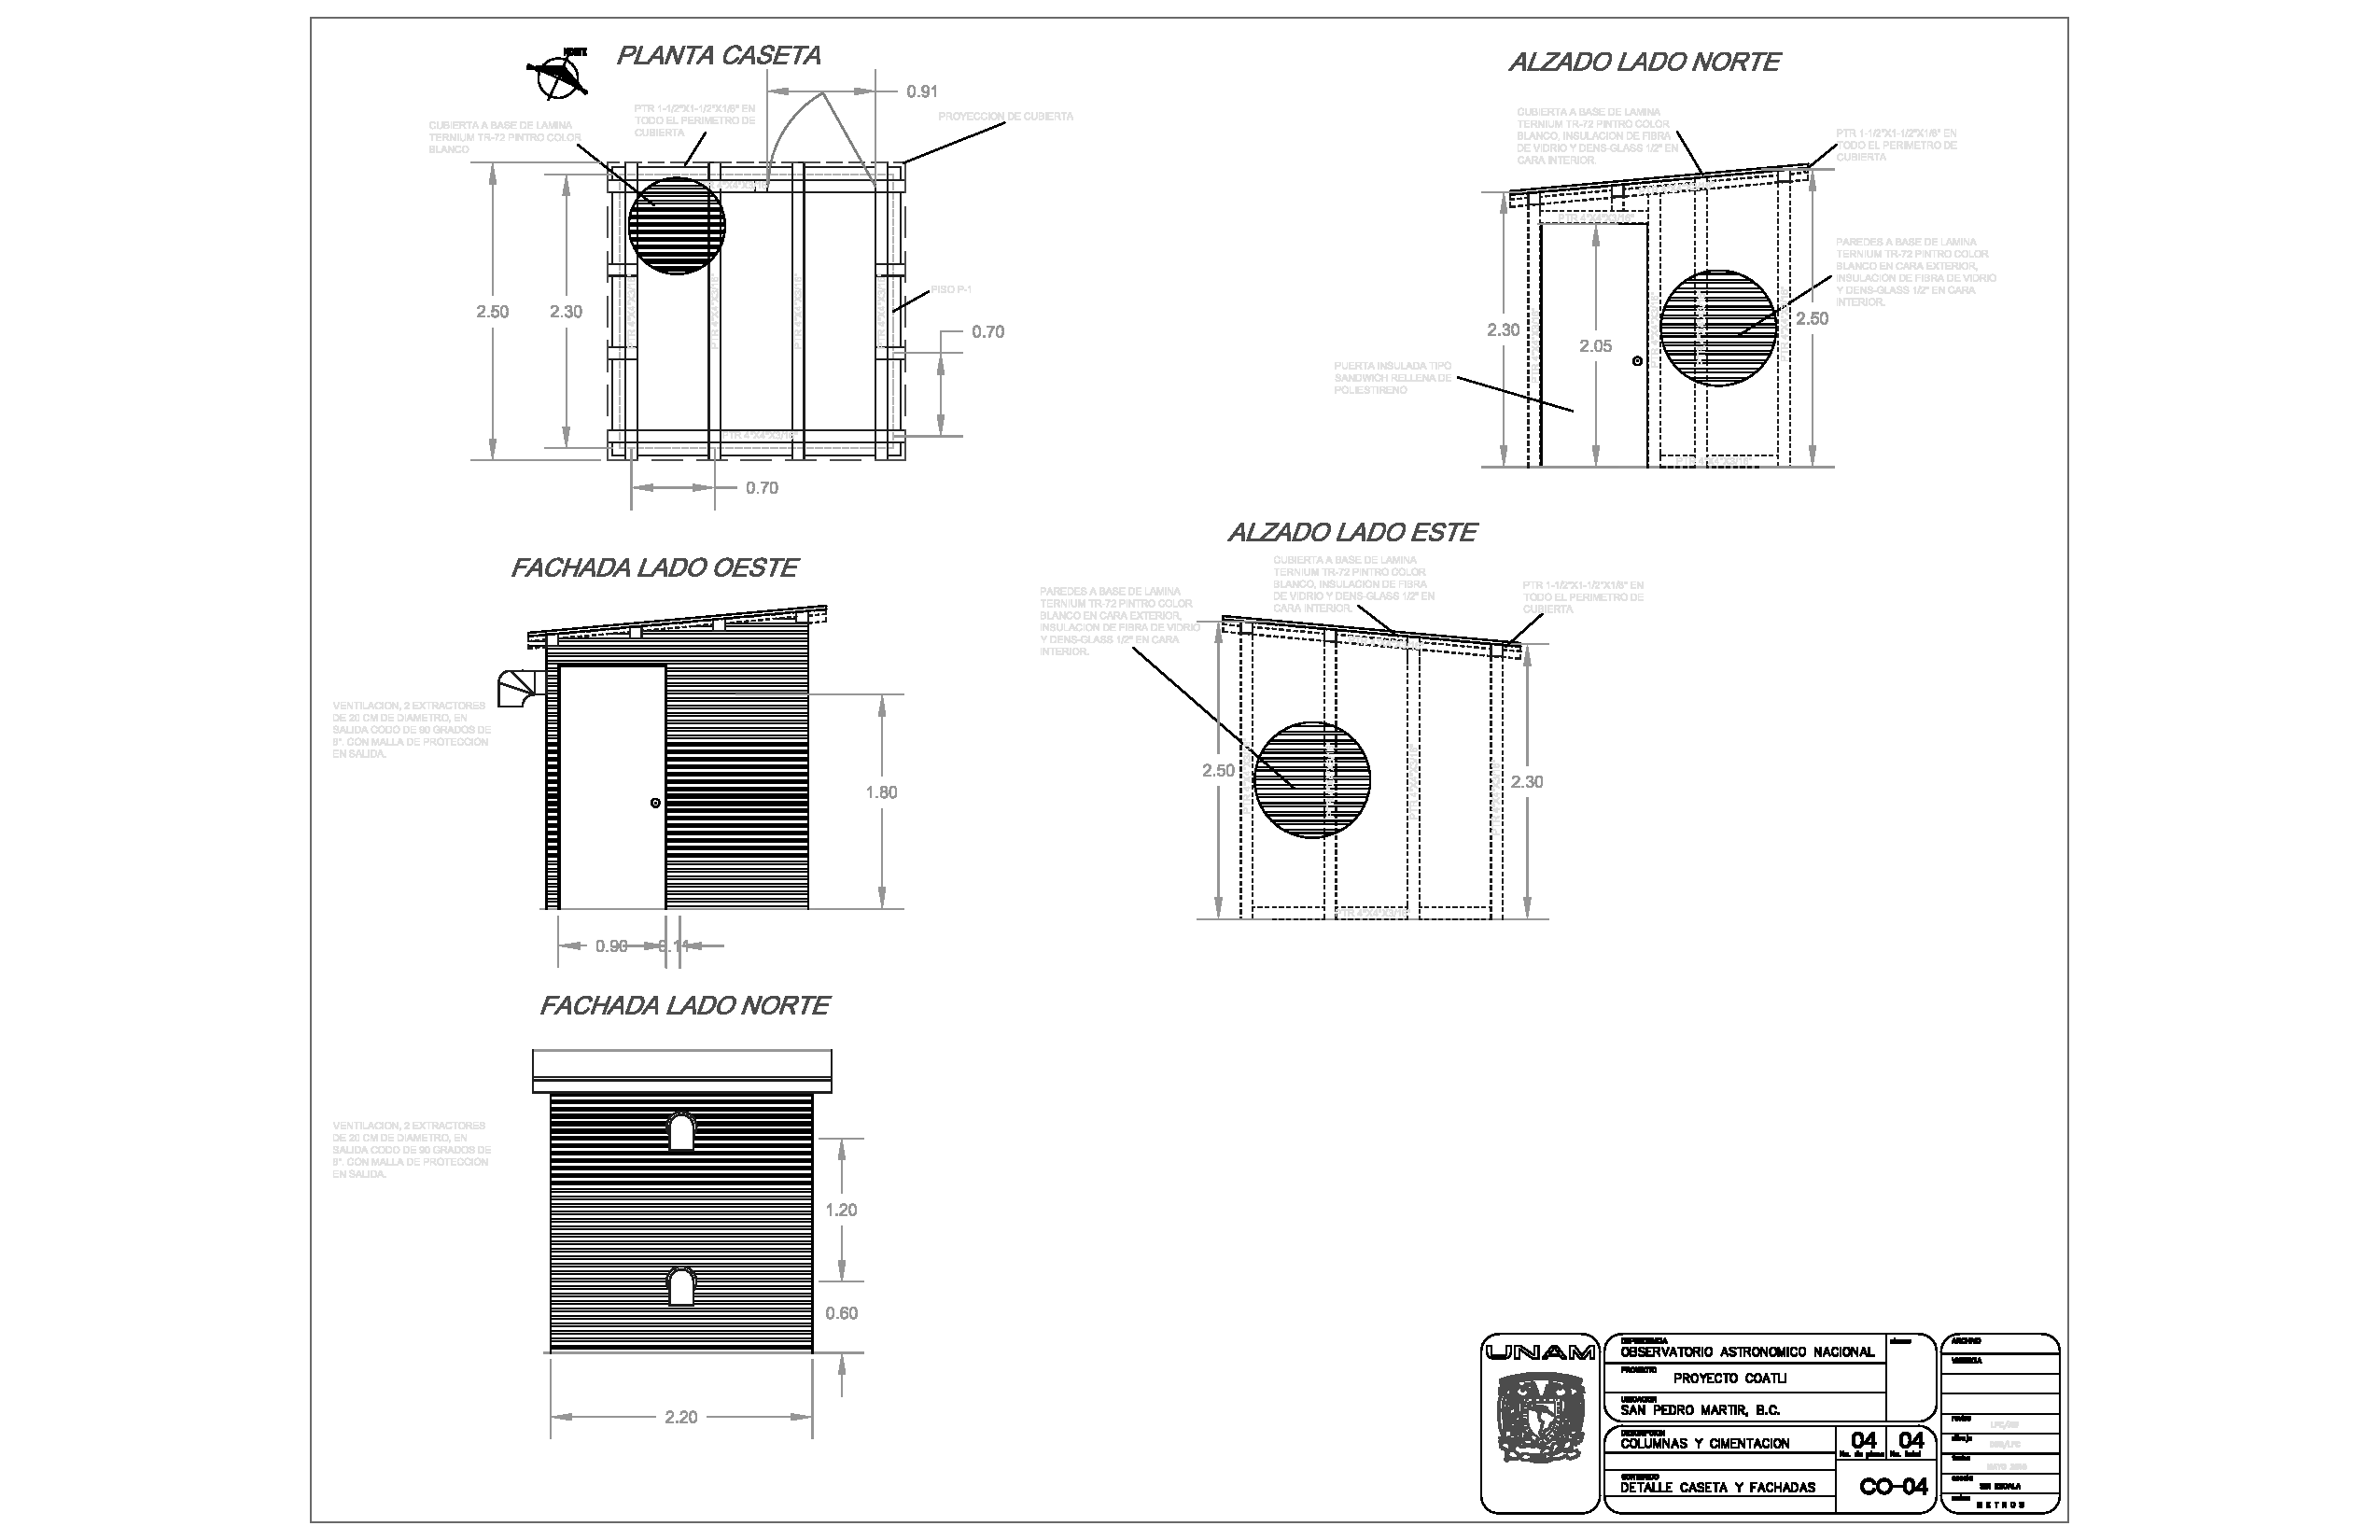
\includegraphics[height=0.95\linewidth,angle=90]{figures/buildings-ddoti-drawing-2016-3.pdf}
\end{center}
\caption{{\projectname} original 2016 design drawing (3 of 3).}
\label{figure:buildings-drawing-2016-3}
\end{figure*}

\begin{figure*}
\begin{center}
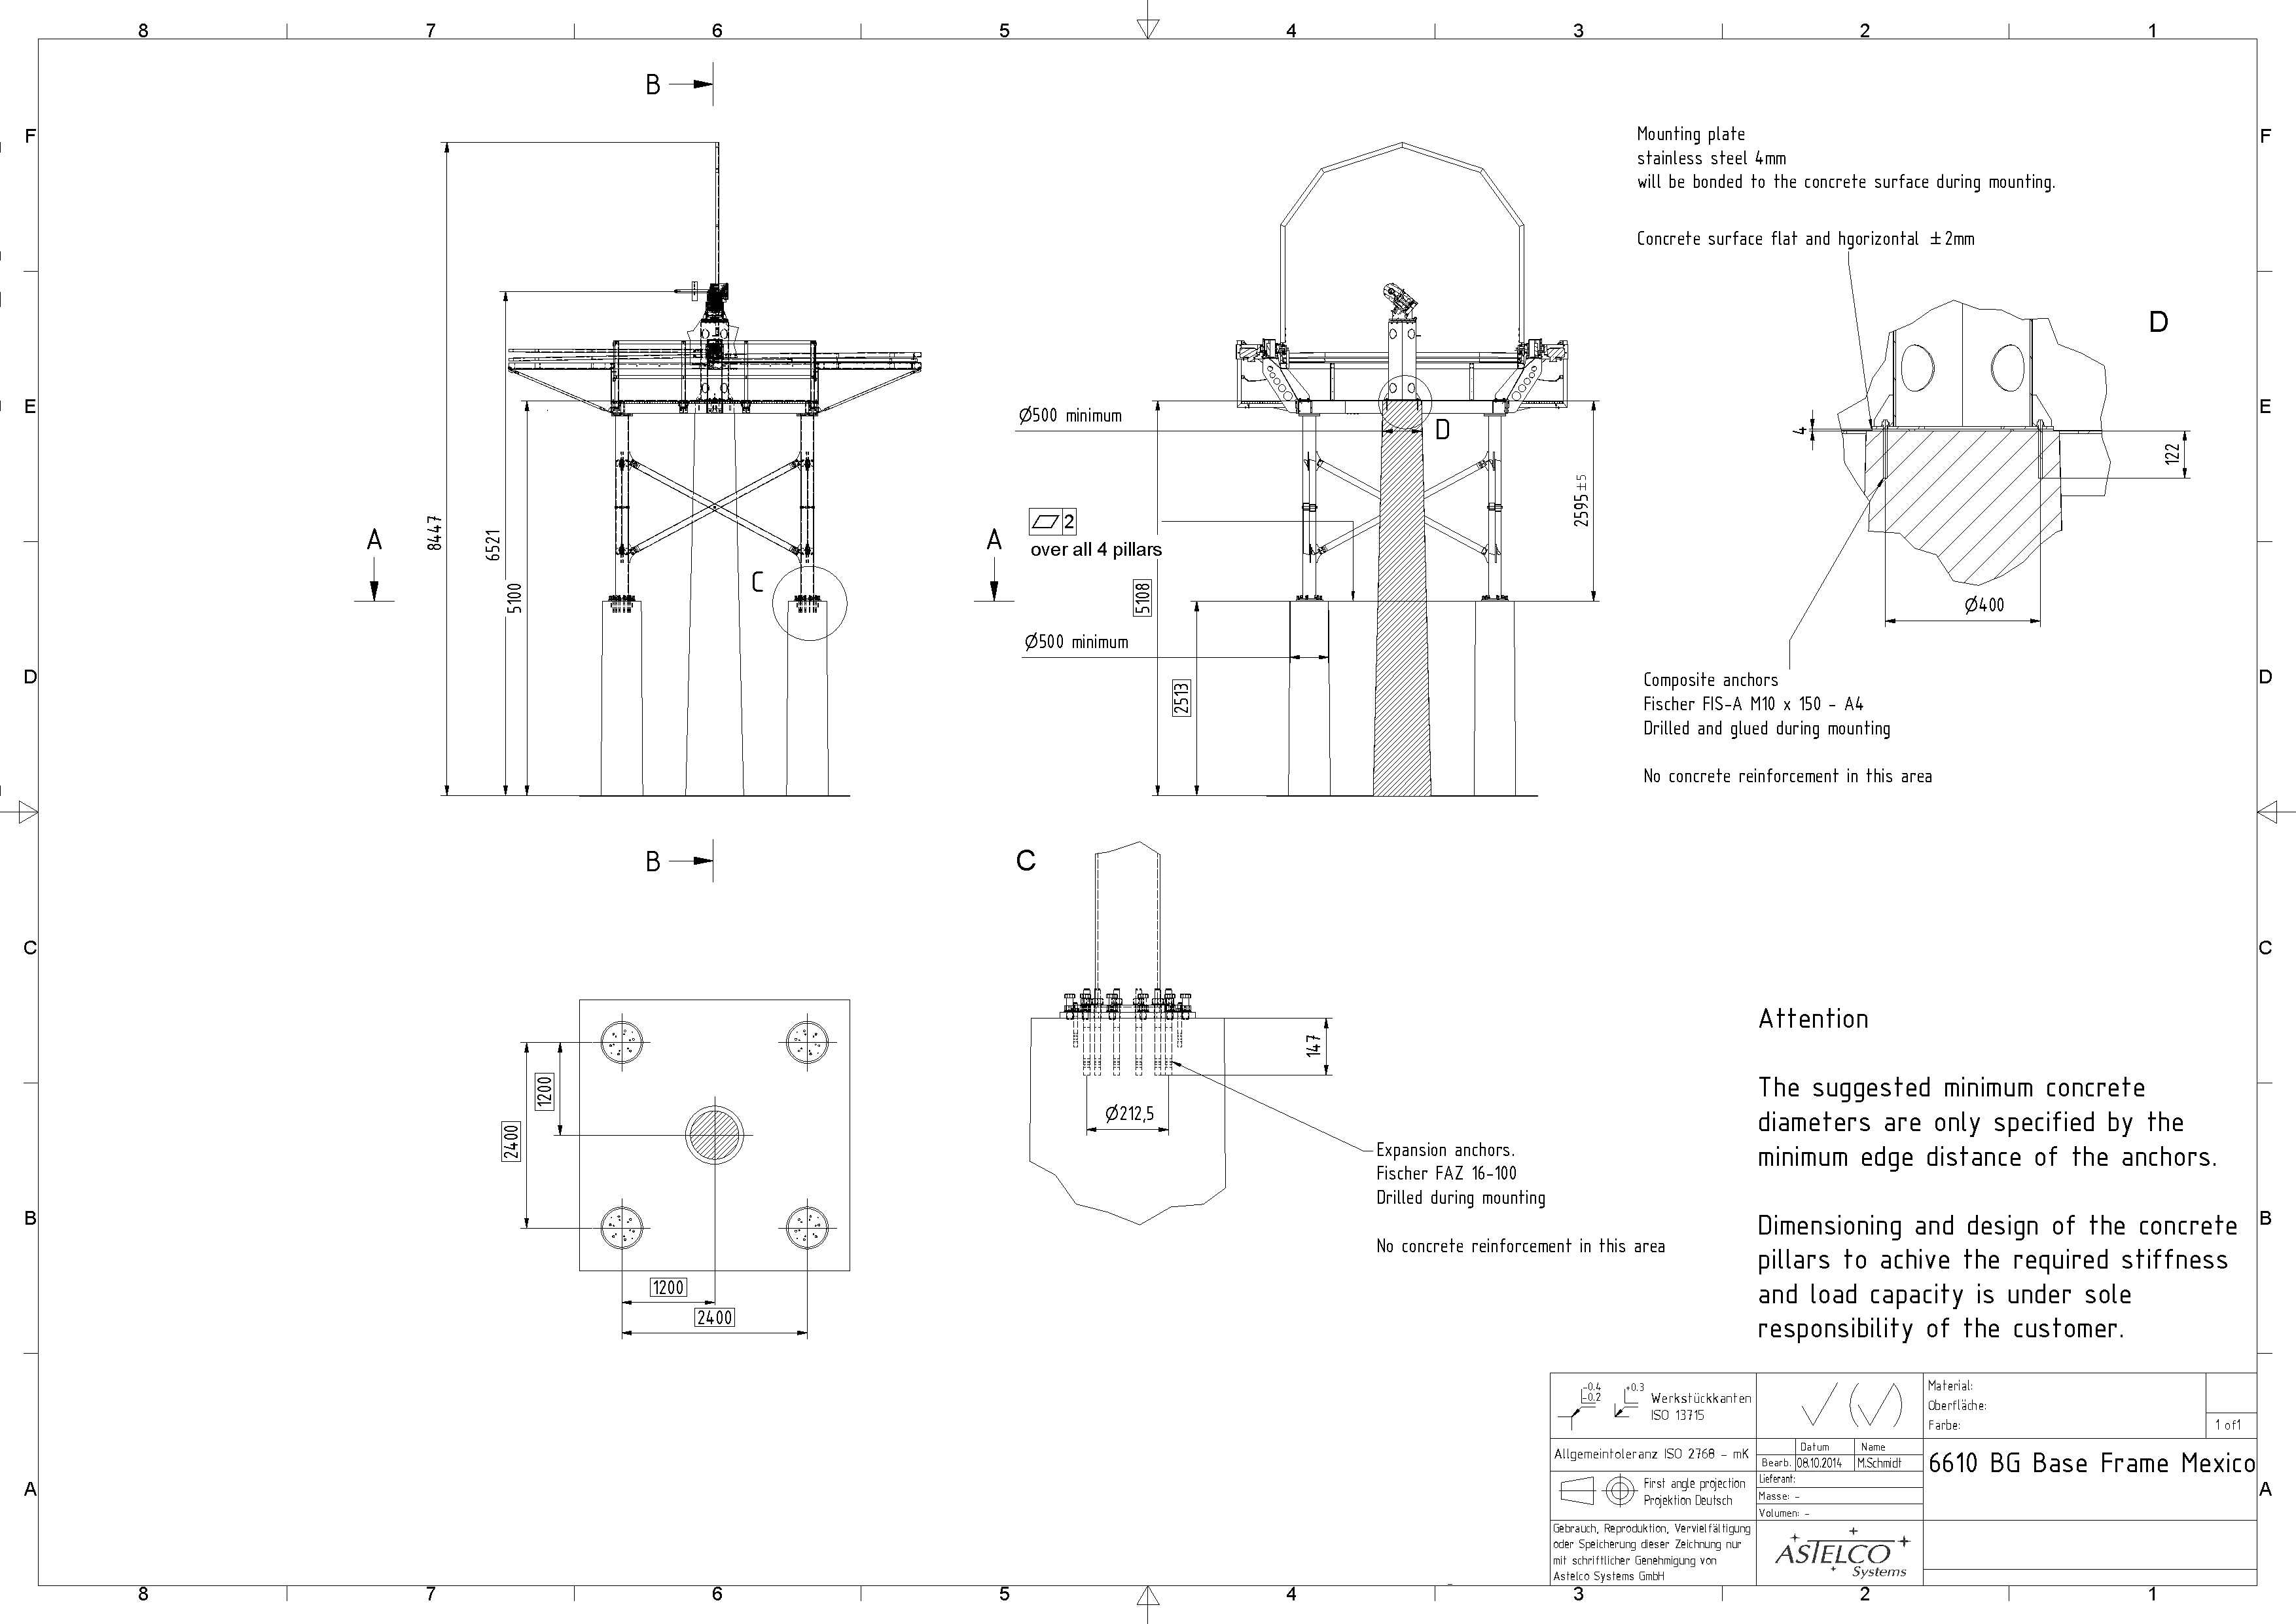
\includegraphics[height=0.95\linewidth,angle=90]{figures/buildings-ddoti-astelco-enclosure-drawing-6610}
\end{center}
\caption{{\projectname} ASTELCO platform and telescope pier (for COATLI).}
\label{figure:buildings-drawing-astelco}
\end{figure*}

\begin{figure*}
\begin{center}
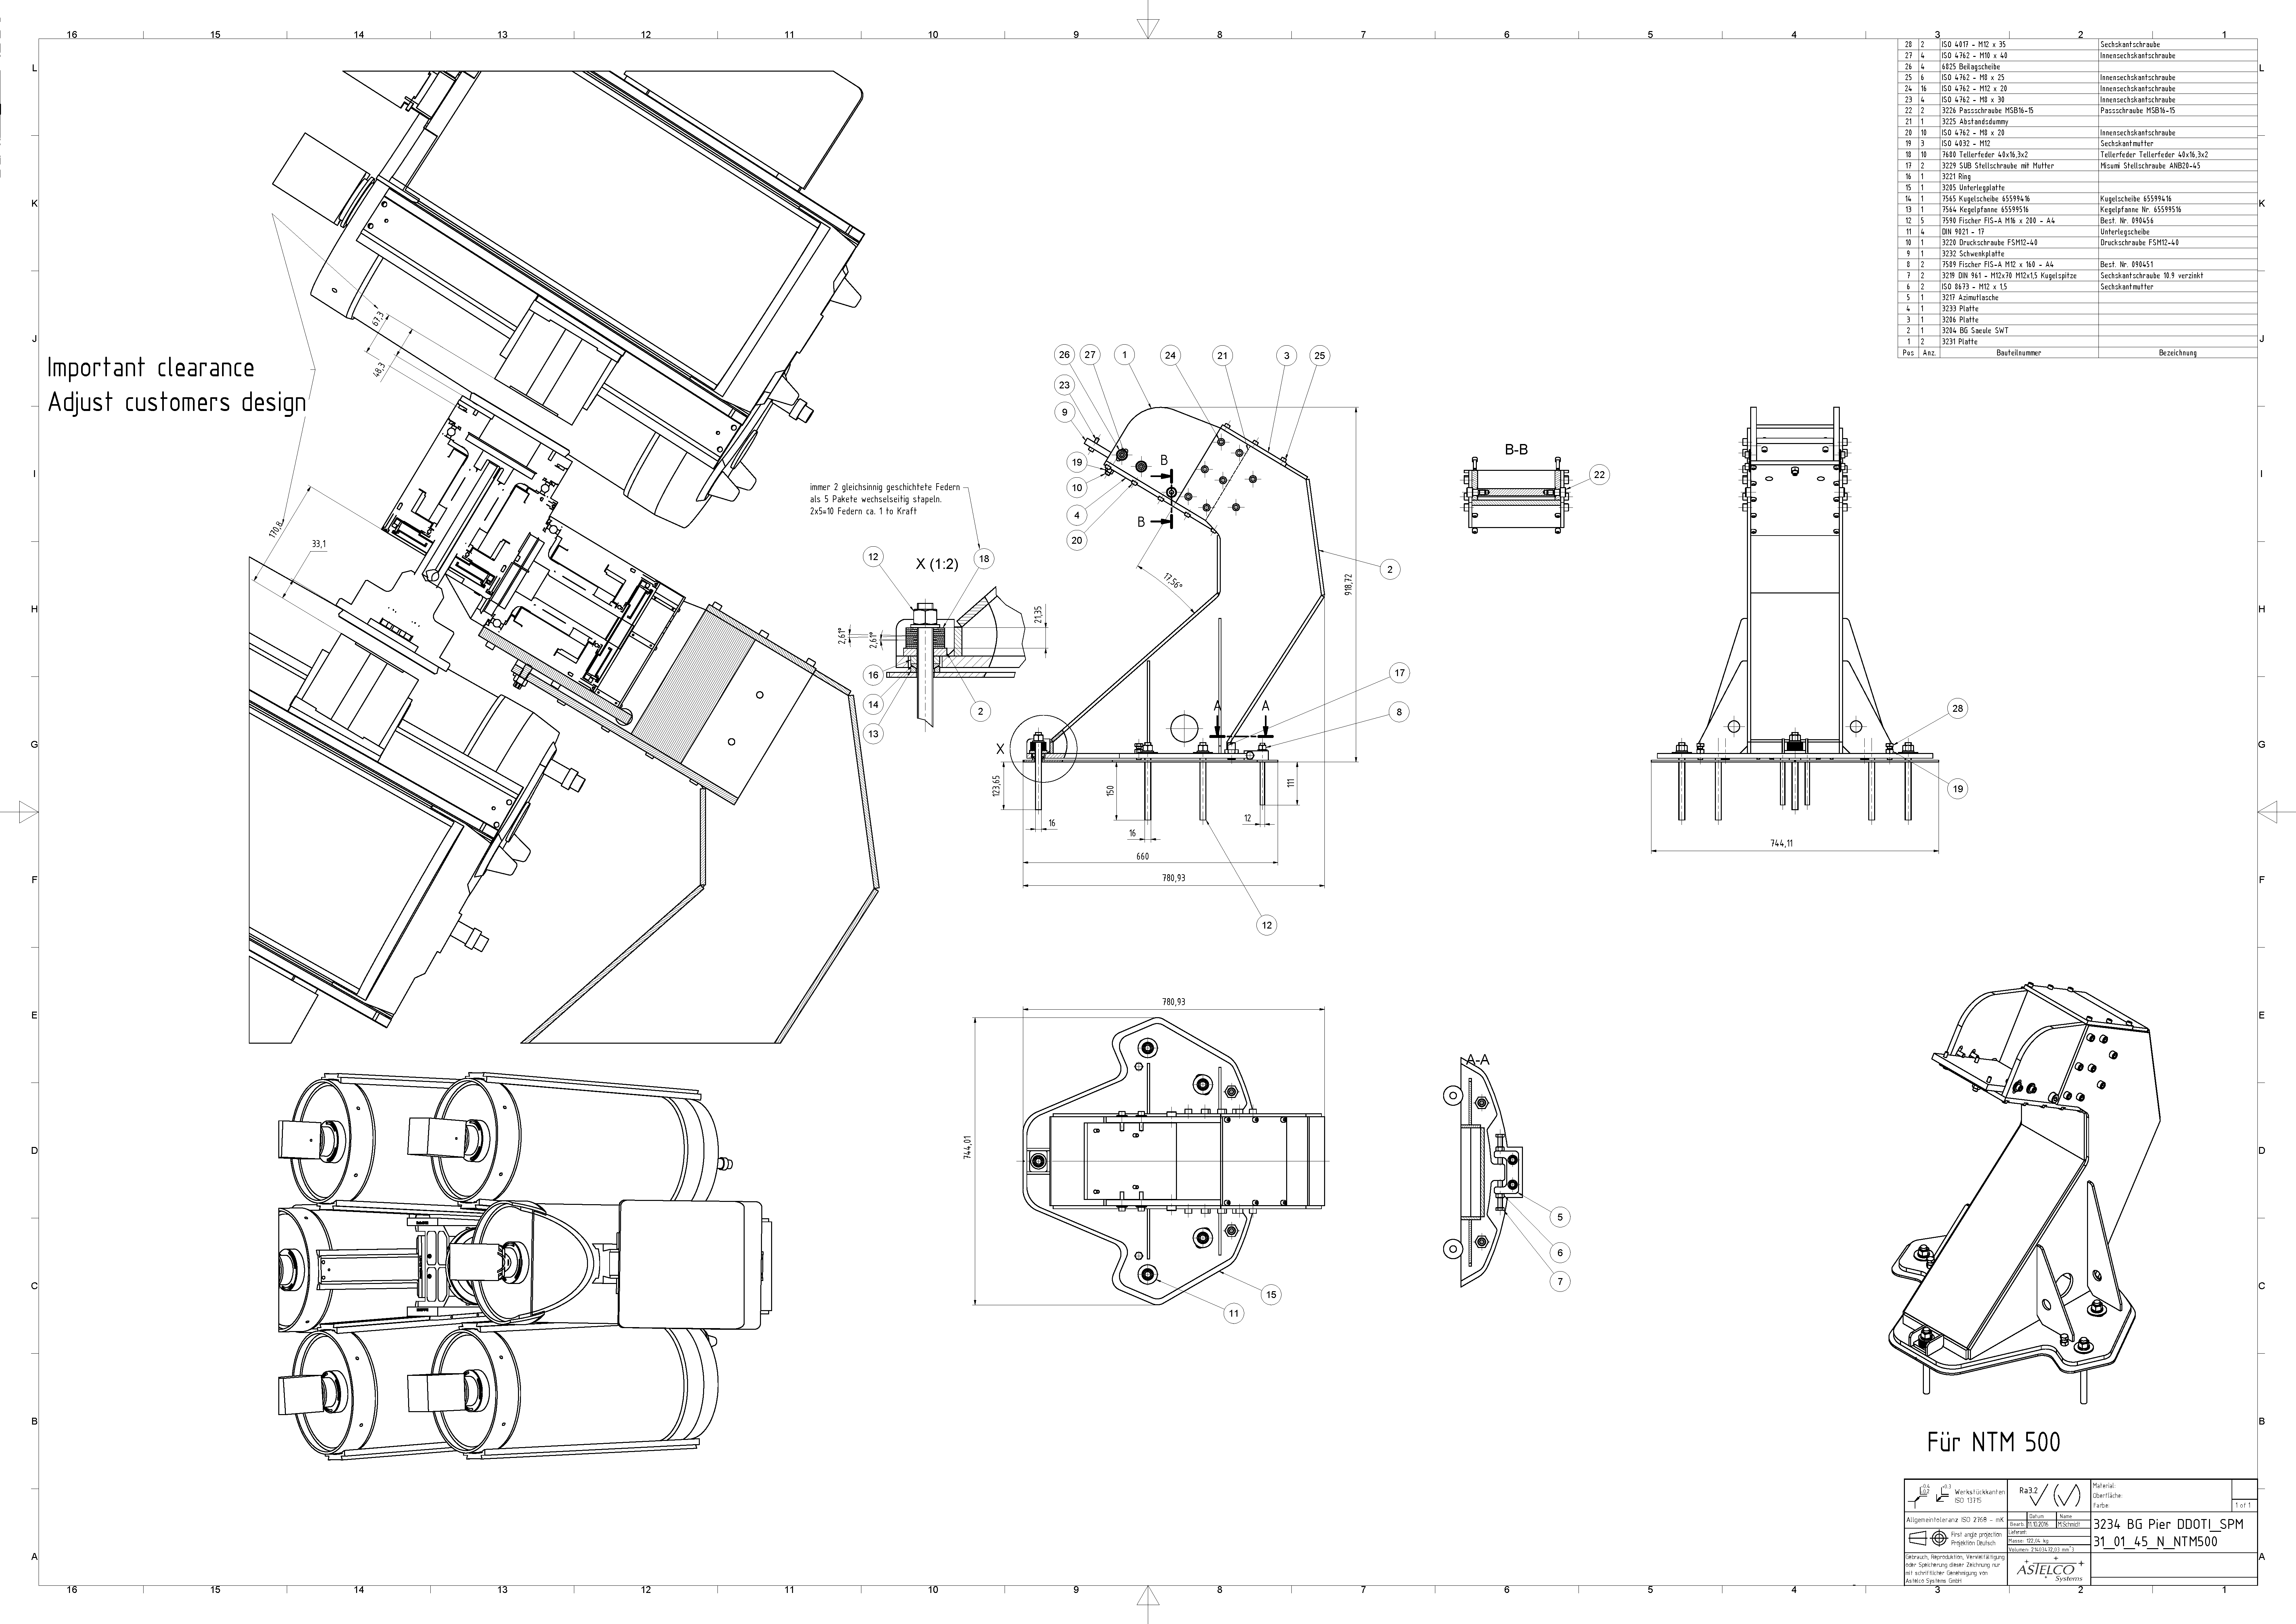
\includegraphics[height=0.95\linewidth,angle=90]{figures/buildings-ddoti-astelco-pier-drawing-3234}
\end{center}
\caption{{\projectname} ASTELCO pier.}
\label{figure:buildings-drawing-astelco-pier}
\end{figure*}

\fi

\section{Ground-Floor of the 84-cm Telescope Building}

We use the ground-floor of the 84-cm telescope building for storage of equipment and as a temporary work space.

{\projectname} tools and equipment are stored mainly in the equipment cabinet. They are to be used only for maintenance of COATLI and DDOTI and must be returned to the cabinet at the end of the maintenance procedure.

ASTELCO tools and equipment are stored in a locked metal box and are only to be used under the supervision of project or ASTELCO personnel.

\section{Shed}
\label{section:shed}
\label{section:shed-key}

The shed contains infrastructure and control electronics.

\begin{figure*}
\begin{center}
\begin{labeled}{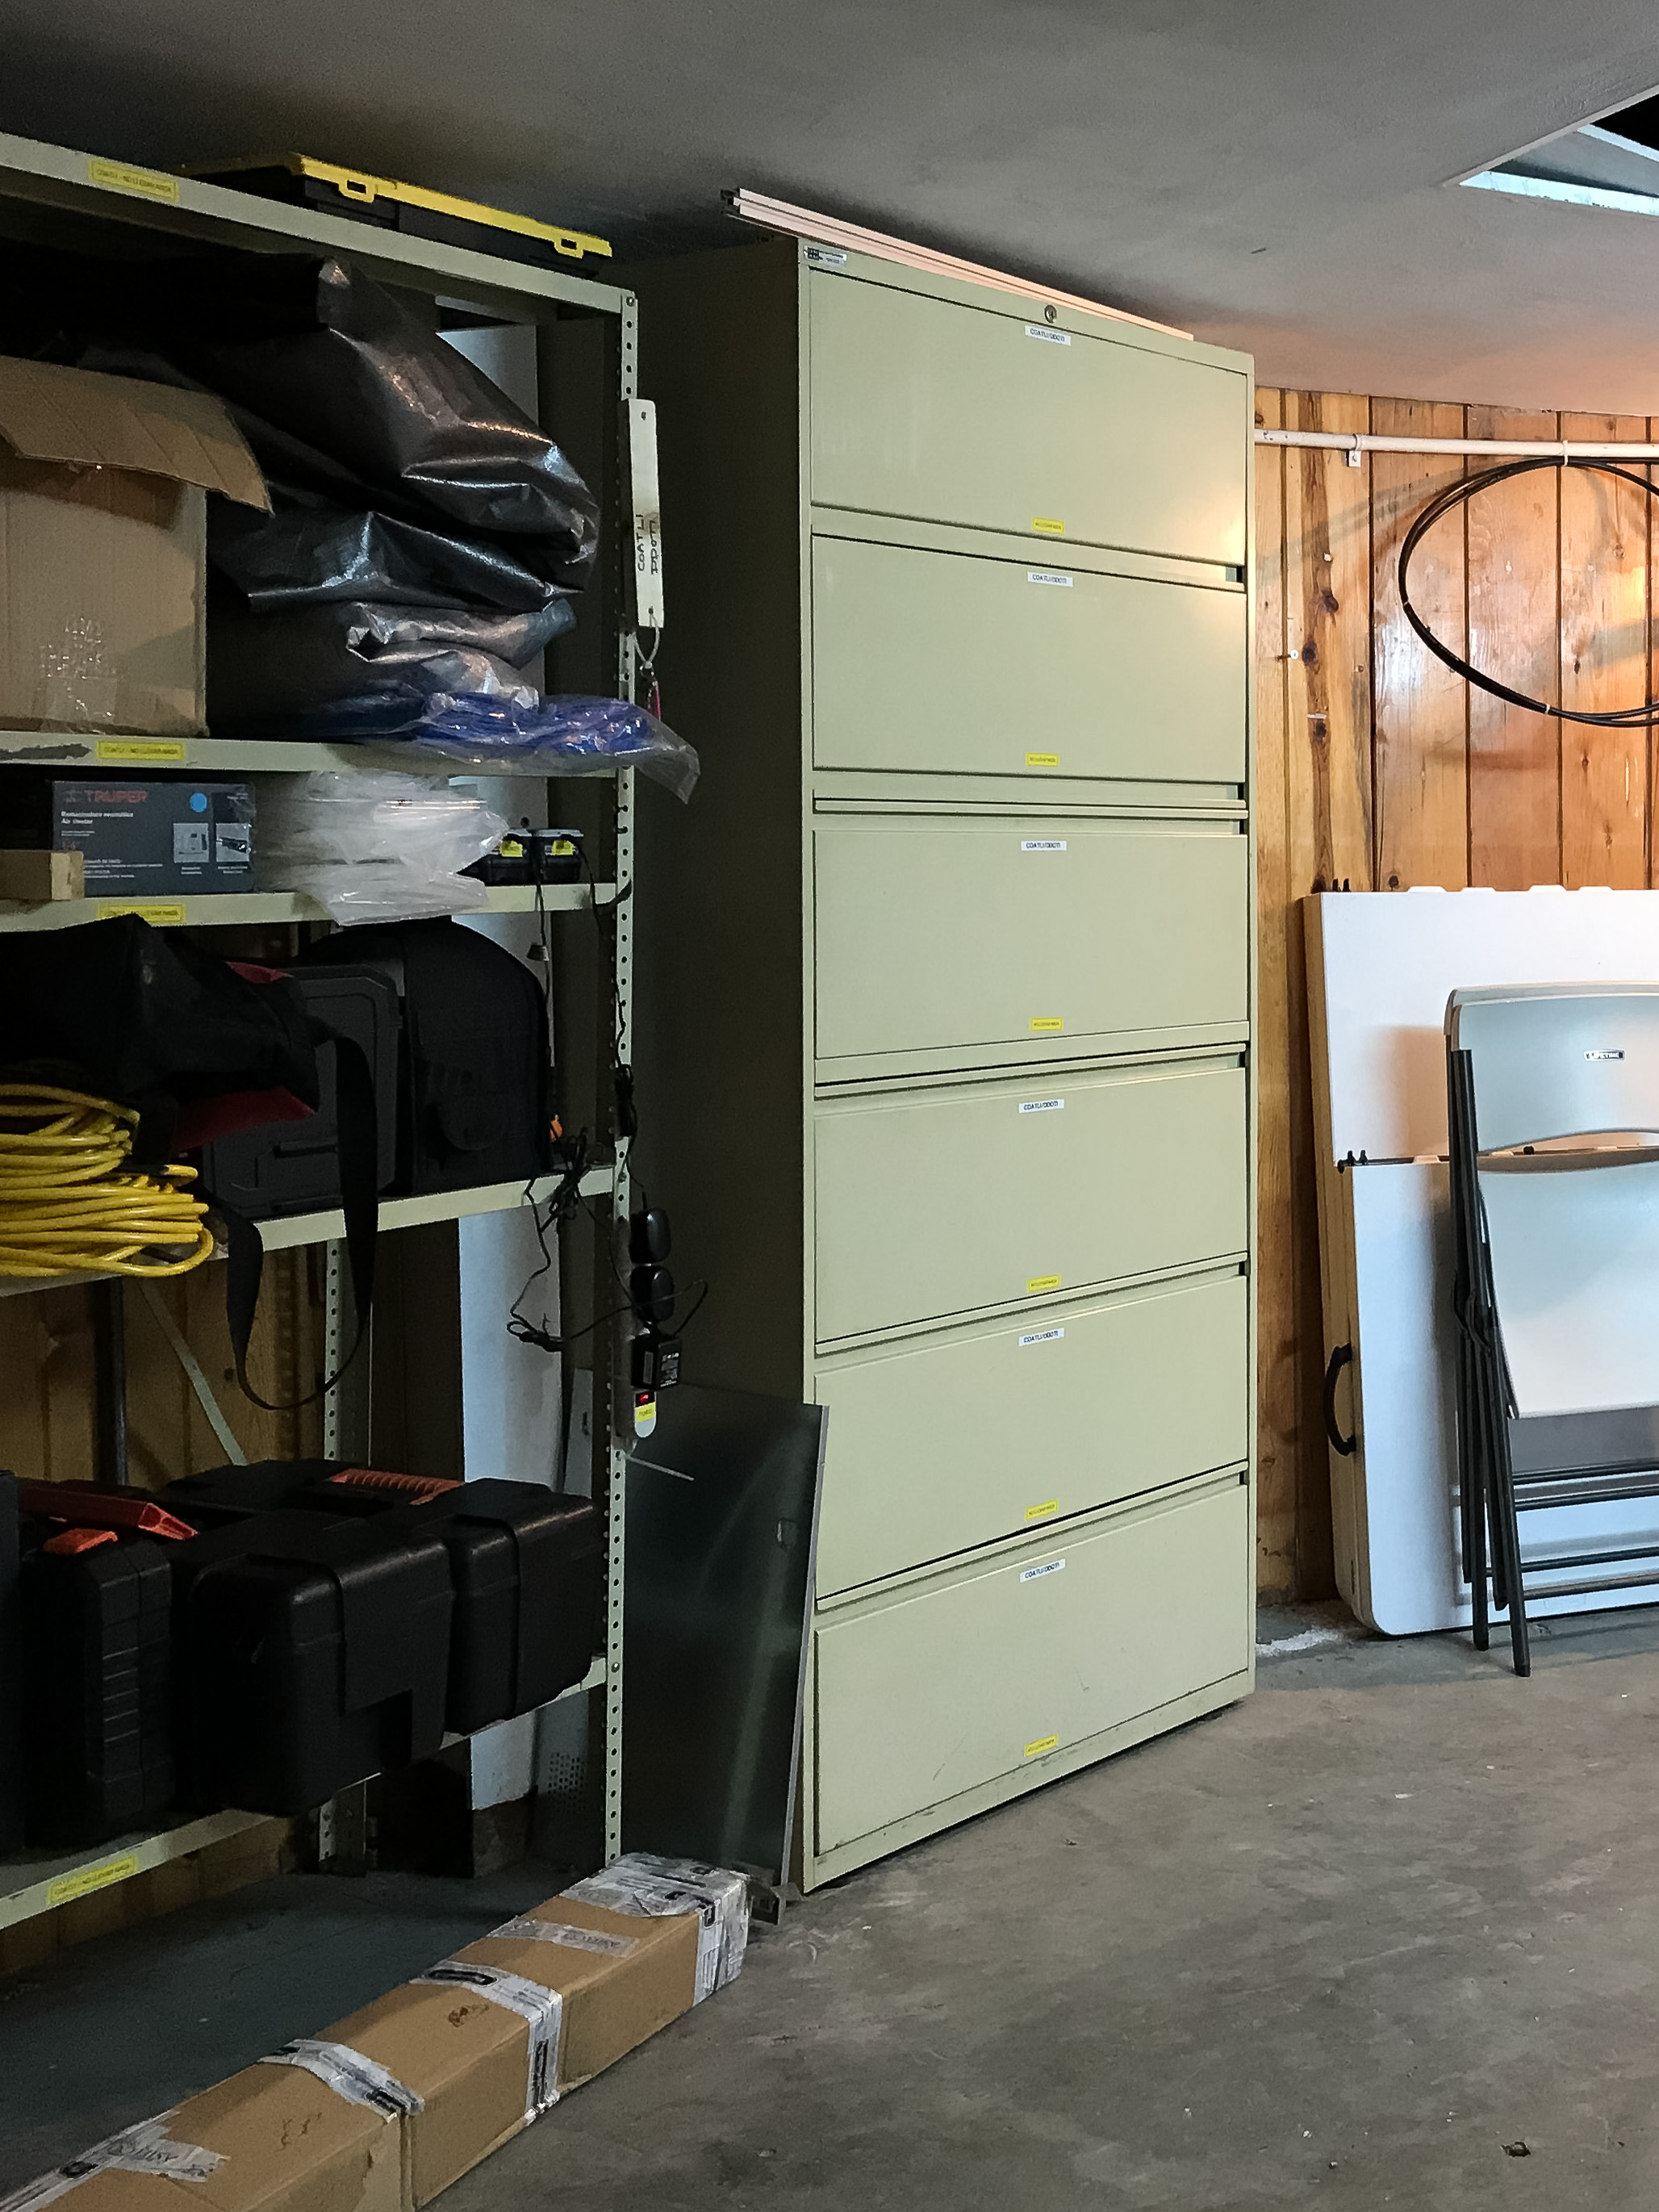
\includegraphics[width=0.8\linewidth]{figures/buildings-shed-key.jpg}}
\arrowandlabel{(-1,+3.5)}{(+0,+4)}{west}{Shed Key}
\end{labeled}
\end{center}
\caption{The shed key is hung on the shelves next to the cabinet in the ground floor of the 84-cm telescope building.}
\label{figure:buildings-shed-key}
\end{figure*}

The door to the shed should be left locked. 

The key should be hung on the shelves next to the cabinet in the ground-floor of the 84-cm telescope building (see Figure~\ref{figure:buildings-shed-key}).

The temperature in the shed it controlled by a heater and a pair of fans (one inlet and one exhaust). The fans are controlled by a Lux WIN100 thermostat and are set to turn on at 10 C. The internal thermostat of the heater is set to its minimum level.

%\section{Access Staircase and Walkways}

%\section{Tower, Platform, and Enclosure}

\section{Bibliography}

\begin{flushleft}
\begin{itemize}

\ifcoatli
\item “\href{bibliography/unam-coatli-building-drawing-2015-1.pdf}{Building 2015 Drawing 1 - Columns}”, UNAM.
\item “\href{bibliography/unam-coatli-building-drawing-2015-2.pdf}{Building 2015 Drawing 2 - Plan}”, UNAM.
\item “\href{bibliography/unam-coatli-building-drawing-2015-3.pdf}{Building 2015 Drawing 3 - Stairways}”, UNAM.
\item “\href{bibliography/unam-coatli-building-drawing-2015-4.pdf}{Building 2015 Drawing 4 - Shed}”, UNAM.
\item “\href{bibliography/unam-coatli-building-drawing-2015-5.pdf}{Building 2015 Drawing 5 - Location}”, UNAM.
\item “\href{bibliography/astelco-enclosure-drawing-0500}{ASTELCO Drawing 0500 -- Platform}”, ASTELCO.
\item “\href{bibliography/astelco-enclosure-drawing-5772}{ASTELCO Drawing 5572 -- Tower Mounting Plate}”, ASTELCO.
\item “\href{bibliography/astelco-enclosure-drawing-5772}{ASTELCO Drawing 5798 -- Tower}”, ASTELCO.
\item “\href{bibliography/astelco-enclosure-drawing-5772}{ASTELCO Drawing 6610 --  Tower, Platform, and Enclosure}”, ASTELCO.
\item “\href{bibliography/astelco-enclosure-drawing-5772}{ASTELCO Drawing 6658 -- Tower, Platform, and Enclosuure}”, ASTELCO.
\item “\href{bibliography/astelco-enclosure-drawing-5772}{ASTELCO Drawing 6662 -- Interface}”, ASTELCO.
\item “\href{bibliography/unam-coatli-building-drawing-2018-1.pdf}{Building 2018 Drawing 1 - Column}”, UNAM.
\item “\href{bibliography/unam-coatli-building-drawing-2018-2.pdf}{Building 2018 Drawing 2 - Floor Support Beams}”, UNAM.
\item “\href{bibliography/unam-coatli-building-drawing-2018-3.pdf}{Building 2018 Drawing 3 - Floor Support Beams}”, UNAM.
\fi

\ifddoti
\item “\href{bibliography/unam-ddoti-building-drawing-2016-1.pdf}{Building 2016 Drawing 1 - Columns}”, UNAM.
\item “\href{bibliography/unam-ddoti-building-drawing-2016-2.pdf}{Building 2016 Drawing 2 - Plan and Location}”, UNAM.
\item “\href{bibliography/unam-ddoti-building-drawing-2016-3.pdf}{Building 2015 Drawing 3 - Shed}”, UNAM.
\item “\href{bibliography/astelco-enclosure-drawing-0500}{ASTELCO Drawing 0500 -- Platform}”, ASTELCO.
\item “\href{bibliography/astelco-enclosure-drawing-5772}{ASTELCO Drawing 5572 -- Tower Mounting Plate}”, ASTELCO.
\item “\href{bibliography/astelco-enclosure-drawing-5772}{ASTELCO Drawing 6610 --  Tower, Platform, and Enclosure}”, ASTELCO.
\item “\href{bibliography/astelco-enclosure-drawing-5772}{ASTELCO Drawing 6658 -- Tower, Platform, and Enclosuure}”, ASTELCO.
\item “\href{bibliography/astelco-enclosure-drawing-5772}{ASTELCO Drawing 6662 -- Interface}”, ASTELCO.
\item “\href{bibliography/astelco-ddoti-pier-drawing-3205}{ASTELCO Drawing 3205 -- Pier Mounting Plate}”, ASTELCO.
\item “\href{bibliography/astelco-ddoti-pier-drawing-3205}{ASTELCO Drawing 3234 -- Pier}”, ASTELCO.
\fi

\item “\href{bibliography/lux-win100-manual}{Lux WIN100 Manual}”, Lux.

\end{itemize}
\end{flushleft}

\chapter{Electrical Power}
\label{chapter:electrical-power}

This chapter describes the electrical power system in the {\projectname} installation. The electrical grounding system is described in Chapter~\ref{chapter:electrical-grounding}.

Figure~\ref{figure:schematic-electrical-power}
shows a schematic of the electrical power system. The sections below describe each part in detail.

TODO: Don’t know which DDOTI circuits are L1-N, L2-N, or L3-N.

\begin{figure*}[p]
\begin{center} 
\resizebox{\columnwidth}{!}{
\begin{tikzpicture}
[
 thick,
 >={latex},
 box/.style={
  inner sep=1mm,
  draw=black,
  rectangle,
  minimum width=2cm,
  minimum height=0.6cm,
  align=center
 },
 circuit/.style={
  draw=black,
  rectangle,
  fill=white
 }
]

\ifcoatli
\node at (-6,-3) [box,minimum width=12cm,right] (oan) {OAN Grid};
\node at (-6,-1) [box,minimum width=12cm,right] (transformer) {Isolation Transformer};
\node at (-6,0) [box,minimum width=12cm,right] (main-breaker-box) {Main Breaker Box};
\fi
\ifddoti
\node at (-6,-2) [box,minimum width=12cm,right] (oan) {OAN Grid};
\node at (-6,-1) [box,minimum width=12cm,right] (transformer) {Isolation Transformer};
\node at (-6,1) [box,minimum width=12cm,right] (main-breaker-box) {Main Breaker Box};
\fi
\node at (-6,2) [box,minimum width=12cm,right] (circuit-box) {Circuit Box};
\draw[->] (oan) -- (transformer);
\draw[->] (transformer) -- (main-breaker-box);
\draw[->] (main-breaker-box) -- (circuit-box);

\node at (-5,+4) [box] (socket-a) {Socket A};
\node at (+3.5,+5) [box] (lights) {Lights};
\node at (+1,+9) [box] (mount) {Mount};
\node at (-0.75,+4) [box] (socket-b) {Socket B};
\node at (+2,+4) [box] (sockets-d) {Sockets D};
\node at (+5,+4) [box] (socket-f) {Socket F};
\node at (-0.75,+5) [box] (ups-127) {127 V UPS};
\node at (-2,+6) [box] (ibb-127) {127 V iBB};
\node at (-5,+5) [box] (ups-220) {220 V UPS};
\node at (-5,+6) [box] (ibb-220) {220 V iBB};
\node at (-6,+7.5) [box,left] (enclosure) {Enclosure};
\ifcoatli
\node at (-6,+8.5) [box,left] (secondary) {Secondary};
\fi
\node at (+0,+7) [box,right] (rack-power-strip) {Rack Power Strip};
\node at (+0,+8) [box,right] (other-shed-electronics) {Other Shed Electronics};
\node at (+2,+6) [box] (fans-and-heater) {Fans and Heater};
\node at (+1,+11) [box,right] (platform-box) {Platform Box};
\ifcoatli
\node at (+1,+13) [box,right] (instrument-box) {Instrument Box};
\fi
\ifddoti
\node at (-1,+13) [box,right] (instrument0-box) {Instrument0 Box};
\node at (+3,+13) [box,right] (instrument1-box) {Instrument1 Box};
\fi
\node at (-3.0,+11) [box] (power-box) {Power Box};

\draw[->] 
 ($(circuit-box.north) + (-5.0,0)$) 
 -- node [circuit] {\scriptsize A} +(0,1)
 -- (socket-a);
\draw[->] 
 ($(circuit-box.north) + (-3.5,0)$) 
 -- node [circuit] {\scriptsize C} +(0,1)
 -- ($(power-box.south) + (-0.5,0)$);
\draw[->] 
 ($(circuit-box.north) + (-0.75,0)$) 
 -- node [circuit] {\scriptsize B} +(0,1)
 -- (socket-b.south);
\draw[->]
 ($(circuit-box.north) + (2,0)$) 
 -- node [circuit] {\scriptsize D} +(0,1)
 -- (sockets-d.south);
\draw[->] 
 ($(circuit-box.north) + (3.5,0)$) 
 -- node [circuit] {\scriptsize E} +(0,1)
 -- (lights.south);
\draw[->] 
 ($(circuit-box.north) + (5.0,0)$) 
 -- node [circuit] {\scriptsize F} +(0,1)
 -- (socket-f.south);

\draw[->] (socket-a) -- (ups-220);
\draw[->] (ups-220) -- (ibb-220);
\draw[->] 
 ($(ibb-220.north) + (-0.3,0)$)
 -- node [circuit] {\scriptsize A} +(0,1) 
 |- (enclosure.east);
\ifcoatli
\draw[->] 
 ($(ibb-220.north) + (+0.3,0)$)
 -- node [circuit] {\scriptsize A} +(0,1) 
 |- (secondary.east);
\fi

\draw[->] (socket-b) -- (ups-127);
\draw[->] ($(ups-127.north) + (-0.75,0)$) -- ($(ibb-127.south) + (+0.50,0)$);
\draw[->] ($(ups-127.north) + (-0.50,0)$) -- ($(ibb-127.south) + (+0.75,0)$);
\draw[->] ($(ups-127.north) + (+0.50,0)$) -- node [circuit] {\scriptsize B} +(0,1) |- (rack-power-strip.west);

\draw[->] 
 ($(ibb-127.north) + (-0.75,0)$)
 -- node [circuit] {\scriptsize B1} +(0,1)
 -- +(0,2)
 -| ($(power-box.south) + (+0.0,0)$);
\draw[->] 
 ($(ibb-127.north) + (-0.25,0)$)
 -- node [circuit] {\scriptsize B2} +(0,2)
 -- +(0,2.5)
 -| ($(power-box.south) + (+0.5,0)$);
\draw[->] 
 ($(ibb-127.north) + (+0.25,0)$) 
 -- node [circuit] {\scriptsize B} +(0,1)
 |- (mount.west);
\draw[->] 
 ($(ibb-127.north) + (+0.75,0)$) 
 -- node [circuit] {\scriptsize B} +(0,1)
 |- (other-shed-electronics.west);

\draw[->] 
 ($(power-box.east) + (0,-0.15)$)
 -- node [circuit] {\scriptsize B1} +(1,0)
 -- ($(platform-box.west) + (0,-0.15)$);
\draw[->] 
 ($(power-box.east) + (0,+0.15)$)
 -- node [circuit] {\scriptsize C} +(2.5,0)
 -- ($(platform-box.west) + (0,+0.15)$);

\ifcoatli
\draw[->] 
  (power-box.north) 
  -- node [circuit] {\scriptsize B2} +(0,0.7) 
  |- (instrument-box);
\fi
\ifddoti
\draw[->] 
  (power-box.north) 
  -- node [circuit] {\scriptsize B2} +(0,0.7) 
  |- (instrument0-box);
\draw[->] 
  (instrument0-box.east) 
  -- node [circuit] {\scriptsize B2} +(0.7,0) 
  |- (instrument1-box);
\fi

\draw[->] 
 (sockets-d.north) 
 -- node [circuit] {\scriptsize D} +(0,1)
 -- (fans-and-heater.south);

\draw[dashed] (-8,+10) -- (6.5,+10);
\draw[dashed] (-8,+12) -- (6.5,+12);
\draw[dashed] (-8,+14) -- (6.5,+14);
\node at (-8,+11) [right] {\normalsize Platform};
\node at (-8,+13) [right] {\normalsize Telescope};
\node at (-8,+6) [right] {\normalsize Shed};
\ifcoatli
\draw[dashed] (-8,-2) -- (6.5,-2);
\draw[dashed] (-8,+1) -- (6.5,+1);
\node at (-8,-0.5) [right] {\normalsize 84-cm};
\fi
\ifddoti
\draw[dashed] (-8,0) -- (6.5,0);
\fi

\end{tikzpicture}
}
\end{center}
\caption{Schematic of the Distribution of Electrical Power. The letters A to F refer to circuits.}
\label{figure:schematic-electrical-power}
\end{figure*}

\section{External Mains Supply}

The OAN electricity supply is 220~V 60~Hz three-phase.

\ifcoatli
The {\projectname} installation is connected to the OAN electricity supply via a spur to the circuit box in the 84-cm telescope building. This spur carries two phases (L1 and L2) and neutral (N). The phases are protected by an 80 A breaker. The circuit box and the breaker are shown in Figure~\ref{figure:main-breaker-box}.

\begin{figure}[t]
\begin{center}
\begin{labeled}{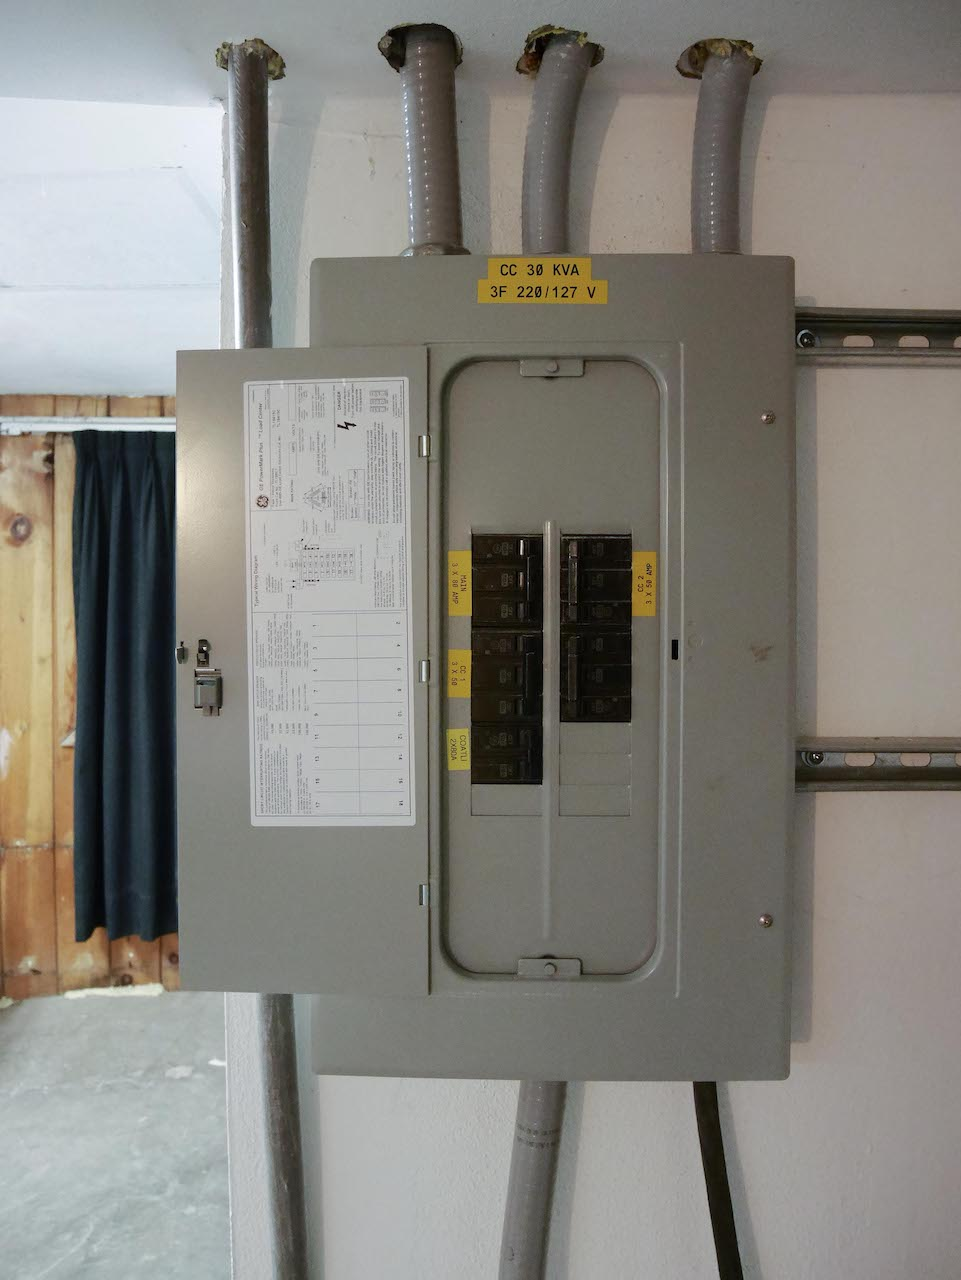
\includegraphics[height=0.7\linewidth]{figures/electrical-power-coatli-main-breaker-box.jpg}}
\arrowandlabel{(0.2,-1.0)}{(0,-5)}{north}{{\projectname} Main breaker}
\end{labeled}
\end{center}
\caption{The main breaker box in the 84-cm telescope building. The main breaker for the {\projectname} spur are at the lower left.}
\label{figure:main-breaker-box}
\end{figure}
\fi

\ifddoti
The {\projectname} installation is connected to the OAN electricity supply via an isolation transformer (on the north wall of the shed). This spur carries three phases (L1, L2, and L3) and neutral (N). The phases are protected by a 70~A breaker on a 30 kVA main breaker box inside the shed. The main breaker box is shown in Figure~\ref{figure:main-breaker-box}.

\begin{figure}[t]
\begin{center}
\begin{labeled}{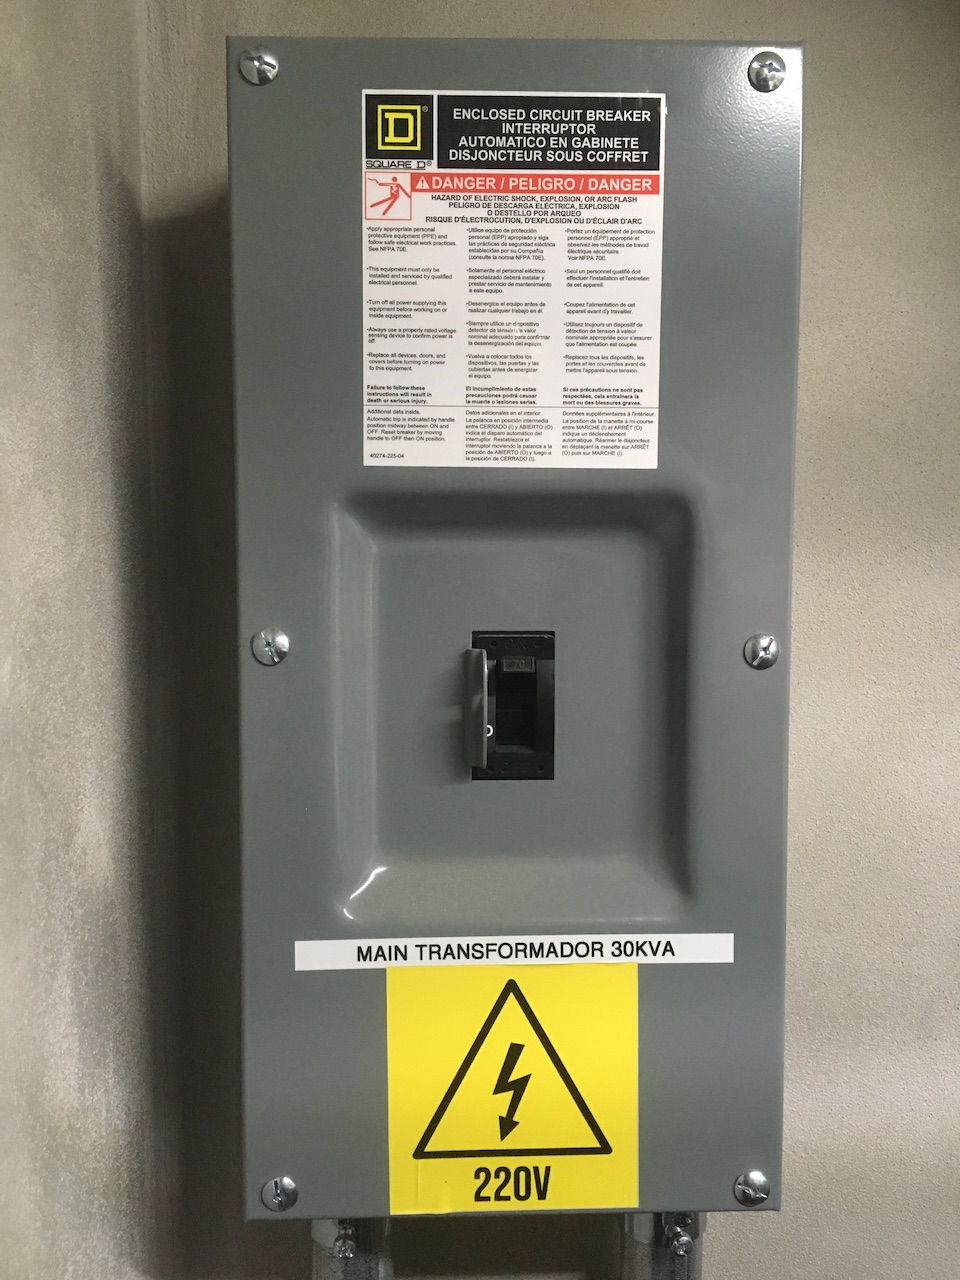
\includegraphics[width=0.45\linewidth,angle=0]{figures/electrical-power-ddoti-main-breaker-box.jpg}}
\arrowandlabel{(0.2,-1.0)}{(0,-5)}{north}{{\projectname} Main Breaker}
\end{labeled}
\end{center}
\caption{The main breaker box in shed.}
\label{figure:main-breaker-box}
\end{figure}
\fi

\section{Circuits}

\begin{figure}[t]
\ifcoatli
\begin{center}
\begin{labeled}{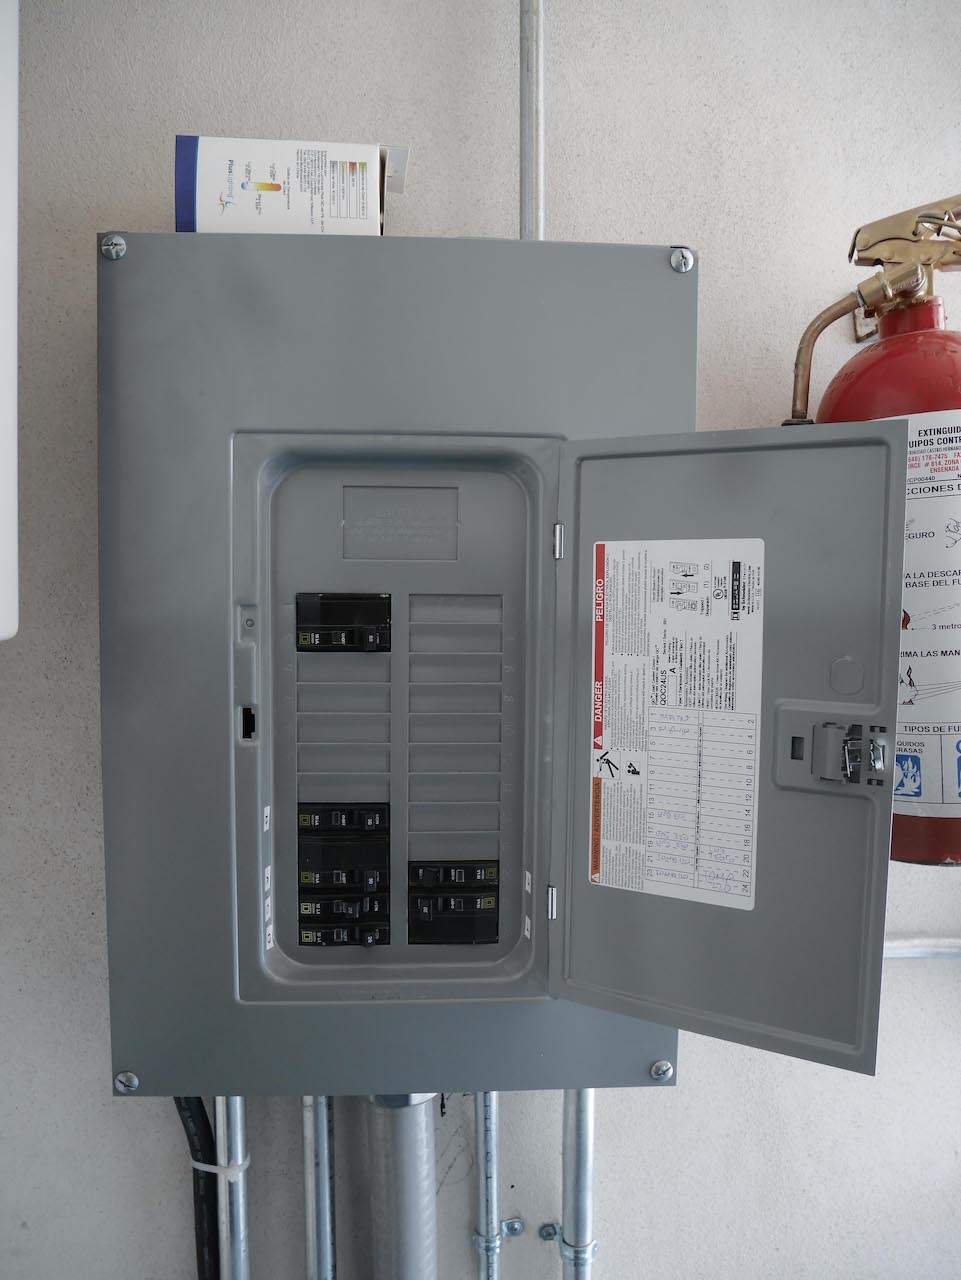
\includegraphics[height=0.7\linewidth]{figures/electrical-power-coatli-circuit-box.jpg}}
\arrowandlabel{(-0.7,0.5)}{(0,5)}{south}{Master Breaker}
\arrowandlabel{(-0.5,-2.2)}{(0,-5)}{north}{Breakers for Circuits A--F}
\end{labeled}
\end{center}
\caption{The circuit box the {\projectname} shed. The master breaker is at the top. The breakers for circuits A--F are at the bottom.}
\fi
\ifddoti
\begin{center}
\begin{labeled}{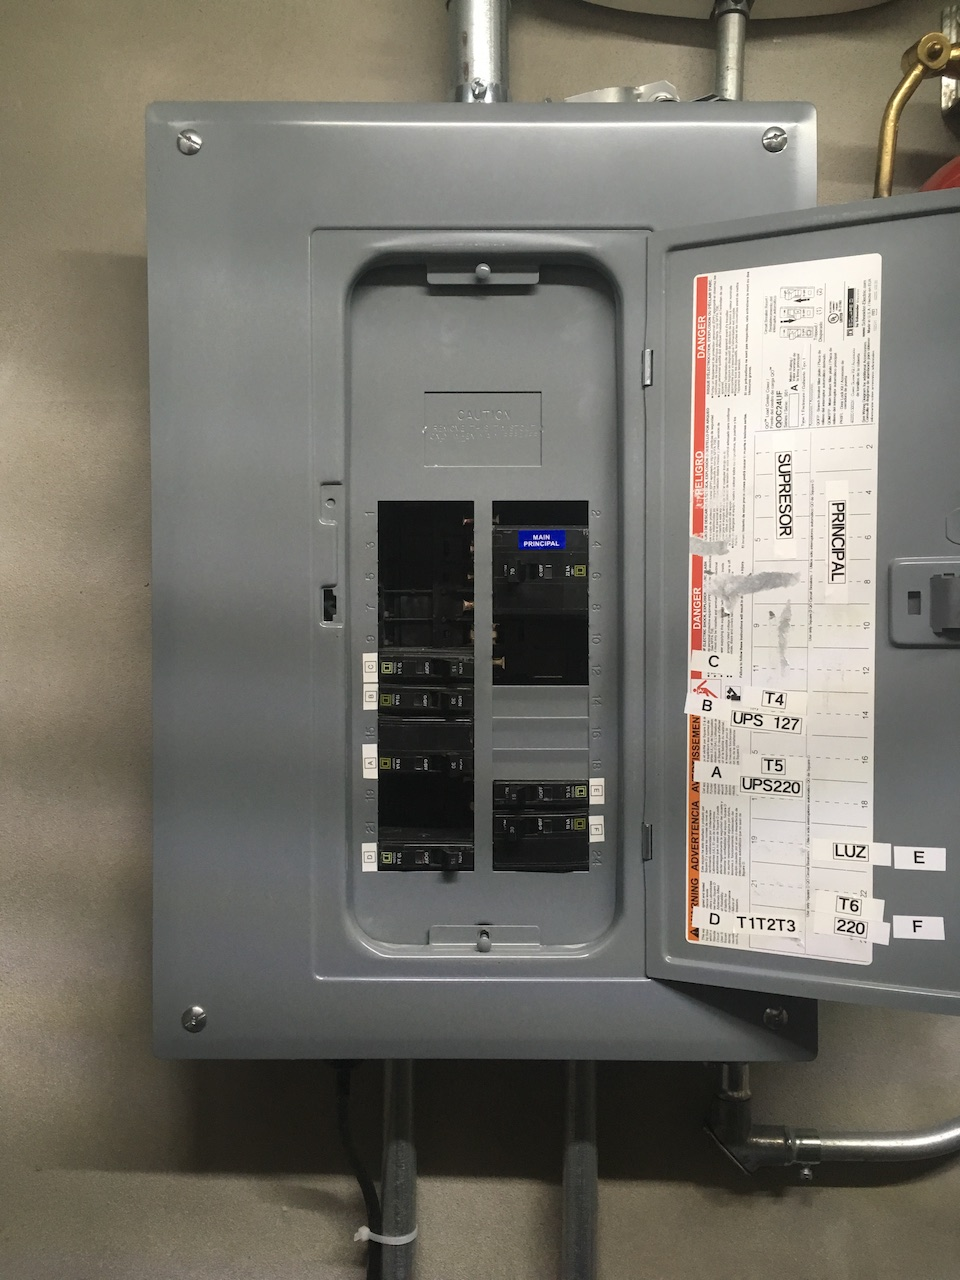
\includegraphics[width=0.45\linewidth,angle=0]{figures/electrical-power-ddoti-circuit-box.jpg}}
\arrowandlabel{(0.4,1)}{(0.5,5)}{south}{Master Breaker}
\arrowandlabel{(0,-1.7)}{(0,-5)}{north}{Breakers for Circuits A--F}
\end{labeled}
\end{center}
\caption{The circuit box the {\projectname} shed. The master breaker is at the top. The breakers for circuits A--F are at the bottom.}
\fi
\label{figure:circuit-box}
\end{figure}

Figure~\ref{figure:circuit-box} shows the circuit box in the shed. The master breaker is 80 A. The electricity supply is divided between the circuits listed in Table~\ref{table:circuits}, each with their own breaker. 

The 220~V circuits are generated between the two phases (L1 and L2). As a consequence, the 220~V circuits are live-live-ground, with 220~V between the two lives but each live 127~V above ground. (This is in contrast to a European-style live-neutral-ground 220~V circuit, with 220~V between live and neutral and with neutral nominally at the ground level.)

The 127~V circuits are generated between one of the two phases (L1 or L2) and the neutral (N). As a consequence, the 127~V circuits are live-neutral-ground, with 127~V between live and neutral and with neutral nominally at the ground level.

The wall sockets in the shed are labelled with their circuit.

Circuits A and B are regulated after the wall sockets by the two UPS units. The other circuits are unregulated. 

\begin{table*}
\caption{Circuits}
\label{table:circuits}
\begin{center}
\small
\resizebox{\columnwidth}{!}{
\begin{tabular}{lllll}
\hline
Circuit&Connection&Voltage&Breaker&Use\\
\hline
\ifcoatli
Master&L1-L2&220~V&80~A&Master for all circuits\\
A&L1-L2&220~V&30~A&Wall socket in shed for 220~V UPS (T5 $1\times$ NEMA L6-20R)\\
B&L2-N&127~V&30~A&Wall socket in shed for 127~V UPS (T4 $1\times$ NEMA L5-30R)\\
C&L1-N&127~V&20~A&Platform\\
D&L2-N&127~V&20~A&Wall sockets in shed (T0/T1/T2/T3 $2\times$ NEMA 5-15R)\\
E&L2-N&127~V&20~A&Lights in shed\\
F&L1-L2&220~V&30~A&Wall socket in shed (T6 $1\times$ NEMA L6-20R)\\
\fi
\ifddoti
Master&&220~V&70~A&Master for all circuits\\
A&L1-L2&220~V&30~A&Wall socket in shed for 220~V UPS (T5 $1\times$ NEMA L6-20R)\\
B&L2-N&127~V&30~A&Wall socket in shed for 127~V UPS (T4 $1\times$ NEMA L5-30R)\\
C&L1-N&127~V&15~A&Platform\\
D&L2-N&127~V&15~A&Wall sockets in shed (T1/T2/T3 $2\times$ NEMA 5-15R)\\
E&L2-N&127~V&15~A&Lights in shed\\
F&L1-L2&220~V&30~A&Wall socket in shed (T6 $1\times$ NEMA L6-20R)\\
\fi
\hline
\end{tabular}
}
\end{center}
\end{table*}

\section{UPS Units}

There are two UPS units in the rack in the shed. Both are Eaton 9310 models with nominal capacities of 3000~VA or 2700 W. Each is equipped with an external battery module, which extends the capacity to about 20 minutes of supply at full load.

\subsection{220~V UPS}

\begin{figure*}
\begin{center}
\footnotesize 
\resizebox{\columnwidth}{!}{
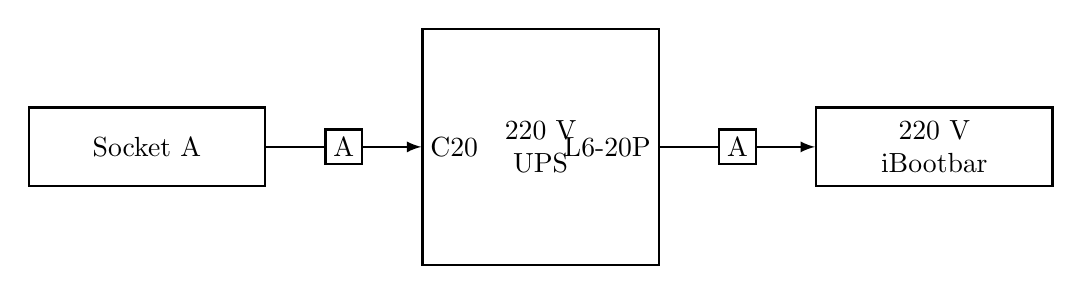
\begin{tikzpicture}
[
 thick,
 >={latex},
 align=center,
 inner sep=1mm,
 box/.style={draw=black,rectangle,minimum height=1cm,minimum width=3cm},
 main/.style={draw=black,rectangle,minimum width=3cm,minimum height=3cm},
 circuit/.style={draw=black,rectangle,fill=white}
]
\draw [white] (-6.5,0) -- (+6.5,0);
\node (ups-220) [main] at (0,0) {220 V\\ UPS};
\node (socket-a) at (-5,0) [box] {Socket A};
\node (ibb-220) at (+5,0) [box] {220 V\\iBootbar};
\draw[->] (socket-a) -- node [circuit] {A} (ups-220.west) node [right] {C20};
\draw[->] (ups-220.east) node [left] {L6-20P} -- node [circuit] {A} (ibb-220);
\end{tikzpicture}
}
\end{center}
\caption{Schematic of the Electrical Power Connections To and From the 220 V UPS}
\label{figure:schematic-electrical-power-box-ups-220}
\end{figure*}

The 220~V UPS is an Eaton PW9130G3000R-XL2U with PW9130N3000R-EBM2U external battery module. It is configured for 220~V 60~Hz input and output. Both the input and output are 220~V live-live-ground, with 220~V between the two lives and 127~V between each live and the ground.

Figure~\ref{figure:schematic-electrical-power-box-ups-220} shows a schematic of the electrical power connections.

The UPS is supplied via a NEMA L6-20P to C19 coupler connected to the NEMA L6-20R wall socket of circuit A and the C20 input socket of the UPS.

One of the NEMA L6-20R output sockets is connected to the 220~V iBootBar. No other output sockets are used.

If the UPS fails, it can be bypassed manually by connecting the NEMA L6-20P plug of the 220~V iBootBar to directly to the wall socket of circuit A.

\subsection{127~V UPS}

\begin{figure*}
\begin{center}
\footnotesize 
\resizebox{\columnwidth}{!}{
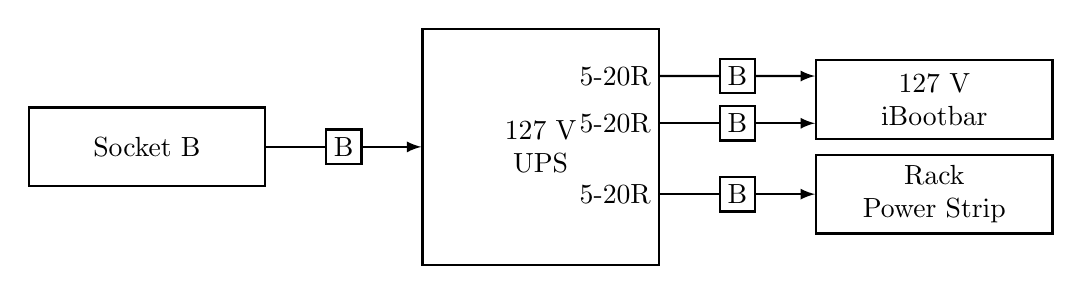
\begin{tikzpicture}[
 thick,
 >={latex},
 align=center,
 inner sep=1mm,
 box/.style={draw=black,rectangle,minimum height=1cm,minimum width=3cm},
 main/.style={draw=black,rectangle,minimum width=3cm,minimum height=3cm},
 circuit/.style={draw=black,rectangle,fill=white}
]
\draw [white] (-6.5,0) -- (+6.5,0);
\node (ups-127) [main] at (0,0) {127 V\\ UPS};
\node (socket-b) at (-5,0) [box] {Socket B};
\node (ibb-127) at (+5,+0.6) [box] {127 V\\iBootbar};
\node (rack-power-strip) at (+5,-0.6) [box] {Rack\\Power Strip};
\draw[->] (socket-b) -- node [circuit] {B} (ups-127);
\draw[->] 
 ($(ups-127.east) + (0,+0.9)$) node [left] {5-20R} 
 -- node [circuit] {B} 
 ($(ibb-127.west) + (0,+0.3)$);
\draw[->] 
 ($(ups-127.east) + (0,+0.3)$) node [left] {5-20R} 
 -- node [circuit] {B} 
 ($(ibb-127.west) + (0,-0.3)$);
\draw[->] 
 ($(ups-127.east) + (0,-0.6)$) node [left] {5-20R} 
 -- node [circuit] {B} 
 ($(rack-power-strip.west) + (0,0)$);
\end{tikzpicture}
}
\end{center}
\caption{Schematic of the Electrical Power Connections To and From the 127 V UPS}
\label{figure:schematic-electrical-power-box-ups-127}
\end{figure*}

The 127~V UPS is an Eaton PW9130L3000R-XL2U with PW9130N3000R-EBM2U external battery module. It is configured for 127~V 60~Hz input and output.

Figure~\ref{figure:schematic-electrical-power-box-ups-127} shows a schematic of the electrical power connections.

The UPS is supplied via a NEMA L5-30P plug connected to the NEMA L5-30R wall socket of circuit B.

Two of the NEMA 5-20R output sockets are connected to the NEMA 5-15P plugs of the 127~V iBootBar. Another NEMA 5-20R output socket is connected to the rack power strip. 

%The mount controller is \emph{not} connected via an iBootBar because it requires too much current. The power requirements of the mount controller are discussed on page 9 of the ASTELCO manual. The maximum draw in typical use is 400 W while tracking. However, it can use up to 1400 W when blocked. ASTELCO recommend fusing to 2500 W to cover the initial transient load. At 127 V, this corresponds to 20 A.
%The 127~V iBootBar is a 2N15-M model and can supply up to 12 A or 1500 W. This is insufficient for the initial transient.

If the UPS fails, it can be bypassed manually by connecting the two NEMA 5-15P plugs of the 127~V iBootBar directly to the wall sockets of circuit D.

\section{iBootBars}

There are two iBootBars in the rack in the shed, one 127~V and one 220~V. Both are the connected to the corresponding 127~V and 220~V UPS units. They are physically located in the rear of the rack towards the top.

\subsection{220~V iBootBar}

\begin{figure*}
\begin{center}
\footnotesize 
\resizebox{\columnwidth}{!}{
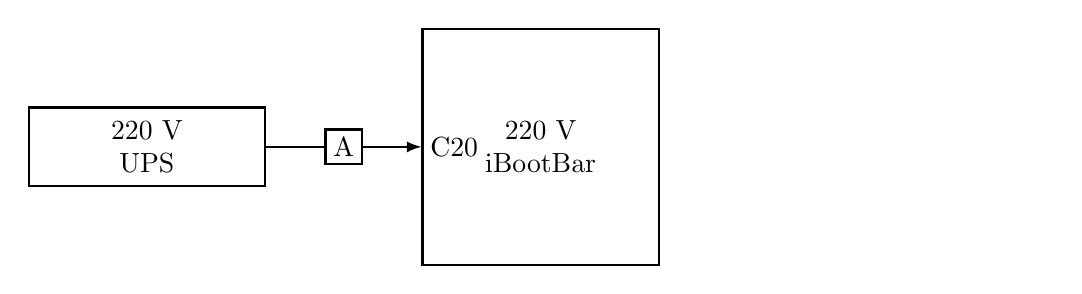
\begin{tikzpicture}
[
 thick,
 >={latex},
 align=center,
 inner sep=1mm,
 box/.style={draw=black,rectangle,minimum height=1cm,minimum width=3cm},
 main/.style={draw=black,rectangle,minimum width=3cm,minimum height=3cm},
 circuit/.style={draw=black,rectangle,fill=white}
]
\draw [white] (-6.5,0) -- (+6.5,0);
\node (ibb-220) [main] at (0,0) {220 V\\iBootBar};
\node (ups-220) at (-5,0) [box] {220 V\\UPS};
\ifcoatli
\node (secondary) at (5,+0.6) [box] {Secondary\\Controller};
\node (enclosure) at (5,-0.6) [box] {Enclosure\\Controller};
\draw[<-] (secondary.west) -- node [circuit] {A} +(-2,0) node [left] {F};
\draw[<-] (enclosure.west) -- node [circuit] {A} +(-2,0) node [left] {F};
\fi
\ifddoti
\node (enclosure) at (5,0) [box] {Enclosure\\Controller};
\draw[<-] (enclosure.west) -- node [circuit] {A} +(-2,0) node [left] {F};
\fi
\draw[->] (ups-220) -- node [circuit] {A} (ibb-220.west) node [right] {C20};
\end{tikzpicture}
}
\end{center}
\caption{Schematic of the Electrical Power Connections To and From the 220 V iBootBar}
\label{figure:schematic-electrical-power-box-ibb-220}
\end{figure*}

This is a DataProbe iBootBar iBB-C20. Figure~\ref{figure:schematic-electrical-power-box-ibb-220} shows a schematic of the electrical power connections.

The C20 input socket is connected to the 220~V UPS unit with a cable with C19 and NEMA L6-20P plugs.

The connections to the type F output sockets (“C13 female”) are given in Table~\ref{table:ibbs}. The iBootBar can supply up to 20~A.

The iBootBar is connected to the LAN at the address given in Table~\ref{table:network-addresses}. The HTTP and telnet account names and passwords are “{\projectaccount}” and “{\projectaccount}”. The HTTP interface is available from the {\projectname} web interface home page.

\subsection{127~V iBootBar}

\begin{figure*}
\begin{center}
\footnotesize 
\resizebox{\columnwidth}{!}{
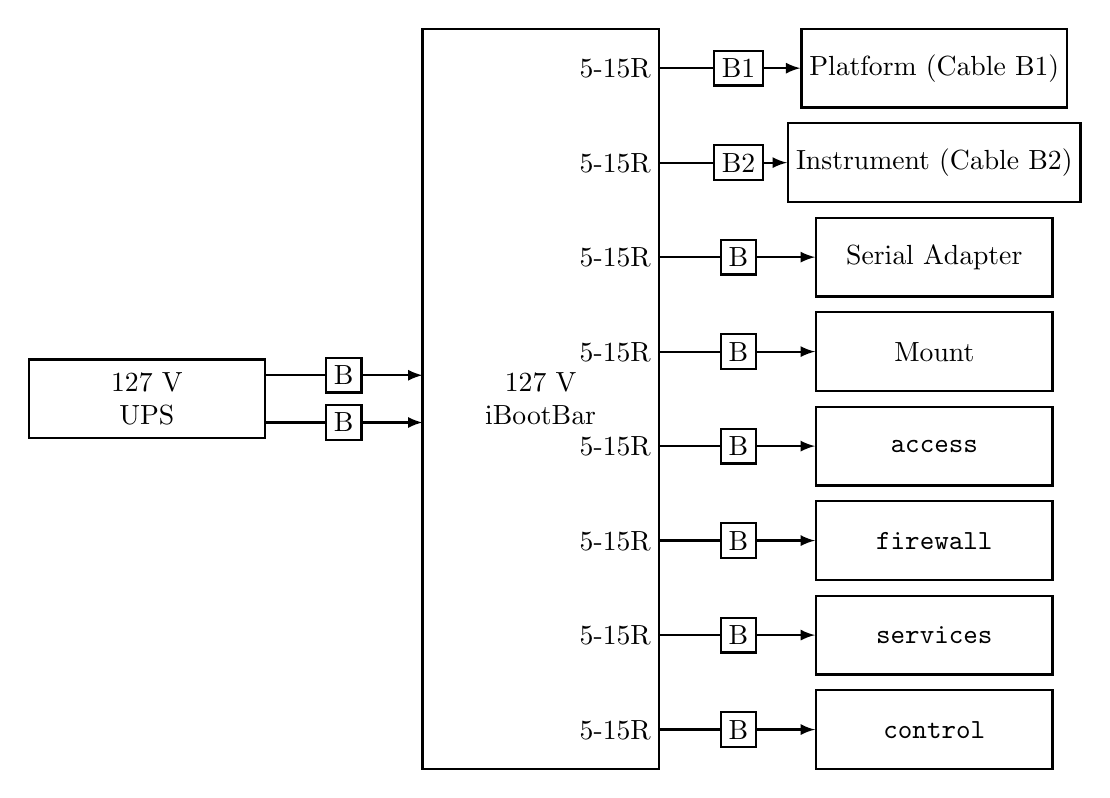
\begin{tikzpicture}
[
 thick,
 >={latex},
 align=center,
 inner sep=1mm,
 box/.style={draw=black,rectangle,minimum height=1cm,minimum width=3cm},
 main/.style={draw=black,rectangle,minimum width=3cm,minimum height=3cm},
 circuit/.style={draw=black,rectangle,fill=white}
]
\draw [white] (-6.5,0) -- (+6.5,0);
\node (ibb-127) [main,minimum height=9.4cm] at (0,0) {127 V\\iBootBar};
\node (ups-127) at (-5,0) [box] {127 V\\UPS};
\draw[->] (-3.5,+0.3) -- node [circuit] {B} (-1.5,+0.3);
\draw[->] (-3.5,-0.3) -- node [circuit] {B} (-1.5,-0.3);
\node (cable-b1) [box] at (5,+4.2) {Platform (Cable B1)};
\node (cable-b2) [box] at (5,+3.0) {Instrument (Cable B2)};
\node (serial) [box] at (5,+1.8) {Serial Adapter};
\node (mount) [box] at (5,+0.6) {Mount};
\node (access) [box] at (5,-0.6) {\ttfamily access};
\node (firewall) [box] at (5,-1.8) {\ttfamily firewall};
\node (services) [box] at (5,-3.0) {\ttfamily services};
\node (control) [box] at (5,-4.2) {\ttfamily control};

\draw[->] 
 ($(ibb-127.east) + (0,4.2)$) node [left] {5-15R} 
 -- ++(1,0) node [circuit] {B1} 
 |- (cable-b1.west);
\draw[->]
($(ibb-127.east) + (0,+3.0)$) node [left] {5-15R} 
 -- ++(1,0) node [circuit] {B2} 
 |- (cable-b2.west);
\draw[->] 
 ($(ibb-127.east) + (0,+1.8)$) node [left] {5-15R} 
 -- ++(1,0) node [circuit] {B} 
 |- (serial.west);
\draw[->] 
 ($(ibb-127.east) + (0,+0.6)$) node [left] {5-15R} 
 -- ++(1,0) node [circuit] {B} 
 |- (mount.west);
\draw[->] 
 ($(ibb-127.east) + (0,-0.6)$) node [left] {5-15R} 
 -- ++(1,0) node [circuit] {B} 
 |- (access.west);
\draw[->] 
 ($(ibb-127.east) + (0,-1.8)$) node [left] {5-15R} 
 -- ++(1,0) node [circuit] {B} 
 |- (firewall.west);
\draw[->] 
 ($(ibb-127.east) + (0,-3.0)$) node [left] {5-15R} 
 -- ++(1,0) node [circuit] {B} 
 |- (services.west);
\draw[->] 
 ($(ibb-127.east) + (0,-4.2)$) node [left] {5-15R} 
 -- ++(1,0) node [circuit] {B} 
 |- (control.west);
\end{tikzpicture}
}
\end{center}
\caption{Schematic of the Electrical Power Connections To and From the 127 V iBootBar}
\label{figure:schematic-electrical-power-box-ibb-127}
\end{figure*}

This is a DataProbe iBootBar iBB-2N15-M.  Figure~\ref{figure:schematic-electrical-power-box-ibb-127} shows a schematic of the electrical power connections.

The two NEMA 5-15P input plugs are connected to the 127~V UPS unit. 

The connections to the NEMA 5-15R output sockets are given in Table~\ref{table:ibbs}. The iBootBar can supply up to 15~A to each bank of four output sockets.

The iBootBar is connected to the LAN at the address given in Table~\ref{table:network-addresses}. The HTTP and telnet account names and passwords are “{\projectaccount}” and “{\projectaccount}”. The HTTP interface is available from the {\projectname} web interface home page.

The modem facility is not used.

TODO: Configure watchdog.

\begin{table*}
\caption{iBootBar Output Sockets}
\label{table:ibbs}
\begin{center}
\begin{tabular}{lll}
\hline
Socket&220~V iBootBar&127~V iBootBar\\
\hline
1&Enclosure&Platform (Cable B1)\\
2&
\ifcoatli
Secondary
\fi
\ifddoti
-
\fi
&\verb|access|\\
3&-&Instrument (Cable B2)\\
5&-&Mount\\
5&-&\verb|firewall|\\
6&-&\verb|services|\\
7&-&\verb|control|\\
8&-&\verb|serial|\\
\hline
\end{tabular}
\end{center}
\end{table*}

\section{Rack Power Strip}

%\begin{figure*}
%\begin{center}
%\footnotesize 
%\resizebox{\columnwidth}{!}{
%\begin{tikzpicture}
%[
% thick,
% >={latex},
% align=center,
% inner sep=1mm,
% box/.style={draw=black,rectangle,minimum height=1cm,minimum width=3cm},
% main/.style={draw=black,rectangle,minimum width=3cm,minimum height=3cm},
% circuit/.style={draw=black,rectangle,fill=white}
%]
%\draw [white] (-6.5,0) -- (+6.5,0);
%\node (power-strip) [main] at (0,0) {Power\\Strip};
%\node (ibb-127) at (-5,0) [box] {127 V\\iBootBar};
%\draw[->] (ibb-127) -- node [circuit] {B} (power-strip);
%
%\node (fiber-adapter) [box] at (5,+3.6) {Fiber Adapter};
%\node (time-capsule) [box] at (5,+2.4) {Time Capsule};
%\node (switch) [box] at (5,+1.2) {Switch};
%\node (control-mac) [box] at (5,+0.0) {Control Mac};
%\node (data-mac) [box] at (5,-1.2) {Data Mac};
%\node (pc) [box] at (5,-2.4) {PC};
%\node (monitor) [box] at (5,-3.6) {Monitor};
%\draw[->] 
% ($(power-strip.east) + (0,+1.2)$) node [left] {5-15R} 
% -- +(0.5,0) node [circuit] {B} 
% -- +(1.0,0) 
% |- (fiber-adapter.west);
%\draw[->] 
% ($(power-strip.east) + (0,+0.8)$) node [left] {5-15R} 
% -- +(1.0,0) node [circuit] {B} 
% -- +(1.3,0) 
% |- (time-capsule.west);
%\draw[->] 
% ($(power-strip.east) + (0,+0.4)$) node [left] {5-15R} 
% -- +(0.5,0) node [circuit] {B} 
% -- +(1.6,0) 
% |- (switch.west);
%\draw[->] 
% ($(power-strip.east) + (0,+0.0)$) node [left] {5-15R} 
% -- +(1.0,0) node [circuit] {B} 
% -- (control-mac.west);
%\draw[->] 
% ($(power-strip.east) + (0,-0.4)$) node [left] {5-15R} 
% -- +(0.5,0) node [circuit] {B} 
% -- +(1.6,0) 
% |- (data-mac.west);
%\draw[->] 
% ($(power-strip.east) + (0,-0.8)$) node [left] {5-15R} 
% -- +(1.0,0) node [circuit] {B} 
% -- +(1.3,0) 
% |- (pc.west);
%\draw[->] 
% ($(power-strip.east) + (0,-1.2)$) node [left] {5-15R} 
% -- +(0.5,0) node [circuit] {B} 
% -- +(1.0,0) 
% |- (monitor.west);
%\end{tikzpicture}
%}
%\end{center}
%\caption{Schematic of the Electrical Power Connections To and From the Rack Power Strip}
%\label{figure:schematic-electrical-power-rack-power-strip}
%\end{figure*}

At the rear of the rack, adjacent to the 127~V iBootBar, is a 8-way NEMA 5-15R power strip. The power strip powers the computers and network equipment in the rack. The entire power strip, and hence all of the connected equipment, is directly supplied by the 127~V UPS.

%Figure~\ref{figure:schematic-electrical-power-rack-power-strip} shows a schematic of the electrical power connections.


%\section{Box A}
%
%\begin{figure*}
%\begin{center}
%\footnotesize 
%\resizebox{\columnwidth}{!}{
%\begin{tikzpicture}[
% thick,
% >={latex},
% align=center,
% inner sep=1mm,
% box/.style={draw=black,rectangle,minimum height=1cm,minimum width=3cm},
% main/.style={draw=black,rectangle,minimum width=3cm,minimum height=3cm},
% circuit/.style={draw=black,rectangle,fill=white}
%]
%\draw [white] (-6.5,0) -- (+6.5,0);
%\node (box-a) [main] at (0,0) {Box A};
%\node (ibb-127) at (-5,+0.0) [box] {127 V\\iBootBar};
%\draw[->] (ibb-127.east) -- node [circuit] {B} +(2,0) node [right] {C14};
%\end{tikzpicture}
%}
%\end{center}
%\caption{Schematic of the Electrical Power Connections To Box A}
%\label{figure:schematic-electrical-power-box-a}
%\end{figure*}
%
%Box A is a smart control box located in the shed.  Figure~\ref{figure:schematic-electrical-power-box-a} shows a schematic of the electrical power connections to Box A.
%
%Box A is connected to circuit B, which powers the electronics, internal heater, and internal fans in Box A. 
%
%The connection to circuit B is via a NEMA 5-15P to C13 cable. The NEMA 5-15P plug is connected to an output socket of the 127 V iBootBar and the C13 plug is connected to the C14 input socket on Box A.
%
%Circuit B is switched and fuzed with a 1~A fuze at the entrance to Box A.

\begin{table*}
\caption{Fuzes}
\label{table:fuzes}
\begin{center}
\begin{tabular}{lcc}
\hline
Location&Circuit&Fuze\\
\hline
\ifcoatli
Power Box&B1\phantom{}&\phantom{0}3 A\\
Power Box&B2\phantom{}&\phantom{0}3 A\\
Power Box&C\phantom{0}&\phantom{}15 A\\
Platform Box&B1\phantom{}&\phantom{0}3 A\\
Instrument Box&B2\phantom{}&\phantom{0}3 A\\
\fi
\ifddoti
Power Box&B1\phantom{}&\phantom{0}3 A\\
Power Box&B2\phantom{}&\phantom{}15 A\\
Power Box&C\phantom{0}&\phantom{}15 A\\
Platform Box&B1\phantom{}&\phantom{0}3 A\\
Instrument0 Box&B2\phantom{}&\phantom{0}3 A\\
Instrument1 Box&B2\phantom{}&\phantom{0}3 A\\
\fi
\hline
\end{tabular}
\end{center}
\end{table*}


\section{Power Box}

\begin{figure*}
\begin{center}
\footnotesize 
\resizebox{\columnwidth}{!}{
\begin{tikzpicture}[
 thick,
 >={latex},
 align=center,
 inner sep=1mm,
 box/.style={draw=black,rectangle,minimum height=1cm,minimum width=3cm},
 main/.style={draw=black,rectangle,minimum width=3cm,minimum height=3cm},
 circuit/.style={draw=black,rectangle,fill=white}
]
\draw [white] (-6.5,0) -- (+6.5,0);
\ifcoatli
\node (power-box) [main,minimum height=5.8cm] at (0,0) {Power Box};
\fi
\ifddoti
\node (power-box) [main,minimum height=4.6cm] at (0,0) {Power Box};
\fi
\node (ibb-127) at (-5,+0.6) [box] {127 V\\iBootBar};
\node (circuit-box) at (-5,-0.6) [box] {Circuit Box};
\draw[->] (-3.5,+0.9) -- node [circuit] {B1} +(+2,0);
\draw[->] (-3.5,+0.3) -- node [circuit] {B2} +(+2,0);
\draw[->] (circuit-box.east) -- node [circuit] {C} +(+2,0);
\node at ($(power-box.north) + (-0.5,0)$) [below] {5-15R};
\node at ($(power-box.north) + (+0.5,0)$) [below] {5-15R};
\node at ($(power-box.north) + (0,-0.4)$) [below] {Sockets C};
\ifcoatli
\node (instrument1-box) at (+5,+2.4) [box] {Box E};
\node (instrument-box) at (+5,+1.2) [box] {Box D};
\node (platform-box) at (+5,+0.0) [box] {Platform Box};
\node (manual-light) at (+5,-1.2) [box] {Manual Light};
\node (emergency-light) at (+5,-2.4) [box] {Emergency Light};
\fi
\ifddoti
\node (platform-box) at (+5,+0.6) [box] {Platform Box};
\node (instrument0-box) at (+5,+1.8) [box] {Instrument0 Box};
\node (instrument1-box) at (+5,+3.0) [box] {Instrument1 Box};
\node (manual-light) at (+5,-0.6) [box] {Manual Light};
\node (emergency-light) at (+5,-1.8) [box] {Emergency Light};
\draw[<-] (instrument0-box.west) -- +(-1,0) node [circuit] {B2} -- +(-2,0);
\draw[->] (instrument0-box.east) -- +(0.4,0) -- node [circuit] {B2} +(0.4,+1.2) |- (instrument1-box.east);
\fi
\ifcoatli
\draw[<-] (instrument-box.west) -- +(-1,0) node [circuit] {B1} -- +(-2,0);
\fi
\draw[<-] ($(platform-box.west) + (0,+0.3)$) -- +(-1,0) node [circuit] {B1} -- +(-2,0);
\draw[<-] ($(platform-box.west) + (0,-0.3)$) -- +(-1,0) node [circuit] {C} -- +(-2,0);
\draw[<-] (manual-light.west) -- +(-1,0) node [circuit] {C} -- +(-2,0);
\draw[<-] (emergency-light.west) -- +(-1,0) node [circuit] {C} -- +(-2,0);
\end{tikzpicture}
}
\end{center}
\caption{Schematic of the Electrical Power Connections To and From the Power Box}
\label{figure:schematic-electrical-power-power-box}
\end{figure*}

The power box is a dumb electrical distribution box located on the platform.  Figure~\ref{figure:schematic-electrical-power-power-box} shows a schematic of the electrical power connections to Power Box.

The power box is connected to circuits B1, B2, and C. Circuits B1 and B2 are subcircuits of circuit B. Circuit B1 is used to power electronics, internal heaters, and internal fans in Boxes C and D, the two other boxes on the platform. Circuit B2 is used for power the electronics, internal heaters, and internal fans in Box E on the telescope. Circuit C is used to power the two NEMA 5-15R plugs on the power box (for general use), the three lights on the platform (one with manual control, one with manual/electronic control, and one emergency), and the external heater on the platform.

The connection to circuits B1 and B2 are via cables with NEMA 5-15P plugs connected to the 127~V iBootBar. 

The connection to circuit C is hardwired to the circuit box in the shed. The connections are hardwired at the power box.

The three circuits are switched and fuzed (see Table~\ref{table:fuzes}) at the entrance to the power box.

The manually-controlled light is hardwired to the platform box and has a manual switch on the power box.

\section{Platform Box}

\begin{figure*}
\begin{center}
\footnotesize 
\resizebox{\columnwidth}{!}{
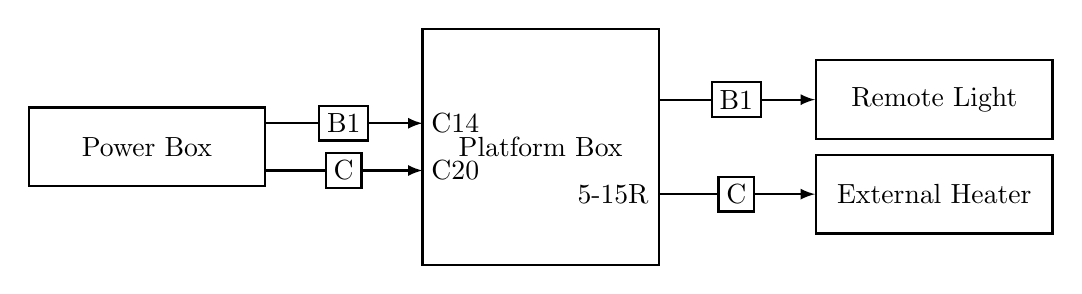
\begin{tikzpicture}[
 thick,
 >={latex},
 align=center,
 inner sep=1mm,
 box/.style={draw=black,rectangle,minimum height=1cm,minimum width=3cm},
 main/.style={draw=black,rectangle,minimum width=3cm,minimum height=3cm},
 circuit/.style={draw=black,rectangle,fill=white}
]
\draw [white] (-6.5,0) -- (+6.5,0);
\node (platform-box) [main] at (0,0) {Platform Box};
\node (power-box) [box] at (-5,0) {Power Box};
\node (light) at (+5,+0.6) [box] {Remote Light};
\node (heater) at (+5,-0.6) [box] {External Heater};
\draw[->] (-3.5,+0.3) -- node [circuit] {B1} +(2,0) node [right] {C14};
\draw[->] (-3.5,-0.3) -- node [circuit] {C} +(2,0) node [right] {C20};
\draw[<-] (light.west) -- node [circuit] {B1} +(-2,0);
\draw[<-] (heater.west) -- node [circuit] {C} +(-2,0) node [left] {5-15R};
\end{tikzpicture}
}
\end{center}
\caption{Schematic of the Electrical Power Connections To and From the Platform Box}
\label{figure:schematic-electrical-power-platform-box}
\end{figure*}

The platform box is a smart control box located on the platform. Figure~\ref{figure:schematic-electrical-power-platform-box} shows a schematic of the electrical power connections to the platform box.


The platform box is connected to circuits B1 and C. Circuit B1 is a subcircuit of circuit B. Circuit B1 is used to power the electronics, the internal heater, and the internal fans. Circuit C is used to power an external light and the external heater on the platform.

The connection to circuit B1 is via a cable with a C13 plug that connects to the C14 input socket on the platform box. The cable is hardwired to the power box.

The connection to circuit C is via a cable with a C19 plug that connects to the C20 input socket on the platform box. The cable is hardwired to the power box.

The connections to the manually/electronically-controlled light and heater are via the two NEMA 5-15R sockets on the platform box. The light is controlled both by a relay and by a manual switch on the platform box (with the light being on if either the relay or manual switch are on). The heater is controlled by a relay.

Circuit B1 is switched and fuzed (see Table~\ref{table:fuzes}) at the entrance to the platform box.

\ifcoatli

\section{Instrument Box}

\begin{figure*}
\begin{center}
\footnotesize 
\resizebox{\columnwidth}{!}{
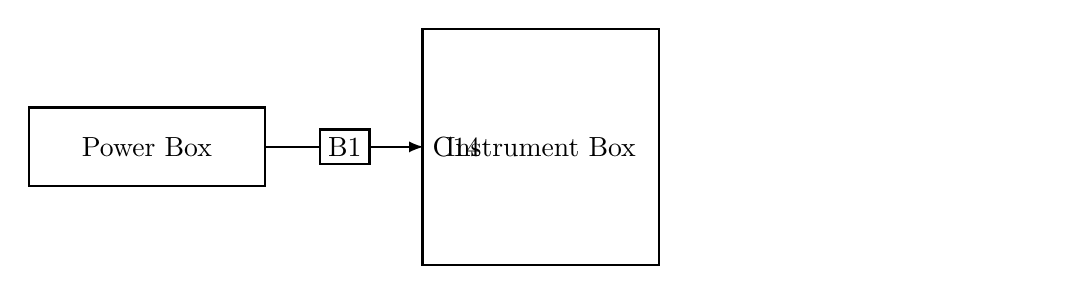
\begin{tikzpicture}[
 thick,
 >={latex},
 align=center,
 inner sep=1mm,
 box/.style={draw=black,rectangle,minimum height=1cm,minimum width=3cm},
 main/.style={draw=black,rectangle,minimum width=3cm,minimum height=3cm},
 circuit/.style={draw=black,rectangle,fill=white}
]
\draw [white] (-6.5,0) -- (+6.5,0);
\node (instrument-box) [main] at (0,0) {Instrument Box};
\node (power-box) [box] at (-5,0) {Power Box};
\draw[->] (power-box.east) -- node [circuit] {B1} +(2,0) node [right] {C14};
\end{tikzpicture}
}
\end{center}
\caption{Schematic of the Electrical Power Connections To Instrument Box}
\label{figure:schematic-electrical-power-instrument-box}
\end{figure*}

The instrument box is a smart control box located on the platform. Figure~\ref{figure:schematic-electrical-power-instrument-box} shows a schematic of the electrical power connections to Box D.

The instrument nox is connected to circuit B1. Circuit B1 is a subcircuit of circuit B. Circuit B1 is used to power the electronics, the internal heater, and the internal fans.

The connection to circuit B1 is via a cable with a C13 plug that connects to the C14 input socket on the platform box. The cable is hardwired to the power box.

Circuit B1 is switched and fuzed (see Table~\ref{table:fuzes}) at the entrance to the instrument box.

\section{Box E}

\begin{figure*}
\begin{center}
\footnotesize 
\resizebox{\columnwidth}{!}{
\begin{tikzpicture}[
 thick,
 >={latex},
 align=center,
 inner sep=1mm,
 box/.style={draw=black,rectangle,minimum height=1cm,minimum width=3cm},
 main/.style={draw=black,rectangle,minimum width=3cm,minimum height=3cm},
 circuit/.style={draw=black,rectangle,fill=white}
]
\draw [white] (-6.5,0) -- (+6.5,0);
\node (instrument1-box) [main] at (0,0) {Box E};
\node (power-box) [box] at (-5,0) {Power Box};
\draw[->] (power-box.east) -- node [circuit] {B2} +(2,0) node [right] {C14};
\end{tikzpicture}
}
\end{center}
\caption{Schematic of the Electrical Power Connections To Box E}
\label{figure:schematic-electrical-power-instrument1-box}
\end{figure*}

Box E is a smart control box located on the pillar of the COATLI telescope. Figure~\ref{figure:schematic-electrical-power-instrument1-box} shows a schematic of the electrical power connections to Box E.

Box E is connected to circuit B2. Circuit B2 is a subcircuit of circuit B. Circuit B2 is used to power the electronics, the internal heater, and the internal fans.

The connection to circuit B2 is via a cable with a C13 plug that connects to the C14 input socket on Box E. The cable is hardwired to the power box.

Circuit B2 is switched and fuzed (see Table~\ref{table:fuzes}) at the entrance to Box E.

\fi

\ifddoti

\section{Instrument0 Box}

\begin{figure*}
\begin{center}
\footnotesize 
\resizebox{\columnwidth}{!}{
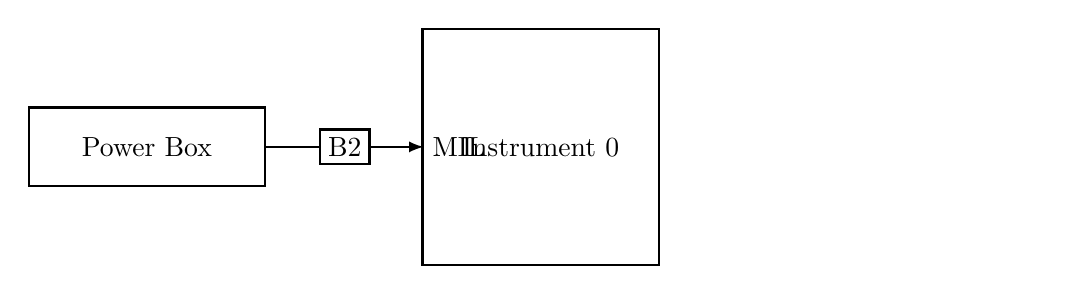
\begin{tikzpicture}[
 thick,
 >={latex},
 align=center,
 inner sep=1mm,
 box/.style={draw=black,rectangle,minimum height=1cm,minimum width=3cm},
 main/.style={draw=black,rectangle,minimum width=3cm,minimum height=3cm},
 circuit/.style={draw=black,rectangle,fill=white}
]
\draw [white] (-6.5,0) -- (+6.5,0);
\node (instrument0-box) [main] at (0,0) {Instrument 0};
\node (instrument1-box) [box] at (-5,0) {Power Box};
\draw[->] (instrument1-box.east) -- node [circuit] {B2} +(2,0) node [right] {MIL};
\end{tikzpicture}
}
\end{center}
\caption{Schematic of the Electrical Power Connections To The Instrument0 Box}
\label{figure:schematic-electrical-power-instrument0-box}
\end{figure*}

The instrument0 box is a smart control box located on the DDOTI telescopes. Figure~\ref{figure:schematic-electrical-power-instrument0-box} shows a schematic of the electrical power connections to the instrument0 box.

The instrument 0 box is connected to circuit B2. Circuit B2 is a subcircuit of circuit B. Circuit B2 is used to power the electronics, the internal heater, and the internal fans.

The connection to circuit B2 is via a cable with a MIL plug that connects to the MIL input socket on Box D. The cable is hardwired to the power box. The cable passes from the power box up onto the telescope through the mount and the custom connector.

Circuit B2 is switched and fuzed (see Table~\ref{table:fuzes}) at the entrance to the instrument0 box.

\section{The Instrument1 Box}

\begin{figure*}
\begin{center}
\footnotesize 
\resizebox{\columnwidth}{!}{
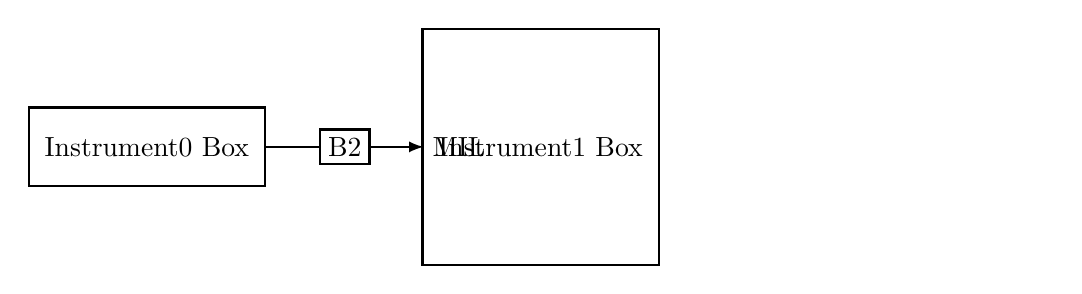
\begin{tikzpicture}[
 thick,
 >={latex},
 align=center,
 inner sep=1mm,
 box/.style={draw=black,rectangle,minimum height=1cm,minimum width=3cm},
 main/.style={draw=black,rectangle,minimum width=3cm,minimum height=3cm},
 circuit/.style={draw=black,rectangle,fill=white}
]
\draw [white] (-6.5,0) -- (+6.5,0);
\node (instrument1-box) [main] at (0,0) {Instrument1 Box};
\node (instrument0-box) [box] at (-5,0) {Instrument0 Box};
\draw[->] (instrument0-box.east) -- node [circuit] {B2} +(2,0) node [right] {MIL};
\end{tikzpicture}
}
\end{center}
\caption{Schematic of the Electrical Power Connections To Instrument1 Box}
\label{figure:schematic-electrical-power-instrument1-box}
\end{figure*}

The instrument1 box is a smart control box located on the pillar of the COATLI telescope. Figure~\ref{figure:schematic-electrical-power-instrument1-box} shows a schematic of the electrical power connections to Box E.

The instrument1 box is connected to circuit B2. Circuit B2 is a subcircuit of circuit B. Circuit B2 is used to power the electronics, the internal heater, and the internal fans.

The connection to circuit B2 is via a cable with a MIL plug that connects to the MIL input socket on the instrument1 box. The cable passes through the mount declination bearing to the instrument0 box and has an inline C13/C14 connector close to instrument0 box to allow instrument0 to be demounted.

Circuit B2 is switched and fuzed (see Table~\ref{table:fuzes}) at the entrance to Box E.

\fi

\section{Trouble-Shooting}

\begin{itemize}
\item Check cables. Has one been disconnected or worked itself lose?
\item Check switches. Is the equipment switched on? The smart boxes have switch for their regulated input (circuits B, B1, or B2). The power box has switches for circuits B1, B2, and C. The Macs and the PC have power switches. The ASTELCO equipment has power switches.
\item Check fuzes. Has one blown? See Table~\ref{table:fuzes}.
\item For circuits connected via an iBootBar (A, B, B1, and B2), check that the corresponding output socket is on. The state of the output sockets is given by the row of 8 green LEDs on the front of each iBootBar.
\item The emergency lights come on if the corresponding circuit (C for the platform and E for the shed) has no power. This can happen because a breaker trips or because the OAN mains supply has failed.
\item For circuits not connected via a UPS unit (C, D, E, and F), check that the OAN mains supply is working.
\item For circuits connected via a UPS unit (A, B, B1, and B2), check that the corresponding UPS is working.
\item Check the breakers in the circuit box in the shed. Has one tripped?
\ifcoatli
\item Check the breaker in the main breaker box in the 84-cm. Has it tripped?
\fi
\ifddoti
\item Check the breaker in the main breaker box. Has it tripped?
\fi
\item Check the equipment has not failed.
\end{itemize}

\section{Bibliography}

\begin{flushleft}
\begin{itemize}
\item “\href{bibliography/eaton-9130-ups.pdf}{Eaton 9300 UPS 700/3000~VA User's Guide}” (Revision 8)
\item “\href{bibliography/dataprobe-ibootbar.pdf}{iBootBar Installations and Operations}” (Version 1.5)
\end{itemize}
\end{flushleft}


\chapter{Electrical Grounding}
\label{chapter:electrical-grounding}

This chapter describes the electrical grounding system in the {\projectname} installation. The electrical power system is described in Chapter~\ref{chapter:electrical-power}.

TODO: Measure DDOTI ground resistance.

\section{Grounding Rods}

\ifcoatli
We have installed a network of ground rods to the 
east of the 84-cm telescope building. There is one main rod and two delta or triad rod systems. The three systems are connected through a ground bar in a box on the eastern wall of the 84-cm telescope.

The 84-cm telescope building is grounded through an independent network of grounding rods just to the south of the building.
\fi

\ifddoti
We have installed a network of ground rods to the 
east of shed. There is one main rod and two delta or triad rod systems. The three systems are connected through a ground bar in a box on the eastern wall of shed.
\fi

TODO: Photo.


\section{Grounding System}

\ifcoatli
Figure~\ref{figure:schematic-electrical-grounding-system} shows a schematic of the electrical grounding system. These grounding cable from the grounding rods runs through the conduit from the 84-cm to the {\projectname} installation. It is terminated at a protected grounding bar underneath the metal walkway. This is the “tau-point” of the grounding system. From here, spurs are used to ground the electrical system in the shed, the walkways, the tower, and the platform.
\fi
\ifddoti
Figure~\ref{figure:schematic-electrical-grounding-system} shows a schematic of the electrical grounding system. These grounding cables from the grounding rods are connected at a protected grounding bar on the east side of the shed. This is the “tau-point” of the grounding system. From here, spurs are used to ground the electrical system in the shed, the tower, and the platform.
\fi

TODO: Photo of the tau-point.

TODO: Cable calibres.

\begin{figure*}
\begin{center}
\resizebox{\columnwidth}{!}{
\begin{tikzpicture}[
 thick,
 box/.style={
  inner sep=1mm,
  draw=black,
  rectangle,
  minimum width=2cm,
  minimum height=0.6cm,
  align=center
 }
] 

\node at (1.5,1.75) [right,align=left] {Ground\\Rods};

\begin{scope}[xshift=0cm,yshift=1.5cm]
\draw (-0.25,-0.0) -- (+0.25,-0.0);
\draw (-0.15,-0.1) -- (+0.15,-0.1);
\draw (-0.05,-0.2) -- (+0.05,-0.2);
\end{scope}
\begin{scope}[xshift=+1cm,yshift=1.5cm]
\draw (-0.25,-0.0) -- (+0.25,-0.0);
\draw (-0.15,-0.1) -- (+0.15,-0.1);
\draw (-0.05,-0.2) -- (+0.05,-0.2);
\end{scope}
\begin{scope}[xshift=-1cm,yshift=1.5cm]
\draw (-0.25,-0.0) -- (+0.25,-0.0);
\draw (-0.15,-0.1) -- (+0.15,-0.1);
\draw (-0.05,-0.2) -- (+0.05,-0.2);
\end{scope}

\draw (-1,1.5) -- (-1,2) -- (0,2);
\draw (+1,1.5) -- (+1,2) -- (0,2);
\draw (0,1.5) -- (0,2);

%\node at (0.2,2) [right] {Conduit};
%\draw (-0.2,1) -- (-0.1,1) -- (-0.1,3) -- (-0.2,3);
%\draw (+0.2,1) -- (+0.1,1) -- (+0.1,3) -- (+0.2,3);

\node (tao-point-ground-bar) at (0,4) [box,minimum width=11cm] {Tau-Point Ground Bar};

\draw (0,2) -- (tao-point-ground-bar);

\ifcoatli
\node (walkways) [box] at (-4.5,5.5) {Walkways};
\draw ($(tao-point-ground-bar.north) + (-4.5,0)$) -- (walkways);
\fi

\node (shed-ground-bar) at (-1.5,7.5) [box,minimum width=5 cm] {Shed Ground Bar};
\draw ($(tao-point-ground-bar.north) + (-1.5,0)$) -- (shed-ground-bar);

\node (tower) [box] at (+1.5,5.5) {Tower};
\draw ($(tao-point-ground-bar.north) + (+1.5,0)$) -- (tower);

\node (platform-ground-bar) at (4.5,11.5) [box,minimum width=5 cm] {Platform Ground Bar};
\draw ($(tao-point-ground-bar.north) + (+4.5,0)$) -| (platform-ground-bar.south);

\node (circuit-box) [box] at (-3.0,8.5) {Circuit Box};
\draw ($(shed-ground-bar.north) + (-1.5,0)$) -- (circuit-box.south);

\node (circuits-a-f) [box] at (-3.0,9.5) {Circuits A--F};
\draw (circuit-box) -- (circuits-a-f);

\node (rack-chassis) [box] at (+0.0,8.5) {Rack Chassis};
\draw ($(shed-ground-bar.north) + (+1.5,0)$) -- (rack-chassis.south);

\node (box-b) [box] at (3.0,12.5) {Box B};
\draw ($(platform-ground-bar.north) + (-1.5,0)$) -- (box-b.south);

\ifcoatli
\node (boxes) [box] at (3.0,13.5) {Boxes C/D/F};
\fi
\ifddoti
\node (boxes) [box] at (3.0,13.5) {Boxes C/D/E};
\fi
\draw (box-b) -- (boxes);

\node (mount) [box] at (6.0,12.5) {Mount};
\draw ($(platform-ground-bar.north) + (+1.5,0)$) -- (mount.south);

\draw[dashed] (-6,6.5) -- (+8,6.5);
\draw[dashed] (-6,10.5) -- (+8,10.5);
\draw[dashed] (-6,14.5) -- (+8,14.5);
\node at (-6,+8.5) [right] {\normalsize Shed};
\node at (-6,+12.5) [right] {\normalsize Platform};

\end{tikzpicture}
}
\end{center}
\caption{Schematic of the Electrical Grounding System}
\label{figure:schematic-electrical-grounding-system}
\end{figure*}

The ground bar in the shed is used to provide ground to circuit box and hence to the circuits and the sockets in the shed. It is also used to ground the rack.

Circuits B1, B2, and C run from the shed to Box B on the platform. However, their ground is not connected in Box B. Instead, the ground bar on the platform is used to provide ground for Box B and subsequently for the sockets on the platform (in boxes B and C), the cables to boxes C, D, E, and F, and the mount.

TODO: Make sure the ground is connected to the cables between the boxes.

The Astelco controllers in the shed are connected to the platform and mount. There are undoubtedly ground loops through these connections. However, the connections from the platform to the tau-point is through a heavy-gauge cable, and this is likely to mitigate these ground loops.

\ifcoatli

\section{Ground Resistance}

In October 2016 we measured a ground resistance of about 5.5~$\Omega$ at all three of the ground bars (the tau-point, shed ground bar, and platform ground bar) using the three-point method. We further measured a resistance of about 0.8~$\Omega$ between the grounding point of the NTM-500 mount and the platform grounding bar and between the ground contacts of the outlets of the iBootBars and the shed grounding bar. This suggests that the grounding system is working well.

\fi

\chapter{Network}
\label{chapter:network}

TODO: haltsoon and rebootsoon

\begin{figure*}
\begin{center}
\resizebox{!}{0.9\textheight}{
\begin{tikzpicture}
[
 thick,
 box/.style={
  draw,
  minimum height=1cm,
  minimum width=2cm,
  inner sep=1mm,
  align=center,
 }
]
 \footnotesize
 \node at (0,0) (internet) [box] {Internet};
 
 \draw[dashed] (-4.5,1.0) -- (+7.5,1.0) -- (+7.5,6.0) -- (-4.5,6.0) -- node [above,rotate=90] {84-cm} cycle;

 \node at (0,2.0) (oan-firewall) [box] {OAN/SPM\\Firewall};
 \ifcoatli
 \node at (3,3.5) (webcam-c) [box] {webcam-c\\132.148.4.16};
 \fi
 \ifddoti
 \node at (3,3.5) (webcam-c) [box] {webcam-c\\132.148.4.26};
 \fi
 \node at (0,3.5) (switch-84) [box] {Switch\\84-cm};
 \node at (0,5.0) (fiber-84) [box] {Fibre Adapter};
 
 \draw (internet) -- (oan-firewall);
 \draw (switch-84) -- (webcam-c);
 \draw (oan-firewall) -- (switch-84);
 \draw (switch-84) -- (fiber-84);

 \draw[dashed] (-4.5,6.5) -- (+7.5,6.5) -- (+7.5,13.0) -- (-4.5,13.0) -- node [above,rotate=90] {Shed} cycle;
 
 \node at (0,7.5) (fiber-shed) [box] {Fibre Adapter};
 \node at (0,9.0) (firewall) [box] {10.0.1.1\\firewall\\{\projectexternalipaddress}};
 \node at (0,10.5) (switch-rack) [box] {Switch\\Rack};

 \draw (fiber-84) -- (fiber-shed);
 \draw (fiber-shed) -- (firewall);
 \draw (firewall) -- (switch-rack);

 \node at (-3,12.0) (access) [box] {access\\10.0.1.2};
 \node at (-3,10.5) (services) [box] {services\\10.0.1.3};
 \node at (-3,9.0) (control) [box] {control\\10.0.1.9};
 \node at (+3,12.0) (ibb-220) [box] {ibb-220\\10.0.1.4}; 
 \node at (+3,9.0) (ibb-127) [box] {ibb-127\\10.0.1.5}; 
 \node at (+6,11.25) (mount) [box] {mount\\10.0.1.6};
 \node at (+6,9.75) (serial) [box] {serial\\10.0.1.7};
 
 \draw (switch-rack) -- (access);
 \draw (switch-rack) -- (services);
 \draw (switch-rack) -- (control);
 \draw (switch-rack) -- (ibb-127);
 \draw (switch-rack) -- (ibb-220);
 \draw (switch-rack) -- (mount);
 \draw (switch-rack) -- (serial);
 
 \draw[dashed] (-4.5,13.5) -- (+7.5,13.5) -- (+7.5,17.0) -- (-4.5,17.0) -- node [above,rotate=90] {Platform} cycle;

 \node at (0,15.25) (switch-c) [box] {Switch\\Box C};
 \node at (-3,14.5) (c0) [box] {c0\\10.0.1.11}; 
 \node at (-3,16.0) (airport-express) [box] {airport-express\\10.0.1.10}; 
 \draw (switch-c) -- (c0);
 \node at (+3,14.5) (webcam-a) [box] {webcam-a\\10.0.1.20}; 
 \node at (+3,16.0) (webcam-b) [box] {webcam-b\\10.0.1.21}; 
 \draw (switch-rack) -- (switch-c);
 \draw (switch-c) -- (webcam-a);
 \draw (switch-c) -- (webcam-b);
 \draw (switch-c) -- (airport-express);
 \ifcoatli
 \node at (+6,15.25) (d0) [box] {d0\\10.0.1.12}; 
 \draw (switch-c) -- (d0);
 \fi
 
 \ifcoatli 
 \draw[dashed] (-4.5,17.5) -- (+7.5,17.5) -- (+7.5,19.5) -- (-4.5,19.5) -- node [above,rotate=90] {Telescope} cycle;
 \node at (0,18.5) (switch-e) [box] {Switch\\Box E};
 \node at (-3,18.5) (e0) [box] {e0\\10.0.1.15}; 
 \node at (+3,18.5) (e1) [box] {e1\\10.0.1.16}; 
 \draw (switch-c) -- (switch-e);
 \draw (switch-e) -- (e0);
 \draw (switch-e) -- (e1);
 \fi

 \ifddoti 
 \draw[dashed] (-4.5,17.5) -- (+7.5,17.5) -- (+7.5,25.5) -- (-4.5,25.5) -- node [above,rotate=90] {Telescope} cycle;
 \node at (-3,20.5) (d0) [box] {d0\\10.0.1.12}; 
 \node at (-3,18.5) (d1) [box] {d1\\10.0.1.13}; 
 \node at (+3,20.5) (d2) [box] {d2\\10.0.1.14}; 
 \node at (+3,18.5) (d3) [box] {d3\\10.0.1.15}; 
 \node at (0,19.75) (switch-d) [box] {Switch\\Box D};
 \draw (switch-c) -- (switch-d);
 \draw (switch-d) -- (d0);
 \draw (switch-d) -- (d1);
 \draw (switch-d) -- (d2);
 \draw (switch-d) -- (d3);
 \node at (-3,24.5) (e0) [box] {e0\\10.0.1.16}; 
 \node at (-3,22.5) (e1) [box] {e1\\10.0.1.17}; 
 \node at (+3,24.5) (e2) [box] {e2\\10.0.1.18}; 
 \node at (+3,22.5) (e3) [box] {e3\\10.0.1.19}; 
 \node at (0,23.75) (switch-e) [box] {Switch\\Box E};
 \draw (switch-d) -- (switch-e);
 \draw (switch-e) -- (e0);
 \draw (switch-e) -- (e1);
 \draw (switch-e) -- (e2);
 \draw (switch-e) -- (e3);
 \fi
 
\end{tikzpicture}
}
\end{center}
\caption{Network Physical Topology}
\label{figure:network-topology}
\end{figure*}

\section{WAN and LAN Addresses}

The observatory uses 132.248.4/24 as a WAN. {\projectname} uses 10.0.1/24 as a LAN. The firewall computer in the rack in the shed serves as a firewall and router between the WAN and the LAN. The addresses of the equipment are given in Table~\ref{table:network-addresses}.

\begin{table}
\caption{Addresses}
\label{table:network-addresses}
\begin{center}
\footnotesize
\begin{tabular}{llll}
\hline
Address&Name&Equipment&Location\\
\hline
{\projectexternalipaddress}&\verb|firewall|&HP Server&Rack\\
10.0.1.1&\verb|firewall|&HP Server&Rack\\
10.0.1.2&\verb|access|&Mac mini&Rack\\
10.0.1.3&\verb|services|&HP Server&Rack\\
10.0.1.4&\verb|ibb-220|&iBootBar 220 V&Rack\\
10.0.1.5&\verb|ibb-127|&iBootBar 127 V&Rack\\
10.0.1.6&\verb|mount|&Mount Controller&Rack\\
10.0.1.7&\verb|serial|&HP Adapter&Shed Wall\\
10.0.1.8&\verb|pc|&PC&Not currently installed\\
10.0.1.9&\verb|control|&Linux Server&Rack\\
10.0.1.10&\verb|airport-express|&Airport Express&Box C\\
\ifcoatli
10.0.1.11&\verb|c0|&Minnowboard Max&Box C\\
10.0.1.12&\verb|d0|&Minnowboard Max&Box D\\
10.0.1.15&\verb|e0|&Minnowboard Max&Box E\\
10.0.1.16&\verb|e1|&Minnowboard Max&Box E\\
\fi
\ifddoti
10.0.1.11&\verb|c0|&Minnowboard Turbot&Box C\\
10.0.1.12&\verb|d0|&Minnowboard Turbot&Box D\\
10.0.1.13&\verb|d1|&Minnowboard Turbot&Box D\\
10.0.1.14&\verb|d2|&Minnowboard Turbot&Box D\\
10.0.1.15&\verb|d3|&Minnowboard Turbot&Box D\\
10.0.1.16&\verb|e0|&Minnowboard Turbot&Box E\\
10.0.1.17&\verb|e1|&Minnowboard Turbot&Box E\\
10.0.1.18&\verb|e2|&Minnowboard Turbot&Box E\\
10.0.1.19&\verb|e3|&Minnowboard Turbot&Box E\\
\fi
10.0.1.20&\verb|webcam-a|&Webcam&Platform (above Box B)\\
10.0.1.21&\verb|webcam-b|&Webcam&Platform (above Box C)\\
\hline
\ifcoatli
132.248.4.16&\verb|webcam-c|&Webcam&84-cm (SE side)\\
\fi
\ifddoti
132.248.4.26&\verb|webcam-c|&Webcam&84-cm (NE side)\\
\fi
\hline
\end{tabular}
\end{center}
\end{table}

\section{Port Filtering and Forwarding}

The observatory firewall filters access to {\ttfamily \projectexternalipname} ({\projectexternalipaddress}) from outside the observatory WAN except for ports TCP/22 (SSH), TCP/80 (HTTP), and \ifcoatli
TCP/5349 (GCN/TAN).
\fi
\ifddoti
TCP/5351 (GCN/TAN).
\fi

The firewall forwards certain TCP ports from its WAN address to hosts on the LAN. These are listed in Table~\ref{table:port-forwarding}. The firewall restricts access on most of these port, with only the main ssh port being open to all hosts.

\begin{table}
\caption{Ports Forwarded from the WAN to the LAN}
\label{table:port-forwarding}
\begin{center}
\begin{tabular}{llll}
\hline
Port on WAN&Host on LAN&Port on LAN&Notes\\
\hline
22&\verb|access|&22&Main ssh access.\\
80&\verb|services|&80&Web page and interface.\\
873&\verb|services|&5349&rsync.\\
2222&\verb|firewall|&22&Backup ssh access.\\
\ifcoatli
5349&\verb|services|&5349&GCN/TAN notices.\\
\fi
\ifddoti
5351&\verb|services|&5351&GCN/TAN notices.\\
\fi
\hline
\end{tabular}
\end{center}
\end{table}

\section{Access}

All of the hosts have an account {\projectaccount} with password {\projectaccount}. Local and ssh access is permitted on the Linux machines, but only local access is permitted on the \verb|access|.

SSH access to \verb|access| is limited to the accounts of project staff and the OAN/SPM network maintenance staff. Thus, remote access is accomplished by first logging into \verb|access| using a non-{\projectaccount} account and then logging into a local machine using the {\projectaccount} account.

We recommend using an \href{https://help.ubuntu.com/community/SSH/OpenSSH/Keys}{SSH public key} to avoid needing to type passwords repeatedly. If you do not have a key, you can generate one by running these commands on your computer:
\begin{verbatim}
mkdir ~/.ssh
chmod 700 ~/.ssh
ssh-keygen -t rsa
\end{verbatim}
Once you have generated a key, you can copy it to \verb|access| using:
\ifcoatli
\begin{verbatim}
ssh-copy-id user@coatli.astrossp.unam.mx
\end{verbatim}
\fi
\ifddoti
\begin{verbatim}
ssh-copy-id user@ddoti.astrossp.unam.mx
\end{verbatim}
\fi
You should then by able to ssh to \verb|access| without having to type your password.

Having copied the key to access, you can copy it to the {\projectaccount} accounts on the other computers on the LAN by running this command on \verb|access|:
\begin{verbatim}
ssh-copy-id-to-lan
\end{verbatim}
To use your key this, you should make sure that the key is forwarded by using the \verb|-A| option to ssh when you connect to \verb|access| or by adding the \verb|ForwardAgent yes| option to your \verb|.ssh/config| file.

\section{Wireless Networks}

There are two wireless networks for general use. 
\ifcoatli
The access Mac in the shed implements \verb|apcoatli0| and the Airport Extreme in Box C on the platform implements \verb|apcoatli1|. 
\fi
\ifddoti
The access Mac in the shed implements \verb|apddoti0| and the Airport Extreme in Box C on the platform implements \verb|apddoti1|. 
\fi
The password is “keplerxv”.

\section{DHCP}

The firewall runs a DHCP server that allocates addresses in the range 10.0.1.100 to 10.0.1.200.


\chapter{Lights}
\label{chapter:lights}

This chapter describes the lighting in the {\projectname} installation. 

\section{Shed Lights}

The shed has standard manual lights controlled by a switch just inside the door. 

The shed lights are on circuit E and are backed up by emergency lighting that switches on if the power fails.

\section{Platform Manual Lights}

The platform manual lights controlled by a switch on Box B by the usual entrance to the platform. The lights are a small LED panel supplied by a 12~VDC power supply in Box B.

The platform manual lights are on circuit C and are backed up by emergency lighting that switches on if the power fails.
 
\section{Platform Remote-Controlled Lights}

\subsection{Hardware}

The platform remote-controlled lights controlled by Box C. The lights are a small LED panel supplied by a 12~VDC power supply in Box C. Electrically, the supply is switched by a H-bridge controlled by GPIO pin 481 on \verb|c0|.

The platform remote-controlled lights are on circuit B1.

\subsection{Control}

The \verb|lights| server for the remote-controlled lights runs on \verb|c0|.

The server starts automatically after \verb|c0| boots, but if necessary it can be stopped, started, or restarted explicitly by issing the following shell commands on \verb|c0|:

\begin{itemize}
\item sudo stopserver lights
\item sudo startserver lights
\item sudo restartserver lights
\end{itemize}

Server requests can be issued from any of the Mac or Linux machines on the LAN. The following requests are supported:

\begin{itemize}
\item 
\verb|request lights status|

Show the status of the server.

Obtain the values of the status data from the server and print them to stdout.
\item 
\verb|request lights initialize|

Initialize the server and hardware. As part of the process of initializing, the lights will switch off.

\item 
\verb|request lights reset|

Attempt to recover from an error.

\item 
\verb|request lights stop|

Attempt to stop the current activity.

\item 
\verb|request lights switchon|

Switch the lights on.

\item 
\verb|request lights switchoff|

Switch the lights off.

\end{itemize}

There are buttons to control the lights on the web interface. These are useful for illuminating the platform to allow inspection by the webcams.

\chapter{Webcams}
\label{chapter:webcams}

TODO: Photos of the webcams.

TODO: Photos with the webcams.

{\projectname} uses webcams to monitor the platform and enclosure from inside and out.

\begin{figure}[t]
\begin{center}
\ifcoatlioan
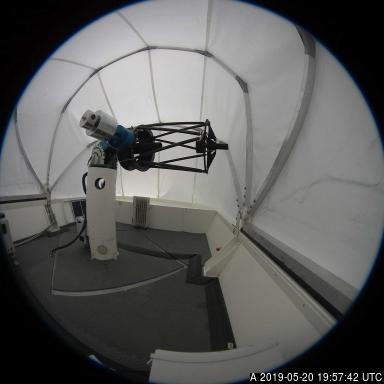
\includegraphics[height=0.6\linewidth]{figures/coatli-webcam-a.jpg}
\fi
\ifddotioan
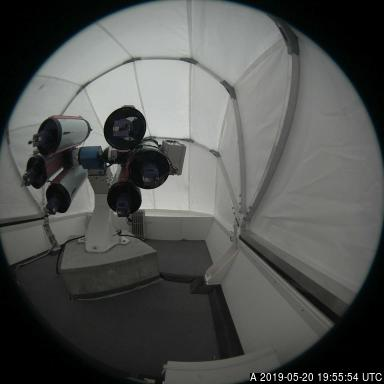
\includegraphics[height=0.6\linewidth]{figures/ddoti-webcam-a.jpg}
\fi
\end{center}
\caption{Typical daytime view from {\projectname} webcam A.}
\label{figure:webcam-a-view}
\begin{center}
\ifcoatlioan
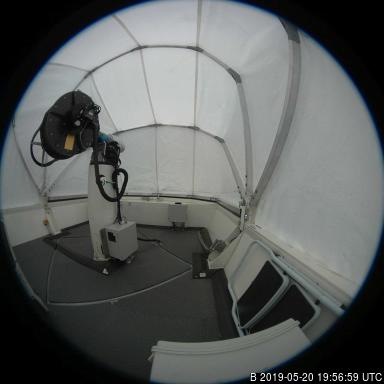
\includegraphics[height=0.6\linewidth]{figures/coatli-webcam-b.jpg}
\fi
\ifddotioan
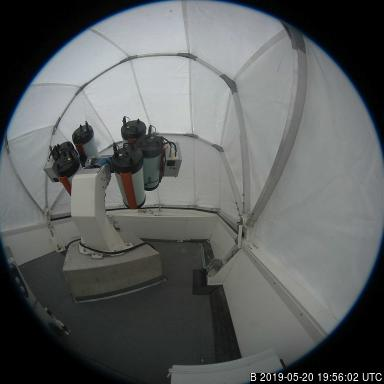
\includegraphics[height=0.6\linewidth]{figures/ddoti-webcam-b.jpg}
\fi
\end{center}
\caption{Typical daytime view from {\projectname} webcam B.}
\label{figure:webcam-b-view}
\end{figure}

\begin{figure}[t]
\begin{center}
\ifcoatlioan
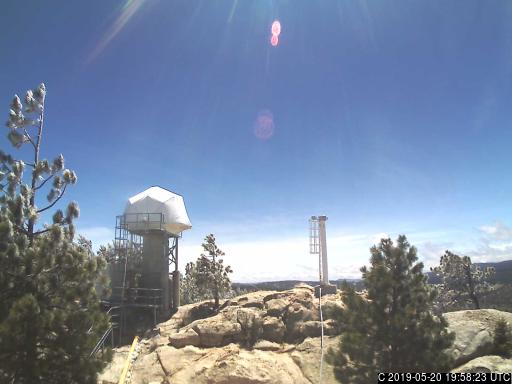
\includegraphics[height=0.6\linewidth]{figures/coatli-webcam-c.jpg}
\fi
\ifddotioan
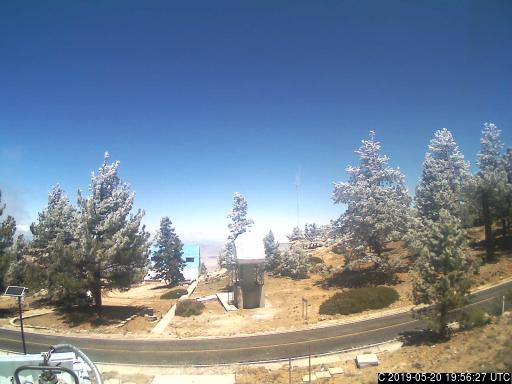
\includegraphics[height=0.6\linewidth]{figures/ddoti-webcam-c.jpg}
\fi
\end{center}
\caption{Typical daytime view from {\projectname} webcam C.}
\label{figure:webcam-c-view}
\begin{center}
\ifcoatlioan
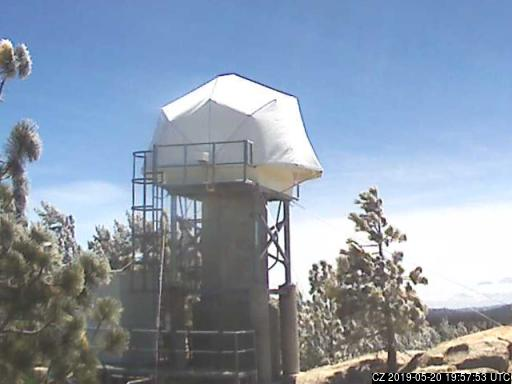
\includegraphics[height=0.6\linewidth]{figures/coatli-webcam-cz.jpg}
\fi
\ifddotioan
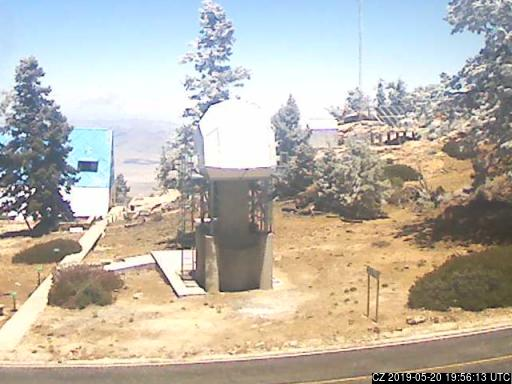
\includegraphics[height=0.6\linewidth]{figures/ddoti-webcam-cz.jpg}
\fi
\end{center}
\caption{Typical daytime view from {\projectname} webcam CZ (en electronic zoom of webcam C).}
\label{figure:webcam-cz-view}
\end{figure}

\section{Platform Webcams}

There are two webcams installed on short posts on the platform. Webcam A is installed above Box B and webcam B is installed above Box C. Figures~\ref{figure:webcam-a-view} and \ref{figure:webcam-b-view} show typical daytime views from webcams A and B. Between them, they can see all of the platform. The platform remote light allow the webcams to monitor the platform even at night. The webcams are Vivotek FE8174V with a 180 degree field of view. This model has an IP66-rated weatherproof housing and can operate down to $-40$~C.

The platform webcams are on the LAN at the addresses given in Table~\ref{table:network-addresses}. The web interfaces can be accessed with the “\projectaccount” account with password “\projectaccount”.

\section{External}

Webcam C is installed on the outside wall of the 84-cm, above the balcony, giving a view of the {\projectname} enclosure. An electronic zoom of webcam C, that shows the enclosure in more detail, is known as webcam CZ. Figures~\ref{figure:webcam-c-view} and \ref{figure:webcam-cz-view} show typical daytime views from webcams C and CZ.
The webcam is a Vivotek MD7560D with a $98 \times 73$ degree field of view lens. This model has an IP67-rated weatherproof housing and can operate down to $-25$~C.

The external webcam in on the observatory public network at the address given in Table~\ref{table:network-addresses}. The web interfaces can be accessed with the “\projectaccount” account with password “\projectaccount”.

\section{Bibliography}

\begin{flushleft}
\begin{itemize}
\item “\href{bibliography/vivotek-fe8174v-data-sheet.pdf}{FE8174/74V Data Sheet}”, Vivotek.
\item “\href{bibliography/vivotek-fe8174v-manual.pdf}{FE8174V User’s Manual}”, Vivotek.
\item “\href{bibliography/vivotek-md7560-alignment-sticker.pdf}{MD7530/60 MD8562/62D Alignment}”, Vivotek.
\item “\href{bibliography/vivotek-md7560-data-sheet.pdf}{MD7560/60D Data Sheet}”, Vivotek.
\item “\href{bibliography/vivotek-md7560-manual.pdf}{MD7530/7530D MD7560/7560D User’s Manual}”, Vivotek.
\item “\href{bibliography/vivotek-md7560-quick-instaltion-guide.pdf}{MD7530/7530D MD7560/7560D Quick Installation Guide}”, Vivotek.
\end{itemize}
\end{flushleft}

\chapter{Enclosure}
\label{chapter:enclosure}

\section{Description}

\begin{figure*}
\begin{center}
\ifcoatli
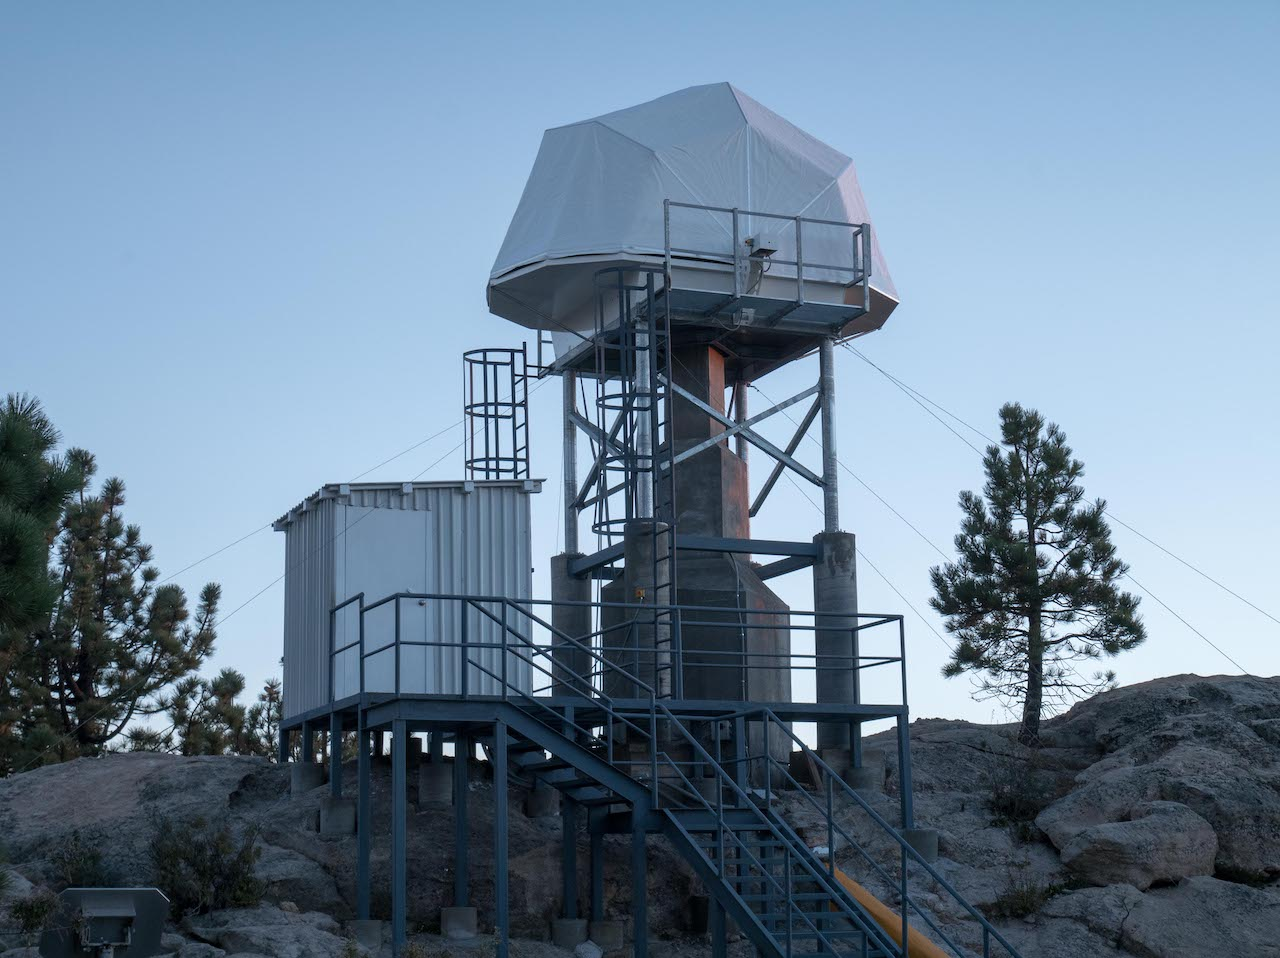
\includegraphics[width=0.8\linewidth]{figures/enclosure-coatli.jpg}
\fi
\ifddoti
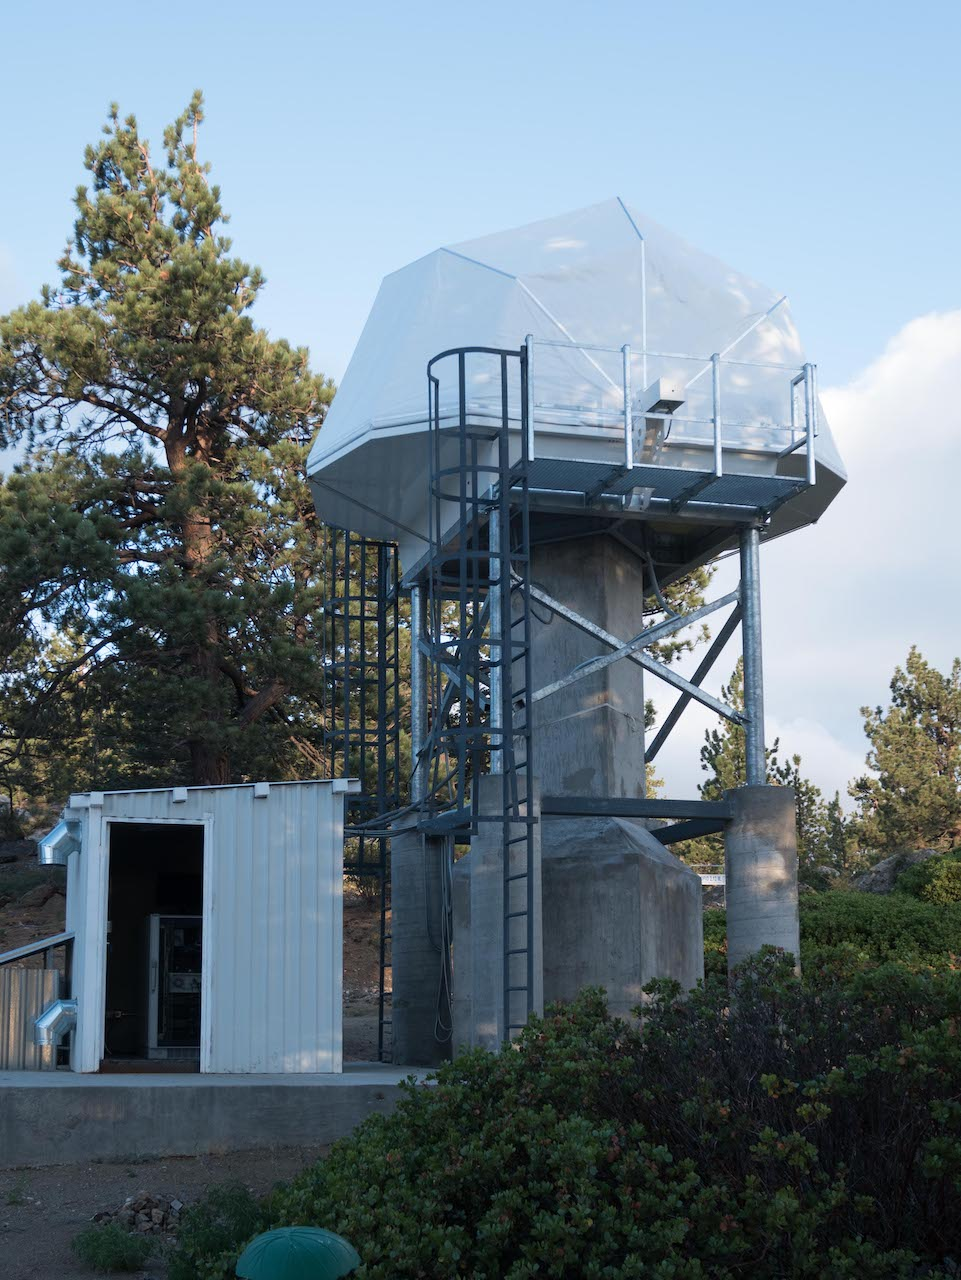
\includegraphics[width=0.8\linewidth]{figures/enclosure-ddoti.jpg}
\fi
\end{center}
\caption{The {\projectname} enclosure.}
\label{figure:enclosure}
\end{figure*}

{\projectname} is protected by an ASTELCO ARTS enclosure, shown in Figure~\ref{figure:enclosure}. The ARTS enclosure consists of a tower, a platform with balconies, and set of folding arches that support a flexible waterproof fabric roof. 

\safety{Under no circumstances ascend to the platform or balconies if the enclosure is in remote mode as the enclosure can close without warning.}

\ifcoatli
The enclosure can open to 60, 120, and 180 $\deg$ and can be controlled locally or remotely. The enclosure is oriented ENE to WSW and opens from the ENE towards the WSW.
\fi
\ifddoti
The enclosure can open to 60, 90, 120, and 180 $\deg$ and can be controlled locally or remotely. The enclosure is oriented NNE to SSW and opens from the NNE towards the SSW.
\fi


The enclosure can open and close in wind speeds of up to 90 km/h and has a survival windspeed of 180 km/h.

\begin{figure*}
\begin{center}
\ifcoatli
\includegraphics[width=0.6\linewidth]{figures/enclosure-coatli-controller.jpg}
\fi
\ifddoti
\includegraphics[width=0.6\linewidth]{figures/enclosure-ddoti-controller.jpg}
\fi
\end{center}
\caption{The enclosure controller in the shed.}
\label{figure:enclosure-controller}
\end{figure*}

The controller for the enclosure, shown in Figure~\ref{figure:enclosure-controller} is located in a cabinet in the shed. The enclosure is opened and closed by two geared motors, one on each balcony. The position is sensed by proximity sensors on the bearings (fully open and partially open positions) and at the point that the last arch closes (closed position). The controller and the motors are powered by 220 V 60 Hz from the Circuit A via the 220 V UPS and 220 V iBootBar.

\begin{figure*}
\begin{center}
\resizebox{\columnwidth}{!}{%
\begin{labeled}{\includegraphics[width=0.48\linewidth]{figures/enclosure-bearing-north.jpg}}
\arrowandlabel{(-0.9,-1.7)}{(-1.2,-4)}{north}{Emergency Button};
\arrowandlabel{(+0.3,-0.4)}{(+1.8,-4)}{north}{Allen Key};
\arrowandlabel{(+0.0,+2.1)}{(0,+4)}{south}{Proximity Sensors};
\end{labeled}
\space
\begin{labeled}{\includegraphics[width=0.48\linewidth]{figures/enclosure-bearing-south.jpg}}
\arrowandlabel{(0.2,+2.1)}{(0.2,+4)}{south}{Proximity Sensors};
\dummylabel{(-1.2,-4)}{north}
\end{labeled}}
\end{center}
\caption{The north (left) and south (right) bearings for the folding roof. Notice the proximity sensors, the emergency stop button for the mount, and the Allen key to escape in an emergency.
\ifddoti
The COATLI installation is shown, but the DDOTI installation is similar.
\fi
}
\label{figure:enclosure-bearing-north}
\label{figure:enclosure-beating-south}
\end{figure*}


\begin{figure*}
\begin{center}
\begin{labeled}{\includegraphics[width=0.8\linewidth]{figures/enclosure-electromagnetic-lock.jpg}}
\arrowandlabel{(-0.45,+0.7)}{(-0.45,+4)}{south}{Proximity Sensor}
\arrowandlabel{(-2.0,-2.0)}{(-2,-4)}{north}{Electromagnetic Lock};
\arrowandlabel{(+2.7,-1.2)}{(+2.7,-4)}{north}{Rain Sensor};
\end{labeled}
\end{center}
\caption{The enclosure electromagnetic lock (left), 0 $\deg$ proximity sensor (the cylinder with the blue top in the center), and rain sensor (the white box with the copper contacts on the right).
\ifddoti
The COATLI installation is shown, but the DDOTI installation is similar.
\fi
}
\label{figure:enclosure-electromagnetic-lock}
\end{figure*}

The enclosure has an electromagnetic lock, shown in Figure~\ref{figure:enclosure-electromagnetic-lock}, that holds it firmly closed. If the lock is not activated, the wind can open the roof a few centimeters and allow the ingress of rain or snow.

\safety{The enclosure controller should normally be switched on at all times in order to keep the electromagnetic lock activated.}

The electromagnet that holds the enclosure closed is normally activated by the PLC. However, we have modified the controller to add a switch inside the controller that switches on the enclosure electromagnet and actuates the enclosure emergency stop buttons. This ensures that the electromagnet stays energized even if the PLC fails and that the PLC cannot attempt to open the enclosure. This switch is shown in Figure~\ref{figure:enclosure-controller-manual-lock-switch}.

\begin{figure*}
\begin{center}
\ifcoatli
\resizebox{\columnwidth}{!}{%
\begin{labeled}{\includegraphics[width=\linewidth]{figures/enclosure-controller-inside-coatli.jpg}}
\arrowandlabel{(+1.75,-2.0)}{(+1.75,-6.5)}{north}{Manual Lock Switch};
\end{labeled}}
\fi
\ifddoti
\resizebox{\columnwidth}{!}{%
\begin{labeled}{\includegraphics[width=\linewidth]{figures/enclosure-controller-inside-ddoti.jpg}}
\arrowandlabel{(+1.5,-2.3)}{(+1.5,-6.5)}{north}{Manual Lock Switch};
\end{labeled}}
\fi
\end{center}
\caption{The inside of the enclosure controller cabinet showing the manual switch for the electromagnet.}
\label{figure:enclosure-controller-manual-lock-switch}
\end{figure*}

The enclosure has a rain sensor, also shown in Figure~\ref{figure:enclosure-electromagnetic-lock}. In automatic mode, it will automatically close if the rain sensor gets wet.

\begin{figure*}
\begin{center}
\begin{labeled}{\includegraphics[width=0.8\linewidth]{figures/enclosure-safety-seal.jpg}}
\arrowonly{(-0.2,+0.4)}{(-0.45,+4)}{south};
\arrowonly{(-3.0,-0.9)}{(-0.45,+4)}{south};
\arrowandlabel{(+3.0,+0.4)}{(-0.45,+4)}{south}{Safety Seal};
\end{labeled}
\end{center}
\caption{The enclosure safety seal, the black rubber seal on the lower edge of the enclosure opening. If this is pressed, the motors will stop and an error is set in the controller.
\ifddoti
The COATLI installation is shown, but the DDOTI installation is similar.
\fi
}
\label{figure:enclosure-safety-seal}
\end{figure*}

The enclosure has a safety seal along the lower edge of the opening. The motors will stop if this is pressed. This avoids the enclosure closing on someone or something. However, it is easy to activate the safety rail when entering or leaving the enclosure. 

\begin{figure*}
\begin{center}
\resizebox{\columnwidth}{!}{%
\begin{labeled}{\includegraphics[width=0.48\linewidth]{figures/enclosure-emergency-stop-lower.jpg}}
\arrowandlabel{(-0.7,+0.8)}{(-0.7,+2.5)}{south}{Emergency Button};
\end{labeled}
\space
\begin{labeled}{\includegraphics[width=0.48\linewidth]{figures/enclosure-emergency-stop-upper.jpg}}
\arrowandlabel{(-0.0,+0.4)}{(-0.0,+2.5)}{south}{Emergency Button};
\end{labeled}}
\end{center}
\caption{The enclosure emergency stop buttons, next to the main access ladder (left) and on the northern motor cowling (right).
\ifddoti
The COATLI installation is shown, but the DDOTI installation is similar.
\fi
}
\label{figure:enclosure-emergency-stop}
\end{figure*}

The enclosure also has two emergency stop buttons, one at the bottom of the main access ladder and the other on the northern motor cowling. These are shown in Figure~\ref{figure:enclosure-emergency-stop}. Again, the motors will stop if either of these are pressed.

\begin{figure*}
\begin{center}
\resizebox{\columnwidth}{!}{%
\includegraphics[width=0.48\linewidth]{figures/enclosure-elevated-east.jpg}%
\space
\includegraphics[width=0.48\linewidth]{figures/enclosure-elevated-west.jpg}%
}
\end{center}
\caption{Do not walk on the elevated areas at the ends of the platform as they are not load bearing. Note the “no step” signs.
\ifddoti
The COATLI installation is shown, but the DDOTI installation is similar.
\fi
}
\label{figure:enclosure-elevated}
\end{figure*}

The two semi-circular elevated areas at the ends of the platform, shown in Figure~\ref{figure:enclosure-elevated}, are not load bearing and are marked with “no step” signs. If you attempt to walk on these, you will likely fall.

\safety{Do not walk on the elevated areas at the ends of the platform!}

If you are trapped in the enclosure and cannot summon help, you can escape by using the Allen key taped below the northern bearing to remove one of the sloping side panels to gain access to the balcony. See Figure~\ref{figure:enclosure-bearing-north}.

\begin{figure*}
\begin{center}
\ifcoatli
\resizebox{\linewidth}{!}{\begin{labeled}{\includegraphics[width=\linewidth]{figures/enclosure-coatli-controller-door.jpg}}
%\draw[dotted] (-5,-5) grid (+5,+5);
\arrowandlabel{(-1.1,-0.6)}{(-4.0,-6.4)}{north}{Mode Selector Switch};
\arrowandlabel{(+1.1,-0.6)}{(+4.0,-6.4)}{north}{Angle Selector Switch};
\arrowandlabel{(+0.0,-4.0)}{(+0.0,-6.4)}{north}{Main Power Switch};
\arrowandlabel{(-2.1,+3.5)}{(-3.0,+6.4)}{south}{Open Button};
\arrowandlabel{(+2.2,+3.5)}{(+3.0,+6.4)}{south}{Close Button};
\arrowandlabel{(+0.0,+3.5)}{(+0.0,+6.4)}{south}{Error Button};
\end{labeled}}
\fi
\ifddoti
\resizebox{\linewidth}{!}{\begin{labeled}{\includegraphics[width=\linewidth]{figures/enclosure-ddoti-controller-door.jpg}}
%\draw[dotted] (-5,-5) grid (+5,+5);
\arrowandlabel{(-1.1,-0.6)}{(-4.0,-6.4)}{north}{Mode Selector Switch};
\arrowandlabel{(+1.1,-0.6)}{(+4.0,-6.4)}{north}{Angle Selector Switch};
\arrowandlabel{(+0.0,-4.0)}{(+0.0,-6.4)}{north}{Main Power Switch};
\arrowandlabel{(-2.1,+3.5)}{(-3.0,+6.4)}{south}{Open Button};
\arrowandlabel{(+2.2,+3.5)}{(+3.0,+6.4)}{south}{Close Button};
\arrowandlabel{(+0.0,+3.5)}{(+0.0,+6.4)}{south}{Error Button};
\end{labeled}}
\fi
\end{center}
\caption{The enclosure controller door and control panel. Bottom: the main power switch. Middle row, left to right: the mode selector switch (“LOCAL” and “REMOTE”) and the angle selector switch (180 $\deg$ is fully open). Top row, left to right: the open button, the error button, and the close button.
}
\label{figure:enclosure-controller-door}
\end{figure*}

The enclosure controller can be in remote or local mode. The mode is selected by the switch on the door of the enclosure controller in the shed (see Figure~\ref{figure:enclosure-controller-door}). In remote mode:
\begin{itemize}
\item
The switches on the enclosure controller to open and close the enclosure and to reset errors are deactivated.
\item
The robotic control system can open and close. 
\item
The enclosure will close automatically if the rain sensor gets wet.
\end{itemize}
In local mode:
\begin{itemize}
\item
The switches on the enclosure controller to open and close the enclosure and to reset errors are active.
\item
The robotic control system cannot open or close. 
\item
The enclosure will not close if the rain sensor gets wet.
\end{itemize}

If there is an error, the red error button on the enclosure controller will flash or be constantly lit. The interpretation depends on whether the controller is in local mode or remote more.

In remote mode, the red button will be constantly illuminated for all detected errors. The specific error can be diagnosed either by software (via the inputs to the ADAM module) or by switching to local mode.

In local mode, the following error states are distinguished:

\begin{itemize}
\item Constant: One or both of the emergency stop buttons have been pressed. There is one emergency stop button at the bottom of the north ladder and another on the cowling around the north motor. Follow the procedure in \S\ref{section:enclosure:reset-emergency-button} to clear the error.
\item Slow flashing (1 Hz): The motor under-current relay (K6) has been activated.
\item Medium flashing (2 Hz): One or both of the motor over-current relays (K7 and K8) have been activated. This can happen if the enclosure is opened and closed continously for several minutes. Follow the procedure in \S\ref{section:enclosure:reset-motot-over-current} to clear the error.
\item Fast flashing (4 Hz): The safety seal around the enclosure cover has been activated. Follow the procedure in \S\ref{section:enclosure:reset-safety-seal} to clear the error.
\end{itemize}

\section{Maintenance Procedures}

\subsection{Enabling Remote Mode}
\label{section:enclosure-enabling-remote-mode}

\subsubsection{Safety Considerations}

\safety{Under no circumstances ascend to the platform or balconies if the enclosure is in remote mode as the enclosure can close without warning.}

\subsubsection{Requirements}

You will need:

\begin{itemize}
\item One person.
\item The key to the shed (see \S\ref{section:shed-key}).
\end{itemize}

\subsubsection{Procedure}


\begin{enumerate}
\item
Go to the shed.
\item
Move the main power switch on the enclosure controller door to “ON”.
\item
Move the mode selector switch on the enclosure controller door to “REMOTE”.
\end{enumerate}

\subsection{Opening or Closing in Local Mode}
\label{section:enclosure-opening-or-closing-in-local-mode}

\subsubsection{Safety Considerations}

\safety{In local mode, the control system cannot open or close enclosure.}

\safety{In local mode, the rain sensor cannot close enclosure.}

\safety{Before opening the enclosure, check on the webcams that the telescope is not pointed to towards the sun. In the home position, the telescope is pointed to the north pole.}

\subsubsection{Requirements}

You will need:

\begin{itemize}
\item One person (to open or close only) or two or more persons (if you wish to ascend to the platform).
\item The key to the shed (see \S\ref{section:shed-key}).
\end{itemize}

\subsubsection{Procedure}

\begin{enumerate}
\item
Go to the shed.
\item
Move the enclosure controller main power switch on the enclosure controller to “ON”.
\item
Move the enclosure controller mode selector switch to “LOCAL”.
\item
If there is an error, the red error button will flash or be constantly lit. Investigate the error, and clear it before proceeding:

In local mode, the following error states are distinguished:

\begin{itemize}
\item Constant: One or both of the emergency stop buttons have been pressed. There is one emergency stop button at the bottom of the north ladder and another on the cowling around the north motor. Follow the procedure in \S\ref{section:enclosure:reset-emergency-button} to clear the error.
\item Slow flashing (1 Hz): The motor under-current relay (K6) has been activated.
\item Medium flashing (2 Hz): One or both of the motor over-current relays (K7 and K8) have been activated. This can happen if the enclosure is opened and closed continously for several minutes. Follow the procedure in \S\ref{section:enclosure:reset-motot-over-current} to clear the error.
\item Fast flashing (4 Hz): The safety seal around the enclosure cover has been activated. Follow the procedure in \S\ref{section:enclosure:reset-safety-seal} to clear the error.
\end{itemize}

\item
To open, set the angle selector switch to the desired angle (60, 120, and 180 $\deg$) and then press and hold the open button until the green light goes out. The 60 $\deg$ position gives access to the dome while continuing the shade the telescope from the elements.
\item
To close, press and hold the green close button until the light goes out.
\item
If you wish to subsequently operate the enclosure remotely, move the mode selector switch to “REMOTE”.
\end{enumerate}

\subsection{Resetting a Safety Seal Error}
\label{section:enclosure:reset-safety-seal}

If the safety seal is pressed the error button on the enclosure controller door flashes at 4 Hz in local mode and the enclosure will not operate. This procedure describes how to reset the error.

\subsubsection{Safety Considerations}

\safety{Use a harness, line, and helmet when you work on the platform or balconies.}

\subsubsection{Requirements}

You will need:
\begin{itemize}
\item At least two persons.
\item The key to the shed (see \S\ref{section:shed-key}).
\end{itemize}

\subsubsection{Procedure}

\begin{enumerate}
\item 
Go to the shed.
\item
Move the enclosure controller main power switch on the enclosure controller to “ON”.
\item
Move the enclosure controller mode selector switch to “LOCAL”.
\item
One person should use a safety harness, safety line, and safety helmet and ascend to the platform. They should remove whatever is pressing the safety seal. They should then descend from the platform.
\item
Press the error button to clear the error.
\item
Attempt to move the enclosure slightly using the open or close buttons.
\item
Verify that the error button no longer signals an error. That is, that is no longer flashes. If not, continue to investigate the error.
\item
Close the enclosure.
\item
If you wish to subsequently operate the enclosure remotely, move the mode selector switch to “REMOTE”.
\end{enumerate}

\subsection{Resetting a Motor Over-Current Error}
\label{section:enclosure:reset-motot-over-current}

The motors are protected by over-current relays. In normal operation, these should not activate. However, if they do the error button on the enclosure controller door flashes at 2 Hz in local mode and the enclosure will not operate. This procedure describes how to reset the error.

\subsubsection{Safety Considerations}

\safety{Be extremely careful when working inside the controller cabinet as it uses 220 VAC.}

\subsubsection{Requirements}

You will need:
\begin{itemize}
\item One person.
\item The key to the shed (see \S\ref{section:shed-key}).
\end{itemize}

\subsubsection{Procedure}

\begin{enumerate}
\item
Go to the shed.
\item
Move the mode selector switch to “LOCAL”.
\item
Move the enclosure controller main power switch on the enclosure controller to “OFF”.
\item
Open the enclosure controller door.
\item
Locate the motor over-current relays K7 and K8 (see Figure~\ref{figure:enclosure-controller-inside}). Press the blue buttons on K7 and K8 to reset them.
\item
Close the enclosure controller door.
\item
Move the enclosure controller main power switch on the enclosure controller to “ON”.
\item
Attempt to move the enclosure slightly using the open or close buttons.
\item
Verify that the error button no longer signals an error. That is, that is no longer flashes. If not, continue to investigate the error.
\item
Close the enclosure.
\item
If you wish to subsequently operate the enclosure remotely, move the mode selector switch to “REMOTE”.
\end{enumerate}

\subsection{Resetting an Emergency Button Error}
\label{section:enclosure:reset-emergency-button}

If one of the emergency buttons is pressed the error button on the enclosure controller door will be constantly lit in local mode and the enclosure will not operate. This procedure describes how to reset the error.

\subsubsection{Safety Considerations}

\safety{Use a harness, line, and helmet when you work on the platform or balconies.}

\subsubsection{Requirements}

You will need:
\begin{itemize}
\item At least two people.
\item The key to the shed (see \S\ref{section:shed-key}).
\end{itemize}

\subsubsection{Procedure}

\begin{enumerate}
\item 
Check the emergency button at the bottom of the ladder. If it is activated, twist it clockwise to release it.
\item
One person should use a safety harness, safety line, and safety helmet and ascend to the platform. They should check the emergency button at on the north motor casing. If it is activated, they should twist it clockwise to release it. They should then descend from the platform.
\item
Move the mode selector switch to “LOCAL”.
\item
Press the error button to clear the error.
\item
Attempt to move the enclosure slightly using the open or close buttons.
\item
Verify that the error button no longer signals an error. That is, that is no longer flashes. If not, continue to investigate the error.
\item
Close the enclosure.
\item
If you wish to subsequently operate the enclosure remotely, move the mode selector switch to “REMOTE”.
\end{enumerate}

%\subsection{Manual Opening or Closing with Power}
%\label{section:enclosure-manual-opening-or-closing-with-power}
%
%If the enclosure cannot be operated normally using remote mode or local mode, you can bypass the control system and operate it manually. There are two modes, depending on whether power is available. Here we document the procedure for opening or closing with power. In \S\ref{section:enclosure-manual-opening-or-closing-without-power} we document the procedure for opening or closing without power.
%
%\begin{figure*}
%\begin{center}
%\includegraphics[width=0.7\linewidth]{figures/enclosure-controller-plc-disconnected.jpg}
%\end{center}
%\caption{The PLC U2 is deactivated by removing the two cables from the L+ terminal of U2.}
%\label{figure:enclosure-controller-plc-deactivated}
%\bigskip
%\begin{center}
%\includegraphics[width=0.7\linewidth]{figures/enclosure-controller-jumpers.jpg}
%\end{center}
%\caption{Jumpers shorting the PLC relays. The yellow jumper shorting Q1 of U3 deactivates the motor breaks. The green jumper shorting Q1 of U4 activates the electromagnetic lock.}
%\label{figure:enclosure-controller-jumpers}
%\end{figure*}
%
%\begin{figure*}
%\begin{center}
%\includegraphics[width=0.7\linewidth]{figures/enclosure-controller-k6-activated.jpg}
%\end{center}
%\caption{The green LED on K6 lights up indicates that the motor brakes have been deactivated. The orange LED to the right of the green LED also lights up for a few seconds.}
%\label{figure:enclosure-controller-k6-activated}
%\bigskip
%\begin{center}
%\includegraphics[width=0.8\linewidth]{figures/enclosure-controller-relays.jpg}
%\end{center}
%\caption{The relays that control the motors (K1 and K4 to close and K2 and K3 to open) and motor brakes (K5).}
%\label{figure:enclosure-controller-relays}
%\end{figure*}
%
%\begin{figure*}
%\begin{center}
%\includegraphics[width=0.7\linewidth]{figures/enclosure-controller-diode.jpg}
%\end{center}
%\caption{The diode across terminals 24 and 25 of the output connector. When the electromagnetic lock is activated, there are 24 VDC across the diode.}
%\label{figure:enclosure-controller-diode}
%\end{figure*}
%
%If power is available and the motors work, the enclosure can be opened and closed by manually activating the relays in the enclosure controller for the motor brakes, motors, and electromagnetic lock.
%
%This is not to be undertaken lightly, as there are risks both to personnel and equipment. First, these procedures require working in proximity to live 220 VAC. Second, many of the usual safety features that protect the equipment are not available. For example, if you accidentally activate the motor relays incorrectly, you can short the relays and will probably damage them.  For a similar reason, it is necessary to disable the PLC to avoid it attempting to activate the relays while they are being activated manually.
%
%\subsubsection{Safety Considerations}
%
%\safety{Be extremely careful when working inside the controller cabinet as it uses 220 VAC.}
%
%\subsubsection{Requirements}
%
%You will need:
%\begin{itemize}
%\item At least one person.
%\item Two small flat-headed screwdrivers.
%\item Two low-voltage jumper cables.
%\item A multimeter.
%\item The key to the shed (see \S\ref{section:shed-key}).
%\end{itemize}
%All of these can be found in the tool box in the {\projectname} equipment cabinet in the ground floor of the 84-cm telescope building.
%
%\subsubsection{Procedure for Closing the Enclosure}
%
%To close the enclosure:
%
%\begin{enumerate}
%\item
%Go to the shed.
%
%\item Switch off the enclosure controller.
%
%Move the main power switch on the controller door from ON to OFF.
%
%\item Deactivate the PLC.
%
%Remove the two cables from the L+ terminal of U2. See Figure~\ref{figure:enclosure-controller-plc-deactivated}.
%
%\item Prepare to deactivate the motor brakes.
%
%Short the Q1 relay of U3 using a jumper cable. See Figure~\ref{figure:enclosure-controller-jumpers}.
%
%\item Prepare to activate the electromagnetic lock.
%
%Short the Q1 relay of U4 using a jumper cable. See Figure~\ref{figure:enclosure-controller-jumpers}.
%
%\item Switch on the enclosure controller.
%
%Move the main power switch on the controller door from OFF to ON.
%
%\item 
%Check that the PLC is deactivated. 
%
%Check that the RUN/STOP LED on U2 does not light up. See Figure~\ref{figure:enclosure-controller-plc-deactivated}. (The RUN/STOP LEDs on U3 and U4 should light up.) If the LED on U2 does light up, you have not correctly disconnected its power. Start again.
%
%\item 
%Check that the motor breaks are deactivated. 
%
%Check that the green LED on K6 lights up to indicate that the motor brakes have been deactivated. The orange LED to the right of the green LED should also lights up for a few seconds. See Figure~\ref{figure:enclosure-controller-k6-activated}. If they do not do this, you have not correctly connected the jumper across the Q1 relay of U3. Start again.
%
%\item
%Check that the electromagnetic lock is activated. 
%
%Check that there is 24 VDC across the diode between terminal 24 and 25 of the output connector. See Figure~\ref{figure:enclosure-controller-diode}. If there is not, you have not correctly connected the jumper across the Q1 relay of U4. Start again.
%
%\item Run the motors to close the enclosure. 
%
%Use two screwdrivers to move the sliders of K1 and K4 from 0 to 1 and hold them there until the enclosure is closed. See Figure~\ref{figure:enclosure-controller-relays}. You may stop opening the enclosure at any point by releasing the sliders. Once the enclosure is fully closed you will hear the relays K9 and K10 activating and you should release the sliders. 
%
%\item Switch off the enclosure controller.
%
%Move the main power switch on the controller door from ON to OFF.
%
%\item Prepare to activate the motor brakes.
%
%Remove the jumper shorting Q1 of U3.
%
%\item Switch on the enclosure controller.
%
%Move the main power switch on the controller door from OFF to ON.
%
%\end{enumerate}
%
%\subsubsection{Procedure for Opening the Enclosure}
%
%To open the enclosure:
%
%\begin{enumerate}
%\item Switch off the enclosure controller.
%
%Move the main power switch on the controller door from ON to OFF.
%
%\item Deactivate the PLC.
%
%Remove the two cables from the L+ terminal of U2. See Figure~\ref{figure:enclosure-controller-plc-deactivated}.
%
%\item Prepare to deactivate the motor brakes.
%
%Short the Q1 relay of U3 using a jumper cable. See Figure~\ref{figure:enclosure-controller-jumpers}.
%
%\item Prepare to deactivate the electromagnetic lock.
%
%If you have previously activated the electromagnetic lock by shorting the Q1 relay of U4 using a jumper cable, remove the jumper cable. See Figure~\ref{figure:enclosure-controller-jumpers}.
%
%\item Switch on the enclosure controller.
%
%Move the main power switch on the controller door from OFF to ON.
%
%\item 
%Check that the PLC is deactivated. 
%
%Check that the RUN/STOP LED on U2 does not light up. See Figure~\ref{figure:enclosure-controller-plc-deactivated}. (The RUN/STOP LEDs on U3 and U4 should light up.) If the LED on U2 does light up, you have not correctly disconnected its power. Start again.
%
%\item 
%Check that the motor breaks are deactivated. 
%
%Check that the green LED on K6 lights up to indicate that the motor brakes have been deactivated. The orange LED to the right of the green LED should also lights up for a few seconds. See Figure~\ref{figure:enclosure-controller-k6-activated}. If they do not do this, you have not correctly connected the jumper across the Q1 relay of U3. Start again.
%
%\item
%Check that the electromagnetic lock is deactivated. 
%
%Check that there is 0 VDC across the diode between terminal 24 and 25 of the output connector. See Figure~\ref{figure:enclosure-controller-diode}. If there is not, you have not correctly disconnected the jumper across the Q1 relay of U4. Start again.
%
%\item Run the motors to open the enclosure. 
%
%Use two screwdrivers to move the sliders of K2 and K3 from 0 to 1 and hold them there until the enclosure is open. See Figure~\ref{figure:enclosure-controller-relays}. You may stop opening the enclosure at any point by releasing the sliders. Once the enclosure is fully open you will hear the relays K9 and K10 activating and you should release the sliders. 
%
%\item Switch off the enclosure controller.
%
%Move the main power switch on the controller door from ON to OFF.
%
%\item Prepare to activate the motor brakes.
%
%Remove the jumper shorting Q1 of U3.
%
%\item Switch on the enclosure controller.
%
%Move the main power switch on the controller door from OFF to ON.
%
%\end{enumerate}

\subsection{Manual Opening or Closing without Power}
\label{section:enclosure-manual-opening-or-closing-without-power}

If the enclosure cannot be operated normally using remote mode or local mode, you can bypass the control system and operate it manually by driving the motor axles manually with portable electric drills. This procedure requires two people. 

%There are two modes, depending on whether power is available. Here we document the procedure for opening or closing without power. In \S\ref{section:enclosure-manual-opening-or-closing-with-power} we documented the procedure for opening or closing with power.

This is not to be undertaken lightly, as it involves working on the balcony. However, when carried out with appropriate safety precautions and with calm, it is quite safe.

\subsubsection{Safety Considerations}

\safety{Be extremely careful when working inside the controller cabinet as it uses 220 VAC.}

\safety{Use a harness, line, and helmet when you work on the platform or balconies.}

\subsubsection{Requirements}

You will need:

\begin{itemize}
\item Two people.
\item Two portable electrical drills with 6 mm hex drives.
\item The key to the shed (see \S\ref{section:shed-key}).
\end{itemize}

Two suitable drills with drives are stored in the {\projectname} equipment cabinet in the ground floor of the 84-cm telescope building. The batteries are normally connected to wall socket.

\subsubsection{Procedure for Closing the Enclosure}


\begin{figure*}
\begin{center}
\includegraphics[width=0.7\linewidth]{figures/enclosure-closing-with-drills.jpg}
\end{center}
\caption{Opening or closing the enclosure with portable electric drills. The motor brake is disengaged by pushing the lever under the motor away from the platform.}
\label{figure:enclosure-closing-with-drills}
\end{figure*}

To close the enclosure:

\begin{enumerate}
\item Switch off the enclosure controller.

Move the main power switch on the controller door from ON to OFF.

%\item Deactivate the PLC.
%
%Remove the two cables from the L+ terminal of U2. See %Figure~\ref{figure:enclosure-controller-plc-deactivated}.

%\item Prepare to activate the electromagnetic lock.
%
%Short the Q1 relay of U4 using a jumper cable. See Figure~\ref{figure:enclosure-controller-jumpers}.

%\item Switch on the enclosure controller.
%
%Move the main power switch on the controller door from OFF to ON.

%\item 
%Check that the PLC is deactivated. 
%
%Check that the RUN/STOP LED on U2 does not light up. See Figure~\ref{figure:enclosure-controller-plc-deactivated}. (The RUN/STOP LEDs on U3 and U4 should light up.) If the LED on U2 does light up, you have not correctly disconnected its power. Start again.

%\item
%Check that the electromagnetic lock is activated. 
%
%Check that there is 24 VDC across the diode between terminal 24 and 25 of the output connector. See Figure~\ref{figure:enclosure-controller-diode}. If there is not, you have not correctly connected the jumper aross the Q1 relay of U4. Start again.


\item
Use appropriate safety equipment: harnesses, lines, and helmets. These are found in the shed.

\item
One person should ascend to one balcony with one drill and the other person to the other balcony with the other drill.

\item
Use your safety line to secure yourself to the balcony rail. Loop the line over the rail and then fasten the clasp on the line itself.

\item
Set the direction of the drill appropriately to close the enclosure.

\item
Insert the drill into the motor axle. See Figure~\ref{figure:enclosure-closing-with-drills}.

\item
Push the lever underneath the motor away from the platform to release the brake. Keep the brake released and run the electric drill to turn the motor axle. The two people should do this relatively slowly and coordinate; if one gets too far ahead of or behind the other, you can damage the arch or bearing.

\item
Once the enclosure is closed, release the brake lever, remove the drills, and descend from the platform.

\item
Open the enclosure controller.

\item
Engage the manual lock. This switches on the enclosure electromagnet and actuates the enclosure emergency stop buttons. This ensures that the electromagnet stays energized even if the PLC fails and that the PLC cannot attempt to open the enclosure.

Move the manual lock switch inside the enclosure controller from OFF to ON. See Figure~\ref{figure:enclosure-controller-manual-lock-switch}.

\item
Close the enclosure controller.

\item
Switch on the enclosure controller.

Move the main power switch on the controller door from OFF to ON.

\item
Place the enclosure in remote mode.

Move the enclosure controller mode selector switch to “REMOTE”.

\end{enumerate}

\subsubsection{Procedure for Opening the Enclosure}

To open the enclosure:

\begin{enumerate}
\item Switch off the enclosure controller.

Move the main power switch on the controller door from ON to OFF.

\item
Open the enclosure controller.

\item
Disengage the manual lock.

Move the manual lock switch inside the enclosure controller from ON to OFF. See Figure~\ref{figure:enclosure-controller-manual-lock-switch}.

\item
Close the enclosure controller.

\item
Use appropriate safety equipment: harnesses, lines, and helmets. These are found in the shed.

\item
One person should ascend to the northern balcony with one drill and one to the southern balcony with the other drill.

\item
Use your safety line to secure yourself to the balcony rail. Loop the line over the rail and then fasten the clasp on the line itself.

\item
Set the direction of the drill appropriately to open the enclosure.

\item
Insert the drill into the motor axle. See Figure~\ref{figure:enclosure-closing-with-drills}.

\item
Push the lever underneath the motor away from the platform to release the brake. Keep the brake released and run the electric drill to turn the motor axle. The two people should do this relatively slowly and coordinate; if one gets too far ahead of or behind the other, you can damage the arch or bearing.

\item
Once the enclosure is open, release the brake lever, remove the drills, and descend from the platform.

\item
Switch on the enclosure controller.

Move the main power switch on the controller door from OFF to ON.

\end{enumerate}

\subsection{Shutting-Down Before and Starting-Up After the Winter Break}
\label{section:enclosure-manual-winter-break}

The observatory and {\projectname} cease operations during a winter break of about three weeks. During the winter break the enclosure should be left closed and powered on but with a hardware override on the electromagnetic lock.

\subsubsection{Safety Considerations}

\safety{Be extremely careful when working inside the controller cabinet as it uses 220 VAC.}

\subsubsection{Requirements}

You will need:
\begin{itemize}
\item At least one person.
\item The key to the shed (see \S\ref{section:shed-key}).
\end{itemize}
All of these can be found in the tool box in the {\projectname} equipment cabinet in the ground floor of the 84-cm telescope building.

\subsubsection{Procedure for Shutting-Down Before the Winter Break}

To prepare the enclosure before the winter break:

\begin{enumerate}
\item
Go to the shed.

\item
Move the enclosure controller mode selector switch to “LOCAL”.

\item If the weather permits, open the enclosure to 60 $\deg$.

Set the angle selector switch to the 60 $\deg$ and then press and hold the open button until the green light goes out.

\item Close the dome.

Press and hold the close button until the green light goes out.

\item Switch off the enclosure controller.

Move the main power switch on the controller door from ON to OFF.

\item
Open the enclosure controller.

\item
Engage the manual lock. This switches on the enclosure electromagnet and actuates the enclosure emergency stop buttons. This ensures that the electromagnet stays energized even if the PLC fails and that the PLC cannot attempt to open the enclosure.

Move the manual lock switch inside the enclosure controller from OFF to ON. See Figure~\ref{figure:enclosure-controller-manual-lock-switch}.

\item
Close the enclosure controller.

\item Leave the enclosure controller mode selector switch to “LOCAL”.

\end{enumerate}

\subsubsection{Procedure for Starting-Up After the Winter Break}

To prepare the enclosure after the winter break:

\begin{enumerate}
\item
Go to the shed.

\item Switch off the enclosure controller.

Move the main power switch on the controller door from ON to OFF.

\item Open the enclosure controller.

\item
Disengage the manual lock.

Move the manual lock switch inside the enclosure controller from ON to OFF. See Figure~\ref{figure:enclosure-controller-manual-lock-switch}.

\item
Close the enclosure controller.

\item Switch on the enclosure controller.

Move the main power switch on the controller door from OFF to ON.

\item Move the enclosure controller mode selector switch to “REMOTE”.

\end{enumerate}

\section{Remote Interface}

\subsection{Lantronix EDS}

The RS-232 interface to the enclosure controller is made available via the Lantronix EDS 4100 ethernet-to-serial converter. Specifically, it is connected to line 3 and configured as 9600/8-N-1 with a tunnel on TCP port 10003.

The Lantronix EDS is on the LAN at \verb|serial|.

\subsection{ADAM Modules}
\label{section:enclosure-adam-modules}

Remote control of the enclosure is through an ADAM-4055 digital input/output module. The input and output channels of the ADAM-4055 module are connected to the enclosure controller PLC.

The RS-485 serial interface of the ADAM-4055 is exposed via an ADAM-4520 RS-232 to RS-485 converter and isolator as RS-232 at 9600/8-N-1.

The state of the input and output channels can be determined either from the web interface (the “Input Channels” and “Output Channels” variables in the “Enclosure” tab) or by unscrewing the ADAM-4520 RS-232 to RS-485 converter on top of the ADAM-4055 to reveal LEDs which show the state of the channels.

The input channels are:
\begin{description}
\item[DI0] Open. 0 = not open and 1 = open. This channel is connected to terminal U3/Q5 (“Kuppel AUF”) on the PLC. Its value is determined by the PLC from the proximity switches on the platform.
\item[DI1] Closed. 0 = not closed and 1 = closed. This channel is connected to terminal U3/Q6 (“Kuppel ZU”) on the PLC. Its value is determined by the PLC from the proximity switches on the platform.
\item[DI2] Error. In remote mode, 1 = error and 0 = no error. In local mode, this follows the state of the red error button (constant 0 = not error, constant 1 = emergency stop button pressed, and intermittent at 1, 2, or 4 Hz for under-current, over-current, and safety rail errors). This channel is connected to U3/Q4 (“Störung”) on the PLC, which also control the red error button. Its value is determined by the PLC. Note that the behavior of this channel in local mode makes it only useful in remote mode.
\item[DI3] Mode. 0 = local and 1 = remote. This channel is connected to terminal U4/I2 (“Hand/Auto”) of the PLC. Its value is directly determined by the mode switch. 
\item[DI4] Motor over-current error. 0 = no error and 1 = error. This channel is connected to terminal U3/I7 (“Motorschutz”) of the PLC. Its value is directly determined by the motor over-current relays K7 and K8.
\item[DI5] Rain sensor. 0 = dry and 1 = wet. This channel is connected to terminal U3/Q8 (“Regensensor”) on the PLC. Its value is determined by the PLC from the rain sensor switch on the platform. 
\item[DI6] Safety strip. 0 = not pressed and 1 = pressed. This channel is connected to terminal U4/I1 (“Dichtlippe”) on the PLC. Its value is directly determined by the safety rail switch.
\item[DI7] Emergency stop. 0 = not pressed and 1 = pressed. This channel is not connected to the PLC but rather to the emergency stop button circuit. Its value is determined directly by the emergency stop buttons.
\end{description}

The output channels are:
\begin{description}
\item[DO0] Open. In remote mode, set to 1 to open to the position specified by DO3, DO4, and DO5. This channel is connected to terminal U2/I3 (“AUF”) of the PLC via relay K11.
\item[DO1] Close. In remote mode, set to 1 to close. This channel is connected to terminal U2/I4 (“ZU”) of the PLC via relay K12.
\item[DO2] Reset. In remote mode, set to 1 to reset an error. This channel is connected to terminal U2/I8 (“Reset”) of the PLC via relay K13.
\item[DO3] 60 deg. Set to 1 to select 60 degrees. This channel is connected to terminal U4/I5 (“Auto 60-Grad”) of the PLC via relay K14.
\item[DO4] 90 deg. Set to 1 to select 90 degrees. This channel is connected to terminal U4/I6 (“Auto 90-Grad”) of the PLC via relay K15. 
\ifcoatli
(The {\projectname} enclosure does not have hardware to open to 90 degrees.)
\fi
\item[DO5] 120 deg. Set to 1 to select 120 degrees. This channel is connected to terminal U4/I7 (“Auto 120-Grad”) of the PLC via relay K16.
\item[DO6] Not used.
\item[DO7] Not used.
\end{description}

If D03, D04, and D05 are all set to 0, opening will open to 180 degrees. 
\ifcoatli
The {\projectname} enclosure has hardware to support opening to 60, 120, and 180 degrees; it does not have hardware to support opening to 90 degrees. 
\fi
\ifddoti
The {\projectname} enclosure has hardware to support opening to 60, 90, 120, and 180 degrees.
\fi

\subsection{Diagnostics}

To check communication with the Lantronix EDS, from a terminal run:

\begin{quotation}
\begin{verbatim}
ping serial
\end{verbatim}
\end{quotation}

To check communication with the ADAM modules, from a terminal on \verb|control|, first stop the enclosure server so that it releases the enclosure TCP port on the Lantronix EDS:

\begin{quotation}
\begin{verbatim}
sudo stopserver enclosure
\end{verbatim}
\end{quotation}

Then connect to the enclosure TCP port on the Lantronix EDS using telnet:

\begin{quotation}
\begin{verbatim}
telnet serial 10003
\end{verbatim}
\end{quotation}

You can then send commands to the ADAM-4055. Some useful commands (which should be followed by ENTER) are:

\begin{itemize}
\item Command: \verb|$01M|

Response: \verb|!014055|

Read Module Name. The response shown above confirms that you are talking to an ADAM-4055.

\item 
Command: \verb|$016|

Response: \verb|!|$XXYY$\verb|00|

Digital Data In. The values of the output channels (in upper-case hexadecimal) are given by $XX$ and the values of the input channels (in upper-case hexadecimal) are given by $YY$.

\item 
Command: \verb|#0100|$XX$

Response: \verb|>|

Digital Data Out. The output channels are set to $XX$ (in upper-case hexadecimal).

\end{itemize}

For more details of the commands, see the ADAM-4000 Manual.

You can exit from telnet by typing CTRL-\verb|]| and then \verb|quit|. Once you have done so, you should probably restart the enclosure server on \verb|control| with:

\begin{quotation}
\begin{verbatim}
sudo startserver enclosure
\end{verbatim}
\end{quotation}

\begin{figure*}
\begin{center}
\includegraphics[width=\linewidth]{figures/enclosure-controller-inside.jpg}
\end{center}
\caption{The Enclosure Controller. Top rail, left to right: U1 is the power supply for the PLC; U2 is the PLC; U3 and U4 are extension units for the PLC; K11 to K16 are relays to convert between ADAM and PLC signal levels; finally two stacked ADAM modules. Middle rail, left to right: K1 to K4 are relays for the motors; K5 is the relay for the motor brakes; and +24 VDC and 0 VDC distribution blocks. Bottom rail, left to right: F1 and F2 are breakers for the motors; K6 is the delay relay to run the motors for a few seconds one the enclosure is open in order to synchronize the motors; K7 and K8 are motor over-current relays; 220 VAC live and neutral distribution blocks; K10 is XXX; and K9 is XXX.}
\label{figure:enclosure-controller-inside}
\end{figure*}

\begin{table*}
\caption{Enclosure Controller Components}
\begin{center}
\begin{tabular}{ll}
\hline
Code&Component\\
\hline
K6&Dold IK9217\\
K7/K8&Siemens 3RB2016-1PB0\\
     &Siemens 3RB2913-0AA1\\
\hline
\end{tabular}
\end{center}
\end{table*}

\section{Control}

The server for the enclosure runs on \verb|control|. 

The server starts automatically after \verb|control| is boots, but if necessary can be stopped, started, or restarted explicitly by issuing the following shell commands on \verb|control|:
\begin{itemize}
\item
\verb|sudo stopserver enclosure|
\item
\verb|sudo startserver enclosure|
\item
\verb|sudo restartserver enclosure|
\end{itemize}

Server requests can be issued from any of the Mac or Linux machines on the LAN. The following requests are supported:

\begin{itemize}
\item
\verb|request enclosure initialize|

Initialize the server and enclosure hardware. As part of the process of initializing, the enclosure will close.

For this request to be accepted, the server activity must not be \verb|starting| or \verb|error|.

If the request is accepted, the server activity changes to \verb|initializing| and then, once it has initialized, to \verb|idle|.

\item
\verb|request enclosure open| \var{angle}

Open the enclosure to the specified \var{angle}. If \var{angle} is omitted, a default value of \verb|180| is assumed.

Valid values of \var{angle} are \verb|60|, \verb|120|, and \verb|180|.

For this request to be accepted, the server activity must not be \verb|starting|, \verb|started|, \verb|initializing|, or \verb|error|.

If the request is accepted, the server activity changes to \verb|opening| and then, once it has opened to the specified angle, to \verb|idle|.

\item
\verb|request enclosure close|

Close the enclosure.

For this request to be accepted, the server activity must not be \verb|starting|, \verb|started|, \verb|initializing|, or \verb|error|.

If the request is accepted, the server activity changes to \verb|closing| and then, once it has closed, to \verb|idle|.

\item
\verb|request enclosure stop|

Stop the enclosure.

For this request to be accepted, the server activity must not be \verb|starting| or \verb|error|.

If the request is accepted, the server activity changes to \verb|stopping| and then, once it has stopped, to \verb|started| (if the server has not been initialized) or to the activity after the previous completed request.

\item
\verb|request enclosure reset|

Reset an error in the enclosure.


\item
\verb|request enclosure status|

Show the status of the server.

Obtain the values of the status data from the server and print them to stdout.
\end{itemize}

\section{Bibliography}

\begin{flushleft}
\begin{itemize}
\item “\href{bibliography/astelco-enclosure-data-sheet.pdf}{Technical Specifications: ASTELCO Remote Telescope Station (ARTS)}”, ASTELCO, Version V-1304-21.
\item “\href{bibliography/astelco-enclosure-technical-reference-manual.pdf}{Foldable Enclosure ENCL-ALTS-01 Technical Reference Manual}”, ASTELCO, Revision V-1.4.
\begin{itemize}
\item The statement that the enclosure used 230 V 50 Hz is not applicable. The {\projectname} and DDOTI/OAN enclosures use 220 V 60 Hz phase-phase.
\item The description of the ADAM input and output channels on page 19 is not applicable. The correct description is given in \S\ref{section:enclosure-adam-modules}.
\item 
\ifcoatli
The {\projectname} enclosure has hardware to support opening to 60, 120, and 180 degrees; it does not have hardware to support opening to 90 degrees. 
\fi
\ifddoti
The {\projectname} enclosure has hardware to support opening to 60, 90, 120, and 180 degrees.
\fi
\end{itemize}
\item \href{bibliography/astelco-enclosure-electronics-schematics.pdf}{Electronic Schematics}, ASTELCO, Revision A (in German).
\item \href{bibliography/astelco-enclosure-drawing-0500.pdf}{Drawing 0500 -- Enclosure Platform}, ASTELCO.
\item \href{bibliography/astelco-enclosure-drawing-5772.pdf}{Drawing 5772 -- Enclosure Tower Base Plates}, ASTELCO.
\item \href{bibliography/astelco-enclosure-drawing-5798.pdf}{Drawing 5798 -- Enclosure Tower}, ASTELCO.
\item \href{bibliography/astelco-enclosure-drawing-6610.pdf}{Drawing 6610 -- Enclosure Tower on Columns}, ASTELCO.
\item \href{bibliography/astelco-enclosure-drawing-6658.pdf}{Drawing 6658 -- Enclosure Tower on Columns}, ASTELCO.
\item \href{bibliography/astelco-enclosure-drawing-6662.pdf}{Drawing 6662 -- Interface with Columns}, ASTELCO.
\item “\href{bibliography/lantronix-eds-user-guide.pdf}{Lantronix EDS Device Servers/Terminal Servers User Guide}”, Lantronix, Revision 1 April 2011.
\item “\href{bibliography/advantech-adam-4000.pdf}{ADAM-4000 Data Adquisition Modules User's Guide]}”, Advantech, Edition 10.5, 2007.
\end{itemize}
\end{flushleft}

\part{Telescope and Instrument}

\chapter{Mount}
\label{chapter:mount}

\section{Description}

The mount is an ASTELCO NTM-500 German equatorial mount. For details, see the ASTELCO manual. 

\subsection{Mount}

The mount itself is obviously located at the top of the telescope pier.
Figure~\ref{figure:mount-panel} shows the mount panel.

\begin{figure*}
\begin{center}
\resizebox{\columnwidth}{!}{%
\begin{labeled}{\includegraphics[width=\linewidth]{figures/mount-panel.jpg}}
\arrowandlabel{(+7.3,-2.0)}{(+7.3,-3.0)}{west}{Break Release};
\end{labeled}}
\end{center}
\caption{The mount panel showing the break release button.}
\label{figure:mount-panel}
\end{figure*}

\ifcoatlioan
At {\projectname} we not not pass any electrical connections through the mount. All electrical connections to the instrument and telescope pass through the flexible cable chain.
\fi

\ifddotioan
At {\projectname} we pass 127~VAC and network connections through the mount HA axis up to Box D. The 127~VAC supply uses the “CUSTOM” connector. We also pass 127~VAC and network connections through the mount declination axis from Box D to Box E.
\fi

\subsection{Mount Controller}

The mount controller is a cream 4U box located in the rack in the shed. 
Figure~\ref{figure:mount-controller-panel} shows the controller front panel, with the connectors and the power, fan alarm reset, and factory reset buttons.

The mount controller is connected to the mount by two cables (one for the motors and another for the encoders) and a compressed air hose (for the brakes). It is also connected to a GPS receiver which is located on the
\ifcoatlioan
south-west side
\fi
\ifddotioan
south-east side
\fi
of the shed.

The mount controller is connected to circuit B, through the 127~V UPS and iBootBar. (The mount controller should not be connected to 220~VAC.)

\begin{figure*}
\begin{center}
\resizebox{\columnwidth}{!}{%
\begin{labeled}{\includegraphics[width=\linewidth]{figures/mount-controller-panel.jpg}}
\arrowandlabel{(+6.2,+2.5)}{(+7.5,+2.5)}{west}{Factory Reset};
\arrowandlabel{(+6.2,+1.1)}{(+7.5,+1.1)}{west}{Fan Alarm Reset};
\arrowandlabel{(+6.2,-2.0)}{(+7.5,-2.0)}{west}{Power};
\end{labeled}}
\end{center}
\caption{The mount controller front panel showing the connectors and the power, fan alarm reset, and factory reset buttons.}
\label{figure:mount-controller-panel}
\end{figure*}

\section{Maintenance Procedures}

\subsection{Manually Moving the Mount}

Press the BRAKE button on the panel on the south side of the mount. While this button is pressed, the brakes on both axes will be released and you can move the telescope by hand. 

Sometimes, especially after an error, the mount takes a while to recover and you need to press and hold the button for up to a minute before the brakes are released.

\subsection{Manually Switching Off}
\label{section:mount-power-off}

Press the power button on the front panel (shown in Figure~\ref{figure:mount-controller-panel}). Do not confuse the power button with the factory reset button! The power button is in the lower right and the factory reset in the upper right.

\subsection{Manually Switching On}
\label{section:mount-power-on}

Press the power button on the front panel (shown in Figure~\ref{figure:mount-controller-panel}). Do not confuse the power button with the factory reset button! The power button is in the lower right and the factory reset in the upper right.


\section{Bibliography}

\begin{flushleft}
\begin{itemize}
\item “\href{technical-manual/bibliography/astelco-mount-ntm-manual.pdf}{NTM Technical Reference Manual}”, ASTELCO, Version 3.7.
\item “\href{technical-manual/bibliography/astelco-mount-ntm-technical-description.pdf}{NTM Technical Description}”, ASTELCO, Version 3.7.
\item “\href{bibliography/astelco-opentci.pdf}{OpenTCI}”, ASTELCO, Version 2.5.
\item “\href{bibliography/astelco-tpl2.pdf}{TPL2}”, ASTELCO, Version 2.0.
\item “\href{bibliography/astelco-mount-drawing-5824.pdf}{Drawing 5824 -- Mount column interface}”, ASTELCO.
\item “\href{bibliography/astelco-mount-drawing-ntm-base-plate.pdf}{Drawing -- NTM Base Plate}”, ASTELCO.
\item “\href{bibliography/astelco-mount-drawing-ntm-dimensions.pdf}{Drawing -- NTM Dimensions}”, ASTELCO.
\item “\href{bibliography/tau-tec-ascom.pdf}{TCLM/TPL2 ASCOM Driver User Manual}”, Tau-tec, 2010
\end{itemize}
\end{flushleft}

%!TEX root = coatli.tex

\chapter{Telescope}
\label{chapter:telescope}

\section{Description}


\subsection{Optics}

The COATLI telescope is a 50-cm $f/8$ Ritchey-Crétien supplied by ASTELCO. The design and as-built optical parameters are given in Table~\ref{table:telescope-optical-parameters}. The as-built radii of curvatures were measured by the manufacturer with a spherometer (and supplied in an email message from Peter Aniol on 9 November 2015). Figures~\ref{figure:telescope-zygo-with-astigmatism} and \ref{figure:telescope-zygo-without-astigmatism} show the results of Zygo interferometry of the optics supplied by the manufacturer. 

The mirrors are coated with aluminium protected with a layer of MgF$_2$.

TODO: Image quality. Field.

TODO: Scale.

TODO: Mirror thicknesses

TODO: Mirror material

\begin{figure}
\begin{center}
\includegraphics[width=1.0\linewidth]{figures/telescope-zygo-with-astigmatism.jpg}
\end{center}
\caption{Zygo analysis of the optics. Piston, tilt, defocus, and coma have been removed, since these ae irrelevant or can be corrected by alignment.}
\label{figure:telescope-zygo-with-astigmatism}
\end{figure}

\begin{figure}
\begin{center}
\includegraphics[width=1.0\linewidth]{figures/telescope-zygo-with-astigmatism.jpg}
\end{center}
\caption{Zygo analysis of the optics. Piston, tilt, defocus, coma, and astigmatism have been removed. The very small change in image quality compared to Figure~\ref{figure:telescope-zygo-with-astigmatism} -- from 0.047 waves to 0.046 waves -- serves to demonstrate that optics have negligible astigmatism.}
\label{figure:telescope-zygo-without-astigmatism}
\end{figure}

\subsection{Mechanics}

The primary mirror cell is mainly carbon fiber, with an aluminum dovetail and instrument flange. Carbon fiber Serrutier struts support the aluminum secondary ring. The structs have ball-and-socket joints at both ends, which help maintain collimation at different pointings. The telescope is equipped with motorized covers over the primary mirror and baffle and a motorized focuser for the secondary. The primary mirror can be adjusted in tilt, the secondary mirror in center and tilt, and the primary baffle in tilt with respect to the primary. Figures~\ref{figure:telescope-lateral-section} to \ref{figure:telescope-instrument-flange-section} show plans of the telescope.

TODO: Confirm primary baffle moves with respect to M1.

TODO: Get updated STEP from ASTELCO. Our telescope has a different focusers.

TODO: Have Alex make more plans.

\begin{table}
\caption{Telescope Optical Parameters}
\label{table:telescope-optical-parameters}
\medskip
\footnotesize
\begin{tabular}{llccc}
\hline
\hline
Component&Parameter&Design&As-Built&New\\
\hline
M1
&Clear Aperture Diameter (mm)     &\phantom{$+0$}$500$\phantom{.000}\\
&Radius of Curvature (mm)         &\phantom{}$-2500$\phantom{.000}&$-2547.0$&$-2578.070$\\
&Focal Ratio                      &$f/2.5$&$f/2.547$\\
&Conic Constant                   &\phantom{$000$}$-1.081$\phantom{}&&$-1.066784$\\
%&Edge Thickness (mm)              &\phantom{$+00$}$58$\phantom{.000}\\
&Central Hole Diameter (mm)       &\phantom{$+0$}$120$\phantom{.000}\\
\hline
M2
&Clear Aperture Diameter (mm)     &\phantom{$+0$}$172$\phantom{.000}\\
&Radius of Curvature (mm)         &\phantom{}$-1073.58$\phantom{0}&-1143.0\phantom{}&$-1142.857$\\
&Focal Ratio                      &$f/3.12$&$f/3.32$\\
&Conic Constant                   &\phantom{$000$}$-4.484$&&$-4.521162$\\
%&Edge Thickness (mm)              &\phantom{$+00$}$30$\phantom{.000}\\
&Baffle Diameter (mm)             &&\phantom{$+0$}$179$\phantom{.000}\\
\hline

M1+M2
&Focal Ratio&$f/8$&\\
&Vertex of M1 to Vertex of M2 (mm)&\phantom{$+0$}880.957\phantom{}&&901.754\phantom{}\\
&Vertex of M1 to Focal Plane (mm) &\phantom{$+0$}300\phantom{.000}&$300\pm0.5$&300\phantom{.000}\\
&Flange to Focal Plane (mm)       &\phantom{$+0$}136\phantom{.000}&&139.35\phantom{0}\\
&RMS Wavefront Error (nm)         &\phantom{$+0$}105\phantom{.000}&\phantom{$+00$}58\phantom{.000}\\
&Wavefront Error (RMS)            &$\lambda/6$&$\lambda/10.9$\\
\hline
\end{tabular}
\end{table}

\begin{figure}
\begin{center}
\includegraphics[height=0.9\linewidth,angle=90]{figures/telescope-lateral-section.pdf}
\end{center}
\caption{Lateral section of the telescope. Note that our telescope has a focuser with a different design.}
\label{figure:telescope-lateral-section}
\end{figure}

\begin{figure}
\begin{center}
\includegraphics[height=1.0\linewidth,angle=90]{figures/telescope-primary-mirror-cell-backplane-section}
\end{center}
\caption{Lateral section of the backplane of the primary mirror cell.}
\label{telescope-primary-mirror-cell-backplane-section}
\end{figure}

\begin{figure}
\begin{center}
\includegraphics[height=1.0\linewidth,angle=90]{figures/telescope-primary-mirror-cell-rear}
\end{center}
\caption{Lateral section of the telescope.}
\label{figure:telescope-primary-mirror-cell-rear}
\end{figure}

\begin{figure}
\begin{center}
\includegraphics[height=1.0\linewidth,angle=90]{figures/telescope-instrument-flange-section.pdf}
\end{center}
\caption{Lateral section of the instrument flange.}
\label{figure:telescope-instrument-flange-section}
\end{figure}



\section{Resumen}

Se presentan los métodos a seguir para retirar o instalar los espejos del telescopio COATLI para su aluninización o servicio de sus componentes.

\section{Descripción general}

COATLI es un telescopio de tipo Ritchey-Chretien de 500 mm de diámetro trabajando en F/8 en una montura ecuatorial de tipo alemán.

El tubo del telescopio, mayormente construido de fibras de carbono tejidas y prensadas, tiene una estructura básica montada sobre el eje de declinación, a la que en adelante se llamará cubo del telescopio o simplemente cubo. En su parte inferior presenta la platina de montaje de instrumentos, en el interior contiene a la celda del primario, que consiste de una placa de soporte y Tip-Tilt. 

En la parte superior del cubo se encuentran las bases de los tubos que forman la estructura Serrurier. Dicha estructura, se completa con el anillo superior, que porta la araña, la araña al sistema de enfoque y éste a la celda del secundario. 

En la base del cubo se encuentran tres tornillos de alineación con tuercas M17 provenientes de la placa de soporte del primario. Entre la placa de soporte y el cubo llevan estos tornillos cada uno un muelle formado por rondanas con forma de menisco. Al lado de éstos tornillos se encuentran tres prisioneros Allen M4 que una vez conseguida la alineación, fijan la placa de soporte del primario.

El bafle del primario pasa a través del boquete central del espejo y se fija en el cubo con tres pares de tornillos similares a los anteriores, tuercas MXX y prisioneros MXX, de manera que su inclinación es independiente de la del espejo primario. Estos tornillos se acceden desde el exterior del cubo, por su agujero central.

La araña se fija en su posición por medio de cuatro tornillos insertados en sendos cilindros, cada uno con una tuerca exterior y otra interior con lo que se puede obtener un descentrado de hasta Nmm del secundario.

La celda del secundario, consiste de una placa sobre la que el espejo va pegado y a la que se fija el bafle mediante tres tornillos radiales. En el bafle, además van montadas tres pestañas de seguridad para el caso de que el secundario se despegase. La alineación se obtiene en forma idéntica a las anteriores, En este caso las tuercas son M10 y los prisioneros MXX

Finalmente, nótese que en la cara sur del estator del eje de AR se encuentra un botón metálico que, al mantenerse presionado, libera los frenos de ambos ejes y es entonces posible mover manualmente el telescopio a las posiciones adecuadas para las operaciones que a continuación se detallarán.

\section{Consideraciones y precauciones generales}

\begin{itemize}
\item Los siguientes procedimientos causarán o bien se iniciarán con un desbalanceo del telescopio en ambos ejes.
\item Recuerde siempre que la única posición relativamente segura en caso de desbalanceo del telescopio, es la de reposo, en la que el eje de AR se encuentra en equilibrio estable y en el eje de Dec. la torca residual es en todo caso muy pequeña.
\item No confie nunca en que los frenos serán capaces de contrarrestar la torca de una posición desbalanceada, se recomienda contar en estos casos , con una tercera persona cuya única función sea la de prevenir una falla de los frenos.
\end{itemize}

\section{Desensamble de la celda del secundario }

\subsection{Requerimientos}

\begin{itemize}
\item Dos personas
\item Llave española M10
\end{itemize}

\subsection{Procedimiento}

\begin{itemize}
\item Presione el botón de liberación de los frenos ubicada en la parte posterior de la montura del telescopio, oriente horizontalmente el tubo del telescopio y libere el botón. 
\item La persona 2 colocará la funda de protección del secundario.
\item La persona 1 extraerá las tuercas M10 y sus rondanas del soporte de la celda, mientras la persona 2 sostiene la celda.
\item La persona 2 extraerá la celda mientras la persona 1 toma las rondanas que forman el muelle.
\item La persona 2 pondrá la celda con el secundario en lugar seguro.
\item Sujetando el tubo y las pesas, presione el botón de liberación de los frenos y regrese el telescopio a la posición de descanso. 
\end{itemize}

\section{Ensamble de la celda del secundario}

\subsection{Requerimientos}

\begin{itemize}
\item Dos personas
\item Llave Allen M5
\end{itemize}

\subsection{Procedimiento}

\begin{itemize}
\item Presione el botón de liberación de los frenos, oriente horizontalmente el tubo del telescopio y libere el botón. 
\item La persona 2 presentará los tornillos de la celda en las cercanías de sus correspondientes boquetes de la placa de montaje.
\item La persona 1 instalará en los tres tornillos, las rondanas que forman los muelles.
\item La persona 1 elegirá la rotación correcta de los tornillos, ya que los prisioneros Allen se accionarán a través de los boquetes que al efecto existen en la placa de montaje.
\item Introdúzcanse los tornillos M10 en sus correspondientes boquetes 
\item La persona 1 se asegurará de que los prisioneros han quedado accesibles y los desenroscará de manera que no entorpezcan el ajuste siguiente. 
\item La persona 2 empujará la celda suavemente, hasta que las rondanas de los muelles entren en contacto con la celda y la placa.
\item La persona 1 instalará las tuercas M10 y sus rondanas de soporte de la celda, apretándolas a mano.
\item La persona 1 aplicará una precarga mediante dos vueltas de las tuercas usando la llave española M10
\item La persona 1 ajustará los prisioneros Allen para fijar la celda en esa posición.
\item Presione el botón de liberación de los frenos y lleve el telescopio a la posición de reposo.
\end{itemize}

\section{Desensamble del Bafle del primario}

\subsection{Requerimientos}

\begin{itemize}
\item Dos personas
\item Llave española Mxx
\item Llave Allen MXX
\end{itemize}

\subsection{Procedimiento}

\begin{itemize}
\item Abra las tapas de protección del primario. 
\item Presione el botón de liberación de los frenos, oriente horizontalmente el tubo del telescopio y libere el botón. 
\item La persona 2 sujetará el bafle usando guantes de látex, permitiendo las oscilaciones que se producirán, pero manteniendo una ligera presión hacia la celda
\item La persona 1 localizará las tuercas MXX de soporte y alineación del bafle dentro del boquete del Cubo y procederá a extraerlas con sus rondanas de forma pareja, para limitar las oscilaciones del bafle.
\item La persona 2 extraerá el bafle mientras la persona 1 vigila las rondanas que forman el muelle, mismas que no deberían salirse de los tornillos gracias a un arosello que debe impedirlo.
\item La persona 2 colocará el bafle en lugar seguro y protegido.
\item Cierre las tapas de protección del primario.
\item Presione el botón de liberación de los frenos y regrese a la posición de reposo.
\end{itemize}

\section{Ensamble del Bafle del primario}

\subsection{Requerimientos}

\begin{itemize}
\item Dos personas
\item Llave española Mxx
\item Llave Allen MXX
\end{itemize}

\subsection{Procedimiento}

\begin{itemize}
\item Abra las tapas de protección del primario. 
\item Presione el botón de liberación de los frenos, oriente horizontalmente el tubo del telescopio y libere el botón. 
\item La persona 2 usando guantes de látex, introducirá el bafle por el boquete del primario, girándolo según las instrucciones que le dará la persona 1 para hacer coincidir los tornillos con las perforaciones correspondientes. 
\item La persona 1 insertará las tuercas MXX de soporte y alineación del bafle dentro del boquete del Cubo y procederá a atornillarlas a mano. 
\item La persona 1 aplicará una precarga a las tuercas girándolas dos vueltas
\item Cierre las tapas de protección del primario.
\end{itemize}

\section{Desensamble de la celda del primario}

Si se encuentra instalado algún instrumento en la celda del primario, desinstálelo siguiendo el procedimiento recomendado para dicho instrumento.
Si el Bafle del primario está instalado, siga el correspondiente procedimiento de desinstalación. 

\subsection{Requerimientos}

\begin{itemize}
\item Dos personas
\item Llave española M17
\item Llave Allen MXX 
\item Guantes de látex
\end{itemize}

\subsection{Procedimiento}

\begin{itemize}
\item Abra las tapas de protección del primario. Puede ser necesario retirar alguno?
\item Presione el botón de liberación de los frenos, oriente el tubo del telescopio hacia el cenit y libere el botón. 
\item La persona 1 localizará las tuercas M17 de soporte y alineación del primario en la parte inferior del Cubo y procederá a extraerlas con sus rondanas de forma pareja, para limitar las oscilaciones del primario.
\item La persona 2, con guantes de látex extraerá el primario con su celda sujetándolo a través del boquete del primario.
\item Mientras tanto, la persona 1 vigilará las rondanas que forman el muelle, mismas que no deberían salirse de los tornillos gracias a un arosello que debe impedirlo.
\item La persona 2 colocará el primario con su celda en lugar seguro y protegido. Esto puede requerir mas aclaraciones
\item Presione el botón de liberación de los frenos y regrese a la posición de reposo.
\end{itemize}

\section{Ensamble de la celda del primario}

\subsection{Requerimientos}

\begin{itemize}
\item Dos personas
\item Llave española M17
\item Llave Allen MXX
\item Guantes de látex
\end{itemize}

\subsection{Procedimiento}

\begin{itemize}
\item Abra las tapas de protección del primario. Puede ser necesario retirar alguno?
\item Presione el botón de liberación de los frenos, oriente el tubo del telescopio hacia el cenit y libere el botón. 
\item La persona 2, con guantes de látex sujetando la celda a través del boquete del primario presentará, los tornillos de la celda en las cercanías de sus correspondientes boquetes en el Cubo.
\item La persona 1 indicará a la 2 la rotación correcta de la celda para los siguientes pasos
\item La persona 1 vigilará las rondanas que forman el muelle, mismas que no deberían salirse de los tornillos gracias a un arosello que debe impedirlo.
\item Introdúzcanse los tornillos Mxx en sus correspondientes boquetes 
\item La persona 1 desatornillará los prisioneros de fijación de la celda, de manera que no entorpezcan el ajuste siguiente. 
\item La persona 1 atornillará las tuercas M17 de soporte y alineación del primario en la parte inferior del Cubo apretándolas a mano.
\item La persona 1 aplicara una precarga a las tuercas usando la llave española M17, dándole dos vueltas a cada una.
\item La persona 1 ajustará los prisioneros Mxx 
\item Presione el botón de liberación de los frenos y regrese a la posición de reposo.
\end{itemize}

\section{Notas}

\begin{itemize}
\item Ya que la inclinación del bafle del primario es independiente de la alineación del espejo, es necesario contar con un método para alinearlo. Se sugiere usar hilos cruzados desde los tubos Serrurier, formando una cruz a la altura de la entrada del bafle y ya que la exactitud de la posición de dicha retícula puede ser engañosa por causa de la inclinación de los tubos, incertidumbres en la alineación del láser y posibles asimetrías, se puede verificar su centrado observando el paso del láser, una vez alineado con el secundario, usando un papel sobre la misma retícula. Si fuese necesario, se pueden modificar los hilos para señalar el nuevo punto de referencia para realinear el bafle con ese punto, para lo que sería necesario abrir el acceso a los tornillos en la base del bafle.   
\item Es conveniente fabricar una cubierta para el primario para protegerlo durante las manipulaciones.
\item La funda del bafle del secundario ajusta demasiado, se recomienda aumentar su diámetro y añadirle un resorte para facilitar su instalación. 
\end{itemize}

\section{Recoating}

ASTELCO recommend removing the aluminum and MgF$_2$ coatings by soaking in a 10\% solution of NaOH for several hours.


\section{Preguntas}

¿Cuáles son las constantes cónicas medidas de los espejos?

¿En qué material están construidos?

¿Las películas de Al tienen capas protectoras? Y de ser así, ¿Qué procedimiento debe seguirse para retirarlas?

Una vez retirado el bafle y las tuercas de los tornillos de jalar del primario, para retirarlo del telescopio:

¿El espejo y su base caben entre las barras del serrurier o es necesario desmontar antes algo más?

 ¿Es necesario para aluminizar, despegar el primario y/o el secundario de las placas de carbón que los portan?, de ser así, ¿Cuáles son los procedimientos necesarios para hacerlo y posteriormente para pegarlo?

¿Cuál es el cemento con el que está pegado? ¿Cuál es su expectativa de vida?

En ambas celdas, ¿Qué es lo que evita que los tornillos de jalar giren? Y ¿Sobre qué apoyan los tornillos de empujar?

\section{Hartmann Test}

\begin{figure*}
\begin{center}
\includegraphics[width=1.0\linewidth]{figures/telescope-hartmann-mask-mounted.jpg}
\end{center}
\caption{The Hartmann mask mounted on the telescope..}
\label{figure:telescope-hartmann-mask-mounted}
\end{figure*}

\begin{figure*}
\begin{center}
\resizebox{\columnwidth}{!}{
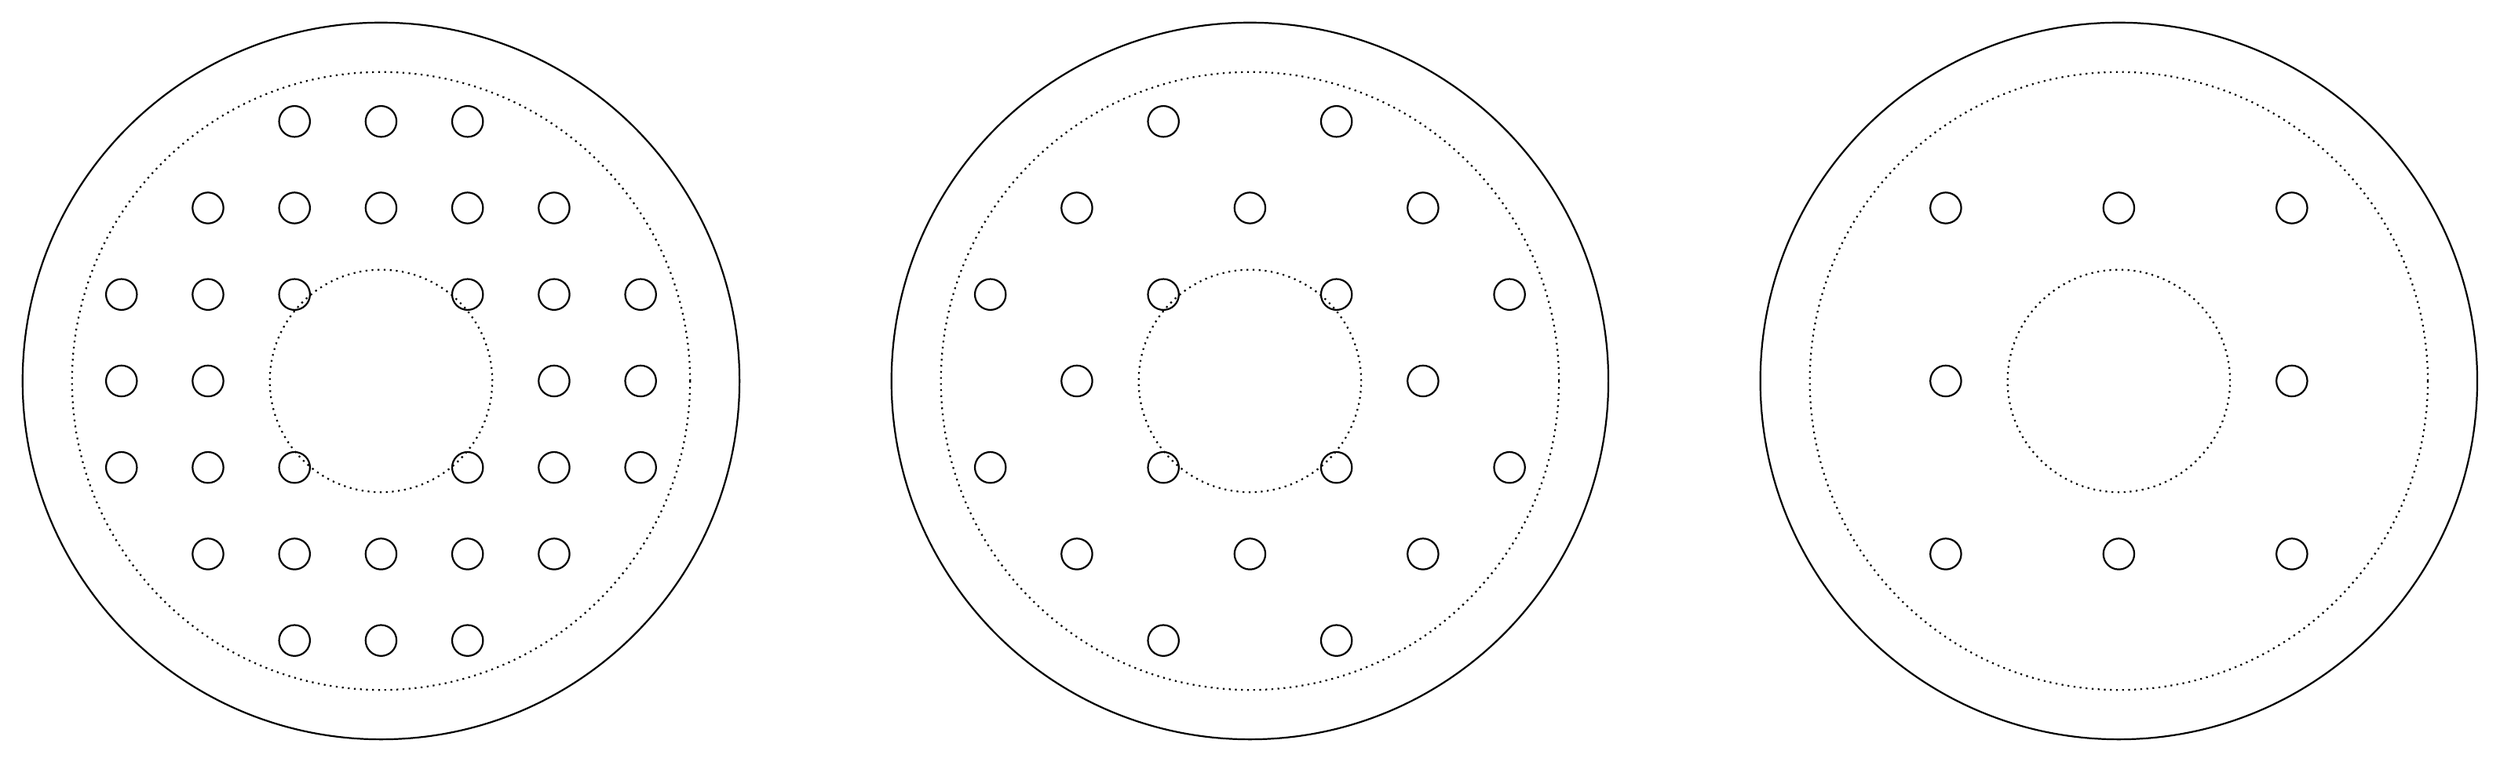
\begin{tikzpicture}[
 scale=0.2,
 thick
]
\begin{scope}[xshift=0,yshift=0]
\draw (0,0) circle (29);
\draw (+7,+7) circle (1.25);
\draw (+7,-7) circle (1.25);
\draw (-7,+7) circle (1.25);
\draw (-7,-7) circle (1.25);
\draw (0,+14) circle (1.25);
\draw (0,-14) circle (1.25);
\draw (+14,0) circle (1.25);
\draw (-14,0) circle (1.25);
\draw (+7,+14) circle (1.25);
\draw (-7,+14) circle (1.25);
\draw (+7,-14) circle (1.25);
\draw (-7,-14) circle (1.25);
\draw (+14,+7) circle (1.25);
\draw (+14,-7) circle (1.25);
\draw (-14,+7) circle (1.25);
\draw (-14,-7) circle (1.25);
\draw (+14,+14) circle (1.25);
\draw (+14,-14) circle (1.25);
\draw (-14,+14) circle (1.25);
\draw (-14,-14) circle (1.25);
\draw (-21,+7) circle (1.25);
\draw (-21,0) circle (1.25);
\draw (-21,-7) circle (1.25);
\draw (+21,+7) circle (1.25);
\draw (+21,0) circle (1.25);
\draw (+21,-7) circle (1.25);
\draw (+7,+21) circle (1.25);
\draw (0,+21) circle (1.25);
\draw (-7,+21) circle (1.25);
\draw (+7,-21) circle (1.25);
\draw (0,-21) circle (1.25);
\draw (-7,-21) circle (1.25);
\draw (0,0) [dotted] circle (25);
\draw (0,0) [dotted] circle (9);
\end{scope}
\begin{scope}[xshift=2000,yshift=0]
\draw (0,0) circle (29);
\draw (+7,+7) circle (1.25);
\draw (+7,-7) circle (1.25);
\draw (-7,+7) circle (1.25);
\draw (-7,-7) circle (1.25);
\draw (0,+14) circle (1.25);
\draw (0,-14) circle (1.25);
\draw (+14,0) circle (1.25);
\draw (-14,0) circle (1.25);
%\draw (+7,+14) circle (1.25);
%\draw (-7,+14) circle (1.25);
%\draw (+7,-14) circle (1.25);
%\draw (-7,-14) circle (1.25);
%\draw (+14,+7) circle (1.25);
%\draw (+14,-7) circle (1.25);
%\draw (-14,+7) circle (1.25);
%\draw (-14,-7) circle (1.25);
\draw (+14,+14) circle (1.25);
\draw (+14,-14) circle (1.25);
\draw (-14,+14) circle (1.25);
\draw (-14,-14) circle (1.25);
\draw (-21,+7) circle (1.25);
%\draw (-21,0) circle (1.25);
\draw (-21,-7) circle (1.25);
\draw (+21,+7) circle (1.25);
%\draw (+21,0) circle (1.25);
\draw (+21,-7) circle (1.25);
\draw (+7,+21) circle (1.25);
%\draw (0,+21) circle (1.25);
\draw (-7,+21) circle (1.25);
\draw (+7,-21) circle (1.25);
%\draw (0,-21) circle (1.25);
\draw (-7,-21) circle (1.25);
\draw (0,0) [dotted] circle (25);
\draw (0,0) [dotted] circle (9);
\end{scope}
\begin{scope}[xshift=4000,yshift=0]
\draw (0,0) circle (29);
%\draw (+7,+7) circle (1.25);
%\draw (+7,-7) circle (1.25);
%\draw (-7,+7) circle (1.25);
%\draw (-7,-7) circle (1.25);
\draw (0,+14) circle (1.25);
\draw (0,-14) circle (1.25);
\draw (+14,0) circle (1.25);
\draw (-14,0) circle (1.25);
%\draw (+7,+14) circle (1.25);
%\draw (-7,+14) circle (1.25);
%\draw (+7,-14) circle (1.25);
%\draw (-7,-14) circle (1.25);
%\draw (+14,+7) circle (1.25);
%\draw (+14,-7) circle (1.25);
%\draw (-14,+7) circle (1.25);
%\draw (-14,-7) circle (1.25);
\draw (+14,+14) circle (1.25);
\draw (+14,-14) circle (1.25);
\draw (-14,+14) circle (1.25);
\draw (-14,-14) circle (1.25);
%\draw (-21,+7) circle (1.25);
%\draw (-21,0) circle (1.25);
%\draw (-21,-7) circle (1.25);
%\draw (+21,+7) circle (1.25);
%\draw (+21,0) circle (1.25);
%\draw (+21,-7) circle (1.25);
%\draw (+7,+21) circle (1.25);
%\draw (0,+21) circle (1.25);
%\draw (-7,+21) circle (1.25);
%\draw (+7,-21) circle (1.25);
%\draw (0,-21) circle (1.25);
%\draw (-7,-21) circle (1.25);
\draw (0,0) [dotted] circle (25);
\draw (0,0) [dotted] circle (9);
\end{scope}
\end{tikzpicture}
}
\end{center}
\caption{The geometry of the Hartmann mask. The raw grid spacing is 70 mm (left). By covering holds with tape, this can be used to create less dense grids with spacings of 100 mm (center) and 140 mm (right).}
\label{figure:telescope-hartmann-mask-geometry}
\end{figure*}

We have constructed a Hartmann mask for the telescope. The mask has an array of 25 mm diameter holes on a Cartesian grid with a spacing of 70 mm between hole centers. By blocking holes with tape, one can create grids with spacings of 70, 100, and 140 mm (see Figure~\ref{figure:telescope-hartmann-mask-geometry}).

The mask is split into two to facilitate mounting. It should be secured to the secondary ring with cable ties and the joints between the two sections should be covered with tape. The telescope needs rebalancing in both axes after mounting the mask.

\subsection{Spherical Aberration}

In a conventional Hartmann test, one moves the detector and leaves the optical system fixed. However, this is not convenient here and we instead will move the secondary and leave the detector fixed. This will introduce spherical aberration. We have quantified this in ZEMAX using the nominal telescope design.

We placed a grid of rays on the pupil and then measured the radii $R_\mathrm{outer}$ and $R_\mathrm{inner}$ of the innermost and outermost points in the intrafocal and extrafocal images as function of the distance between M1 and M2. We interpolate the outer radii to zero to define the position of best focus. We then interpolate the inner radii to the same position determine the radius $R_\mathrm{inner}^\mathrm{best}$ of the image formed by the inner part of the pupil. We see that for images taken with the secondary moved $\pm1.0$, the spherical aberration amounts to 0.4 {\micron} or 0.02 arcsec radius in the interpolated best image plane. For images taken with the secondary moved $\pm1.5$, this rises to 2.0 {\micron} or 0.10 arcsec radius. 

The diffraction-limited image radius for the telescope in $B$ is $\lambda f/2D$ or about 1.8 {\micron} or 0.09 arcsec. Thus, for $\pm1.5$ mm displacement of the secondary, the spurious spherical aberration is small compared to the seeing but comparable to the diffraction limit and for $\pm 1.0$ mm displacement of the secondary, the spurious spherical aberration is small even compared to the diffraction limit. These should be borne in mind when determining the appropriate secondary displacement to use for a given application of the Hartmann test.

\begin{table}
\caption{Spherical Aberration in the Hartmann Test}
\label{table:hartmann-spherical-aberration}
\begin{center}
\begin{tabular}{ccccc}
\hline
\hline
$M1-M2$&$\Delta(M1-M2)$&$R_\mathrm{outer}$&$R_\mathrm{inner}$&$R_\mathrm{inner}^\mathrm{best}$\\
(mm)&(mm)&(\micron)&(\micron)&(\micron)\\
\hline
880.457&$-0.5$&343.3720&116.5\\
881.457&$+0.5$&343.372&117.2\\
&&&&0.7\\
\hline
879.957&$-1.0$&689.912&233.2\\
881.957&$+1.0$&688.212&234.1\\
&&&&0.7\\
\hline
882.457&$+1.5$&1033.26&351.9\\
879.457&$-1.5$&1033.93&350.1\\
&&&&2.0\\
\hline
\end{tabular}
\end{center}
\end{table}

\section{Bibliography}

\begin{flushleft}
\begin{itemize}
\item “\href{bibliography/astelco-telescope-technical-description.pdf}{Telescope Technical Description}”, ASTELCO.
\item “\href{bibliography/astelco-telescope-drawing-optics-section.pdf}{Drawing -- Optics Section}”, ASTELCO.
\item “\href{bibliography/astelco-telescope-drawing-instrument-flange-section.pdf}{Drawing -- Instrument Flange Section}”, ASTELCO.
\item “\href{bibliography/astelco-telescope-drawing-instrument-flange-plan.pdf}{Drawing -- Instrument Flange Plan}”, ASTELCO.
\end{itemize}
\end{flushleft}

%!TEX root = coatli.tex

\chapter{Secondary Focus Mechanism}
\label{chapter:secondary}

\section{Description}

\begin{figure*}
\begin{center}
\includegraphics[width=0.7\linewidth]{figures/secondary-coatli-mechanism.jpg}
\caption{The secondary focus mechanism with its cover removed.}
\label{figure:secondary-mechanism}
\end{center}
\end{figure*}

\begin{figure*}
\begin{center}
\begin{labeled}{\includegraphics[width=0.6\linewidth]{figures/secondary-coatli-controller.jpg}}
\arrowandlabel{(1.0,-2.4)}{(-0.9,-1.7)}{east}{Controller};
\end{labeled}
\caption{The secondary focus mechanism controller in the covers cabinet.}
\label{figure:secondary-controller}
\end{center}
\end{figure*}

The secondary mirror cell is mounted on a mechanism that allows it to move axially to focus the telescope.

The mechanism, shown in Figure~\ref{figure:secondary-mechanism}, appears to be an adaptation of an Optec TCF-S focuser. 

The controller for the secondary focus mechanism is located in the cabinet of the covers controller in the shed, and is shown in Figure~\ref{figure:secondary-controller}. Communication is via the Lantronix ethernet-to-serial server.

The mechanism does not appear to have an encoder, but rather appears to use a stepper motor and then count steps. The range of 0 to 7000 steps corresponds to 5.6 mm of motion (0.8 {\micron} per step), with 0 corresponding to the secondary at its lowest position (closest to the primary). The absolute calibration appears to be achieved by a combination of moving the motor to 7000 steps when it is powered on and a adjustable block and a hard stop that together define a reference position.

The position of the secondary cell on the focus mechanism can be adjusted manually.

TODO: Block diagram of hardware.

TODO: Control protocol.

\section{Maintenance Procedures}

\subsection{Static Adjustment of the Focus Range}
\label{section:secondary:static-adjustmentl}

This procedure describes how to statically adjust the range over which the secondary can be moved.

\begin{figure*}
\begin{center}
\begin{labeled}{\includegraphics[width=0.8\linewidth]{figures/secondary-coatli-adjustment.jpg}}
\arrowandlabel{(-0.4,-0.0)}{(-3.0,-2.2)}{east}{Hard Stop};
\arrowandlabel{(0.3,0.2)}{(3.0,-2.2)}{west}{Block};
\end{labeled}
\caption{The secondary focus mechanism adjustment. When the secondary focus mechanism is switched on, the mechanism moves upwards until the block comes into contact with the hard stop. This defines position 7000. The mechanism then moves back to 3400.}
\label{figure:secondary-adjustment}
\end{center}
\end{figure*}

\subsubsection{Safety Considerations}

\safety{Use a harness, line, and helmet when you work on the platform or balconies.}

\subsubsection{Requirements}

You will need:
\begin{itemize}
\item At least two persons.
\item The key to the shed (see \S\ref{section:shed-key}).
\item Metric hex keys. TODO: Size
\end{itemize}

\subsubsection{Procedure}

TODO: Photo.

\begin{enumerate}
\item Turn off power to the secondary controller, either by switching off power to the covers cabinet manually or by running
\begin{quote}
\verb|tcs request power switchoff secondary|
\end{quote}
\item Adjust the position of the block. When the secondary focus mechanism is switched on, the mechanism moves upwards until the block comes into contact with the hard stop. This defines position 7000. The mechanism then moves back to 3400. See Figure~\ref{figure:secondary-adjustment}.
\item Turn on the power to the secondary controller, either by switching on the covers cabinet manually or by running 
\begin{quote}
\verb|tcs request power switchon secondary|
\end{quote}
\end{enumerate}

\section{Remote Interface}

\subsection{Lantronix EDS}
\label{section:secondary-lantronix-eds}

The RS-232 interface to the secondary controller is made available via the Lantronix EDS 4100 ethernet-to-serial converter. Specifically, it is connected to line 2 and configured as 19200/8-N-1 with a tunnel on TCP port 10002.

The Lantronix EDS is on the LAN at \verb|serial|.

\section{Control}

The server for the secondary runs on \verb|control|. 

The server starts automatically after \verb|control| is boots, but if necessary can be stopped, started, or restarted explicitly by issuing the following shell commands on \verb|control|:
\begin{itemize}
\item
\verb|sudo stopserver secondary|
\item
\verb|sudo startserver secondary|
\item
\verb|sudo restartserver secondary|
\end{itemize}

Server requests can be issued from any of the Mac or Linux machines on the LAN. The following requests are supported:

\begin{itemize}
\item
\verb|request secondary initialize|

Initialize the server and secondary hardware. As part of the process of initializing, the secondary will more to its initial position.

For this request to be accepted, the server activity must not be \verb|starting| or \verb|error|.

If the request is accepted, the server activity changes to \verb|initializing| and then, once it has initialized, to \verb|idle|.

\item
\verb|request secondary move| \var{z0}

Move the secondary to position \var{z0}.

For this request to be accepted, the server activity must not be \verb|starting|, \verb|started|, \verb|initializing|, or \verb|error|.

If the request is accepted, the server activity changes to \verb|moving| and then, once it has opened to the specified angle, to \verb|idle|.

The nominal position \var{z0} is converted to a raw position by applying corrections for the filter, position, and temperature.

\item
\verb|request secondary stop|

Stop the secondary.

For this request to be accepted, the server activity must not be \verb|starting| or \verb|error|.

If the request is accepted, the server activity changes to \verb|stopping| and then, once it has stopped, to \verb|started| (if the server has not been initialized) or to the activity after the previous completed request.

\item
\verb|request secondary reset|

Reset an error in the secondary.


\item
\verb|request secondary status|

Show the status of the server.

Obtain the values of the status data from the server and print them to stdout.
\end{itemize}

\section{Bibliography}

\begin{flushleft}
\begin{itemize}
\item “\href{bibliography/secondary-coatli/tcs-f-manual.pdf}{TCS-F Technical Manual}”, Optec Inc, Revision 11, August 2010.
\end{itemize}
\end{flushleft}
\chapter{The Huitzi Imager}

The Huitzi imager was installed on the COATLI telescope in October 2021. The imager is named for the mexica god \href{https://en.wikipedia.org/wiki/Huītzilōpōchtli}{Huītzilōpōchtli}, the son of the goddess Coatlicue.

\section{Introduction}

The Huitzi imager has an Andor iXon electron-multiplying CCD detector with $1024\times1024$ pixels with a pixel scale of 0.68 arcsec and a field of 11.6 arcmin. The detector can be read through either a conventional amplifier or the electron-multiplying amplifier at a variety of speeds.

The image also has Finger Lakes Instruments filter wheel for eight 25 mm diameter filters. At the time of writing, the following filters are installed:
\begin{itemize}
    \item Pan-STARRS $griz$;
    \item 470/10, 640/10 continuum;
    \item 656/3 H$\alpha$; and
    \item a dark filter.
\end{itemize}

The mounting hardware for the Huitzi imager is adapted from the previous interim imager (see Appendix~\ref{appendix:interim-imager}).

\section{Hardware}

\begin{figure*}
\begin{center}
\includegraphics[width=0.45\linewidth]{figures/huitzi-hardware.jpg}
\includegraphics[width=0.45\linewidth]{figures/huitzi-hardware-telescope.jpg}
\includegraphics[width=0.675\linewidth]{figures/huitzi-hardware-electronics.jpg}
\end{center}
\caption{The Huitzi hardware. On the telescope the principal components are the Andor iXon detector and FLI filter wheel. The control electronics are located in the box mounted on the south side of the pillar. The cables pass up onto the telescope through an Igus Triflex chain.}
\label{figure:huitzi-hardware}
\end{figure*}

The hardware of the Huitzi instrument is shown in Figure~\ref{figure:huitzi-hardware}. On the telescope the principal components are the Andor iXon detector and FLI filter wheel. The control electronics are located in the box mounted on the south side of the pillar. The cables pass up onto the telescope through an Igus Triflex chain.

\subsection{Detector}

The detector unit is an Andor iXon Ultra 888 with an e2v CCD201-20 electron-multiplying CCD detector. The detector was acquired in 2014 and originally intended to be the tilt sensor for the planned two-channel imager.

The detector has $1024\times1024$ pixels each $13\times13$ {\micron} square. It gives a pixel scale of 0.68 arcsec and a field of 11.6 arcmin. 

The detector has standard silicon and the e2v midband coating (which in Andor's terminology makes it a “BV” device).

The detector can be read using either a conventional signal chain (at 100 kHz or 1 MHz) or an EM signal chain (at 1, 10, 20, or 30 MHz). Both chains have two gains and the EM gain can be set to up to 1000. The detector also has a frame-transfer capability.

The detector has a conventional mechanical iris shutter. We originally used the mechanical shutter for conventional CCD modes and the frame-transfer capability for EM modes. However, we found that the shutter sometimes failed to open or failed to open completely. We suspect that at the colder temperatures at night, the power supply does not provide sufficient voltage. Therefore, we now leave the shutter open permanently and use the frame-transfer capability in both conventional and EM modes. To take bias and dark images, we have installed a “dark” filter (a opaque cylinder of Delrin 25 mm in diameter and 5 mm thick) in the filter wheel. 

With the normal vertical-shift frequency of 4.33 MHz, the frame transfer takes about 4.5 ms. This leads to some trailing above and below bright stars.

\subsection{Filter Wheel}

The slots are filled as follows:
    \begin{enumerate}
        \item[0:] $g$
        \item[1:] $r$
        \item[2:] $i$
        \item[3:] $z$
        \item[4:] 470/10
        \item[5:] dark
        \item[6:] 640/10
        \item[7:] 656/3
    \end{enumerate}
    
\subsection{Filters}


\subsection{Mounting Hardware}

\subsection{Control Hardware}

\section{Control Software}

\section{Maintenance Procedures}

\subsection{Dismounting and Mounting the Instrument}
\label{section:huitzi-dismounting-and-mounting}

\subsubsection{Requirements}

You will need:

\begin{itemize}
    \item Two persons.
    \item The key to the shed (see \S\ref{figure:buildings-shed-key}).
    \item 4 mm and 2 mm hex keys
    \item 5/16 inch hex key.
\end{itemize}

\subsubsection{Dismounting the Imager}

\begin{figure*}
\begin{center}
\includegraphics[width=0.8\linewidth]{figures/huitzi-detector-power-button.jpg}
\end{center}
\caption{The detector power button.}
\label{figure:huitzi-detector-power-button}
\end{figure*}

\begin{figure*}
\begin{center}
\includegraphics[width=0.8\linewidth]{figures/huitzi-cables-disconnected.jpg}
\end{center}
\caption{The disconnected detector and filter wheel USB and power cables.}
\label{figure:huitzi-cables-disconnected}
\end{figure*}

\begin{figure*}
\begin{center}
\includegraphics[width=0.8\linewidth]{figures/huitzi-mounting-screws.jpg}
\end{center}
\caption{The six screws that hold the filter wheel and detector to the separator barrel. Note the arrow scratched on the separator barrel that aligns with a similar barrel on the front filter wheel plate.}
\label{figure:huitzi-mounting-screws}
\end{figure*}

\begin{figure*}
\begin{center}
\includegraphics[width=0.8\linewidth]{figures/huitzi-off-telescope.jpg}
\end{center}
\caption{The dismounted detector and filter wheel resting on the rear surface of the detector. The six screws that hold the filter wheel between the front and rear plates can be seen here.}
\label{figure:huitzi-off-telescope}
\end{figure*}

\begin{figure*}
\begin{center}
\includegraphics[width=0.3\linewidth]{figures/huitzi-operating-off-telescope-a.jpg}
\includegraphics[width=0.3\linewidth]{figures/huitzi-operating-off-telescope-b.jpg}
\includegraphics[width=0.3\linewidth]{figures/huitzi-operating-off-telescope-c.jpg}
\end{center}
\caption{Operating the instrument off the telescope. Disconnect the Igus Triflex chain, remove the white secondary cable, connect the instrument, and press the power button on the detector..}
\label{figure:huitzi-operating-off-telescope}
\end{figure*}

\begin{figure*}
\begin{center}
\includegraphics[width=0.8\linewidth]{figures/huitzi-set-screws-a.jpg}
\includegraphics[width=0.8\linewidth]{figures/huitzi-set-screws-b.jpg}
\end{center}
\caption{The two set screws in the filter wheel.}
\label{figure:huitzi-set-screws}
\end{figure*}


\begin{figure*}
\begin{center}
\includegraphics[width=0.8\linewidth]{figures/huitzi-without-front-plate.jpg}
\end{center}
\caption{The detector and filter wheel without the front plate.}
\label{figure:huitzi-without-front-plate}
\end{figure*}

\begin{figure*}
\begin{center}
\includegraphics[width=0.8\linewidth]{figures/huitzi-without-spacer.jpg}
\end{center}
\caption{The detector and filter wheel without the spacer.}
\label{figure:huitzi-without-spacer}
\end{figure*}

\begin{figure*}
\begin{center}
\includegraphics[width=0.8\linewidth]{figures/huitzi-without-filter-wheel.jpg}
\end{center}
\caption{The detector without the filter wheel, revealing the rear plate and the rear light baffle cone.} 
\label{figure:huitzi-without-filter-wheel}
\end{figure*}

\begin{figure*}
\begin{center}
\includegraphics[width=0.8\linewidth]{figures/huitzi-without-rear-cone.jpg}
\end{center}
\caption{The detector without the rear light baffle cone. The four screws that hold the rear plate to the detector can be seen here. Note that the holes for the screws are indicated with scratched lines.}
\label{figure:huitzi-without-rear-cone}
\end{figure*}

\begin{enumerate}

    \item Go to the shed. Put on harnesses and helmets. Move the enclosure switch to LOCAL. Open the enclosure to 60 degrees. Ascend to the platform.

    \item Move the telescope to the home position (above the mount and pointed at the north pole). To do this, press the brake button and move the telescope by hand. This is important, as after the instrument is removed the telescope will not be balanced.

    \item Turn off the detector by pressing the power button on its underside. See Figure~\ref{figure:huitzi-detector-power-button}.

    \item Disconnect the four cables: detector USB and power and filter wheel USB and power (see Figure~\ref{figure:huitzi-cables-disconnected}).

    \item Dismount the filter wheel and detector by removing the six screws that hold them to the separator barrel. See Figure~\ref{figure:huitzi-mounting-screws}. Use a 4 mm hex key.  One person should support the filter wheel and detector while the other removes the screws.

    \item Place the filter wheel and detector in a safe place resting on the rear surface of the detector. The covered end of the enclosure is ideal. See Figure~\ref{figure:huitzi-off-telescope}.

    \item If you do not need to operate the instrument when dismounted, skip this step.
    
    If you do need to operate the instrument when dismounted, the easiest approach is place the instrument on the steps just to the south of the columm. Be careful that the steps do not penetrate the duct-taped gap between the column and the platform.
    Then, disconnect the Igus Triflex chain from the telescope and remove the white secondary cable. Finally, connect the detector and filter wheel cables to the instrument and press the power button on the detector. See Figure~\ref{figure:huitzi-operating-off-telescope}.
    
    \item If you do not need access to the filter wheel and/or detector, stop here.  If you do, continue.
    
    \item Remove the two set screws between the filter wheel and the detector. Use a 5/16 inch hex key. See Figure~\ref{figure:huitzi-set-screws}.
    
    \item Remove the the six screws that pass from the front plate, through the wheel, and into the rear plate. Use a 2 mm hex key. See Figure~\ref{figure:huitzi-off-telescope}.
    
    \item Remove the front plate to expose the filter wheel and spacer. See Figure~\ref{figure:huitzi-without-front-plate}.
    
    \item Remove the spacer to expose the filter wheel. See Figure~\ref{figure:huitzi-without-spacer}.
    
    \item Remove the filter wheel. See Figure~\ref{figure:huitzi-without-filter-wheel}.
    
    \item If you do not need access to the detector, stop here. If you do, continue.
    
    \item Remove the rear light baffle cone from the rear plate. It is held in place by friction.  See Figure~\ref{figure:huitzi-without-filter-wheel}. 
    
    \item Remove the four screws that hold the rear plate to the detector flange. Use a 4 mm hex key. See Figure~\ref{figure:huitzi-without-rear-cone}.

\end{enumerate}

\subsubsection{Mounting the Imager}

\begin{enumerate}

    \item Go to the shed. Put on harnesses and helmets. Move the enclosure switch to LOCAL. Open the enclosure to 60 degrees. Ascend to the platform.

    \item Replace the four screws that hold the rear plate to the detector flange. Use a 4 mm hex key. The correct holes for the screws are indicated with scratches on the rear plate. Note the orientation of the plate. See Figure~\ref{figure:huitzi-without-rear-cone}.

    \item Replace the rear light baffle cone from the rear plate.See Figure~\ref{figure:huitzi-without-filter-wheel}. 

    \item Replace the filter wheel. See Figure~\ref{figure:huitzi-without-filter-wheel}.

    \item Replace the spacer. See Figure~\ref{figure:huitzi-without-front-plate}.
    
    \item Replace the front plate. See Figure~\ref{figure:huitzi-off-telescope}.
    
    \item Replace the the six screws that pass from the front plate, through the wheel, and into the rear plate. Use a 2 mm hex key. See Figure~\ref{figure:huitzi-off-telescope}.

    \item Replace the two set screws between the filter wheel and the detector. Use a 5/16 inch hex key. See Figure~\ref{figure:huitzi-set-screws}.

    \item Mount the filter wheel and detector by replacing the six screws that hold them to the separator barrel. See Figure~\ref{figure:huitzi-mounting-screws}. Use a 4 mm hex key. One person should support the filter wheel and detector while the other replaced the screws. Note the orientation of the filter wheel and detector. The arrows scratched on the separator barrel and front plate should be aligned.

   \item Connect the four cables: detector USB and power and filter wheel USB and power (see Figure~\ref{figure:huitzi-cables-disconnected}).

   \item Turn on the detector by pressing the power button on its underside. See Figure~\ref{figure:huitzi-detector-power-button}.

\end{enumerate}

\subsection{Changing a Filter}

\subsubsection{Requirements}

You will need:

\begin{itemize}
    \item Two persons.
    \item The key to the shed.
    \item 4 mm and 2 mm hex keys (to dismount and mount the instrument).
    \item 5/16 inch hex key (to dismount and mount the instrument).
    \item A clean plastic bag to transport the filter wheel. There are bags in the COATLI/DDOTI tool cabinet.
    \item PH1 screwdriver.
    \item Tweezers
    \item Nitrile gloves
    \item If replacing a 5 mm filter with a 3 mm filter, one of the 25 mm O-rings supplied with the filter wheel.
\end{itemize}

\subsubsection{Procedure}

\begin{figure*}
\begin{center}
\includegraphics[width=0.8\linewidth]{figures/huitzi-filter-wheel-slots.jpg}
\end{center}
\caption{The filter wheel. There are 8 filter slots, labelled 0 to 7. The filter wheel can be moved by hand.}
\label{figure:huitzi-filter-wheel-slots}
\end{figure*}

\begin{figure*}
\begin{center}
\includegraphics[width=0.8\linewidth]{figures/huitzi-filter-paper.jpg}
\end{center}
\caption{The filters are wrapped in optical paper.}
\label{figure:huitzi-filter-paper}
\end{figure*}

\begin{figure*}
\begin{center}
\includegraphics[width=0.8\linewidth]{figures/huitzi-filter-case.jpg}
\end{center}
\caption{The filters are protected by cases like this one.}
\label{figure:huitzi-filter-case}
\end{figure*}

\begin{figure*}
\begin{center}
\includegraphics[width=0.6\linewidth]{figures/huitzi-filter-wheel-o-ring-a.jpg}
\includegraphics[width=0.6\linewidth]{figures/huitzi-filter-wheel-o-ring-b.jpg}
\end{center}
\caption{The difference in thickness between the 3 mm and 5 mm thick filters is compensated by an O-ring.}
\label{figure:huitzi-filter-wheel-o-ring}
\end{figure*}

\safety{Filters are delicate optical components. Work in the laminar-flow cabinet at the 2.1 meter. Handle them by their edges. They should only be cleaned by optical engineers.}

\safety{Do not remove dust from filters by blowing them with compressed air from a compressor, cylinder, or can, as these sources can contain oil. Only use a hand blower (perilla).}

\begin{enumerate}
    \item Remove the filter wheel from the instrument. See \S\ref{section:huitzi-dismounting-and-mounting}.
    \item Place the filter wheel in the clean plastic bag. Take the filter wheel to the optical workshop at the 2.1 meter. Replace the filters in the laminar-flow cabinet to avoid dust.
    \item Use nitrile gloves.
    \item Move the filter wheel by hand to expose the correct filter. See Figure~\ref{figure:huitzi-filter-wheel-slots}. The 8 filter slots are labelled from 0 to 7.
    \item Remove the two screws and washers that hold the filter in place. See Figure~\ref{figure:huitzi-filter-wheel-slots}.  Use the PH1 screwdriver and the tweezers.
    \item Use one finger to push the filter from below and the other hand to remove the filter.
    \item Wrap the filter in optical paper (which should be in its box). See Figure~\ref{figure:huitzi-filter-paper}.
    \item Replace the filter in its case. See Figure~\ref{figure:huitzi-filter-case}.
    \item If you are replacing a 5 mm thick filter ($griz$ and $BVRI$) with a 3 mm thick filter (the medium-band $XXX$/10 and narrow-band $XXX$/3 filters), place a 25 mm O-ring in the filter slot. See Figure~\ref{figure:huitzi-filter-wheel-o-ring}.
    
    If you are replacing a 3 mm thick filter with a 5 mm filter, remove the 25 mm O-ring from the slot and store it the ziploc bag that contains the others.
    
    \item Place the filter in the slot. For interference filters (all but $BVRI$), the bandpass coating (which will often appear to be reflective) should be on the side towards the filter wheel motor. This is down in the orientation shown in \ref{figure:huitzi-filter-wheel-slots} but up once the filter wheel is installed on the telescope.
    
    \item Replace the  two screws and washers that hold the filter in place. See Figure~\ref{figure:huitzi-filter-wheel-slots}.  Use the PH1 screwdriver and the tweezers. The washers should make contact with the filter. We find it is easiest to insert both screws first without tightening either and then tighten each in turn. You can use tweezers to make sure the washers are positioned correctly.
    
    \item If necessary, use a hand blower (perilla) to remove dust from the filter surfaces.
    
    \item Make sure the filter wheel can turn without the screws interfering with the casing. Do this by turning the filter wheel by hand.
    
    \item Place the filter wheel in the clean plastic bag. Return it to the platform.
    
    \item Replace the filter wheel in the instrument. See \S\ref{section:huitzi-dismounting-and-mounting}.

\section{Bibliography}

\begin{flushleft}
\begin{itemize}
\item “\href{bibliography/huitzi/andor-ixon-ultra-888-data-sheet.pdf}{Andor iXon Ultra 888 Data Sheet}”, Andor, May 2014.
\item “\href{bibliography/huitzi/andor-ixon-ultra-888-hardware-guide.pdf}{Andor iXon Ultra \& Life 888 Hardware Guide}”, Andor, Version 1.8 of 30 September 2019.
\item “\href{bibliography/huitzi/e2v-ccd201-20-datasheet.pdf}{CCD201-20 Datasheet}”, Teledyne e2v, Version 7 of August 2019.
\end{itemize}
\end{flushleft}
    
\end{enumerate}
\chapter{Calibrations}

This chapter describes the routine calibrations procedures for {\projectname}.

\part{Control System}

\chapter{Control System}
\label{chapter:control-system}

TODO: What runs where.

TODO: Structure.

TODO: stopserver/startserver/restartserver

TODO: restartsoon (haltsoon and rebootsoon in network)

TODO: state and activity

TODO: basic requests: initialize, status, reset, stop

TODO: supervisor\\
request supervisor enable/disable/open/close/emergencyclose

TODO: Detectors:\\
expose <time> object/dark/bias/flat\\
setcooler on/off\\
movefilterwheel position/filter\\
movefocuser position \\
setfocuser position
setwindow 1kx1k/2kx2k/6kx6k/default/full\\
setbinning 1/2/4 \\
setreadmode mode \\
setsoftwaregain \\
focus TBD \\
analyze fwhm/levels

TODO: selector\\
request selector enable/disable \\
request select setunfocused

TODO: instrument\\
open/close

TODO: telescope\\
park\\
unpark\\
move HA dec \\
newtrack RA dec equinox \\
newtracktopocentric HA dec \\
01:23:45.67 +3h 60d \\
open/close

TODO: executor\\
open/close

TODO: \\
request telescope emergencyclose \\
sudo restartsoon \\
request supervisor enable
\chapter{JSON}

JSON is used widely in TCS to represent data structures in configuration files, alert files, block files, and in inter-process communication. JSON has a simple and regular syntax that is fairly easy for humans to write, easy for computers to parse, and should be quite familiar to C, C++, and JavaScript programmers. 

\section{Dialect}

The dialect of JSON used in TCS is both extended and restricted compared to standard JSON.

It is extended by the addition of comment lines that can appear wherever white-space can appear in standard JSON. A comment line is a line that begins with zero or more space and horizontal tab characters followed by two slash characters (“//”). Formally, the slash character is U+002F SOLIDUS. Other types of comments (e.g., block comments introduced by “/*” and terminated by “*/”) are not allowed. Comment lines are treated as if they were empty lines. Our dialect of JSON can be converted to standard JSON by using a regular expression substitution to replace comment lines with empty lines.

It is restricted with respect to standard JSON in that it only uses array, object, and string values and does not use number, true, false, or null values. If a value represents a number, then the string representation should be used. This restriction ensures that value can be read and written without being changed.

The dialect of JSON is formally a very limited subset of JavaScript. Therefore, if you are editing data files manually, it might be useful to select an editing mode suitable for JavaScript.

\section{Encoding}

Data files should be encoded in UTF-8. ASCII is a subset of UTF-8, but ISO-8859-1 “Latin-1” is not.

\section{Values}

\subsection{Value Types}

Only array, object, and string values are used. Number and boolean values are represented by their string representation. For example, we do not write
\begin{quote}
\verb|0|\\
\verb|true|\\
\verb|false|\\
\end{quote}
but rather 
\begin{quote}
\verb|"0"|\\
\verb|"true"|\\
\verb|"false"|\\
\end{quote}
Null values are not used.

\subsection{Dates and Times}

Dates and time values are written as strings containing an IS0-8601 basic date or basic combined date and time.
The time zone is understood to be UTC; an explicit time zone must not be specified. The precision must not be specified more finely than seconds.

Examples of valid dates are:
\begin{quote}
\verb|"20101117T223815"| : 2010 Nov 17 22:38:15 UTC\\
\verb|"20101117T2238"  | : 2010 Nov 17 22:38:00 UTC\\
\verb|"20101117T22"    | : 2010 Nov 17 22:00:00 UTC\\
\verb|"20101117"       | : 2010 Nov 17 00:00:00 UTC
\end{quote}

\subsection{Angles}
\label{section:angles}

A value representing an angle may be written as:

\begin{enumerate}
    \item a string containing a decimal number (and interpreted as \emph{radians} not \emph{degrees});
    \item a string containing sexagesimal notation with colons as separators and no white space;
    \item a strings containing a decimal number with a unit suffix (with no intermediate white space):
    \begin{enumerate}
        \item “r” for radians;
        \item “h” for hours;
        \item “m” for minutes;
        \item “s” for seconds;
        \item "ad" or “d” for degrees;
        \item “am” for arcminutes; and
        \item “as” for arcseconds.
    \end{enumerate}
\end{enumerate}

For hour angles and right ascensions, sexagesimal notation indicates hours, minutes, and seconds. For all other angles, including offsets, it indicates degrees, arcminutes, and arcseconds.

Examples of valid angles are:
\begin{quote}
\verb|"-22.5"    | : $-22.5$ \emph{radians}\\
\verb|"-22.5d"   | : $-22.5$ \emph{degrees}\\
\verb|"-01:30:00"| : $-1.5$ hours or $-1.5$ degrees, depending on the context\\
\verb|"0.5r"     | : $0.5$ radians\\
\verb|"-1.5h"    | : $-1.5$ hours\\
\verb|"5am"      | : $5$ arcminutes\\
\verb|"+20as"    | : $20$ arcseconds
\end{quote}

\subsection{Durations}

A value representing a duration may be written as:
\begin{enumerate}
\item a string containing a decimal number (and interpreted as decimal seconds);
\item a string containing sexagesimal notation with colons as separators and no white space;
\item a string containing a decimal number with a unit suffix (with no intermediate white space):
\begin{enumerate}
    \item “h” for hours;
    \item “m” for minutes; and
    \item “s” for seconds.
\end{enumerate}
\end{enumerate}

Sexagesimal notation indicates hours, minutes, and seconds.

Examples of valid durations are:
\begin{quote}
\verb|"60"      | :	60 seconds\\
\verb|"00:30:10”| : 30 minutes and 10 second\\
\verb|"60s"		| :	60 seconds\\
\verb|"10m"		| :	10 minutes\\
\verb|"1h"		| :	1 hour
\end{quote}

\subsection{Validation}

JSON written by hand is prone to errors such as missing commas. For this reason, it is often worthwhile checking JSON with one of the many on-line validators. The following validator is especially useful, as it tolerates comments:

\begin{quote}
\url{https://jsonformatter.curiousconcept.com/#}
\end{quote}

\section{Bibliography}

\begin{itemize}
    \item “Introducting JSON”, \url{https://www.json.org/json-en.html}
\end{itemize}
\chapter{Observing Blocks}

\section{Introduction}

Observations are organized as \emph{project}, \emph{blocks}, and \emph{visits}.

A project is associated with a successful observing proposal. It has a PI, a name, and an identifier. It consists of one or more blocks.

A block consists of a ordered set of visits associated with a set of constraints and a program. The selector and executor deal with blocks: the selector selects a block and the executor executes it. A block is only selectable if all of its visits satisfy all of the constraints. When a block is executed, its visits are carried out in order.

A visit is typically a logical operation with the telescope such as focusing, correcting the pointing, or observing an objects.

\section{Block Files}

A block file contains a JSON representation of a block.

It consists of a single JSON object with the following structure:
\begin{quote}
\verb|{|\\
\verb|  "project": {|\\
\verb|    "identifier":| <project-identifier>\verb|,|\\
\verb|    "name":| <project-name>\\
\verb|  },|\\
\verb|  "identifier":| <block-identifier>\verb|,|\\
\verb|  "name":| <block-name>\verb|,|\\
\verb|  "visits":| <visits>\verb|,|\\
\verb|  "constraints":| <constraints>\verb|,|\\
\verb|  "persistent":| <persistent>\\
\verb|}|
\end{quote}

As for any JSON object, the order of the members is irrelevant.

The members and values are interpreted as follows:

\begin{itemize}
    \item <project-identifier>: The project identifier. 
    
    This is a four-digit non-negative integer represented as a string. 
    
    By convention, calibration programs have identifiers from 0000 to 0999, alert science programs from 1000 to 1999, and non-alert science programs from 2000 to 2999. (The pipeline uses this convention to reduce alert observations immediately but delay reducing non-alert observations until the morning.) 
    
    This member cannot be omitted.
    
    \item <project-name>: The project name. 
    
    By convention, we use the surname of the PI followed by a brief description of the objects (e.g., \verb|"Watson YSOs"|). 
    
    If omitted, the default is \verb|""|.

    \item <block-identifier>: The block identifier. 
    
    This is a non-negative integer represented as a string. 
    
    This member cannot be omitted.

    \item <block-name>: The block name.
    
    By convention, we briefly describe the main science target (e.g., \verb|"HL Tau"|). 
    
    If omitted, the default is \verb|""|.

    \item <visits>: An array representing the visits. See below. 
    
    If omitted, the default is an empty array.
    
    \item <constraints>: An object representing the constraints. See below. 
    
    If omitted, the default is an empty object.

    \item <persistent>: Whether the block is persistent.
    
    Either \verb|"true"| or \verb|"false"|. 
    
    If \verb|"true"|, the block is persistent. Persistent blocks remain in the queue after they have been executed. Non-persistent blocks are removed after they have been executed.
    
    If omitted, the default is \verb|"false"|.

\end{itemize}

\section{Constraints}

The <constraints> value specifies constraints which shall be satisfied by all of the visits in a block in order for the block to be selectable. If any constraint is not satisfied by any visit, the block will not be selectable.

For a block to be selectable:
\begin{itemize}
    \item All time-based constraints (\verb|mindate|, \verb|maxdate|, \verb|minfocusdelay|, and \verb|maxfocusdelay|) must be satisfied at the start of the first visit.
    \item All condition-based constraints (e.g., on transparency) must be satisfied at the start of the first visit.  (In the present version of the selector, there are no constraints on unpredictable properties, but this may change in future versions.)
    \item All other constraints must be satisfied at the start and end of \emph{each} visit.
\end{itemize}

Syntactically, the <constraints> value is a JSON object with the following structure:
\begin{quote}
\verb|{|\\
\verb|  "mindate":| <date>\verb|,|\\
\verb|  "maxdate":| <date>\verb|,|\\
\verb|  "minsunha":| <ha>\verb|,|\\
\verb|  "maxsunha":| <ha>\verb|,|\\
\verb|  "minsunzenithdistance":| <distance>\verb|,|\\
\verb|  "maxsunzenithdistance":| <distance>\verb|,|\\
\verb|  "minmoondistance":| <distance>\verb|,|\\
\verb|  "maxmoondistance":| <distance>\verb|,|\\
\verb|  "minha":| <ha>\verb|,|\\
\verb|  "maxha":| <ha>\verb|,|\\
\verb|  "mindelta":| <delta>\verb|,|\\
\verb|  "maxdelta":| <delta>\verb|,|\\
\verb|  "minairmass":| <airmass>\verb|,|\\
\verb|  "maxairmass":| <airmass>\verb|,|\\
\verb|  "minzenithdistance":| <distance>\verb|,|\\
\verb|  "maxzenithdistance":| <distance>\verb|,|\\
\verb|  "minskybrightness":| <skybrightness>\verb|,|\\
\verb|  "maxskybrightness":| <skybrightness>\verb|,|\\
\verb|  "minfocusdelay":| <delay>\verb|,|\\
\verb|  "maxfocusdelay":| <delay>\verb|,|\\
\verb|}|
\end{quote}

As for any JSON object, the order of the members is irrelevant.

The members and values are interpreted as follows:

\begin{itemize}

\item The <mindate> and <maxdate> values specify the earliest and latest date and time on which to the visit shall be executed.

Valid values are dates.

\item The <minsunha> and <maxsunha> values specify the minimum and maximum values of the HA of the Sun.

Valid values are angles.

These are of most interest to calibration blocks, where these can be used to determine whether it is morning or evening.

\item The <minsunzenithdistance> and <maxsunzenithdistance> values specify the minimum and maximum values of the zenith distance of the Sun.

Valid values are angles.

These are of most interest to calibration blocks.

\item The <minmoondistance> and <maxmoondistance> members specify the minimum and maximum values of the distance of the Moon from the visit targets.

Valid values are angles.

\item
The <minha> and <maxha> values specify the minimum and maximum values of the HA of the visit targets.

Valid values are angles.

These can be used to program several blocks on the same target in the a given night by giving each a HA range disjoint from the others.

\item
The <mindelta> and <maxdelta> values specify the minimum and maximum values of the declination of the visit targets.

Valid values are angles.

\item 
The <minairmass> and <maxairmass> members specify the minimum and maximum values of the zenith distance of the visit targets.

Valid values are numbers.

\item 
The <minzenithdistance> and <maxzenithdistance> values specify the minimum and maximum values of the zenith distance of the visit targets.

Valid values are angles.

\item The <minskybrightness> and <maxskybrightness> values specify the minimum (faintest) and maximum (brightest) sky brightness in which the visit shall be executed. 
    
Valid values are: \verb|"daylight"|, \verb|"civiltwilight"|, \verb|"nauticaltwilight"|, \verb|"astronomicaltwilight"|, \verb|"bright"|, \verb|"grey"|, and \verb|"dark"|. 
    
Daylight and the twilights are defined conventionally by the altitude of the Sun. Bright time is any time between twilights when the moon is above the horizon and is 50\% illuminated or more. Grey time is s any time between twilights when the moon is above the horizon and is 50\% illuminated or less. Dark time is any time between twilights when the moon is below the horizon.
    
\item
The <minfocusdelay> and <maxfocusdelay> values specify the minimum and maximum time since the telescope was last focused. So, for example specifying a <minfocusdelay> of \verb|"1h"| will constrain the block to be run no sooner than 1 hour after focusing and specifying a maxfocusdelay of \verb|"1h"| will constrain the block to be run no later than 1 hour after focusing.

Valid values are durations.

These are of most interest to focus blocks.

\end{itemize}

In addition to any explicit constraints, the scheduler requires that all visit targets are within the telescope pointing limits at the expected start and of the visit.

If no explicit constraints are given, the implicit telescope pointing limits are the only constraint and, for example, a block may be executed at very high airmass, close to the mount, or during twilight. Therefore, it is advisable to include at least minimal constraints, for example:
\begin{quote}
\begin{verbatim}
{
  "maxskybrightness": "astronomicaltwilight",
  "maxairmass": "2.0",
  "minmoondistance": "15d"
}
\end{verbatim}
\end{quote}

\section{Visits}

Syntactically, the <visits> value is a JSON array containing zero or more <visit> objects:
\begin{quote}
\verb|[|\\
\verb|  |<visit>\verb|,|\\
\verb|  |<visit>\verb|,|\\
\verb|  |<visit>\verb|,|\\
\verb|  |\ldots\\
\verb|  |<visit>\\
\verb|]|
\end{quote}

Each <visit> value is a JSON object with the following structure:
\begin{quote}
\verb|{|\\
\verb|  "identifier":| <visit-identifier>\verb|,|\\
\verb|  "name":| <visit-name>\verb|,|\\
\verb|  "targetcoordinates":| <target-coordinates>\verb|,|\\
\verb|  "estimatedduration":| <estimated-duration>\verb|,|\\
\verb|  "command":| <command>\\
\verb|}|
\end{quote}

As for any JSON object, the order of the members is irrelevant.

The members and values are interpreted as follows:

\begin{itemize}
\item <visit-identifier>: The visit identifier.

This is a non-negative integer represented as a string.

By convention, science visits have identifiers from 0 to 999 and focusing, pointing correction, and other non-science visits from 1000 onward. (The pipeline uses this convention to avoid reducing non-science visits.)

\item <visit-name>: The visit name.

By convention, we used names that describe the activity generically, such as \verb|"focussing"|, \verb|"pointingcorrection"|, \verb|"science"|.

If omitted, the default is \verb|""|.

\item <target-coordinates>: The target coordinates. See below.

\item <estimated-duration>: The estimated duration of the visit.

Valid values are durations (e.g., \verb|"10m"| for 10 minutes).

This is used to by the selector to check the constraints at the estimated end of the visit.

\item <command>: The command to execute the visit. See below.

\end{itemize}

\section{Target Coordinates}

The <target-coordinates> value is a JSON object with one of the following structures.

For equatorial coordinates, the structure is:
\begin{quote}
\verb|{|\\
\verb|  "type": "equatorial",|\\
\verb|  "alpha":| <alpha>\verb|,|\\
\verb|  "delta":| <delta>\verb|,|\\
\verb|  "equinox":| <equinox>\\
\verb|}|
\end{quote}

The <alpha> and <delta> values are angles. The <equinox> value is a number.

For fixed topocentric coordinates, the structure is:
\begin{quote}
\verb|{|\\
\verb|  "type": "fixed",|\\
\verb|  "ha":| <ha>\verb|,|\\
\verb|  "delta":| <delta>\\
\verb|}|
\end{quote}

The <ha> and <delta> values are angles.

For the zenith, the structure is:
\begin{quote}
\verb|{|\\
\verb|  "type": "zenith"|\\
\verb|}|
\end{quote}

For the idle position, the structure is:
\begin{quote}
\verb|{|\\
\verb|  "type": "idle"|\\
\verb|}|
\end{quote}

For a solar system body, the structure is:
\begin{quote}
\verb|{|\\
\verb|  "type": "solarsystembody",|\\
\verb|  "number":| <number>\\
\verb|}|
\end{quote}

The <number> is a number and refers to the number part of the minor-planet designation. For example, for  (388188) 2006 DP$_{14}$, it would be \verb|388188|.

\section{Commands}

The <command> value is a string representing the Tcl command that will be run to execute the visit. Here we describe the three main commands of interest to science blocks and omit the other commands that are used in calibration blocks.

Many parameters of commands have default values.

\subsection{Focus}

The \verb|focusvisit| command focuses 
\ifcoatlioan
the secondary on C0.
\fi
\ifddotioan
the focuser of each channel C0 to C5.
\fi

The parameters are:
\begin{itemize}
    \item \verb|filter|: the filter in which to focus. The default is \verb|i|.
    \item \verb|exposuretime|: the exposure time in seconds. The default is \verb|5|.
\end{itemize}

Examples:
\begin{quote}
\begin{verbatim}
"focusvisit"
"focusvisit z"
"focusvisit r 10"
\end{verbatim}
\end{quote}

\subsection{Pointing Correction}

The \verb|pointingcorrectionvisit| command attempts to correct the pointing. 

The parameters are:
\begin{itemize}
    \item \verb|filter|: the filter in which to expose. The default is \verb|i|.
    \item \verb|exposuretime|: the exposure time in seconds. The default is \verb|15|.
\end{itemize}

Examples:
\begin{quote}
\begin{verbatim}
"pointingcorrectionvisit"
"pointingcorrectionvisit z"
"pointingcorrectionvisit z 5"
\end{verbatim}
\end{quote}

\subsection{Grid}

The \verb|gridvisit| command takes exposures in possibly multiple filters over grid of dithers.

The parameters are:
\begin{itemize}
    \item \verb|gridrepeats|: The number of times the whole grid is repeated.

    \item \verb|gridpoints|: The number of points in the grid.
    
    Valid values are 1 to 9.
    
    The grid points are distributed in a square that is 1 arcmin to a side. The grid points, in order, are the center, the four corners, and the four midpoints of the sides. So, for example, if a value of 5 is given, the grid will consist of the center and the four corners.
    
    \item \verb|exposurerepeats|: The number of exposures taken in each grid repetition for each filter/dither combination.
    
    \item \verb|exposuretime|: The exposure time of each exposure.
    
    \item \verb|filters|: The filters.
    
    A list of filters in which to observe. 
    
    Remember that lists in Tcl are surrounded by curly brackets. For example, \verb|{g r i z}|.
    
    Filters can be repeated. So, for example, to do an ABBA sequence in $g$ and $r$, you might use \verb|{g r r g}|.
    
    \item \verb|offsetfastest|: Whether to offset fastest (\verb|true|) or change filters fastest (\verb|false|).
    
    The default is \verb|true|.
    
    If \verb|offsetfastest| is \verb|true|, the code will observe a whole grid in the first filter, then the observe a whole grid in the second filter, and so on.
    
    If \verb|offsetfastest| is \verb|false|, the code will observe in each filter at the first grid point, then observe in each filter at the second grid point, and so on.
    
    \item \verb|readmode|: The read-mode.
    
    The default is \verb|fastguidingmode|.
\end{itemize}

The total number of exposure is the value of \verb|gridrepeats| multiplied by the value of \verb|gridpoints| multiplied by the value of \verb|exposurerepeats| multiplied by the number of \verb|filters|. The total exposure time is this multiplied by the value of \verb|exposuretime|.

Examples:
\begin{quote}
\begin{verbatim}
"gridvisit 4 9 1 30 {r}"
"gridvisit 1 5 1 60 {g r i z}"
"gridvisit 1 5 1 60 {640/10 656/3} false"
\end{verbatim}
\end{quote}

\section{Managing the Block Queue}

The telescope maintains an alert queue and a block queue. We will not discuss the alert queue here, except to note that observations are selected at a higher priority from the alert queue than from the block queue.

The block queue is maintained in a repository in GitHub:
\begin{quote}
\ifcoatlioan
\url{https://github.com/alanwatsonforster/coatlioan-blocks}
\fi    
\end{quote}
This repository contains block files, shell scripts to generate block files, and a BLOCKS file to specify which block files are loaded, when, and with which priority.

At 00:00 UTC each day (16:00 PDT or 17:00 PST), the telescope control system fetches a copy of the repository from GitHub. At 00:01 UTC each day, it loads blocks from the copy of the repository into the queue. These actions are separate, so that even if the telescope is not able to fetch the latest version of the repository, it will still load the queue using a previous version of the repository.

The blocks that are loaded are specified in the BLOCKS file in the repository. 

In the BLOCKS file, empty lines and lines beginning with \verb|#| are ignored.

The remaining lines shall have three obligatory fields possibly followed by additional fields that give a time specification. Fields are separated by tabs or spaces.

The fields are:

\begin{enumerate}
\item Priority. A letter, with a being highest priority and z being lowest
priority.
\item  Duplicates. The number of copies of the block file that are added to the
queue. This is useful when breaking long observations into shorter blocks; simply set this field to the number times you want to run the shorter block.

\item Block file. This can be a file name or a shell glob pattern to match a set
of file names. Omit the trailing \verb|.json|.
\end{enumerate}

After the first three columns, additional optional fields can give a time specification. If no time specification is given, the block files are added to the queue
every day. Valid time specifications are:

\begin{itemize}
    \item Load the blocks into the queue on a fixed UTC date. 
    
    In this case, the 4th field is \verb|on| and the 5th field specifies the date as YYYYMMDD.
    
    This is useful when you only want to add blocks to the queue once.
    
    \item Load the blocks into the queue every $N$ days. 
    
    In the case, the 4th field is \verb|day|, the 5th field is a number $M$, and the 6th field is another number $N$. The blocks are loaded into the queue when the day of year $D$ (1 to 366) satisfies $M = D \bmod N$.
    
    Note that by choosing different values of $M$ you can cycle through a set of blocks.
    
\end{itemize}

Example BLOCKS file:

\begin{quote}
\begin{verbatim}
a 1 0004-initial-focus-*
b 1 0004-focus-*
f 1 2001-smith-*
g 1 2000-jones-0      day 0 2
g 1 2000-jones-1      day 1 2
h 3 2003-harris-0     on 20220218
i 1 2002-bloggs-0
x 1 0001-twilight-flats-evening-0
\end{verbatim}
\end{quote}

\chapter{Archive}

\section{Introduction}

The control system generates many data files during operations. 

Most of the data files are organized by first date and then component. For example, all files for the UTC date YYYYMMDD generated by the sensors component are located in
\begin{quote}
\verb|/usr/local/var/tcs/YYYYMMDD/sensors/|
\end{quote}

Some components have subdirectories at the top level for data files that are applicable to more than one night. For example, the selector maintains the alert files in
\begin{quote}
\verb|/usr/local/var/tcs/selector/alerts/|
\end{quote}


These files are copied from the control system computers at the telescope to the archive. This is a central NAS on the private transients subnetwork at the OAN. Public access is via SSH, RSYNC, HTTP access to \verb|transients.astrossp.unam.mx|. The NAS is shared by the control system computers and the data pipelines for RATIR, COATLI, DDOTI.

The archive volume on the NAS is mounted on other computers on the transients network at:

\begin{quote}
\ifcoatli
\verb|/nas/archive-coatli|/
\fi
\ifddoti
\verb|/nas/archive-ddoti/|
\fi
\end{quote}

The data files on the control system computers are copied by rsync to the subdirectory \verb|raw| in the archive volume. The log files are copied every minute, the FITS data and header files every five minutes, and the other files every hour.

\section{Logs}

The log files are created under

\begin{quote}
\verb|/usr/local/var/tcs/YYYYMMDD/log/|
\end{quote}

They are mainly of interest to the engineering and operations team.

\section{Image Files}

The image files are created under

\begin{quote}
\verb|/usr/local/var/tcs/YYYYMMDD/executor/images/|
\end{quote}

The files are created below this directory in subdirectories whose names are the program, block, and visit identifiers. For example, the files for program 2022A-2001, block 10, visit 0 are created in

\begin{quote}
\verb|/usr/local/var/tcs/YYYYMMDD/executor/images/2022A-2001/10/0/|
\end{quote}

The base name of each image created by the executor is the UTC time in ISO 8601 basic combined format followed by the channel name (e.g., \verb|C0|, \verb|C1|, \verb|C2|, \ldots), followed by a letter indicating the type of exposure (\verb|o| for object, \verb|f| for flat, \verb|b| for bias, and \verb|d| for dark). 
\ifcoatli
If the image is a data cube, a further letter \verb|c| follows. In this case, both a normal image and a data cube may be present with identical names except for the letter \verb|c|. The normal image typically representing a quickly flattened version of the data cube.
\fi
For example,

\begin{quote}
\verb|20220405T072311C0o|\\
\ifcoatli
\verb|20220405T072311C0oc|\\
\fi
\verb|20220405T072341C0b|\\
\verb|20220405T072351C0f|\\
\verb|20220405T072411C0d|
\end{quote}

\ifcoatli
For each image there are two files (or four for cubes): 
\fi
\ifddoti
For each image there are two files: 
\fi
the full FITS image compressed losslessly with fpack (with suffix \verb|.fz|) and a text version of the header (with suffix \verb|.fits.txt|). In the text version, each record is separated with a newline character.

\section{FITS Header Records}

The FITS header records are largely self-documented by comments. However, these are the most relevant header records for searching for particular data:

\begin{itemize}
\item \verb|DATE-OBS|: The UTC date of the start of the exposure.
\item \verb|CCD_NAME|: The channel (e.g., \verb|C0|, \verb|C1|, \verb|C2|, \ldots).
\item \verb|EXPTIME|: The exposure time (seconds).
\item \verb|EXPTYPE|: The exposure type (e.g., \verb|object|, \verb|flat|, \verb|bias|, \verb|dark|).
\item \verb|FILTER|: The selected filter name.
\item \verb|BINNING|: The detected binning (pixels).
\item \verb|READMODE|: The detector read mode.
\item \verb|PRPID|: The proposal identifier (integer).
\item \verb|BLKID|: The block identifier (integer).
\item \verb|VSTID|: The visit identifier (integer).
\item \verb|STRSTRA|: The J2000 RA of the target at the start of the exposure (degrees).
\item \verb|STRSTDE|: The J2000 declination of the target at the start of the exposure (degrees).
\item \verb|STROBHA|: The observed HA of the target at the start of the exposure (degrees).
\item \verb|STROBDE|: The observed declination of the target at the start of the exposure (degrees).
\item \verb|STROBAZ|: The observed azimuth of the target at the start of the exposure (degrees).
\item \verb|STROBZ|: The observed zenith distance of the target at the start of the exposure (degrees).
\item \verb|STROBAM|: The observed airmass of the target at the start of the exposure.
\item \verb|SMNZD|: The observed zenith distance of the Moon at the start of the exposure (degrees).
\item \verb|SMNIL|: The illuminated fraction of the Moon at the start of the exposure.
\item \verb|SMNTD|: The distance between the target and the Moon at the start of the exposure (degrees).
\item \verb|SSNZD|: The observed zenith distance of the Sun at the start of the exposure (degrees).
\end{itemize}
For all of the records that begin with \verb|S| and refer to the start of the exposure, there is another record that begins with \verb|E| and refers to the end of the exposure. So, for example, \verb|STROBAM| gives the airmass at the start of the exposure and \verb|ETROBAM| gives the airmass at the end of the exposure.



\part{Obsolete Components}
\appendix

\chapter{Covers}
\label{appendix:covers}

The COATLI telescope was originally equipped with M1 covers supplied by ASTELCO and controller by a PLC in a cabinet in the shed. These were removed in October 2017 to reduce wind shake. The cabinet is still installed (as it also contains the secondary controller) and the covers are stored in the COATLI/DDOTI warehouse. This appendix remains as a historic reference.

\section{Description}

\begin{figure*}
\begin{center}
\includegraphics[width=0.8\linewidth]{figures/covers-open.jpg}
\end{center}
\caption{The covers that protect the telescope and instrument, here shown open.}
\label{figure:covers-open}
\end{figure*}

\begin{figure*}
\begin{center}
\includegraphics[width=0.8\linewidth]{figures/covers-controller.jpg}
\end{center}
\caption{The covers controller in the shed, between Box A (left) and the covers controller (right).}
\label{figure:covers-controller}
\end{figure*}

\begin{figure*}
\begin{center}
\resizebox{\linewidth}{!}{\begin{labeled}{\includegraphics[width=0.5\linewidth]{figures/covers-controller-door.jpg}}
%\draw[dotted] (-5,-5) grid (+5,+5);
\arrowandlabel{(-0.3,-1.0)}{(-3.0,-5.4)}{north}{Mode Selector Switch};
\arrowandlabel{(0.5,-3)}{(+3.0,-5.4)}{north}{Main Power Switch};
\arrowandlabel{(-1.2,+0.2)}{(-3.0,+5.4)}{south}{Open Button};
\arrowandlabel{(+1.1,+0.2)}{(+3.0,+5.4)}{south}{Close Button};
\arrowandlabel{(+0.0,+1.5)}{(+0.0,+5.4)}{south}{LCD Display};
\end{labeled}}
\end{center}
\caption{The covers controller door and control panel. Bottom: the main power switch. Middle, left to right: the open button, the mode selector switch (“LOCAL” and “REMOTE”), and the close button. Top: the LCD display.}
\label{figure:covers-controller-door}
\end{figure*}

The COATLI telescope is protected by covers, supplied by ASTELCO, which close to seal the space over the primary mirror and the primary baffle. These are shown in Figure~\ref{figure:covers-open}. The covers are divided into four petals, which open and close in oposite pairs. The covers are opened by Transmotec DLA-24-40-A-50-IP65-NC linear actuators.

The covers can be controller locally or remotely.

The controller for the covers, shown in Figure~\ref{figure:covers-controller} is located in a cabinet in the shed. The controller is powered by 220 V 60 Hz from Circuit A via the 220 V UPS and 220 V iBootBar. The covers controller cabinet also houses the focuser controller for the secondary.

\safety{The covers should normally be closed while opening or closing the covers, to protect the telescope and instrument.}

The covers controller can be in local or remote mode. The mode is selected by the switch on the door of the covers controller in the shed (see Figure~\ref{figure:covers-controller-door}). In remote mode

\begin{enumerate}
\item
The switches on the covers controller to open and close the covers are deactivated.
\item
The robotic control system can open and close.
\end{enumerate}

In local mode:

\begin{enumerate}
\item
The switches on the covers controller to open and close the covers are active.
\item
The robotic control system cannot open and close.
\end{enumerate}

\section{Maintenance Procedures}

\subsection{Enabling Remote Mode}

\subsubsection{Safety Considerations}

\safety{In local mode, the control system can open or close the covers.}

\subsubsection{Requirements}

You will need:
\begin{itemize}
\item One person.
\item The key to the shed (see \S\ref{section:shed-key}).
\end{itemize}

\subsubsection{Procedure}

\begin{enumerate}
\item
Go to the shed.
\item
Move the main power switch on the covers controller to “ON”.
\item
Move the mode selector switch on the covers controller door to “REMOTE”.
\end{enumerate}


\subsection{Opening or Closing in Local Mode}
\label{section:covers-opening-or-closing-in-local-mode}

\subsubsection{Safety Considerations}

\safety{In local mode, the control system cannot open or close the covers.}

\safety{Before opening the covers, check on the webcams that the covers is not open and the telescope is not pointed to towards the sun. In the home position, the telescope is pointed to the north pole.}

\subsubsection{Requirements}

You will need:

\begin{itemize}
\item One person.
\item The key to the shed (see \S\ref{section:shed-key}).
\end{itemize}

\subsubsection{Procedure}

\begin{enumerate}
\item
Go to the shed.
\item
Move the main power switch on the covers controller door to “ON”.
\item
Move the mode selector switch on the covers controller door to “LOCAL”.
\item
To open, press and hold the open button until the LCD display indicates that the covers are open.
\item
To close, press and hold the close button until the LCD display indicates that the covers are closed.
\item
If you wish to subsequently operate the covers remotely, move the mode selector switch to “REMOTE”.
\end{enumerate}

\section{Remote Interface}
\label{section:covers-remote-interface}

\subsection{Lantronix EDS}
\label{section:covers-lantronix-eds}

The RS-232 interface to the covers controller is made available via the Lantronix EDS 4100 ethernet-to-serial converter. Specifically, it is connected to line 1 and configured 9600/8-N-1 with a tunnel on TCP port 10001.

The Lantronix EDS is on the LAN at \verb|serial|.

\subsection{ADAM Modules}
\label{section:covers-adam-modules}

Remote control of the covers is through an ADAM-4055 digital input/output module. The input and output channels of the ADAM-4055 module are connected to the covers controller PLC.

The RS-485 serial interface of the ADAM-4055 is exposed via an ADAM-4520 RS-232 to RS-485 converter and isolator as RS-232 at 9600/8-N-1.

The state of the input and output channels can be determined either from the web interface (the “Input Channels” and “Output Channels” variables in the “covers” tab) or by unscrewing the ADAM-4520 RS-232 to RS-485 converter on top of the ADAM-4055 to reveal LEDs which show the state of the channels.

The input channels are:
\begin{description}
\item[DI0] Open. 0 = not open and 1 = open. This channel is connected to terminal Y8 on the PLC via relay 8K1.
\item[DI1] Closed. 0 = not closed and 1 = closed. This channel is connected to terminal Y9 on the PLC via relay 8K2.
\item[DI2] Reserved. This channel is connected to terminal YA on the PLC via relay 8K3.
\item[DI3] Mode. 0 = local and 1 = remote. This channel is connected to terminal Yb on the PLC via relay 8K4. 
\item[DI4] Not used.
\item[DI5] Not used.
\item[DI6] Not used.
\item[DI7] Not used.
\end{description}

The output channels are:
\begin{description}
\item[DO0] Open or close selector. Set to 0 to select open and 1 to select close. Setting this bit does not initiate the movement.
This channel is connected to terminal X4 of the PLC.
\item[DO1] Move. Set to 1 to carry out the movement specified by DO0. This channel is connected to terminal X5 of the PLC.
\item[DO2] Reserved. This channel is connected to terminal X6 on the PLC.
\item[DO3] Reserved. This channel is connected to terminal X7 on the PLC.
\item[DO4] Not used.
\item[DO5] Not used.
\item[DO6] Not used.
\item[DO7] Not used.
\end{description}

\subsection{Diagnostics}

To check communication with the Lantronix EDS, from a terminal run:

\begin{quotation}
\begin{verbatim}
ping serial
\end{verbatim}
\end{quotation}

To check communication with the ADAM modules, from a terminal on \verb|control|, first stop the covers server so that it releases the covers TCP port on the Lantronix EDS:

\begin{quotation}
\begin{verbatim}
sudo stopserver covers
\end{verbatim}
\end{quotation}

Then connect to the covers TCP port on the Lantronix EDS using telnet:

\begin{quotation}
\begin{verbatim}
telnet serial 10001
\end{verbatim}
\end{quotation}

You can then send commands to the ADAM-4055. Some useful commands (which should be followed by ENTER) are:

\begin{itemize}
\item Command: \verb|$01M|

Response: \verb|!014055|

Read Module Name. The response shown above confirms that you are talking to an ADAM-4055.

\item 
Command: \verb|$016|

Response: \verb|!|$XXYY$\verb|00|

Digital Data In. The values of the output channels (in upper-case hexadecimal) are given by $XX$ and the values of the input channels (in upper-case hexadecimal) are given by $YY$.

\item 
Command: \verb|#0100|$XX$

Response: \verb|>|

Digital Data Out. The output channels are set to $XX$ (in upper-case hexadecimal).

\end{itemize}

For more details of the commands, see the ADAM-4000 Manual.

You can exit from telnet by typing CTRL-\verb|]| and then \verb|quit|. Once you have done so, you should probably restart the covers server on \verb|control| with:

\begin{quotation}
\begin{verbatim}
sudo startserver covers
\end{verbatim}
\end{quotation}

\section{Control}

The server for the covers runs on \verb|control|. 

The server starts automatically when \verb|control| is rebooted, but if necessary can be stopped, started, or restarted explicitly by issuing the following commands on \verb|control|:
\begin{itemize}
\item
\verb|sudo stopserver covers|
\item
\verb|sudo startserver covers|
\item
\verb|sudo restartserver covers|
\end{itemize}

Server requests can be issued from any of the Mac or Linux machines on the COATLI LAN. The following requests are supported:

\begin{itemize}
\item
\verb|request covers initialize|

Initialize the server and covers hardware. As part of the process of initializing, the covers will close.

For this request to be accepted, the server activity must not be \verb|starting| or \verb|error|.

If the request is accepted, the server activity changes to \verb|initializing| and then, once it has initialized, to \verb|idle|.

\item
\verb|request covers open|

Open the covers.

For this request to be accepted, the server activity must not be \verb|starting|, \verb|started|, \verb|initializing|, or \verb|error|.

If the request is accepted, the server activity changes to \verb|opening| and then, once it has opened, to \verb|idle|.

\item
\verb|request covers close|

Close the covers.

For this request to be accepted, the server activity must not be \verb|starting|, \verb|started|, \verb|initializing|, or \verb|error|.

If the request is accepted, the server activity changes to \verb|closing| and then, once it has closed, to \verb|idle|.

\item
\verb|request covers stop|

Stop the covers.

For this request to be accepted, the server activity must not be \verb|starting| or \verb|error|.

If the request is accepted, the server activity changes to \verb|stopping| and then, once it has stopped, to \verb|started| (if the server has not been initialized) or to the activity after the previous completed request.

\item
\verb|request covers reset|

Reset an error in the covers.

\item
\verb|request covers status|

Show the status of the server.

Obtain the values of the status data from the server and print them to stdout.
\end{itemize}

\section{Bibliography}

\begin{flushleft}
\begin{itemize}
\item \href{bibliography/astelco-covers-electronics-schematic.pdf}{Electronic Schematics}, ASTELCO, Version 1.1.
\item “\href{bibliography/lantronix-eds-user-guide.pdf}{Lantronix EDS Device Servers/Terminal Servers User Guide}”, Lantronix, Revision 1 April 2011.
\item “\href{bibliography/advantech-adam-4000.pdf}{ADAM-4000 Data Adquisition Modules User's Guide]}”, Advantech, Edition 10.5, 2007.
\item “\href{bibliography/transmotec-dla.pdf}{Transmotec DLA Series Linear Actuators (2017).}
\end{itemize}
\end{flushleft}



%!TEX root = technical-manual.tex
\chapter{Interim Imager}
\label{appendix:interim-imager}

The COATLI telescope was originally equipped with an interim imager. The imager was removed in January 2020. This appendix remains as a historic reference.

\section{Introduction}

The interim imager is a simple direct imager that will be used for commissioning the telescope and early science pending the delivery of the definitive high-resolution imager. It is based on an air-cooled Finger Lakes Instruments Microline ML3200 detector and a Finger Lakes Instruments CFW-1-5 filter wheel. The wheel accepts five 50 mm diameter filters. We have installed $BVRI$ and clear filters.

\section{Detector}

The interim imager uses a Finger Lakes Instruments Microline ML3200 detector with an Kodak KAF-3200ME CCD. The detector has a thermoelectric cooler and can nominally reach 60~C below ambient. Heat is vented to air via heat exchanger and fan. The detector serial number is ML0053812.

The CCD has $2184 \times 1472$ active pixels each 6.8 {\micron} square. It is front-illuminated, but employs a microlens array to boost the fill-factor and quantum efficiency. The detector has two read modes, 1~MHz and 6~MHz. Table~\ref{table:detector-read-performance} shows detector read performance in each read mode and for binning $1\times1$ and $2\times2$.

\begin{table}
\caption{Detector Read Performance}
\label{table:detector-read-performance}
\begin{center}
\begin{tabular}{ccccc}
\hline
\hline
Read Mode&Binning&Gain&Read Noise&Overhead\\
(MHz)&Pixels&$e^-/\mathrm{DN}$&$e^-$&s\\
\hline
1&$1 \times 1$&6.3&\phantom{0}9.4&4.0\\
1&$2 \times 2$&6.2&\phantom{}10.7&3.9\\
6&$1 \times 1$&6.4&\phantom{}19.5&1.2\\
6&$2 \times 2$&6.4&\phantom{}25.8&1.0\\
\hline
\end{tabular}
\end{center}
\end{table}

The full data image from the CCD is $2267 \times 1510$. The vertical structure is:

\begin{itemize}
\item 34 dark lines
\item 1472 photoactive lines
\item 4 dark lines
\end{itemize}

Each photoactive line has the following horizontal structure:

\begin{itemize}
\item 8 inactive pixels
\item 1 photoactive pixel
\item 3 inactive pixels
\item 34 dark reference pixels
\item 2184 photoactive pixels
\item 34 dark reference pixels
\item 1 photoactive pixel
\item 2 inactive pixels
\end{itemize}

The inactive pixels do not accumulate charge and read only the bias level. The dark reference pixels accumulate only dark current and read the bias level plus the dark level. The photoactive pixels accumulate both dark current and photoelectric current and read the bias level plus the dark level plus the photon signal. The single columns of photoactive pixels close to the start and end of each line are for monitoring horizontal CTE.

The dark lines have a similar structure, with dark reference pixels replacing the photoactive pixels.

The maximum field diameter is 18~mm, which is well within the nominal diffraction-limited field of the telescope of 26~mm. The measured pixel scale is 0.351 arcsec (binned $1\times1$) and the field is $12.8 \times 8.7$ arcmin.

\section{Filters}

We plan to install 5-mm thick BVRI and clear filters. The BVRI filters will be supplied by Custom Scientific. The clear filter will be a window supplied by Edmund Optics.

The detector is a  

\section{Mechanical Design}

Figure 1 shows a CAD model of the telescope and the interim instrument. The CAD model of the Astelco RC500 telescope was supplied by Astelco. The CAD model of the instrument was developed in the Instituto de Astronomía of the UNAM.

Figure 1. CAD model of the Astelco RC500 telescope, the interim instrument, the finder, and the electronics cabinet.


Figure 2 shows an exploded view of the components of the interim instrument. Table 1 lists the mechanical components. The total weight of the instrument excluding the filter wheel, filters, and detector is 6.8 kg. When the filter wheel (0.77 kg) and the camera (1.36 kg) are included, the weight rises to 8.93 kg. 

Figure 2. Exploded view of the interim instrument.


Table 1. List of mechanical components of the interim instrument.

1.2  Description of the Components.
The following is a brief description of each component:
1.- Instrument flange: This is the mechanical interface with the telescope, and permits the interim instrument (and eventually the definitive instrument) to be mounted. The instrument flange will be attached to the telescope flange by six M10x1.5 bolts (part 13) and nuts (part 14). The bolts pass through six smooth, 11 mm diameter holes in the instrument flange. These holes will also serve as templates for the six simular holes that will be drilled in the telescope flange in situ; these holes are not part of the standard telescope design. These holes are shown in Figure 3.
   
Figure 3. The six holes to be drilled in the telescope flange.
.

2.- Extension barrel: The function of this component is simply to serve as an interface between the instrument flange and the filter wheel. The length is chose to place the detector in the nominal focal plane of the telescope, as shown in Figure 4. (See also the diagram “T0500-20 focal plane without corrector 2014-06-06” supplied by Astelco.)


Figure 4. Position of the focal plane of the camera and telescope.


3, 4 y 5: Interface EB/CFW1-5, Interface CFW1-5/Camera and Adapter for centering: These interfaces serve to attach the filter wheel and the camera to the telescope, via the extension barrel. They will be fabricated by a CNC machine. They have a series of through bolts that will act to avoid rotation of the wheel and camera. These bolts are shown in Figure 5. The filter wheel will be modified with six through holes through the outer rim to accomodate these bolts. This modification will not significantly affect the operation or rigidity of the wheel.

Figure 5. The filter wheel between the two interfaces.
The Interface CFW1-5/Camera also supports the detector using four bolts with lock washers. These will keep the bolts tight even in the presense of rapid movements by the telescope.

Figure 6. The detector and its interface plate.  
N.B.: The design uses SS thread-locking inserts. 
N.B.: The design uses and lock washers, to guard against bolts or nuts coming loose because of vibrations or motion.

2.	Finder and Support:
2.1 Overview.
The finder is a IDS UI-1540RE-M-GL detector head with a Fujinon HF35HA-1B 35 mm f/1.6 C-mount lens. The detector is an Aptina MT9M001STM CMOS device with a format of 1280 by 1024 and 5.4 micron pixels. The field is about 9 by 11 degrees and the pixel scale is about 30 arcsec. 
Figure 7 and Table 2 show the components of the finder and its support.

Figure 7. Exploded view of the finder and its support


Table 2. List of mechanical components of the finder 
.

2.2 Functional Description.
1.- Holder grip top: This component acts to couple the finder support to the the upper ring of the telescope. The shape of the cut-out follows that of the ring. As shown in Figure 8, in theory the finder can be located at any azimuth, but locating it close to the polar axis is probably beneficial for reasons of torque and balance.
 
Figure 8. Left: although the finder can be mounted at any azimuth, we plan to mount it closes to the polar axis. Right: the assembly of the holder is straightfoward. 

2.- Holder grip bottom: These two identical components are used to firmly attach the Holder grip top to the upper ring. We will use four lock washers (5) between components 1 and 2, as shown in Figure 7.

3.- Camera interface with holder grip: This is a 90 degree bracket, with holes to make it lighter, and two sets of four through holes for bolts. These bolts attach the interface to the holder grip top and to the detector (see Figure 9). Lock washers will be used with the bolts.

Figure 9. The finder detector head and the support.

3.	The electronics cabinet support
The interim instrument will use one electronics cabinet mounted opposite the dovetail. (The definitive instrument will use two cabinets mounted at 90 and 270 degrees of azimuth from the dovetail.)
The electronics cabinet will be bolted to two L brackets, as shown in Figures 10 and 11. The two brackets are similar, with the exception that the lower bracket attaches to two holes on the telescope whereas the upper bracket attaches to three. These holes in the telescope appear in the model supplied by Astelco. We will use five M6x1.0 bolts, nuts, and lock washers.
The total weight of the two brackets, bolts, nuts, and washers is 290 g.



Figure 10. Exploded diagram of the electronics cabinet.
 



Figure 11. The electronics cabinent mounted on the telescope.

The upper bracket has slots which will permit minor adjustments of its position with respect to the cabinet and and the telescope (see Figure 12). They will be attached to the telescope with four M5 bolts.





















Figure 12. Slots in the upper bracket will permit fine adjustment.

\section{Control}

The server for C0 runs on \verb|f1|. 

It starts automatically when \verb|f1| is rebooted, but if necessary can be stopped, started, or restarted expliciatly by issuing the following commands on \verb|f1|:
\begin{itemize}
\item
\verb|sudo stopserver C0|
\item
\verb|sudo startserver C0|
\item
\verb|sudo restartserver C0|
\end{itemize}

Server requests can be issued from any of the Mac or Linux machines on the COATLI LAN. The following requests are supported:

\begin{itemize}
\item
\verb|request C0 movefilterwheel| \var{filter}

Move the filter wheel to the specified \var{filter}. 

The server activity must be \verb|idle| for this request to be accepted. The server activity changes to \verb|moving| and then, once the filter wheel has finished moving, to \verb|idle|.

The \var{state} argument can be:

\begin{itemize}
\item
The filter name: \verb|C|, \verb|BB|, \verb|BV|, \verb|BR|, or \verb|BI|.
\item
An integer from 0 to 4 specifying the slot number.
\end{itemize}

\item
\verb|request C0 setcooler| \var{state}

Set the cooler to the specified \var{state}. 

The server activity must be \verb|idle| for this request to be accepted. The server activity does not change.

The \var{filter} argument can be:

\begin{itemize}
\item
a decimal fraction

Turn on the cooler. Set the cooler set temperature to the value given.

The initial set temperature is \verb|-30|.
\item
\verb|on|

Turn on the cooler. Do not change the current cooler set temperature.

\item
\verb|off|

Turn off the cooler. Do not change the current cooler set temperature.

\item
\verb|following|

Turn on the cooler. Periodically adjust the cooler set temperature to the value of the detector housing temperature. This setting is intended to extract the heat generated by the CCD electronics without generating excessive waste heat.

\item
\verb|open|

This is an alias currently defined to be for \verb|on|. When the executor server opens the telescope, it requests C0 to use this cooler state.

\item
\verb|closed|

This is an alias currently defined to be \verb|following|. When the executor server closed the telescope, it requests C0 to use this cooler state.

\end{itemize}

\end{itemize}

\section*{Bibliography}

\begin{flushleft}
\begin{itemize}
\item “\href{bibliography/fli-drawing-ml.pdf}{FLI MicroLine Drawings for 25-mm Shutter}”, 2015.
\item “\href{bibliography/fli-ml-users-guide.pdf}{FLI MicroLine Imaging System User’s Guide}”, 2009.
\item “\href{bibliography/fli-ml3200-data-sheet.pdf}{FLI MicroLine ML3200 Data Sheet}”, 2015.
\item “\href{bibliography/kodak-kaf-3200me-data-sheet.pdf}{Kodak KAF-3200ME Image Sensor}”, 2008, Revision 3.0.
\end{itemize}
\end{flushleft}



%\newpage
%\bibliography{bibliography} 
%\bibliographystyle{aasjournal}


\end{document}
